% Options for packages loaded elsewhere
% Options for packages loaded elsewhere
\PassOptionsToPackage{unicode}{hyperref}
\PassOptionsToPackage{hyphens}{url}
\PassOptionsToPackage{dvipsnames,svgnames,x11names}{xcolor}
%
\documentclass[
  chinese-hans,
  letterpaper,
  DIV=11,
  numbers=noendperiod]{scrreprt}
\usepackage{xcolor}
\usepackage{amsmath,amssymb}
\setcounter{secnumdepth}{5}
\usepackage{iftex}
\ifPDFTeX
  \usepackage[T1]{fontenc}
  \usepackage[utf8]{inputenc}
  \usepackage{textcomp} % provide euro and other symbols
\else % if luatex or xetex
  \usepackage{unicode-math} % this also loads fontspec
  \defaultfontfeatures{Scale=MatchLowercase}
  \defaultfontfeatures[\rmfamily]{Ligatures=TeX,Scale=1}
\fi
\usepackage{lmodern}
\ifPDFTeX\else
  % xetex/luatex font selection
\fi
% Use upquote if available, for straight quotes in verbatim environments
\IfFileExists{upquote.sty}{\usepackage{upquote}}{}
\IfFileExists{microtype.sty}{% use microtype if available
  \usepackage[]{microtype}
  \UseMicrotypeSet[protrusion]{basicmath} % disable protrusion for tt fonts
}{}
\makeatletter
\@ifundefined{KOMAClassName}{% if non-KOMA class
  \IfFileExists{parskip.sty}{%
    \usepackage{parskip}
  }{% else
    \setlength{\parindent}{0pt}
    \setlength{\parskip}{6pt plus 2pt minus 1pt}}
}{% if KOMA class
  \KOMAoptions{parskip=half}}
\makeatother
% Make \paragraph and \subparagraph free-standing
\makeatletter
\ifx\paragraph\undefined\else
  \let\oldparagraph\paragraph
  \renewcommand{\paragraph}{
    \@ifstar
      \xxxParagraphStar
      \xxxParagraphNoStar
  }
  \newcommand{\xxxParagraphStar}[1]{\oldparagraph*{#1}\mbox{}}
  \newcommand{\xxxParagraphNoStar}[1]{\oldparagraph{#1}\mbox{}}
\fi
\ifx\subparagraph\undefined\else
  \let\oldsubparagraph\subparagraph
  \renewcommand{\subparagraph}{
    \@ifstar
      \xxxSubParagraphStar
      \xxxSubParagraphNoStar
  }
  \newcommand{\xxxSubParagraphStar}[1]{\oldsubparagraph*{#1}\mbox{}}
  \newcommand{\xxxSubParagraphNoStar}[1]{\oldsubparagraph{#1}\mbox{}}
\fi
\makeatother

\usepackage{color}
\usepackage{fancyvrb}
\newcommand{\VerbBar}{|}
\newcommand{\VERB}{\Verb[commandchars=\\\{\}]}
\DefineVerbatimEnvironment{Highlighting}{Verbatim}{commandchars=\\\{\}}
% Add ',fontsize=\small' for more characters per line
\usepackage{framed}
\definecolor{shadecolor}{RGB}{241,243,245}
\newenvironment{Shaded}{\begin{snugshade}}{\end{snugshade}}
\newcommand{\AlertTok}[1]{\textcolor[rgb]{0.68,0.00,0.00}{#1}}
\newcommand{\AnnotationTok}[1]{\textcolor[rgb]{0.37,0.37,0.37}{#1}}
\newcommand{\AttributeTok}[1]{\textcolor[rgb]{0.40,0.45,0.13}{#1}}
\newcommand{\BaseNTok}[1]{\textcolor[rgb]{0.68,0.00,0.00}{#1}}
\newcommand{\BuiltInTok}[1]{\textcolor[rgb]{0.00,0.23,0.31}{#1}}
\newcommand{\CharTok}[1]{\textcolor[rgb]{0.13,0.47,0.30}{#1}}
\newcommand{\CommentTok}[1]{\textcolor[rgb]{0.37,0.37,0.37}{#1}}
\newcommand{\CommentVarTok}[1]{\textcolor[rgb]{0.37,0.37,0.37}{\textit{#1}}}
\newcommand{\ConstantTok}[1]{\textcolor[rgb]{0.56,0.35,0.01}{#1}}
\newcommand{\ControlFlowTok}[1]{\textcolor[rgb]{0.00,0.23,0.31}{\textbf{#1}}}
\newcommand{\DataTypeTok}[1]{\textcolor[rgb]{0.68,0.00,0.00}{#1}}
\newcommand{\DecValTok}[1]{\textcolor[rgb]{0.68,0.00,0.00}{#1}}
\newcommand{\DocumentationTok}[1]{\textcolor[rgb]{0.37,0.37,0.37}{\textit{#1}}}
\newcommand{\ErrorTok}[1]{\textcolor[rgb]{0.68,0.00,0.00}{#1}}
\newcommand{\ExtensionTok}[1]{\textcolor[rgb]{0.00,0.23,0.31}{#1}}
\newcommand{\FloatTok}[1]{\textcolor[rgb]{0.68,0.00,0.00}{#1}}
\newcommand{\FunctionTok}[1]{\textcolor[rgb]{0.28,0.35,0.67}{#1}}
\newcommand{\ImportTok}[1]{\textcolor[rgb]{0.00,0.46,0.62}{#1}}
\newcommand{\InformationTok}[1]{\textcolor[rgb]{0.37,0.37,0.37}{#1}}
\newcommand{\KeywordTok}[1]{\textcolor[rgb]{0.00,0.23,0.31}{\textbf{#1}}}
\newcommand{\NormalTok}[1]{\textcolor[rgb]{0.00,0.23,0.31}{#1}}
\newcommand{\OperatorTok}[1]{\textcolor[rgb]{0.37,0.37,0.37}{#1}}
\newcommand{\OtherTok}[1]{\textcolor[rgb]{0.00,0.23,0.31}{#1}}
\newcommand{\PreprocessorTok}[1]{\textcolor[rgb]{0.68,0.00,0.00}{#1}}
\newcommand{\RegionMarkerTok}[1]{\textcolor[rgb]{0.00,0.23,0.31}{#1}}
\newcommand{\SpecialCharTok}[1]{\textcolor[rgb]{0.37,0.37,0.37}{#1}}
\newcommand{\SpecialStringTok}[1]{\textcolor[rgb]{0.13,0.47,0.30}{#1}}
\newcommand{\StringTok}[1]{\textcolor[rgb]{0.13,0.47,0.30}{#1}}
\newcommand{\VariableTok}[1]{\textcolor[rgb]{0.07,0.07,0.07}{#1}}
\newcommand{\VerbatimStringTok}[1]{\textcolor[rgb]{0.13,0.47,0.30}{#1}}
\newcommand{\WarningTok}[1]{\textcolor[rgb]{0.37,0.37,0.37}{\textit{#1}}}

\usepackage{longtable,booktabs,array}
\newcounter{none} % for unnumbered tables
\usepackage{calc} % for calculating minipage widths
% Correct order of tables after \paragraph or \subparagraph
\usepackage{etoolbox}
\makeatletter
\patchcmd\longtable{\par}{\if@noskipsec\mbox{}\fi\par}{}{}
\makeatother
% Allow footnotes in longtable head/foot
\IfFileExists{footnotehyper.sty}{\usepackage{footnotehyper}}{\usepackage{footnote}}
\makesavenoteenv{longtable}
\usepackage{graphicx}
\makeatletter
\newsavebox\pandoc@box
\newcommand*\pandocbounded[1]{% scales image to fit in text height/width
  \sbox\pandoc@box{#1}%
  \Gscale@div\@tempa{\textheight}{\dimexpr\ht\pandoc@box+\dp\pandoc@box\relax}%
  \Gscale@div\@tempb{\linewidth}{\wd\pandoc@box}%
  \ifdim\@tempb\p@<\@tempa\p@\let\@tempa\@tempb\fi% select the smaller of both
  \ifdim\@tempa\p@<\p@\scalebox{\@tempa}{\usebox\pandoc@box}%
  \else\usebox{\pandoc@box}%
  \fi%
}
% Set default figure placement to htbp
\def\fps@figure{htbp}
\makeatother



\ifLuaTeX
\usepackage[bidi=basic,shorthands=off,provide=*]{babel}
\else
\usepackage[bidi=default,shorthands=off,provide=*]{babel}
\fi
\ifLuaTeX
  \usepackage{selnolig} % disable illegal ligatures
\fi


\setlength{\emergencystretch}{3em} % prevent overfull lines

\providecommand{\tightlist}{%
  \setlength{\itemsep}{0pt}\setlength{\parskip}{0pt}}



 


\usepackage{ctex}
\KOMAoption{captions}{tableheading}
\makeatletter
\@ifpackageloaded{tcolorbox}{}{\usepackage[skins,breakable]{tcolorbox}}
\@ifpackageloaded{fontawesome5}{}{\usepackage{fontawesome5}}
\definecolor{quarto-callout-color}{HTML}{909090}
\definecolor{quarto-callout-note-color}{HTML}{0758E5}
\definecolor{quarto-callout-important-color}{HTML}{CC1914}
\definecolor{quarto-callout-warning-color}{HTML}{EB9113}
\definecolor{quarto-callout-tip-color}{HTML}{00A047}
\definecolor{quarto-callout-caution-color}{HTML}{FC5300}
\definecolor{quarto-callout-color-frame}{HTML}{acacac}
\definecolor{quarto-callout-note-color-frame}{HTML}{4582ec}
\definecolor{quarto-callout-important-color-frame}{HTML}{d9534f}
\definecolor{quarto-callout-warning-color-frame}{HTML}{f0ad4e}
\definecolor{quarto-callout-tip-color-frame}{HTML}{02b875}
\definecolor{quarto-callout-caution-color-frame}{HTML}{fd7e14}
\makeatother
\makeatletter
\@ifpackageloaded{bookmark}{}{\usepackage{bookmark}}
\makeatother
\makeatletter
\@ifpackageloaded{caption}{}{\usepackage{caption}}
\AtBeginDocument{%
\ifdefined\contentsname
  \renewcommand*\contentsname{目录}
\else
  \newcommand\contentsname{目录}
\fi
\ifdefined\listfigurename
  \renewcommand*\listfigurename{图索引}
\else
  \newcommand\listfigurename{图索引}
\fi
\ifdefined\listtablename
  \renewcommand*\listtablename{表索引}
\else
  \newcommand\listtablename{表索引}
\fi
\ifdefined\figurename
  \renewcommand*\figurename{图}
\else
  \newcommand\figurename{图}
\fi
\ifdefined\tablename
  \renewcommand*\tablename{表}
\else
  \newcommand\tablename{表}
\fi
}
\@ifpackageloaded{float}{}{\usepackage{float}}
\floatstyle{ruled}
\@ifundefined{c@chapter}{\newfloat{codelisting}{h}{lop}}{\newfloat{codelisting}{h}{lop}[chapter]}
\floatname{codelisting}{列表}
\newcommand*\listoflistings{\listof{codelisting}{列表索引}}
\makeatother
\makeatletter
\makeatother
\makeatletter
\@ifpackageloaded{caption}{}{\usepackage{caption}}
\@ifpackageloaded{subcaption}{}{\usepackage{subcaption}}
\makeatother
\usepackage{bookmark}
\IfFileExists{xurl.sty}{\usepackage{xurl}}{} % add URL line breaks if available
\urlstyle{same}
\hypersetup{
  pdftitle={临床医学研究中的因果推断},
  pdfauthor={乔霓丹},
  pdflang={zh-Hans},
  colorlinks=true,
  linkcolor={blue},
  filecolor={Maroon},
  citecolor={Blue},
  urlcolor={Blue},
  pdfcreator={LaTeX via pandoc}}


\title{临床医学研究中的因果推断}
\usepackage{etoolbox}
\makeatletter
\providecommand{\subtitle}[1]{% add subtitle to \maketitle
  \apptocmd{\@title}{\par {\large #1 \par}}{}{}
}
\makeatother
\subtitle{Causal Inference in Clinical Medical Research}
\author{乔霓丹}
\date{2026-07-16}
\begin{document}
\maketitle

\renewcommand*\contentsname{目录}
{
\setcounter{tocdepth}{2}
\tableofcontents
}

\bookmarksetup{startatroot}

\chapter*{前言}\label{ux524dux8a00}
\addcontentsline{toc}{chapter}{前言}

\markboth{前言}{前言}

因果推断（causal
inference）是探究''原因是否产生结果、以及效应有多大''的科学方法体系。在医学研究中，几乎所有真正重要的问题都是因果问题：某一危险因素是否导致疾病？某种治疗能否改善患者的预后？某项公共卫生政策是否降低了人群的发病率？这些问题的答案直接决定临床决策与卫生政策，而它们都无法仅凭''相关性''来回答------正如本书反复强调的，相关并不意味着因果。随机对照试验（randomized
controlled trial,
RCT）被视为因果推断的金标准，但其代价高昂、周期漫长，且在许多情形下因伦理或可行性而无法开展。如何在非随机的真实世界数据中可靠地进行因果推断，已成为当代临床医学研究亟待解决的核心命题。

近年来，以深度学习、大语言模型为代表的人工智能方法突飞猛进，在医学影像识别、疾病风险预测、文本与组学数据处理等任务上展现出惊人的能力。然而，人工智能的主流范式本质上是''预测''------从历史数据中学习输入与输出之间的统计关联，回答''会发生什么''。但临床医生真正需要回答的，往往是''如果我采取这一治疗，患者的结局会如何改变''这类干预性、反事实性的问题。一个预测准确的模型，未必能告诉我们改变某个变量会带来什么后果；在存在混杂与选择偏倚的数据中，纯预测模型甚至可能给出与真实因果效应方向相反的结论。因此，无论人工智能的预测能力多么强大，因果推断对于指导医学治疗与决策的意义都不可替代------二者解决的是根本不同层次的问题。可以说，预测告诉我们''病人会怎样''，而因果推断才能回答''我们该怎么做''。

正因如此，人工智能与因果推断的交融，已成为方法学发展的重要方向，而这种结合首先体现在人工智能''为因果推断赋能''。传统因果推断方法在估计倾向评分、结果模型等''讨厌参数''（nuisance
parameter）时，往往依赖研究者人工设定的参数模型，一旦模型设定错误便会引入偏倚；机器学习灵活的拟合能力恰好弥补了这一短板。双重稳健估计、双重/去偏机器学习（double/debiased
machine learning）、目标最大似然估计（targeted maximum likelihood
estimation,
TMLE）等框架，将机器学习用于高维混杂因素的调整，同时保持因果效应估计的有效统计推断；因果森林（causal
forest）等方法则把集成树模型用于刻画异质性治疗效应，回答''哪一类患者更可能从治疗中获益''。在序贯决策中，强化学习被用于学习随时间调整的动态治疗方案；在变量间关系未知时，基于条件约束与基于函数模型的因果发现算法借助机器学习，从数据中重构潜在的因果结构。新近的大语言模型也开始被用于文献证据合成、目标试验（target
trial）方案的构建等环节。这些进展，使因果推断得以从低维、强假设的经典设定，走向高维、真实世界的复杂数据。

反过来，因果推断也在深刻地推动人工智能的发展。当前以''曲线拟合''为核心的机器学习模型，普遍存在依赖虚假相关、在数据分布发生变化时性能骤降、难以解释、跨人群与跨场景迁移困难等问题，而这些问题的根源，往往在于模型只学到了关联而非因果机制。引入因果视角，有望让模型识别出稳定的、可迁移的因果特征，从而在分布外（out-of-distribution）泛化、稳健性、可解释性与算法公平性等方面取得突破：因果表征学习（causal
representation
learning）试图从原始数据中学习符合因果结构的表示，因果强化学习则帮助智能体在干预与反事实推理中做出更稳健的决策。Pearl
等学者提出的''因果之梯''------关联、干预、反事实三个层级------正是对这一愿景的凝练：要让人工智能从''看见''走向''行动''乃至''想象''，因果推断不可或缺。可以预见，因果推断与人工智能之间的双向促进，将成为下一阶段医学人工智能的重要引擎。

基于上述背景，本书系统介绍当代临床医学研究中的因果推断方法，内容覆盖从传统随机对照试验，到基于因果图与结构因果模型、回归、倾向评分、工具变量、断点回归、时间序列分析等的真实世界研究，再到因果中介分析、异质性与个体因果效应、序贯决策、因果发现，以及机器学习与人工智能驱动的因果推断等前沿主题。本书力求理论与实践并重，结合临床案例与可复现的代码，帮助读者既理解方法背后的因果逻辑，又能在自己的研究中加以应用。

本书可作为医学统计学的进阶读本，适合医学生、临床研究者，以及统计学、流行病学、人工智能等方向的研究者参考。作者此前曾出版《深度学习与医学大数据》（2020）与《医疗中的人工智能》（2024），本书在此基础上更进一步，专注于因果推断这一主题。

\begin{tcolorbox}[enhanced jigsaw, arc=.35mm, bottomrule=.15mm, bottomtitle=1mm, breakable, colback=white, colbacktitle=quarto-callout-note-color!10!white, colframe=quarto-callout-note-color-frame, coltitle=black, left=2mm, leftrule=.75mm, opacityback=0, opacitybacktitle=0.6, rightrule=.15mm, title=\textcolor{quarto-callout-note-color}{\faInfo}\hspace{0.5em}{关于本在线版}, titlerule=0mm, toprule=.15mm, toptitle=1mm]

本书提供\href{../zh/}{中文}与\href{../en/}{English}两个版本，免费在线发布。配套数据集见仓库
\texttt{data/} 目录，代码示例随各章给出。

\end{tcolorbox}

\begin{quote}
引用方式：乔霓丹. 临床医学研究中的因果推断. 在线版, 2026.（DOI 待补充）
\end{quote}

\bookmarksetup{startatroot}

\chapter{因果推断框架}\label{ux56e0ux679cux63a8ux65adux6846ux67b6}

\section{个体因果效应}\label{ux4e2aux4f53ux56e0ux679cux6548ux5e94}

张三是一名脑出血病人，10月1日因突发脑出血接受了手术治疗。一个月后他活下来了。想象一下，如果张三没有在10月1日接受手术治疗，他很可能在一个月后就已经去世。有了这些信息，大多数人都会同意手术挽救了张三的生命。手术治疗对张三一个月后的生存有因果影响。

另一名患者李四，也在10月1日发生了脑出血，然而他没有手术，一个月后他死了。这次我们想象一下，如果李四在10月1日做了手术，一个月后他也许能活下来。因此，手术对李四一个月后的生存有因果影响。

这两个案例说明了我们是如何推理因果效应的：我们比较采取行动时的结果与不采取行动时（通常只是在想象层面）的结果。如果这两个结果不同，我们就说行动对结果有因果关系。否则，我们说行动对结果没有因果影响。在流行病学、统计学、经济学等社会科学中，常将这一行动称为干预、暴露或治疗。

为了使我们的直觉适用于数学和统计分析，下面引入一些符号，且为了简化起见，只考虑二分类的干预变量（临床上更为常见，T
= 1代表干预，T = 0代表未干预或对照）和二分类的结果变量（Y = 1代表死亡，Y
= 0代表存活）。因此，

干预下的结果可表示为

\textbf{公式1.1　接受干预时的潜在结果}

\[Y^{T = 1}\]

未干预下的结果可表示为

\textbf{公式1.2　未接受干预时的潜在结果}

\[Y^{T = 0}\]

对于张三或李四，他的因果效应可用

\textbf{公式1.3　个体因果效应}

\[Y^{T = 1} - Y^{T = 0}\]

来表示，如果差值为0，则表示干预对他没有因果影响；如果差值非0，则表示干预对他有因果影响。这种因果效应只适用于张三或李四，因此称为个体因果效应。

从上述的两个案例可知，个体因果效应需要我们想象与实际接受治疗措施相反的情况。``如果''
张三没有做手术，则他会出现什么结果；``如果''
李四做了手术，他会出现什么结果。与实际发生相反的情况可以使用``潜在结果''（Potential
outcome）一词来描述，亦可以使用``反事实结果''（Counterfactual
outcome）一词来强调这些结果代表了实际上并未发生的情形。然而，几乎所有情况下每个个体只可能观察到一种结果（对于张三只能知道他做了手术活下来了，而李四没做手术死了），其他反事实结果我们无法观察到。从这个意义上讲，个体因果效应是无法识别的。（这一框架称为潜在结果或反事实框架，最早可追溯到
Neyman 于1923年对随机试验的分析，并由 Rubin
于1974年推广至观察性研究，故又称 Neyman--Rubin 潜在结果模型；Holland
于1986年将``每个个体至多只能观测到一个潜在结果、其余潜在结果均缺失''这一困境称为因果推断的根本问题。）

\section{因果与相关性}\label{ux56e0ux679cux4e0eux76f8ux5173ux6027}

统计学中有一句著名的格言``相关性并不意味着因果关系''。冰激凌的销量和游泳馆的人流数有相关性。我们很容易解释冰激凌的销量和游泳馆的人流数是如何联系在一起的。我们不会说冰激凌销量的增加导致了游泳馆人流数的增加，也不会说游泳馆人流数的增加导致了冰激凌销量的增加。常理而言，大多数时候冰激凌的销量激增是因为天气变热了，天气炎热也促使更多人前往游泳馆游泳。这两者都是由一个共同原因引起的：天气变热了。我们将在第8章中对此进行详细描述。

\textbf{案例1.1}

假设复旦大学附属华山医院神经外科急诊收治的10例脑出血患者（表1.1），5例采用手术治疗，5例采用非手术治疗。接受手术治疗的患者死亡率（1/5，20\%），小于接受保守（非手术）治疗的死亡率（3/5，60\%）。因此，我们可以说接受手术治疗与患者死亡结局存在相关性，且很容易陷入这样的误区：手术治疗能降低脑出血患者的死亡率。然而我们无法得知假设这些接受手术的患者不手术是否也能存活，亦无法得知没有接受手术的患者如果接受手术是否也无法挽救其生命。如果接受保守治疗的患者是因为疾病太重，无法耐受手术治疗，那么这种相关性就不足为奇了。

\textbf{表1.1 假设的脑出血病例}

{\def\LTcaptype{none} % do not increment counter
\begin{longtable}[]{@{}lllll@{}}
\toprule\noalign{}
病例 & 治疗方式 & 真实结果 & 假设手术结果 & 假设非手术结果 \\
\midrule\noalign{}
\endhead
\bottomrule\noalign{}
\endlastfoot
1 & 手术 & 存活 & 存活 & ？ \\
2 & 手术 & 存活 & 存活 & ？ \\
3 & 手术 & 存活 & 存活 & ？ \\
4 & 手术 & 存活 & 存活 & ？ \\
5 & 手术 & 死亡 & 死亡 & ？ \\
6 & 非手术 & 存活 & ？ & 存活 \\
7 & 非手术 & 存活 & ？ & 存活 \\
8 & 非手术 & 死亡 & ？ & 死亡 \\
9 & 非手术 & 死亡 & ？ & 死亡 \\
10 & 非手术 & 死亡 & ？ & 死亡 \\
\end{longtable}
}

结合本章第1节关于因果关系的讨论，我们关注的是反事实世界中的问题，例如``如果个体得到了治疗，会有什么结果？''，``如果个体没有得到治疗，会有什么结果？''。而关于相关性的讨论则是现实世界中观察到的现象，例如``接受治疗的结局是什么？''和``未经治疗的结局是什么？''。那么问题是在哪些条件下现实世界中观察到的数据可以用于因果推断，本书第2章会提供答案：进行随机对照试验。

\section{辛普森悖论}\label{ux8f9bux666eux68eeux6096ux8bba}

\textbf{案例1.2}

考虑新型冠状病毒肺炎
COVID-19在人群中的流行，假设有一家美国企业已经开发了两种治疗方法治疗COVID-19所致肺炎：治疗
A 和治疗
B。COVID-19所致肺炎可分为轻型或重型。美国进行临床试验中公布的有效率数据如表1.2。

\textbf{表1.2 假想的两种治疗方法治疗COVID-19所致肺炎有效率数据}

{\def\LTcaptype{none} % do not increment counter
\begin{longtable}[]{@{}
  >{\raggedright\arraybackslash}p{(\linewidth - 6\tabcolsep) * \real{0.1111}}
  >{\raggedright\arraybackslash}p{(\linewidth - 6\tabcolsep) * \real{0.1528}}
  >{\raggedright\arraybackslash}p{(\linewidth - 6\tabcolsep) * \real{0.1389}}
  >{\raggedright\arraybackslash}p{(\linewidth - 6\tabcolsep) * \real{0.1528}}@{}}
\toprule\noalign{}
\begin{minipage}[b]{\linewidth}\raggedright
\end{minipage} & \begin{minipage}[b]{\linewidth}\raggedright
轻型
\end{minipage} & \begin{minipage}[b]{\linewidth}\raggedright
重型
\end{minipage} & \begin{minipage}[b]{\linewidth}\raggedright
合计
\end{minipage} \\
\midrule\noalign{}
\endhead
\bottomrule\noalign{}
\endlastfoot
治疗A & 800/1000

(80\%) & 40/200

(20\%) & 840/1200

(70\%) \\
治疗B & 90/100

(90\%) & 150/300

(50\%) & 240/400

(60\%) \\
\end{longtable}
}

\begin{tcolorbox}[enhanced jigsaw, arc=.35mm, bottomrule=.15mm, breakable, colback=white, colframe=quarto-callout-note-color-frame, left=2mm, leftrule=.75mm, opacityback=0, rightrule=.15mm, toprule=.15mm]

\vspace{-3mm}\textbf{代码1.1}\vspace{3mm}

\begin{Shaded}
\begin{Highlighting}[]
\CommentTok{\# 合计 vs 分层有效率}
\FunctionTok{data.frame}\NormalTok{(}
\NormalTok{  组别 }\OtherTok{=} \FunctionTok{c}\NormalTok{(}\StringTok{"治疗A"}\NormalTok{, }\StringTok{"治疗B"}\NormalTok{),}
\NormalTok{  合计 }\OtherTok{=} \FunctionTok{c}\NormalTok{(}\DecValTok{840}\SpecialCharTok{/}\DecValTok{1200}\NormalTok{, }\DecValTok{240}\SpecialCharTok{/}\DecValTok{400}\NormalTok{),}
\NormalTok{  轻型 }\OtherTok{=} \FunctionTok{c}\NormalTok{(}\DecValTok{800}\SpecialCharTok{/}\DecValTok{1000}\NormalTok{, }\DecValTok{90}\SpecialCharTok{/}\DecValTok{100}\NormalTok{),}
\NormalTok{  重型 }\OtherTok{=} \FunctionTok{c}\NormalTok{(}\DecValTok{40}\SpecialCharTok{/}\DecValTok{200}\NormalTok{,  }\DecValTok{150}\SpecialCharTok{/}\DecValTok{300}\NormalTok{)}
\NormalTok{)}
\end{Highlighting}
\end{Shaded}

\end{tcolorbox}

\begin{tcolorbox}[enhanced jigsaw, arc=.35mm, bottomrule=.15mm, breakable, colback=white, colframe=quarto-callout-note-color-frame, left=2mm, leftrule=.75mm, opacityback=0, rightrule=.15mm, toprule=.15mm]

\vspace{-3mm}\textbf{代码1.1输出}\vspace{3mm}

{\def\LTcaptype{none} % do not increment counter
\begin{longtable}[]{@{}lrrr@{}}
\toprule\noalign{}
组别 & 合计有效率 & 轻型有效率 & 重型有效率 \\
\midrule\noalign{}
\endhead
\bottomrule\noalign{}
\endlastfoot
治疗A & 0.70 & 0.80 & 0.20 \\
治疗B & 0.60 & 0.90 & 0.50 \\
\end{longtable}
}

\end{tcolorbox}

如果我们想把这两种治疗方法引入中国，选择哪种治疗方法更合适？在该数据中，接受A治疗的有效率为70\%，而接受B治疗的有效率仅为60\%，看上去引入治疗A更加合适。但是，当我们分别比较轻型患者和重型患者时，治疗B的有效率都比治疗A高。在轻型患者中，治疗A的有效率为80\%，而治疗B的有效率为90\%；在重型患者中，治疗A的有效率仅为20\%，而治疗B的有效率达50\%。

因此，明显的悖论源于这样一个事实，在上表中，如果只看``合计''这一列，我们应该会选择治疗A，而如果综合``轻型''和``重型''这两列，我们应该会选择治疗B。那么，到底应该如何选择呢？

通常来讲，我们应该选择治疗B。无论是从常理上讲还是上述数据中的结论，轻型患者的治疗有效率肯定比重型患者高，而绝大部分轻型患者选择了治疗A（1000例选择治疗A，100例选择治疗B），大部分重型患者选择了治疗B（300例选择治疗B，200例选择治疗A）。换句话说，治疗A总体上更高的有效率，是因为治疗A``只''选择了轻型患者。在这里，病情的轻重混淆了治疗对有效率的影响。为了纠正这种混淆，我们必须分别讨论不同病情条件下治疗与结局的关系。这意味着我们需要分别查看上表中的``轻型''和``重型''两列，从而将治疗B引入国内。

但是，还有一种少见的情况，治疗B非常稀缺，以至于患者患病后需要等待很长时间才能接受治疗，而治疗A没有这个问题。由于COVID-19所致肺炎的病情会随着时间的推移而进展，因此治疗B可能会导致病情较轻的患者发展为重型，从而导致总体有效率下降。因此，即使两种病情下治疗B比治疗A更有效，因为选择治疗B的会导致更糟的情况发生，从而治疗B的总体效果更差。

这个案例说明，只看表面的相关性无助于治疗决策的制定，只有探究深层次的因果关系才能解决辛普森悖论，从而指导临床以及公共卫生决策。

\section{平均因果效应}\label{ux5e73ux5747ux56e0ux679cux6548ux5e94}

第1节中，我们提到个体因果效应是无法识别的，因此，我们将注意力转向平均因果效应，即某种干预方法在一群患者中的效应。要定义平均因果效应，需要三项信息：所要比较的治疗方法、结局指标以及目标患者群体。

\textbf{表1.3 假设的脑出血病例已知反事实结果}

{\def\LTcaptype{none} % do not increment counter
\begin{longtable}[]{@{}lllll@{}}
\toprule\noalign{}
病例 & 治疗方式 & 真实结果 & 假设手术的结果 & 假设非手术的结果 \\
\midrule\noalign{}
\endhead
\bottomrule\noalign{}
\endlastfoot
1 & 手术 & 存活 & 存活 & 存活 \\
2 & 手术 & 存活 & 存活 & 存活 \\
3 & 手术 & 存活 & 存活 & 存活 \\
4 & 手术 & 存活 & 存活 & 死亡 \\
5 & 手术 & 死亡 & 死亡 & 死亡 \\
6 & 非手术 & 存活 & 存活 & 存活 \\
7 & 非手术 & 存活 & 存活 & 存活 \\
8 & 非手术 & 死亡 & 存活 & 死亡 \\
9 & 非手术 & 死亡 & 死亡 & 死亡 \\
10 & 非手术 & 死亡 & 死亡 & 死亡 \\
\end{longtable}
}

还是以复旦大学附属华山医院急诊收治的脑出血患者10例作为我们感兴趣的人群。假设我们知道了（表1.3，请先忽略我们如何得知）如果所有患者都接受了手术治疗，三个月后他们中有3例死亡；如果所有患者都接受非手术治疗，三个月后他们中有5例死亡（表3后两列）。如果所有患者都接受了
T = 1 的干预，将会产生 Y = 1 结果个体的概率（Probability，Pr）是 3/10 =
0.3，如果所有患者都接受了 T = 0 的干预，将会产生 Y = 1 结果个体的概率是
5/10=0.5，即

\textbf{公式1.4　所有患者接受干预时的死亡风险}

\[{\Pr{\ \lbrack}Y}^{T = 1} = 1\rbrack = 0.3\]

\textbf{公式1.5　所有患者未接受干预时的死亡风险}

\[\Pr{\ \lbrack}Y^{T = 0} = 1\rbrack = 0.5\]

人群中平均因果效应的正式定义：如果

\textbf{公式1.6　平均因果效应存在}

\[{\Pr{\ \lbrack}Y}^{T = 1} = 1\rbrack \neq \Pr{\ \lbrack}Y^{T = 0} = 1\rbrack\]

则治疗 \emph{T} 在这组人群中对结果 \emph{Y} 存在平均因果效应。如果

\textbf{公式1.7　平均因果效应不存在}

\[{\Pr{\ \lbrack}Y}^{T = 1} = 1\rbrack = \Pr{\ \lbrack}Y^{T = 0} = 1\rbrack\]

则在这组人群中，治疗 \emph{T} 对结果 \emph{Y}
没有平均因果效应。上述的案例中结果是一个二分类变量，如果结果为连续变量，可用E表示结局变量的期望（平均值），所以我们可以将此时的平均因果效应重写为

\textbf{公式1.8　连续结局的平均因果效应}

\[{E{\ \lbrack}Y}^{T = 1} = 1\rbrack \neq E{\ \lbrack}Y^{T = 0} = 1\rbrack\]

\section{计算平均因果效应的条件}\label{ux8ba1ux7b97ux5e73ux5747ux56e0ux679cux6548ux5e94ux7684ux6761ux4ef6}

上一节我们定义了平均因果效应，但其计算是在假设的情形下完成的，我们假设每个患者都接受了手术治疗，假设每个患者都没有接受手术治疗。真实情况下我们无法既获得这个患者接受手术治疗的结果又获得这个患者没有接受手术治疗的结果（我们的信息只有表3中的前三列）。根据本章第2节可知，直接比较接受手术治疗的患者死亡率和接受保守治疗的死亡率得出的是相关性。那么，什么样的情况下才能把相关性变为平均因果效应呢？

需要满足四个条件。

①
可交换性（Exchangeability）。直觉告诉我们不能直接比较接受手术治疗的患者和接受保守治疗的患者是因为两组没有可比性。将接受手术治疗的患者比喻为原文件，如果接受保守治疗的患者是接受手术治疗的患者拷贝粘贴来的副本，直觉上这两组就具有可比性了。换言之，两组在治疗以外的所有方面都是相同的。我们想象一下无论是对原文件或副本进行干预，其结局都是一样的；同样对原文件或副本开展保守治疗，其结局也是一样的。这种情况就称之为可交换性，然而，可交换性的假设一般来说是完全不现实的，因为我们观察到的大多数数据不可能出现两组在治疗以外的所有方面都是相同的。然而，我们可以通过开展随机对照试验使这个假设变得现实，我们将在下一章中更深入地介绍随机试验。

② 条件可交换性（Conditional
exchangeability）。在观察数据中，两组间绝对的可交换是不现实的。但是，如果我们通过条件化来控制相关变量，那么就有可能使可交换成立。比如在本章第3节的案例中，通过控制疾病的轻重型，即只比较轻型COVID-19所致肺炎患者中治疗A和治疗B的有效率。虽然治疗有效率可能与疾病轻重程度相关，但在轻型患者中，治疗有效率与疾病轻重程度不相关。因此，控制疾病轻重程度使治疗组间具有了条件可交换性。

条件可交换性是因果推断的核心假设，又可以称为无混杂性。从可交换性转向条件可交换性的主要原因是条件可交换性是一个更现实的假设。然而，不幸的是，我们通常无法确定条件可交换性是否成立，可能存在一些未被观测到、且未包含在我们数据中的混杂因素。直觉上，我们能做的最好的事情就是观察并记录尽可能多的变量，以确保条件可交换性的成立。

③
重叠性（Positivity）。在探讨手术治疗或是保守治疗处理脑出血患者孰优孰劣时需要保证既有患者接受手术治疗，又有患者接受保守治疗。如果个体都接受手术治疗，计算平均因果效应是不可能的。此外，在接受手术治疗患者中的某一亚组中也需要保证有对应的患者接受保守治疗。例如，血肿量小于10毫升的患者一般不接受手术治疗，无法得知小血肿患者中手术与非手术的平均因果效应（当然也无需知道）。换句话说，我们必须确保治疗组的变量分布与对照组的变量分布有重叠，即具有不同条件的所有亚组都有一定的概率接受参与比较的任何治疗。

④
一致性（Consistency）。我们回到脑出血患者接受手术治疗的案例，什么是``接受手术治疗''？仅仅定义为``接受手术''或``不接受手术''太粗略，难以满足一致性。手术治疗包括开颅清除血肿，钻孔引流，颅内压监测等，这些处理都属于``接受手术''的范畴。手术治疗可能还涉及哪个医生手术，某些医生可能使用传统手术技术（显微镜），另一些医生可能使用新的手术技术（内窥镜）。因此，在因果推断中，必须精确定义患者接受的治疗，包括其方式、方法、剂量、时间等。上述对干预精确定义的要求，与
Rubin 提出的稳定单元处理值假设（Stable Unit Treatment Value Assumption,
SUTVA）密切相关：SUTVA
要求一个个体的潜在结果不受他人所接受处理的影响（无干扰性），且每种处理只对应单一且明确的版本（处理的良好定义）。可交换性、条件可交换性、重叠性与一致性这四个条件，是把关联转化为因果效应的可识别性条件，在
Hernán 与
Robins（2020）一书中有系统论述；其中可交换性的流行病学表述可追溯至
Greenland 与 Robins（1986），一致性条件的精确含义则可参见 Cole 与
Frangakis（2009）。

\textbf{案例1.3}

某研究目的是了解女性绝经后补充激素与心血管事件之间的关系，有两项研究，一是观察性研究，二是随机对照研究。首先我们来看随机对照研究，将16000名绝经期的妇女随机分配为开始使用激素组和不使用激素组，比较两者之间的心血管事件发生的风险，发表的结果提示开始使用激素者出现心血管事件的风险增加20\%，危险比达到了1.24。

我们再来看一项观察性研究，其发现正在使用激素组和从未使用激素组相比，正在使用激素组的心血管风险事件反而降低了30\%，危险比为0.68。

这两项研究得出了截然相反的结果，随机对照研究是我们一般认为比较准确的研究。为什么会存在这样的结果？其实是因为两者感兴趣的干预措施不同。观察性研究解决的是正在使用激素的女性和从未使用激素的女性比较，她们的心血管风险哪个高？而随机对照研究是探索开始使用激素和不使用激素的心血管风险哪个高？因此，观察性研究的因果问题并非是随机对照研究的因果问题。

当我们重新分析随机对照研究的结果，可以看出，将随访年限限制在开始使用激素后的两年之内，开始使用激素的女性的心血管事件风险确实明显增加。但是当随访年限增加到五年以上，可以发现这部分女性的心血管事件风险是明显降低的。因为整个样本中，短期内发生心血管事件的受试者已到达终点事件而不再参与随访，长期随访的女性本身就不容易发生心血管事件。观察性研究中也存在同样的问题，因为使用激素且发生了心血管事件的受试者是无法进入观察性研究的，从而得出了激素有保护性的结论。

当我们重新分析观察性研究的时候，比如观察性研究的研究对象限制为比较开始使用者和不使用者时，发现观察性研究和随机对照研究所得出的结论是一致的，都是开始使用激素的女性，心血管风险是增加的。因此，我们可以看到因果问题的定义对结果起着至关重要的作用。

事实上，案例1.3 中的两项研究正是 Hernán
等（2008）的经典分析：当研究者把观察性的护士健康研究按照随机化的妇女健康启动试验（Women's
Health Initiative,
WHI）那样去设计与分析，并允许风险随激素使用起始时间而变化时，二者的结果趋于一致。这一思路即近年来广受重视的目标试验模拟（target
trial
emulation）------先明确定义所要模拟的假想随机试验，再用观察性数据加以仿真，从而避免诸如不当纳入既往使用者等设计偏倚（Hernán
与 Robins，2016）。

\section{参考文献}\label{ux53c2ux8003ux6587ux732e}

\begin{enumerate}
\def\labelenumi{\arabic{enumi}.}
\item
  Prosperi M, Yi G, Sperrin M, et al.~Causal inference and
  counterfactual prediction in machine learning for actionable
  healthcare. Nature Machine Intelligence, 2020, 2(7):1-7.
\item
  Hernán MA, Robins JM (2020). Causal Inference: What If. Boca Raton:
  Chapman \& Hall/CRC.
\item
  Splawa-Neyman J. On the application of probability theory to
  agricultural experiments. Essay on principles. Section 9 (1923).
  Translated in Statistical Science, 1990, 5(4):465-472.
\item
  Rubin DB. Estimating causal effects of treatments in randomized and
  nonrandomized studies. Journal of Educational Psychology, 1974,
  66(5):688-701.
\item
  Holland PW. Statistics and causal inference. Journal of the American
  Statistical Association, 1986, 81(396):945-960.
\item
  Greenland S, Robins JM. Identifiability, exchangeability, and
  epidemiological confounding. International Journal of Epidemiology,
  1986, 15(3):413-419.
\item
  Cole SR, Frangakis CE. The consistency statement in causal inference:
  a definition or an assumption? Epidemiology, 2009, 20(1):3-5.
\item
  Hernán MA, Alonso A, Logan R, et al.~Observational studies analyzed
  like randomized experiments: an application to postmenopausal hormone
  therapy and coronary heart disease. Epidemiology, 2008, 19(6):766-779.
\item
  Hernán MA, Robins JM. Using big data to emulate a target trial when a
  randomized trial is not available. American Journal of Epidemiology,
  2016, 183(8):758-764.
\item
  Pearl J. Causality: Models, Reasoning, and Inference. 2nd
  ed.~Cambridge: Cambridge University Press, 2009.
\end{enumerate}

\bookmarksetup{startatroot}

\chapter{随机对照研究}\label{ux968fux673aux5bf9ux7167ux7814ux7a76}

\section{神奇的随机化}\label{ux795eux5947ux7684ux968fux673aux5316}

直观的理解随机化就是掷硬币的过程，脑出血患者硬币正面朝上就接受手术治疗，反面朝上就接受保守治疗。随机化时，患者本身的因素所造成的死亡风险在任何一个治疗组中都相同，即接受手术治疗的概率与患者本身的因素无关。同理，除了治疗以外所有任何因素所造成的死亡风险在任何一个治疗组中都相同，即接受手术治疗的概率与所有其他任何因素无关。形式上，我们说组与组之间是可交换的。可交换性意味着正面朝上组接受手术治疗与反面朝上组接受手术治疗的死亡风险相同，正面朝上组接受保守治疗与反面朝上组接受保守治疗的死亡风险也相同。等效地，可交换性意味着反事实结果和干预是互相独立的。（用第1章的语言来说，随机化在期望意义上保证了组间的可交换性，从而使识别因果效应所需的可交换性、重叠性等条件得以成立；这正是随机对照试验被视为因果推断金标准的根本原因。）

\section{常用的随机对照研究设计}\label{ux5e38ux7528ux7684ux968fux673aux5bf9ux7167ux7814ux7a76ux8bbeux8ba1}

随机对照研究中常用的几种设计方法：

\subsection{平行对照（parallel）}\label{ux5e73ux884cux5bf9ux7167parallel}

随机对照研究最常采用的设计方法，将符合入排标准的研究对象随机分配到试验组与对照组，然后接受相应的干预。两组患者处于相同的条件环境，研究者采用客观的效应指标观察研究效应。这种设计中干预组与对照组的比例最常设为1：1，但也可根据实际情况增加干预组的占比，如前期非随机对照研究中提示干预组可明显增加患者获益。

\subsection{群组随机对照（cluster）}\label{ux7fa4ux7ec4ux968fux673aux5bf9ux7167cluster}

群组设计的主要应用场景是个体不适宜进行随机分配。如多个试验对象处于同一病房、同一医院或同一社区内，若进行随机分配，这些处于同一空间内的试验对象很容易出现干预与非干预的混淆。因此，群组随机对照试验将整个病房、整个医院或者整个社区作为个体，进行随机分配，分别接受干预或对照。除了研究的单位不同，其试验设计和要求与一般的平行随机对照试验相同，需要注意的是群组随机对照试验一般需要的样本含量比普通随机对照试验要大得多。试验前需要预先设定群组数量、群组间的相关性。

\subsection{交叉设计随机对照试验（crossover）}\label{ux4ea4ux53c9ux8bbeux8ba1ux968fux673aux5bf9ux7167ux8bd5ux9a8ccrossover}

与普通随机对照试验不同，交叉设计的随机对照试验包含两个阶段，第一阶段中A组为试验组，B组为对照组，第二阶段中交换干预措施，A组为对照组，B组为试验组，并且两个阶段之间还设计洗脱期用以消除第一阶段中治疗的影响。这个研究设计可以避免对照组得不到有效治疗的伦理问题，并在一定意义上增大了样本量。

\subsection{阶梯设计随机对照试验（stepped-wedge）}\label{ux9636ux68afux8bbeux8ba1ux968fux673aux5bf9ux7167ux8bd5ux9a8cstepped-wedge}

阶梯设计大多数情况下用于群组随机对照试验，其基本原理是将研究对象分为若干小组，并对其进行编号（如，A、B、C、D、E、F）。研究开始前预先设定每次开始干预的小组数量（如，两个小组）以及时间间隔（如，三个月）。研究开始按照事先确定的编号顺序给予两个小组干预（A、B组），其余小组将在研究过程中保持等待状态作为空白对照（C、D、E、F组）。三个月后给予按编号顺序顺延的其他两个小组干预（C、D组），再等待三个月，给予按编号顺序顺延的最后两个小组干预（E、F组）。随着时间的推移，所有小组均接受完干预措施，宣告研究结束。这种设计研究很大程度上减轻了试验的伦理学负担，使受试者的受益最大化，并保证了研究中的随机和对照两个重要因素。需要注意的是阶梯设计无法做到双盲，只能对评价者设盲；如果干预措施存在延迟效应时需谨慎考虑并设计合适的步长。

\section{随机化方法}\label{ux968fux673aux5316ux65b9ux6cd5}

\subsection{简单随机}\label{ux7b80ux5355ux968fux673a}

简单随机是最基本的随机化形式。最简单的方法就是投掷一枚硬币，正面朝上则受试者被分配到A组；如果反面朝上则分配至B组。在临床研究实践中，亦可以通过随机数字表实现（在该表上数字0到9按行和列随机排列），随机选择某一行（列）数字序列，奇数分配到A组，偶数分配至B组。这种简单的随机化过程的优点是很容易实施。主要缺点是，样本量很小时两组间可能存在很大的不平衡，降低检验出真实差异的能力。例如，如果20名受试者参与随机化，两组比例为12:8
到8:12之间的机会约为 50\%。

此外，一种错误的分配方法，将受试者交替分配到干预组和对照组（如 ABABAB
\ldots）。这种分配方法并非随机，除了第一个受试者外，研究者以及其余受试者均知道分配至哪个组，从而会导致偏倚。研究者或受试者均不知道会分配至哪组称为分配隐蔽。需要强调的是，分配隐蔽（allocation
concealment）与盲法（blinding）是两个不同的概念：前者指在分组完成之前使分配序列不被预知，以防止选择性入组；后者指在分组完成之后使受试者、研究者或评价者不知晓具体分组。二者都是降低偏倚的关键手段（Schulz
与 Grimes，2002）。随机对照试验的设计与报告可参照 CONSORT 声明（Schulz
等，2010）。

\subsection{区块随机}\label{ux533aux5757ux968fux673a}

区块随机化避免了简单随机化过程中产生的不平衡。其实施过程如下，首先选择区块大小（例如，4），分配首先入组的4名受试者，其中一半随机分配给A组，另一半随机分配给B组，然后顺序入组的另4名受试者中重复此过程，直到所有受试者都完成随机化。区块随机化的一个潜在的弊端是，如果区块大小为研究者所知，并且该研究非双盲，则区块中最后一人或两人的分配是已知的。例如，如果区块大小是4，前三个分配是BAA，那么最后一个分配必然是B，如果前两个分配是BB，那么最后两个分配必然是AA。为了避免这个问题，区块大小设置为可变，即每次区块随机完成后从2、4、6、8中随机选择一种区块大小。

\subsection{分层随机}\label{ux5206ux5c42ux968fux673a}

受试者的某些基线指标可能与研究结局相关，如年龄因素在许多研究中与预后相关，简单随机化会造成预后因素在干预组和对照组之间分布不均。分层随机化有助于实现这些因素的组间可比性。每个因素可分为两个或多个亚组（例如，男性/女性）。总层数是所有因素亚组数的乘积，受试者处于哪个层就在该层内执行随机化。在多中心随机对照研究中，中心可能是与受试者预后相关的重要因素，因此应将中心作为分层因素。

\section{盲法}\label{ux76f2ux6cd5}

\subsection{非盲}\label{ux975eux76f2}

非盲的研究通常比其他研究更容易执行，成本更低。然而，非盲试验的主要缺点是存在偏倚的可能性。尤其是当研究终点事件依靠受试者主诉和症状判断时，疗效和安全性的报告都容易产生偏倚。用药组的受试者相信药物有效果，可能会夸大药物的疗效，担心药物的不良作用又会夸大药物的副作用。此外，受试者如在参加试验时对有益效果怀有期望，但被分配至对照组，可能会对试验产生不满意并退出试验。医生的倾向也有可能在非盲研究中产生偏倚，在一项冠状动脉搭桥手术与药物治疗的试验中，两个研究组的基线吸烟人数相等，然而在随访的早期阶段，手术组吸烟者明显减少。一个可能的解释是非盲的外科医生给那些接受手术的受试者提供了更多的不要吸烟的建议。

\subsection{单盲}\label{ux5355ux76f2}

单盲研究的定义是只有受试者不知道他们正在接受哪种干预。单盲设计的缺点与非盲设计的缺点相似。研究者通常更喜欢阳性结果的研究，可能发表在高影响因子的期刊上，可能会收到更多会议邀请或经费资助。因此，研究者在收集数据，评估和解释结果时可能会下意识地偏向干预组。此外，合并治疗是指在试验期间对受试者进行的任何非研究治疗，如果在两组中不均等地应用合并治疗，则可能引入偏倚。

\subsection{双盲}\label{ux53ccux76f2}

在双盲研究中，受试者和研究者在收集数据和评估结果时都不知道干预的分配。这种设计通常仅限于药物或生物制品的试验。实际上手术相关随机对照研究很少采用这种设计。真正双盲的研究主要优点是偏倚风险减少。某些药物试验需要通过监测药物副作用调整药物剂量，此时可由研究者以外的非盲药剂师或医师进行。

\section{非劣效性试验（Noninferiority
trial）}\label{ux975eux52a3ux6548ux6027ux8bd5ux9a8cnoninferiority-trial}

非劣效性试验是检验一种干预方法是否不劣于另一种方法的试验。在常规的优效性试验中，我们需要检验的是两种干预方法的疗效是否有差别。而非劣效性试验中干预方法A的平均疗效可比干预方法B的平均疗效好，亦可与干预方法B的疗效相同，甚至可以比干预方法B的平均疗效差，但其差值不超过非劣效性边际。

\textbf{案例2.1}

华法林是一种房颤患者常用的药物，几项随机临床试验已证明华法林可有效降低缺血性中风的风险，但是，华法林的副作用是出血。现在有一种更加理想的新药，可能比华法林更有效副作用更少，那么排除价格因素后这种新药必然是我们的首选。但退一步讲，即使新药与华法林的效果一样，但由于其副作用更少，它仍然是我们的首选。换句话说，即使我们未能证明这种新药比华法林更有效，如果我们能证明它不比华法林差，由于其能减少副作用，使用这种新药也是合理的。因此，我们可以设计一个非劣效性试验来比较这种新药与华法林的疗效。

考虑非劣效性设计时的关键概念是非劣效性边界。假设我们采用比值比来衡量新药与华法林的有效性。若开展优效性试验，要求比值比的
95\% 置信区间低于 1。然而，当我们使用非劣效性试验时，认为比值比为 1
是可以接受的，因为比值比为 1
表明新药不劣。我们必须预先设定一个界值，称为非劣效性边界，比值比的 95\%
置信区间必须低于该值，才能被视为新药不劣。需要注意的是，非劣效边界应在试验设计阶段、依据既往安慰剂对照试验所确立的疗效预先设定，并通常保留所观察到疗效的一定比例（即保留效应法），切忌为提高把握度而人为放宽。非劣效与等效性试验的设计与报告，可参照
CONSORT 的相应扩展声明（Piaggio 等，2012）。

\begin{figure}[H]

{\centering \pandocbounded{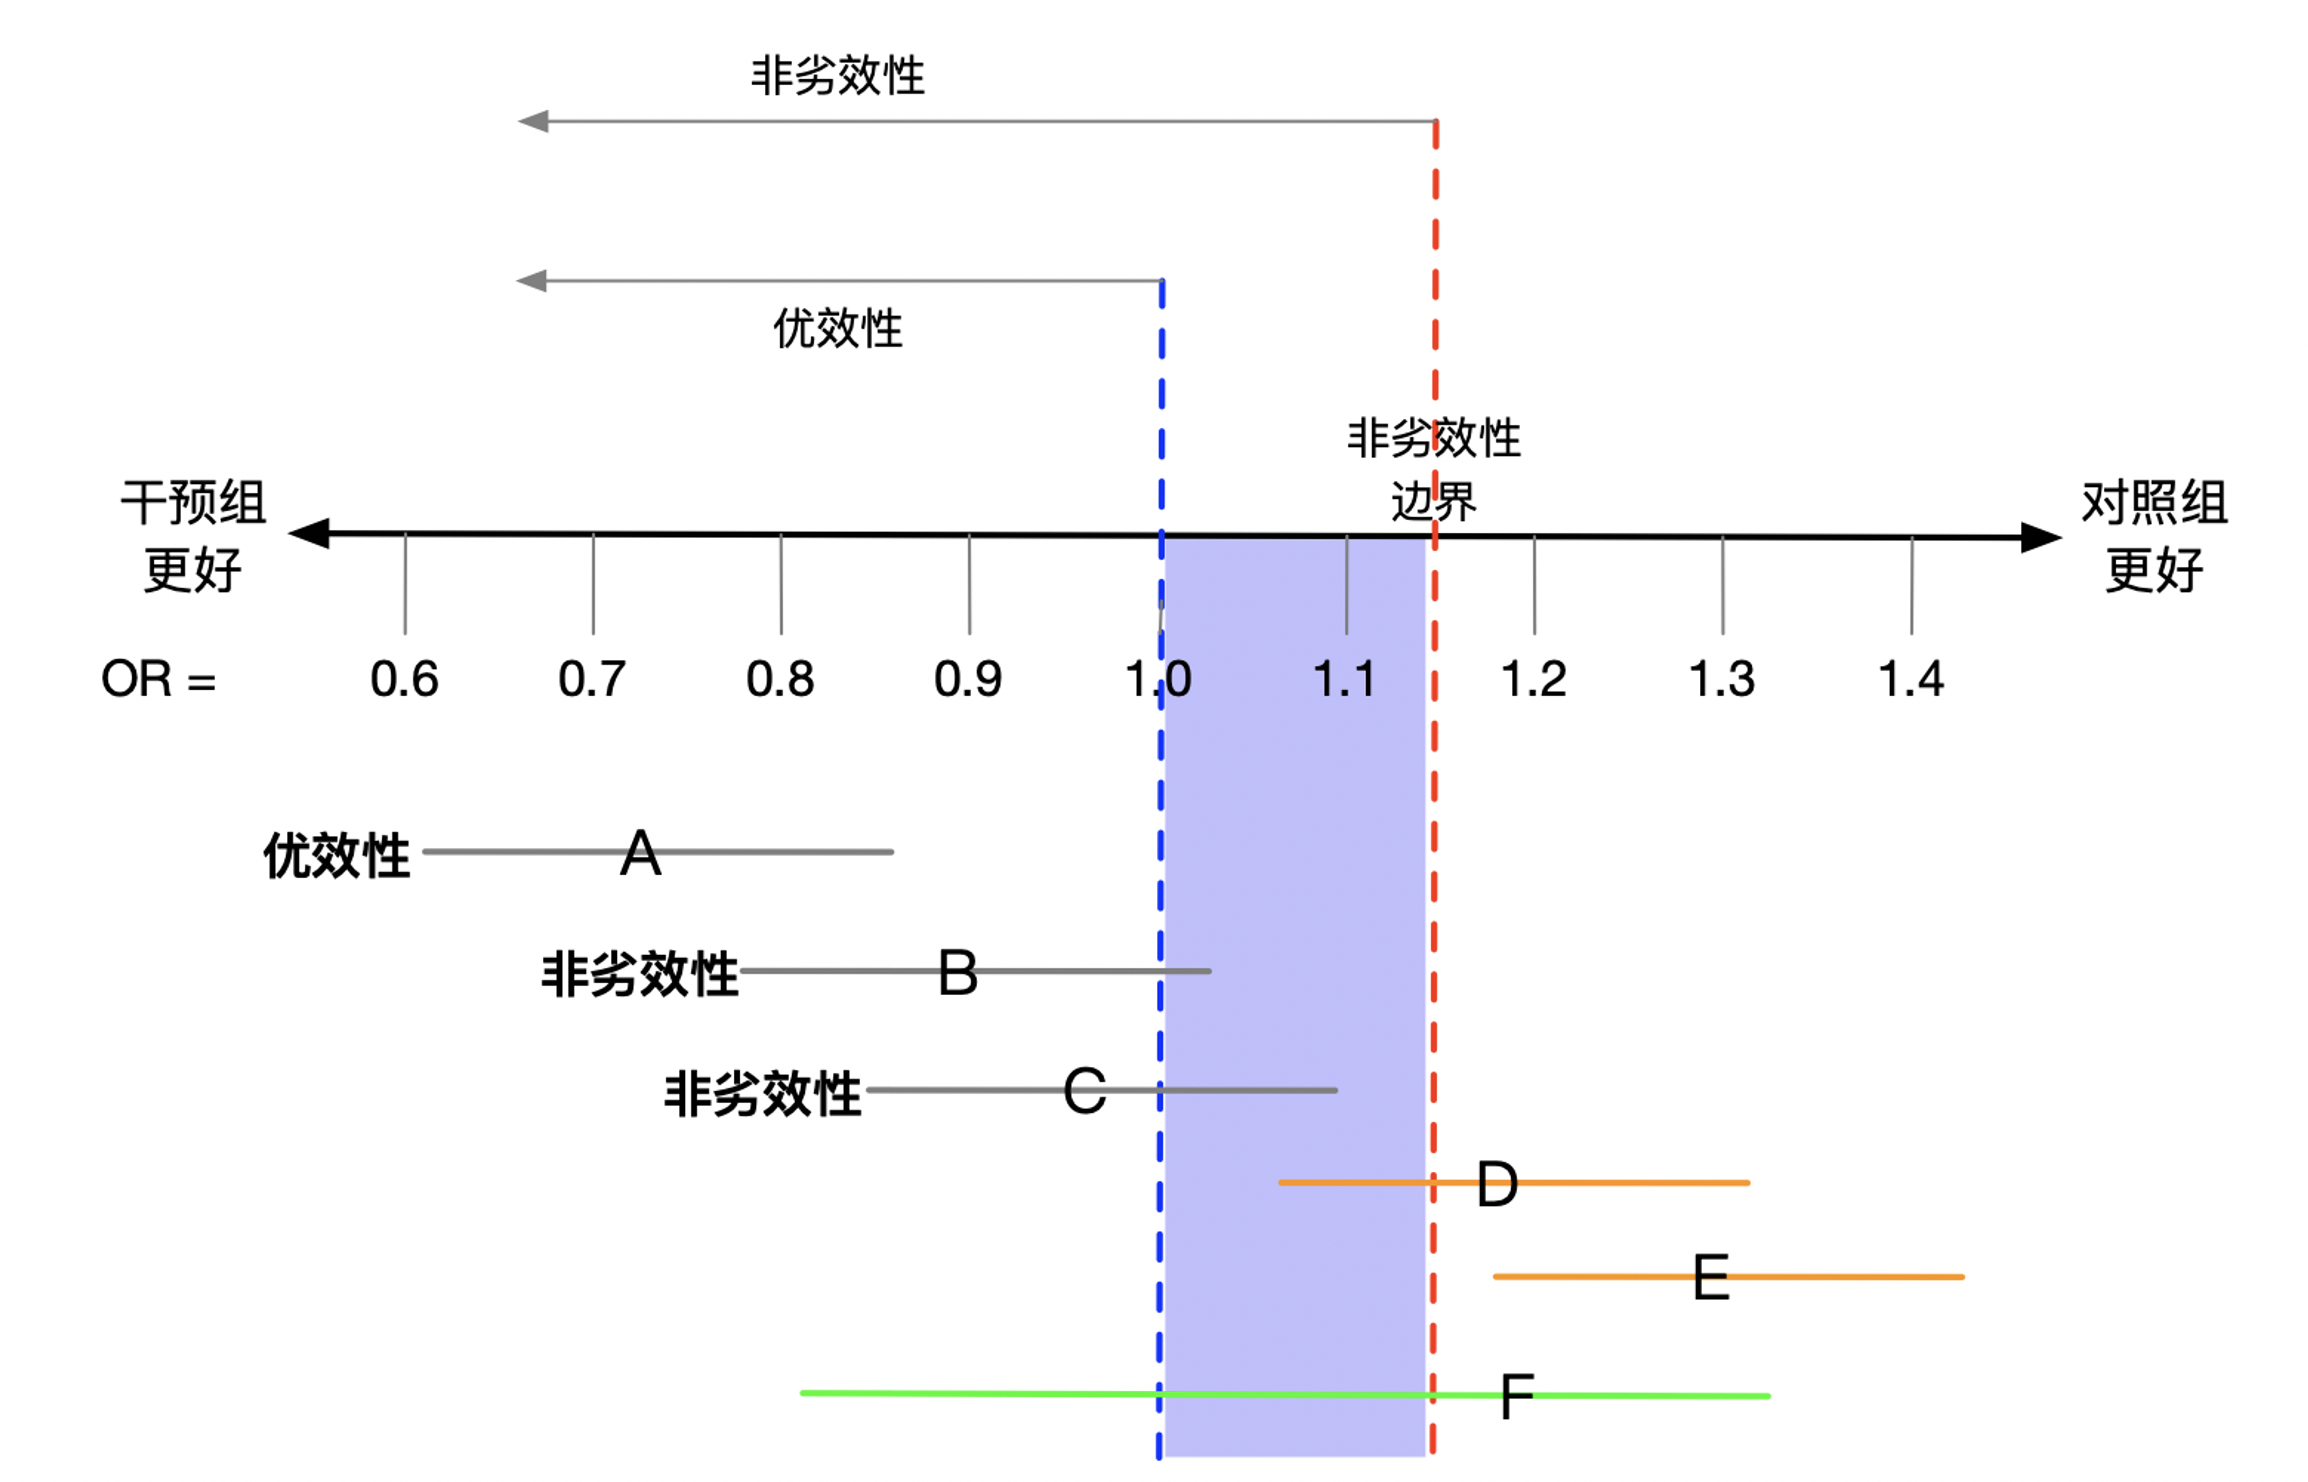
\includegraphics[keepaspectratio]{chapters/images/fig2-1.png}}

}

\caption{非劣效性边界图解}

\end{figure}%

图2.1中的横轴表示比值比，值为 1
处有一条蓝色虚线，这是优效性试验中的原假设。估计的比值比小于 1
表明新药更好，因为风险更小。1
的稍右侧有一条红色虚线，标记为非劣效边界。该值表示新药比华法林稍差，但差距在临床上没有意义，仍被视为非劣效的情况。A、B、C、D、E、F为假想的六个试验的点估计（字母位置）和95\%置信区间（线段长度）。

试验 A 比值比的点估计和 95\% 置信区间完全小于
1，这表明新治疗方法优于对照组。

试验 B 比值比的点估计小于 1，但 95\% 置信区间包含
1。因此，我们不能说新药比华法林更好。但由于整个 95\%
的置信区间都低于非劣效边界，我们可以说新药与华法林相比是非劣效的。

试验 C 与试验
B相同，亦满足非劣效性，因为置信区间的上限低于非劣效性边界。

试验 D
表明试验药物未达到非劣效性，因为置信区间的上限高于非劣效性边界。此外，由于整个
95\% 的置信区间显示华法林更好，实际上显示了华法林的优效性。

试验 E 表明新药比华法林差很多。

试验 F 有非常宽的置信区间，无法得出优越性或非劣效性的结论。

\section{实用性随机对照试验（Pragmatic Clinical
Trial）}\label{ux5b9eux7528ux6027ux968fux673aux5bf9ux7167ux8bd5ux9a8cpragmatic-clinical-trial}

常规的临床试验往往是经过最优化配置的，由经验丰富的研究人员参与，高度选择参与者，可能高估干预的益处而低估了其危害。这些研究成果亦难以转化为临床实践。实用性随机对照研究，常用于研究一项医疗卫生政策或者一项医疗决策能否改善受试者的预后。实用性研究尽量模拟常规医疗环境，其目标和真实世界相近，因此，开展实用性随机对照试验成为当前临床研究的热门，其主要特点有：实用性（pragmatic）与解释性（explanatory）试验的区分最早由
Schwartz 与
Lellouch（1967）提出：前者关注干预在常规医疗环境中的实际效果（effectiveness），后者关注理想条件下的生物学效力（efficacy）。研究者可借助
PRECIS-2
工具，在纳排标准、随访、依从性等多个维度上评估试验设计的实用性程度（Loudon
等，2015）。

\subsection{复杂度低}\label{ux590dux6742ux5ea6ux4f4e}

实用性随机对照试验尽量减少纳入和排除标准、减少研究的随访次数和复杂性从而增加试验的参与度。

\subsection{特殊情况下可豁免知情同意}\label{ux7279ux6b8aux60c5ux51b5ux4e0bux53efux8c41ux514dux77e5ux60c5ux540cux610f}

在某些情况下，获得伦理批准的前提下，可以在未经知情同意的情况下进行试验。例如，在
CRASH 试验中，超过 10,000
名头部外伤和意识受损的患者接受了随机分组，以确定与安慰剂相比，糖皮质激素是否会影响死亡率和神经功能障碍。在此研究中，由于激素的使用是在受伤后的很短时间内，且其风险被认为是最小，不干扰正常的临床治疗也不增加随访次数，该研究申请伦理委员会豁免知情同意。在涉及无法知情同意的背景下，赫尔辛基宣言指出，如果无法获得知情同意并且研究不能延迟，则可以在没有知情同意的情况下进行。

\subsection{通常不采用盲法}\label{ux901aux5e38ux4e0dux91c7ux7528ux76f2ux6cd5}

采用盲法的试验并不完全实用，可以想象在临床实践中给予患者的治疗都是确切的。在实用性设计中，随机分组通常不被遮蔽。因此，为尽量减少试验中产生的偏差，其主要终点事件往往都设定为可以客观评价的重大事件，例如死亡、急诊入院等等。

\subsection{无需额外的随访}\label{ux65e0ux9700ux989dux5916ux7684ux968fux8bbf}

实用性研究中，随访通常不增加受试者和研究人员的负担，且无需额外的随访。这种策略在具有可靠且可访问的电子健康记录的医疗保健系统中是最可行的，这些记录可以捕获感兴趣的事件。

\subsection{依从性评价}\label{ux4f9dux4eceux6027ux8bc4ux4ef7}

实用性研究并不强调所有受试者按照随机分配的方案完成研究，而将受试者的依从性评价也做为一个结局进行分析，依从性差提示该治疗在真实世界的临床实践中不可行。

\begin{enumerate}
\def\labelenumi{\arabic{enumi}.}
\setcounter{enumi}{5}
\tightlist
\item
  终点事件的确定和分析。
\end{enumerate}

实用性研究的终点通常很简单，可以最大限度地减少数据收集的要求。 CRASH
试验通过两页的病例报告表实现了高度简化，另一项导尿管试验的主要终点事件是出院后
6
周内出现的有症状的导尿管相关尿路感染，而不是实验室确认的院内感染。实用性试验通常使用邮寄问卷或基于网络的表格来避免来院随访，这种方法大大降低了研究成本。

\section{适应性随机对照试验（Adaptive Clinical
Trial）}\label{ux9002ux5e94ux6027ux968fux673aux5bf9ux7167ux8bd5ux9a8cadaptive-clinical-trial}

适应性随机对照研究是指在临床试验中，根据预先设计的规则，利用试验内部及外部积累的信息，动态地修改试验设计中的某些方面，而不破坏试验的有效性、科学性和完整性的一种设计。修改的内容包括干预的分配比例、总样本量和入组标准，试验可以从II期延长到III期，可以增加或取消治疗组。适应性设计有可能缩短试验完成时间，减少资源需求和无效治疗的病人数量，并从整体上提高试验成功的可能性。

常见的适应性临床试验类型包括：样本量重新评估、反应性适应性随机化、放弃无效治疗组、适应性富集、和无缝II-III期设计。基于试验期间实际的终点事件发生率来确定实际统计功效以重新评估样本量大小。反应性适应性随机化允许在试验期间改变随机化比例，因此，如果中期结果对干预组有利，新入组的受试者更有可能被分配到干预组。适应性富集是指对试验入组标准或结果评估的修改；如果中期分析显示某个亚组的反应更有利，可以通过修改入组标准来富集试验，使其只招募或主要招募该亚组的受试者。无缝适应性试验设计允许从一个阶段延续到下一个阶段，一般是从II期延续至III期试验。II期试验的结果可用于确定初始分配比例、计划的总样本量，随后的III期试验扩展至更大的人群。

适应性设计随机对照试验依旧拥有随机对照试验的随机化原则，也需要提前进行样本含量的估算，但不同的是在研究进行中可以根据预先设定的规则来确定下一阶段的样本量。在适应性设计中，常规的频率学派统计方法可能无法对个体治疗方案的调整进行预测，因此需引入贝叶斯统计利用先验信息对个体治疗方案进行预测。适应性设计在很大程度上依赖于计算机模拟，直到研究者和试验统计学家确信适应性设计的可能收益（预期减少所需的样本量、完成时间、避免的无效治疗次数）大大超过了潜在的风险（中期效果估计的风险、试验终止时计划统计分析的稳健性）。实施适应性试验通常涉及一个中期分析和决策的周期。决策规则是在试验开始前预先指定的，包括终止干预组或试验的数学表达、干预间分配比例的修改、预先指定的规则以重新估计样本量或缩小受试者入组标准、以及挑选新的干预组等等。

对于适应性设计，统计分析计划包括模拟、中期分析，以及对已完成试验的最终分析。适应性试验需要一个所谓的预处理阶段，在这个阶段可以按照固定的分配比例（通常是1:1）招募预定数量的病人，以确保收集到足够的数据，从而达到合理的预期精度。过早进行适应性调整可能会因为数据量小而更容易出现随机错误。反应性适应性随机化的一般经验法则是在每组至少收集20-30名受试者的数据后进行第一次中期分析。其他适应性，包括样本量的重新评估和富集，通常需要更长的预处理期和更大的样本量。在多臂适应性试验中，对照组的分配通常是固定的（如，占总样本量的20\%），而实验性治疗之间的分配比例是调整的。需要强调的是，适应性设计必须在研究方案中预先设定全部调整规则，并通过计算机模拟控制总体I类错误率，以免因多次中期分析而抬高假阳性风险；其方法学与报告规范可参考
Bhatt 与 Mehta（2016）以及 Pallmann 等（2018）。

I-SPY 2
是一项针对乳腺癌的适应性随机对照研究，其目标是根据患者的肿瘤分子生物标志物确定治疗方案。I-SPY
2
的总体试验设计，所有患者采用标准新辅助化疗方案，并同时测试五种新药，每一种新药都被添加到标准疗法中。患者在进行初步的活检、影像和血液检查后被随机分配到各个药物组，并在一定时间后评估治疗的反应。为了尽早获得有关治疗效果的信息，研究者对治疗反应与生物标志物之间的关系进行建模，并在试验期间不断评估结果，并将其作为依据确定随机化概率。试验过程中，研究者采用自适应随机化的贝叶斯方法，若研究过程中发现某种药物对携带特定生物标志物的受试者表现良好，则后续将此药优先分配给携带此特定生物标志物的其他受试者。当某种药物的疗效概率在所有患者中都下降到足够低时，该药物从试验中退出。研究结束时，比标准疗法更有效的药物与其相应的生物标志物特征，将在进一步的
III
期试验中进行测试。自适应设计方法可快速评估新药，识别有效的药物和药物组合，并确定哪些乳腺癌亚型将受益。随着试验的进行，研究可识别并使用来自每个患者的信息，并可为随后的治疗分配提供信息。

神经外科领域中的 GBM-AGILE 是一个类似于 I-SPY 2 的无缝 II/III
期胶质瘤临床研究平台，分两个阶段执行。该研究的第一阶段，多个研究组与共同的对照组进行比较，基于不同的生物标志物采用适应性随机化设计，评估研究药物对胶质瘤生存状态的影响。第一阶段中有显著效果的研究药物进入第二阶段，使用固定随机化设计来确认其治疗的有效性。这种研究设计方式能加速向受试者提供治疗机会，加快药物注册和监管审查。

\subsection{篮式研究（Basket
Trial）}\label{ux7beeux5f0fux7814ux7a76basket-trial}

具体的说，某种靶点明确的药物就是一个篮子，将带有相同靶基因的不同癌症放进一个篮子里进行研究就是篮式研究，其本质是一种药物应对不同的肿瘤。克唑替尼
A8081013
临床试验（NCT01121588）就是一项包括各种恶性肿瘤的篮式研究。此外，针对
BRAF 的篮式研究正在国内外如火如荼地开展着，BRAF
突变在多发性骨髓瘤、黑色素瘤、卵巢癌、结肠癌、甲状腺癌、绒毛膜癌、胃肠肿瘤、肺癌以及颅咽管瘤等多个癌种中被检出。

\subsection{伞式研究（Umbrella
Trial）}\label{ux4f1eux5f0fux7814ux7a76umbrella-trial}

同一种疾病，可能由不同基因驱动，如肺癌可由KRAS、EGFR、ALK
等驱动。这些同一疾病的不同亚型拢聚在同一把雨伞之下，根据不同的靶基因分配不同的精准靶药物。上一节提到的I-SPY
2和GBM-AGILE研究就属于伞式研究。

\section{随机对照研究结果阴性的解读}\label{ux968fux673aux5bf9ux7167ux7814ux7a76ux7ed3ux679cux9634ux6027ux7684ux89e3ux8bfb}

设计精良的随机对照研究有助于提升临床实践中的证据级别。虽然简单地根据 p
值是否小于 0.05
把一项研究归类为阳性结果和阴性结果非常不合理，但却是很普遍的做法。实际上
p 值应理解为连续的数字，p
值越小代表治疗效果的证据强度越大。此外，根据置信区间可以估计治疗效果的不确定性范围。对任何一项研究的解释还应参考证据的整体性（即主要、次要和安全性结果），而不仅仅是主要终点结局。

既往研究提示药物制造企业发起的新药临床研究中，只有 13.8\%（Wong
等，2019）
的研究最终获得批准得以上市。对于患者以及药物制造企业来说失败的随机对照研究（阴性结果）确实让人失望。对于神经外科疾病的临床研究来说，部分研究失败的原因中固然包括研究药物的生物学特性或神经外科疾病的特点，如药代动力学问题，疾病缺乏可靠的动物模型，中枢神经系统存在血脑屏障等。但部分研究出现阴性结果却还要归因于缺乏良好的研究设计。少部分研究者发起的临床研究因为资源受限而存在研究设计的瑕疵导致研究结论出现阴性结果，因而如何避免这些缺陷是未来继续开展随机对照临床研究需要进一步解决的问题。

根据研究假说，随机对照研究可分为优效性，非劣性以及等效性研究；根据随机方法来看，随机对照研究又可分为一般随机对照，群组随机对照以及交叉随机对照。在一项评估垂体肿瘤术前不使用糖皮质激素的安全性的研究中，由于该研究的主要假设是不使用糖皮质激素并不比使用糖皮质激素带来额外的并发症，因此，使用非劣性设计更适合此研究，但该研究中并没有采取这种方案。非劣性设计的另一大优势在于能明显减少样本量，增加研究效力。假设使用糖皮质激素组术后发生肾上腺功能不全的风险是5\%，不使用糖皮质激素组为10\%，通过统计计算可以得出：如果采取优效性研究设计总共需要864名患者，而采取非劣性设计只需要118名患者。此外，这项研究的另一个瑕疵在于其采取的随机方法。设想在同一个病房中同一天有两名受试者需要入组研究，如果没有很好的流程及人力保证的话，则很可能出现给不使用糖皮质激素组的受试者使用了糖皮质激素而导致受试者``被''换组。因此，采取群组随机方案会有效地避免这种情况，这个``群''往往是某个医疗机构，某个病房或某个时间段中就诊的病人群体，也就是在制定随机分组方案的时候，以医疗机构，病房或时间段为单位进行随机。群组随机可以提高受试者的依从性，因为经过群组随机以后受试者周边的其它``病友''基本上接受的是同样的治疗方案，研究者对受试者干预的管理非常统一，因此，不同组之间出现``污染''的情况会大大减少。

随机对照研究也需要考虑被研究的人群，因为不同人群可能对治疗的敏感性不同。一项评估氨甲环酸在脑外伤患者中有效性（CRASH-3）的研究中纳入了所有类型的脑外伤患者，终点事件是死亡。研究结果发现氨甲环酸组死亡率是18.5\%，安慰剂组死亡率是19.8\%，两者的比值比是0.94（95\%置信区间0.86-1.02，p大于0.05)。此研究可以被划分为阴性结果。然而，在分层分析中可以明显看出氨甲环酸在不同脑外伤人群中的治疗效果是不同的，在轻中度脑外伤患者中，氨甲环酸对比安慰剂的风险比值比是0.78（95\%置信区间0.64-0.95），但在重度患者中的风险比值比是0.99（95\%置信区间0.91-1.07），因此该研究得出结论氨甲环酸可能可以降低轻中度脑外伤患者的死亡率。一项在自发性脑出血患者中评估外科治疗对比保守治疗（STICH-I）的研究中，两组主要终点结局没有差别，但在亚组分析时该研究发现皮层出现亚组中早期手术能改善预后。因此，STICH-II针对浅表皮层血肿患者研究手术治疗对比保守治疗的效果，但遗憾的是该研究也没有确认手术治疗的优效性。此研究的亚组分析中也发现了人群存在异质性，预后好的患者可能手术治疗效果比保守治疗更好。另外一项替莫唑胺对比放疗治疗高风险低级别胶质瘤的随机对照研究（EORTC
22033-26033）中虽然在总人群中并没有获得阳性结果，但是亚组分析显示IDHmt/non-codel亚组中接受放疗组的无进展生存期更长。对于亚组分析的更深入讨论请参考第3章。

次要终点事件有时也可以为临床医师提供一些决策支持。上文中介绍的MISTIE-III研究次要终点事件为死亡率，统计分析提示微创治疗组死亡率明显比保守治疗组低，因此得出结论微创治疗可能降低自发性脑出血患者的死亡率。但需要注意的是无论是亚组分析还是次要终点在最终解释并指导临床决策时都需慎重，因为这些分析都涉及多重比较，犯I类错误的概率会大大提高，从而导致假阳性结果的出现。

随机对照研究受限于I类错误，往往只能纳入一个主要终点结局。神经外科领域中，有一些疾病有明确的终点事件，因此选择主要终点事件比较容易，如胶质瘤患者的生存状态，功能性垂体瘤的内分泌控制状态等。但对于脑外伤，脑出血性疾病来说，有不同的量表评估患者的功能状况，包括改良RANKIN量表（mRS），格拉斯哥预后量表（GOS）等等，选取终点事件时往往需要考虑不同的切点。一项在外伤性颅高压患者中比较去骨瓣减压手术与保守治疗的研究选取GOS作为主要终点事件。探索性结局的统计检验中，定义上肢重度瘫痪或更好作为切点将GOS评分作二分类处理，统计分析提示两组患者没有达到统计学差异，因而严格意义上来讲此研究也是阴性的。但如果从GOS结局的数据分布来看，去骨瓣减压手术能显著降低外伤性颅高压患者的死亡率（去骨瓣减压组26.9\%，对比保守治疗组48.9\%，p小于0.05）。此外，如果结局事件为多次测量的重复性事件（如功能性垂体瘤临床研究中的内分泌缓解）,传统的研究设计往往指定主要终点事件是治疗后第一次发生该事件，忽略随后发生的任何重复事件。近年来的一些研究表明，纳入多次测量结局作为终点事件有助于提高统计效力。

随机对照研究中还需要充分考虑受试者的依从性，治疗施与者的依从性，以及研究过程中有无违背研究方案的情况发生。一项国际多中心评估微创神经外科手术对比保守治疗干预脑出血（MISTIE-III）的研究，招募了506名自发性脑内出血的成年人，终点事件是治疗后365天受试者的神经功能状态（mRS量表0-3分为优良结局，4-6分为较差结局）。研究结果没有提供证据表明微创手术组对比保守治疗组能提高受试者的神经功能状态。但需要注意的是此研究中只有59\%的受试者在微创手术后达到了目标的血肿清除量（减小至少15mL），而既往研究表明血肿的清除量与结局之间是正相关的。此外，需要注意的是在药物/安慰剂对照研究中，由于盲法的存在，治疗交换很少发生，但在涉及手术/非手术对照的研究中，治疗交换是个大问题。另一项在自发性脑出血患者中评估外科治疗对比保守治疗（STICH-II）的研究中，虽然有294例受试者随机分配至保守治疗组，但其中有62例受试者在随机分配后改为手术治疗，治疗交换比例高达21\%。

由于阴性结果的判断是从统计学上出发的，因此统计学上阴性不等于临床上没有意义，有时还需要从临床上判断有无潜在的益处。一项评估氢化可的松或氟氢可的松对比安慰剂预防脑外伤后肺炎的研究（Corti-TC）中，统计学上未能显示激素使用后能降低医院获得性肺炎的风险，其风险比为0.75（95\%置信区间0.55-1.03，p大于0.05）。虽然在统计学上没有差异，但根据风险比为0.75可以看出潜在的风险减低达25\%，是否在临床上有意义值得商榷。另一项洛莫司汀联合替莫唑胺对比替莫唑胺单药治疗MGMT阳性胶质瘤的随机对照研究（CeTeG/NOA-09）中，主要终点指标为中位生存期，风险比为0.60（95\%置信区间0.35-1.03，p大于0.05），统计学上归为阴性结果。但是洛莫司汀联合替莫唑胺治疗组的中位生存期为48.1个月，而替莫唑胺单药组仅为31.4个月，平均增加的17个月临床上是有意义的。

临床研究得出阴性结果后还需要反思样本量是否充足。上文中的Corti-TC研究安慰剂组发生医院获得性肺炎远低于研究前的预期，因此导致实际上需要更多的样本才能检验出两组的差别。另一项研究评估了脑出血患者中微创神经外科手术对比保守治疗的预后（MISTIE）。微创治疗组30天的死亡率是9.5\%，而保守治疗组的死亡率是14.8\%，虽然两者统计学上没有显著差别，但两组总样本只有96例，远低于预期的样本量。

最后，意向性分析是几乎所有的随机对照研究中主要的分析方法。无论试验后续情况如何，当初所有参与随机分组的受试者均统统纳入分析。但有时意向性分析的阴性结果，可能是由于部分受试者违背研究方案引起的。近年来，符合方案分析作为后续探索性分析也经常在一些高质量的随机对照中研究中出现。如上述CeTeG/NOA-09研究中，有些中心出现了选择偏倚，探索性分析中剔除了这些中心后使用逆概率加权来矫正混杂因素后提示洛莫司汀替莫唑胺可能效果更好。但需要注意的是存在未测量混杂因素的情况下，符合方案分析仍然会引起偏倚。

\section{参考文献}\label{ux53c2ux8003ux6587ux732e-1}

\begin{enumerate}
\def\labelenumi{\arabic{enumi}.}
\item
  Thorlund K, Haggstrom J, Park JJ, Mills EJ. Key design considerations
  for adaptive clinical trials: a primer for clinicians. BMJ. 2018 Mar
  8;360:k698.
\item
  Lawrence F,~Curt F,~David D,~David R,~Christopher G. Fundamentals of
  Clinical Trials. Springer. 2015.
\item
  Schulz KF, Grimes DA. Generation of allocation sequences in randomised
  trials: chance, not choice. Lancet, 2002, 359(9305):515-519.
\item
  Schulz KF, Grimes DA. Allocation concealment in randomised trials:
  defending against deciphering. Lancet, 2002, 359(9306):614-618.
\item
  Schulz KF, Grimes DA. Blinding in randomised trials: hiding who got
  what. Lancet, 2002, 359(9307):696-700.
\item
  Schulz KF, Altman DG, Moher D, et al.~CONSORT 2010 statement: updated
  guidelines for reporting parallel group randomised trials. BMJ, 2010,
  340:c332.
\item
  Piaggio G, Elbourne DR, Pocock SJ, et al.~Reporting of noninferiority
  and equivalence randomized trials: extension of the CONSORT 2010
  statement. JAMA, 2012, 308(24):2594-2604.
\item
  Schwartz D, Lellouch J. Explanatory and pragmatic attitudes in
  therapeutical trials. Journal of Chronic Diseases, 1967,
  20(8):637-648.
\item
  Loudon K, Treweek S, Sullivan F, et al.~The PRECIS-2 tool: designing
  trials that are fit for purpose. BMJ, 2015, 350:h2147.
\item
  Bhatt DL, Mehta C. Adaptive designs for clinical trials. New England
  Journal of Medicine, 2016, 375(1):65-74.
\item
  Pallmann P, Bedding AW, Choodari-Oskooei B, et al.~Adaptive designs in
  clinical trials: why use them, and how to run and report them. BMC
  Medicine, 2018, 16(1):29.
\item
  Wong CH, Siah KW, Lo AW. Estimation of clinical trial success rates
  and related parameters. Biostatistics, 2019, 20(2):273-286.
\end{enumerate}

\bookmarksetup{startatroot}

\chapter{随机对照研究中的统计学考虑}\label{ux968fux673aux5bf9ux7167ux7814ux7a76ux4e2dux7684ux7edfux8ba1ux5b66ux8003ux8651}

\section{意向性分析与符合方案分析}\label{ux610fux5411ux6027ux5206ux6790ux4e0eux7b26ux5408ux65b9ux6848ux5206ux6790}

随机对照研究通常采用的分析策略是意向性分析（Intention to treat analysis,
ITT），即不论试验后续情况如何，当初所有参与随机分组的受试者均统统按照随机时的分组进行分析。与ITT分析相对应的是符合方案分析（Per-protocol
analysis,
PP），是对入组受试者按照实际遵循方案的情况进行分析。然而，对于ITT，往往存在三种认识误区。

首先，ITT得出的结果更倾向于无效吗？有一种误区认为如果干预的实际效应为无效，那么ITT应该比PP倾向于无效，这种认识是错误的。比如干预A和干预B的实际效应相同，理论上干预A和干预B的效应差应该为零。但在临床研究中由于干预A的副作用比较大，依从性比较差，导致疗效差。而干预B的副作用较小，依从性比较好，导致疗效好，按照这种情况得出的ITT结论会是干预B优于干预A。

第二种误区认为ITT更保守，这种认识也是错误的。假设干预A副作用较干预B大，干预A的受试者由于副作用比较大，依从性比较差，导致实际发生的副作用和干预B相似，那么ITT得出的结论会是干预A和干预B的副作用没有差别，但实际上干预A因为副作用比较大而更多地违背方案，这种结果不能称之为ITT更加保守。

第三种认识误区，认为ITT更反映真实世界，因为ITT的分析，考虑到了部分受试者依从性差的情况，而真实世界中总有部分患者依从性比较差。假设你是一位医生，一对夫妇想要了解某种避孕方法的有效性，那么，你会回答他们40\%的受试者没有正确使用该方法情况下的ITT分析显示这个方法的有效性是多少；还是回答，如果正确使用该方法情况下的PP分析显示该方法的有效性是多少？我想大部分的医生回答的应该都是后者。

在随机对照研究当中，由于神奇的随机化，ITT分析可以直接比较两个治疗组之间的差别。然而，PP分析中不仅在随机化前存在两组各项指标的不一致，随机化后也会因为受试者接受的治疗在两组中产生很多不一致的情况（如，根据患者的情况进行的药物剂量调整，由于副作用产生的失访等）。在随机对照研究中进行PP分析，其方法与非随机对照研究一样，也需要纠正这些随机前和随机后的混杂因素。而在随机对照研究设计与方案撰写的时候，也需要预先明确随机化后搜集哪些与预后相关的指标，以及明确如何进行PP分析。

用第1章的因果语言来说，ITT
分析估计的是``被分配（指派）到某干预''的因果效应（指派效应），它回答的是政策层面的问题，且因随机化而可直接识别；符合方案分析估计的则是``实际按方案接受干预''的效应，由于依从与否往往受随机化后的预后因素影响，朴素的
PP
分析会引入选择偏倚，需要像观察性研究那样校正随机化后的混杂（如逆概率加权），相关方法将在后续章节展开（Hernán
与 Hernández-Díaz，2012）。

\section{违背方案}\label{ux8fddux80ccux65b9ux6848}

违背方案的两种常见情况包括：

\subsection{不符合入组条件}\label{ux4e0dux7b26ux5408ux5165ux7ec4ux6761ux4ef6}

入组时违反方案规定，可能由于文书错误、实验室错误、错分类等原因。例如，在心肌梗死的多中心研究中，受试者因可能的急性心肌梗死入院，予干预组或安慰剂治疗。然而，心肌梗死的诊断是在监测了数天的心电图和血清酶变化后才确认的。部分受试者在初步诊断为心肌梗死的基础上参与了随机分配，后续的心肌酶谱监测却不支持最初的诊断。

更复杂的情况是，给予受试者的干预可能会影响或改变入组条件。例如，在上述心肌梗死的研究中，如果干预措施成功地限制了梗死面积，可能会影响心电图和血清酶水平，从而影响心肌梗死的诊断。而安慰剂组则不可能存在这种情况。对照组中不符合入组条件的参与者很容易被识别出来，而干预组中真正不符合入组条件的受试者必须与那些因干预效果而显得不符合的受试者区分开来。

鉴于此，随机对照研究设计时可遵从三种策略。策略一、诊断得到确认并仔细检查之前，不得入组。策略二、确需删除不符合入组标准的受试者，所依据的信息需基于入组前收集的数据，且决定人需保持结局与分组分配的盲法。策略三、允许不符合入组标准的受试者入组，但不允许退出，因为两组有同等的机会纳入不符合入组标准的受试者，但可能会因为不符合入组标准的受试者存在而减少结局事件的差异。

\subsection{依从性}\label{ux4f9dux4eceux6027}

不遵守方案是受试者退出分析的另一个原因。不依从的另一种形式是失访。不依从可能是由于干预组或对照组中的不良事件、兴趣或感知利益的丧失、潜在状况的变化或各种其他原因。不依从性对试验结果的影响是，与对照相比，干预的任何益处都将减少，从而使试验所需样本量大于计划。其次，如果某组中的不依从性比另一组更大，且不依从与结果相关，那么不依从受试者的退出可能会导致偏倚。最好的策略是设计试验时考虑将不依从性降至最小，然后使用ITT分析结果。

不依从性的定义也会对分析产生重大影响。临床研究实践中可以将依从性定义为受试者实际接受的干预与方案规定干预的匹配比例。在药物/安慰剂的临床试验中需要分别描述干预组与对照组的依从性，如果干预组的依从性低于对照组，则可能无法合理预期该疗法在临床实践中的广泛使用。即，干预可能是有效的，但如果大部分受试者不能忍受，则可能没有什么价值。

\section{多重比较}\label{ux591aux91cdux6bd4ux8f83}

假设张三在玩猜硬币游戏，连猜五次后发现他次次都猜中。于是我们认为他在作弊，因为如果他没作弊的话，连续猜对五次的概率只有

\textbf{公式3.1　连续猜中五次的概率}

\[{0.5}^{5}\  \approx \ 0.03\]

然而当100个人同时玩猜硬币游戏，每个人猜五次，然后发现只有李四连猜五次都猜对了。那么，是不是能像前面一样，认为李四在猜硬币时作弊了呢？简单计算一下就可以发现，当100个人猜硬币时，出现一人或以上五次都猜对的概率为

\textbf{公式3.2　100人中至少一人连续猜中五次的概率}

\[1 - {(1 - 1/32)}^{100} = \ 0.958\]

\begin{tcolorbox}[enhanced jigsaw, arc=.35mm, bottomrule=.15mm, breakable, colback=white, colframe=quarto-callout-note-color-frame, left=2mm, leftrule=.75mm, opacityback=0, rightrule=.15mm, toprule=.15mm]

\vspace{-3mm}\textbf{代码3.1}\vspace{3mm}

\begin{Shaded}
\begin{Highlighting}[]
\NormalTok{p\_one }\OtherTok{\textless{}{-}} \DecValTok{1} \SpecialCharTok{/} \DecValTok{2}\SpecialCharTok{\^{}}\DecValTok{5}                 \CommentTok{\# 一个人连对 5 次}
\NormalTok{p\_any }\OtherTok{\textless{}{-}} \DecValTok{1} \SpecialCharTok{{-}}\NormalTok{ (}\DecValTok{1} \SpecialCharTok{{-}}\NormalTok{ p\_one)}\SpecialCharTok{\^{}}\DecValTok{100}     \CommentTok{\# 100 人中至少一人连对 5 次}
\FunctionTok{c}\NormalTok{(单人 }\OtherTok{=}\NormalTok{ p\_one, }\StringTok{\textasciigrave{}}\AttributeTok{100人至少一人}\StringTok{\textasciigrave{}} \OtherTok{=}\NormalTok{ p\_any)}
\end{Highlighting}
\end{Shaded}

\end{tcolorbox}

\begin{tcolorbox}[enhanced jigsaw, arc=.35mm, bottomrule=.15mm, breakable, colback=white, colframe=quarto-callout-note-color-frame, left=2mm, leftrule=.75mm, opacityback=0, rightrule=.15mm, toprule=.15mm]

\vspace{-3mm}\textbf{代码3.1输出}\vspace{3mm}

{\def\LTcaptype{none} % do not increment counter
\begin{longtable}[]{@{}lr@{}}
\toprule\noalign{}
情形 & 概率 \\
\midrule\noalign{}
\endhead
\bottomrule\noalign{}
\endlastfoot
单人连续猜中五次 & 0.0312500 \\
100人中至少一人连续猜中五次 & 0.9582005 \\
\end{longtable}
}

\end{tcolorbox}

显然，这时我们就不能再说李四在作弊了。

统计学的假设检验基本原理是小概率原理，即认为小概率事件在一次试验中实际上不可能发生。但当同一研究进行多次假设检验时，不再符合小概率原理所说的``一次试验''。

1992年瑞典有研究者试图找出高压电线对健康的影响，他们收集了高压电线300米范围内所有住户的样本，在长达25年的时间内，对超过800种疾病一一检查其发生率与高压电线外住户的统计差异。他们发现幼年白血病的发病率是一般人的4倍，因此推动政府为此采取行动。此研究的问题就出在多重比较中，当比对超过800种疾病时，有一种以上的疾病因为随机效应而呈现发病率增加是非常可能的。在多重比较中需区分两类错误控制目标：一类是控制总体犯一类错误的概率（族系错误率，FWER），Bonferroni
法、Holm
法等属此类；另一类是控制错误发现率（FDR），即被拒绝的假设中假阳性所占的期望比例，Benjamini--Hochberg
法属此类，在大规模探索性检验中更不保守。随机对照试验中多重性问题的系统讨论可参考
Schulz 与 Grimes（2005）。

临床研究中需要考虑多重比较问题的情况有如下几种：

\subsection{存在多个主要疗效指标}\label{ux5b58ux5728ux591aux4e2aux4e3bux8981ux7597ux6548ux6307ux6807}

临床研究中的多重比较问题通常是选择了多个主要结局。解决方法为选择一个最重要的结局为主要结局，其他的作为次要结局，用主要结局的结果来决定试验的结果；或者将几个指标构建成一个复合结局作为主要结局进行分析。如果确需采用多个主要结局，需要考虑多重性问题。

1）当要求多个指标同时有统计学意义，才认为试验有效，此时无需校正α。

2）只要有一个指标有效，即认为试验药物有效，此时需校正α；一般按重要性进行分配，重要的指标检验水准大一些，不重要的指标检验水准小一些，也可以等分，但总和不超过α。可采用简单的Bonferroni法矫正，

\textbf{公式3.3　Bonferroni校正}

\[\text{矫正}\alpha\text{值} = 0.05/n\]

n为主要结局的数量。Bonferroni法非常简单，但缺点在于非常保守，尤其当n很大时，经过Bonferroni法矫正后总的一类错误可能会远远小于既定α。

3）按指标的重要性排序，进行序贯检验，即从最重要的指标开始，依次进行假设检验，当前一个假设检验拒绝原假设时，方可进行下一个指标的假设检验；如果前一个假设检验不拒绝原假设，则停止所有后续指标的检验，并由此推断后面的指标组间差异均无统计学意义。这种情况不需要校正α。由于假设检验的顺序将直接影响统计结果，因此，指标的检验顺序的确定需在方案中事先明确声明。揭盲后再确定或调整检验顺序的做法是绝对禁止的。

\subsection{多组间疗效指标比较}\label{ux591aux7ec4ux95f4ux7597ux6548ux6307ux6807ux6bd4ux8f83}

1）如果组间是剂量大小关系，则可以采用序贯检验。即按剂量组由高到低的顺序逐一与对照组比较，对多个假设进行检验。此时也不需要校正α。

2）如果组间没有剂量大小关系，则需要校正α。例如试验组与安慰剂对照组、阳性对照组相互比较，常采用Bonferroni校正α至α/n，这里n是比较的次数。

\subsection{复合指标}\label{ux590dux5408ux6307ux6807}

1）复合指标是由不同的分指标加权合并而成（如，评分量表），或由不同的指标定义（如，主要不良心血管事件），当复合指标有统计学意义时，再对每个分指标进行假设检验，无需校正α；

2）无论复合指标是否有统计学意义，都对每个分指标进行假设检验，且只要有一个指标有统计学意义，即认为试验药物有效。此时需校正α。

\subsection{同一个主要疗效指标，比较的类型发生改变}\label{ux540cux4e00ux4e2aux4e3bux8981ux7597ux6548ux6307ux6807ux6bd4ux8f83ux7684ux7c7bux578bux53d1ux751fux6539ux53d8}

这种情况常见于先将试验组和阳性对照组比较，进行非劣效检验。如果非劣效性成立，再进行优效性检验，此时不需要校正α。

\section{期中分析与α消耗}\label{ux671fux4e2dux5206ux6790ux4e0eux3b1ux6d88ux8017}

期中分析是临床试验正式完成前，根据事先制订的统计分析计划，对干预组和对照组间的有效性和安全性所进行的分析。由于期中分析的次数、方法及结果将对试验结果的解释产生影响，所有期中分析必须预先在试验方案中阐明。特殊情况下，期中分析未能在试验开始前确定，至少应在最终的统计分析前完善期中分析方案并修改试验方案。

期中分析一般有三个目的：

\subsection{及时监测临床试验的安全性}\label{ux53caux65f6ux76d1ux6d4bux4e34ux5e8aux8bd5ux9a8cux7684ux5b89ux5168ux6027}

如果干预出现安全性问题，则提前终止试验。

\subsection{尽早确认干预的有效性}\label{ux5c3dux65e9ux786eux8ba4ux5e72ux9884ux7684ux6709ux6548ux6027}

如果试验有效并达到预先设定的标准，可以提前因有效而终止；如果试验无效低于预先设定的标准，可以提前因无效而终止；避免后续研究费事费力费钱。

\subsection{样本量的重新估计}\label{ux6837ux672cux91cfux7684ux91cdux65b0ux4f30ux8ba1}

由于试验设计时先验信息有限，对干预组的有效性或安全性估计不尽准确，导致样本量的估计也不够准确，期中分析时可以重新估计样本量，计算后验概率，确保试验有足够的把握度。

绝大多数的期中分析是为了证明干预措施的有效性，此时则需要考虑控制假阳性率（I类错误率）。因为，每进行一次期中分析，即进行一次假设检验，根据上述多重检验的原则，会使假阳性或I类错误率增加。如果每一次期中分析时研究者都采用α=0.05的检验水准，那么最后的总体α
水平随着检验次数而升高。为了使研究的总体I类错误控制在检验水准α
(0.05)，则必须校正每一次期中分析的检验水准。即，每一次期中分析都会消耗一定比例的α，期中分析越多，消耗的α越多，留给最终分析的α越少。

由于期中分析的结果会对后续试验的结果产生影响，因此，期中分析的日程、安排、α
消耗或分配等应当事先制订计划并在试验方案中阐明。各阶段检验水准、检验效能及样本量受到α消耗方法的影响，常用的α消耗方法有以下三种:
Pocock法、O'Brien-Fleming法和Peto法。

Pocock较简易，进行一次期中分析和一次最终分析，共分析两次，为控制总检验水准为0.05，两次α均为0.029。其缺点是最后一次α远小于0.05。若期中分析未得到阳性结果，则最终研究不易得到阳性结果。

O'Brien-Fleming法，简称O-F
法，该法在期中分析时采用严格的标准，而随着试验的进行，信息逐渐累积，使结果变得可靠与稳定，此时α也随之放宽，最后一次分析的α较接近0.05。如果研究继续进行达到计划的样本，那么最终的分析如同没有期中分析一样。因此，用O-F
法来设计试验与传统试验很相似，而且当试验组被证明有很强的优势时可以提早终止试验。

Peto法与O-F法类似，期中分析时采用严格的标准，而最后一次的α更接近0.05。其易于理解、执行与描述。但由于要求早期终止的α很小（0.001），一般认为用Peto法早期终止研究比较困难。上述方法可统一在
α 消耗函数（alpha spending function）框架下理解：DeMets 与
Lan（1994）指出，只要预先设定 α
随信息量累积的消耗方式，便可灵活安排期中分析的时点与次数，而无需事先固定；Pocock（1977）与
O'Brien-Fleming（1979）则分别对应消耗较快与早期严格、消耗较慢的两类经典边界。

\textbf{案例3.1}

KEYNOTE-604是一项随机、双盲、Ⅲ期临床研究，符合条件的453例肺癌患者，按照1:1随机分配接受帕博利珠单抗或安慰剂治疗35个周期或至疾病进展。主要终点为无进展生存和总体生存。预先设定两次期中分析和一次最终分析，第一次期中分析的α为0.0024，第二次期中分析的α为0.0071，最终分析的α为0.012。

两次期中分析都没有得到阳性的结果。最终分析显示，帕博利珠单抗和安慰剂组中位总体生存率分别为10.8个月和9.7个月，在意向治疗人群中未达到显著性（危险比0.80；95\%
置信区间0.64-0.98；p =
0.016）。虽然生存曲线最终呈现明显分开的趋势，0.016和0.012的微弱差距却造就了阴性结果。期中分析对α的消耗不容忽视，如果没有期中分析，OS就可以得到阳性的结果。之所以强调临床医生对于统计方法学的理解，是不希望一个临床上有显著差异的案例，由于统计设计/分析方法的失误而得到阴性结果，导致浪费大量的人力物力和时间。

\section{亚组分析}\label{ux4e9aux7ec4ux5206ux6790}

随机对照研究中常见的分析技术是根据基线特征对受试者进行分组，以评估不同亚组的患者对干预的反应是否不同。亚组分析可以支持或详细说明试验的总体效应，亦可对特定亚组提供探索性结果。然而，在解释亚组发现时必须小心谨慎，因为亚组分析的结果通常具有误导性。针对亚组分析的具体建议包括如下几点。

\begin{enumerate}
\def\labelenumi{\arabic{enumi}.}
\tightlist
\item
  亚组分析应该预先指定。
\end{enumerate}

由于在试验结束后通过对数据的持续探索几乎总是可以找到至少一个暗示性的亚组效应，建议在研究方案中预先指定需要分析的亚组以及每个亚组的生物学合理性。此外，用于分层随机化的因素（例如年龄、性别或疾病阶段）在研究设计中已被暗示为亚组，即使它们没有在方案中明确说明。没有生物学合理假设支持的亚组更应谨慎对待。部分亚组分析为事后分析，有时称为``数据挖掘''或``钓鱼''。此类分析应主要用于生成假说以在其他试验中进行验证。

\begin{enumerate}
\def\labelenumi{\arabic{enumi}.}
\setcounter{enumi}{1}
\tightlist
\item
  亚组分析应该进行多重比较的矫正。
\end{enumerate}

如果要对大量亚组进行显着性检验，假阳性结果的可能性会增加。因此，可以通过诸如Bonferroni校正或其他多种检验的矫正方法来完成。如果一项研究发现干预和对照之间的差异似乎集中在特定的亚组中，那么需要检索相同的结果是否出现在另一类似的试验中。

\begin{enumerate}
\def\labelenumi{\arabic{enumi}.}
\setcounter{enumi}{2}
\tightlist
\item
  应该使用交互作用而不是采用组内估计效果。
\end{enumerate}

既往文献的共识强烈支持交互作用的方法，提供了亚组分类变量是否与治疗效应相关联的全局评估，并给出这些效应的点估计及其置信区间。相比之下，亚组内治疗效果的估计需要更多的假设检验，并且会夸大假阳性结果的概率。

总之，亚组分析可能会出现较大的随机差异，其发现很容易被过度解释。观察到的不同亚组之间结果的差异并不意味着干预的效果是不均匀。若试验的主要效应没有显着性，研究者在报告重要的亚组发现时应特别保守。关于亚组分析的可信度，Wang
等（2007）在《新英格兰医学杂志》系统提出了上述原则（预先设定、交互作用检验、多重性校正等）；Sun
等（2010）进一步给出了评估亚组效应是否可信的系列标准，如该亚组假设是否事先提出、是否有交互作用检验支持、是否在独立研究中得到重复等，可作为解读亚组结果的实用清单。

\section{多中心临床研究}\label{ux591aux4e2dux5fc3ux4e34ux5e8aux7814ux7a76}

涉及多中心的临床试验中评估治疗方法非常常见，主要是因为一个中心很少能招募足够数量的患者来完成试验。因此，对多中心临床试验进行统计分析要考虑中心效应，以便更好地了解总体平均治疗效果、治疗效果的变异性以及不同中心的效应。在多中心试验中，随机分组通常按中心分层，以实现每个中心接受每种治疗的平衡。

可使用两种不同的统计模型分析多中心临床试验结果。首先，可使用一个简单的模型，不包括中心效应项，所有的变异性都被认为只来自于受试者，没有任何中心与中心之间的系统差异。第二，可使用一个更合适的模型，将单个中心内受试者的变异性与中心的变异性分开。第一个模型中没有中心效应，将高估平均治疗效果的变异性，因为它假定所有的变异性都是受试者群体的固有特征，这将导致置信区间过宽，统计效能下降。相反，包含中心效应的模型将正确认识到一些变异性是每个中心治疗人群的差异特征，这将减少单个中心内部受试者的变异性，从而增加估计精度。

在估计治疗效果时，可以使用各种统计模型来考虑中心效应。最简单的方法是将中心视为固定效应。这种方法可用于线性模型、生存分析或逻辑回归，在每种情况下，都允许在一个中心内的治疗结果与不同中心的治疗结果之间有更大的相似性。

\section{附录：新英格兰医学杂志的统计学规范}\label{ux9644ux5f55ux65b0ux82f1ux683cux5170ux533bux5b66ux6742ux5fd7ux7684ux7edfux8ba1ux5b66ux89c4ux8303}

\subsection{所有研究}\label{ux6240ux6709ux7814ux7a76}

\begin{itemize}
\item
  所有论文的方法部分应说明该研究对于样本量和统计学功效的考虑，并简要说明主要结局和次要结局的分析方法。
\item
  所有论文的方法部分应说明如何处理缺失数据。除非数据缺失很少，否则只分析具有完整信息的病例集一般不能作为主要分析，而应基于数据缺失机制，使用适当的方法插补。当数据随机缺失时，可采用多重填补法或逆概率加权法；当数据缺失非随机，基于模型的方法更适合。
\item
  显著性检验中统计效应值、相关性或其它参数的点估计值都应附有相应的置信区间。置信区间应根据α进行校正。
\item
  除非研究设计（如非劣效性临床试验）要求进行单侧检验，否则所有报告的 p
  值都应是双侧检验。一般而言，大于0.01的 p
  值应保留两位小数，0.01\textasciitilde0.001之间的 p
  值应保留三位小数；小于0.001的 p 值应报告为p \textless{}
  0.001。除此之外，预先设定终止规则的临床试验所获得的 p
  值，或全基因组关联研究所获得的 p
  值，其报告精度可不受上述位数规则的约束。
\item
  报告结果时，精确度不应超过科学意义和样本量所界定的精确度。例如，比值比一般应报告两位小数。
\end{itemize}

\subsection{临床试验}\label{ux4e34ux5e8aux8bd5ux9a8c}

\begin{itemize}
\item
  原始和最终试验方案及统计分析计划应在投稿时一并提交，并且需要提交对试验方案做出的修正列表，以说明修订日期和修订内容。
\item
  主要结局的分析应与原始试验方案中预先设定的分析一致。试验方案中未列出的分析应在论文的方法部分说明理由。编辑可能要求作者补充提交试验方案中未包含的分析。
\item
  比较两组或多组结局时，研究者应采用试验方案中设定的检验程序来控制总的一类误差。对于预先设定的探索性分析，研究者应采用研究方案中说明的一类错误的控制方法，例如Benjamini--Hochberg分析。（即
  Benjamini--Hochberg 法，用于控制错误发现率；Benjamini 与
  Hochberg，1995。）
\item
  如果临床试验的试验方案中未设定多重性校正方法或一类错误控制方法，则对所有次要和探索性终点的报告应仅限于疗效的点估计值和95\%置信区间。在这种情况下，方法部分应说明置信区间宽度未进行多重性校正，由此得出的推论可能无法重复。这些分析不应报告
  p 值。
\item
  在研究方案中预先设定了亚组分析的情况下，该分析应符合研究方案中描述的方法。如果研究团队认为对亚组进行事后分析具有重要意义，则应说明进行此项分析的理由，并在论文中清楚注明这属于事后分析。
\item
  森林图常用于呈现所关注的各亚组中的疗效一致性。该图可有效显示各亚组的估计疗效，建议在论文中给出重要亚组的森林图。治疗与亚组之间交互作用的一系列p值可能存在多重性问题，用于推断的价值有限。因此，在大多数情况下，森林图中不应提供交互作用的
  p 值。
\item
  如果安全性结局（不是主要结局时）的显著性检验与特定治疗的估计值一起报告，则无需进行多重性校正。因为安全性终点包含的信息大于0.05的一类错误是可接受。
\item
  研究中在报告风险差（Risk difference）或风险比（Risk
  ratio）之前应报告事件绝对数量或发生率，目的是向读者提供事件的实际发生率。应避免使用比值比（Odds
  ratio），因为在许多情况下可能高估相对危险度并且被错误解读。
\item
  研究者应提供CONSORT格式的流程图，提交CONSORT清单中包含的所有相关信息。
\end{itemize}

\subsection{观察性研究}\label{ux89c2ux5bdfux6027ux7814ux7a76}

\begin{itemize}
\item
  观察性研究结果的有效性取决于样本的选择、测定和未测定的混杂因素以及混杂因素的控制方法。观察性研究的方法部分应说明在研究设计和分析中如何处理这些问题。
\item
  如果一项观察性研究包含了预先设定的统计分析方案，则投稿时应附上签署了姓名和日期的统计分析方案。
\item
  如果观察性研究涉及多重检验，应采用预先设定的方法来控制一类错误。在未预先设定错误控制方法的观察性研究论文中，统计量应仅限于点估计值和95\%置信区间。在这种情况下，方法部分应说明置信区间宽度未进行多重性校正，所得推断可能无法重复，且这些分析不应报告
  p 值。
\item
  方法部分应列出计划的分析方法，包括选择病例时的纳入标准和数据采样方法，适当的情况下可附上图表。说明待估计的关联或因果关系，以及做出该选择的理由。
\item
  报告治疗效应的研究应说明潜在混杂因素和其他变量在不同治疗组间的分布。
\item
  复杂模型最好在补充附录中加以说明。对于未测定的混杂因素所造成的偏倚，研究中应通过敏感性分析来讨论不同设定对上述偏倚的影响；如未进行此项分析，则必须讨论未测定的混杂因素所造成的潜在偏倚。
\item
  研究者应在类似的但独立的一项或多项研究中重复研究结果，以评估稳健性。
\end{itemize}

\section{参考文献}\label{ux53c2ux8003ux6587ux732e-2}

\begin{enumerate}
\def\labelenumi{\arabic{enumi}.}
\item
  Lawrence F,~Curt F,~David D,~David R,~Christopher G. Fundamentals of
  Clinical Trials. Springer. 2015.
\item
  Senn SJ, Lewis RJ. Treatment Effects in Multicenter Randomized
  Clinical Trials. JAMA. 2019 Mar 26;321(12):1211-1212.
\item
  The New England Journal of Medicine.
\item
  Hernán MA, Hernández-Díaz S. Beyond the intention-to-treat in
  comparative effectiveness research. Clinical Trials, 2012, 9(1):48-55.
\item
  Montori VM, Guyatt GH. Intention-to-treat principle. CMAJ, 2001,
  165(10):1339-1341.
\item
  Schulz KF, Grimes DA. Multiplicity in randomised trials I: endpoints
  and treatments. Lancet, 2005, 365(9470):1591-1595.
\item
  Pocock SJ. Group sequential methods in the design and analysis of
  clinical trials. Biometrika, 1977, 64(2):191-199.
\item
  O'Brien PC, Fleming TR. A multiple testing procedure for clinical
  trials. Biometrics, 1979, 35(3):549-556.
\item
  Peto R, Pike MC, Armitage P, et al.~Design and analysis of randomized
  clinical trials requiring prolonged observation of each patient. I.
  Introduction and design. British Journal of Cancer, 1976,
  34(6):585-612.
\item
  DeMets DL, Lan KK. Interim analysis: the alpha spending function
  approach. Statistics in Medicine, 1994, 13(13-14):1341-1352.
\item
  Wang R, Lagakos SW, Ware JH, et al.~Statistics in medicine - reporting
  of subgroup analyses in clinical trials. New England Journal of
  Medicine, 2007, 357(21):2189-2194.
\item
  Sun X, Briel M, Walter SD, et al.~Is a subgroup effect believable?
  Updating criteria to evaluate the credibility of subgroup analyses.
  BMJ, 2010, 340:c117.
\item
  Benjamini Y, Hochberg Y. Controlling the false discovery rate: a
  practical and powerful approach to multiple testing. Journal of the
  Royal Statistical Society: Series B, 1995, 57(1):289-300.
\end{enumerate}

\bookmarksetup{startatroot}

\chapter{随机对照研究方案与受试者知情同意的撰写}\label{ux968fux673aux5bf9ux7167ux7814ux7a76ux65b9ux6848ux4e0eux53d7ux8bd5ux8005ux77e5ux60c5ux540cux610fux7684ux64b0ux5199}

随机对照研究开展前重要的步骤是方案以及受试者知情同意的撰写。本章介绍撰写的要点，并附以案例以供读者参考。规范的方案撰写可遵循
SPIRIT 2013 声明（标准方案条目：干预性试验的建议），它提供了一份涵盖 33
个条目的方案清单；此外，试验在纳入受试者前应在公开的临床试验注册平台（如
ClinicalTrials.gov 或中国临床试验注册中心）进行前瞻性注册（Chan
等，2013）。

\section{随机对照研究的方案撰写}\label{ux968fux673aux5bf9ux7167ux7814ux7a76ux7684ux65b9ux6848ux64b0ux5199}

\begin{enumerate}
\def\labelenumi{\arabic{enumi}.}
\tightlist
\item
  研究背景
\end{enumerate}

研究方案需提供相关的研究背景，以说明研究问题的重要性和必要性，以及预期获益，并列出与研究背景相关的文献和数据。应说明此项研究相关的前期研究结果，包括实验室研究、动物实验研究、以及科学文献和其它相关信息和数据，以支持研究的合理性，列出国内外研究进展和本研究的创新点。

在满足上述条件的基础上，一般的研究背景撰写思路是：研究问题的相关定义介绍；目前的现状，现状存在什么问题或缺陷；针对这些问题国内外研究进展；本研究计划做些什么，有哪些创新点和临床意义或社会价值；本研究内容有哪些前期工作基础或基本条件，目前计划开展本研究和研究设计的立题依据、科学性和可行性，遵循法规情况；本研究可能存在哪些风险，选择研究对象的考虑依据，对这些研究对象是否有获益，获益是否大于存在的风险。

\begin{enumerate}
\def\labelenumi{\arabic{enumi}.}
\setcounter{enumi}{1}
\tightlist
\item
  研究目的
\end{enumerate}

任何一项研究都必须有明确的研究目的，即这个研究将要回答或解决什么问题。以药物临床研究为例，研究目的基本围绕药物的安全性和有效性。过多的研究目的增加研究数据采集和结果分析的复杂性，对可行性会有影响。

\begin{enumerate}
\def\labelenumi{\arabic{enumi}.}
\setcounter{enumi}{2}
\tightlist
\item
  研究设计的类型，随机化分组方法及设盲的水平
\end{enumerate}

随机对照研究方案中应明确说明产生序列分配的方法，如通过计算机产生随机数字，说明执行分配序列的机制，如通过中央电话，并描述如何确保不会在分组前获知序列号。应确认是否存在临床均势性（clinical
equipoise），即不同治疗组之间对比治疗效果处于不确定的真实状态，这是在伦理上接受随机分组的前提。

在随机分组的基础上，为了避免测量偏倚，可以采用盲法。方案中说明对谁设盲（如受试者、研究者、结局评估者），单盲抑或双盲，以及如何实施盲法。对于不设盲的研究，方案中应说明理由，并描述如何控制由此产生的偏倚。

存在盲法情况下揭盲方法和紧急情况下破盲的规定。

\begin{enumerate}
\def\labelenumi{\arabic{enumi}.}
\setcounter{enumi}{3}
\tightlist
\item
  受试者的入选标准，排除标准，剔除标准，中止标准
\end{enumerate}

方案应明确规定的入选/排除标准通常：人口统计学信息（年龄，性别，人种等）；健康状况和疾病要求；合并用药；既往治疗；其他影响因素等。

入选/排除标准中对于疾病及其严重程度的规定，建议采用公认的疾病诊断标准，避免为了研究目的而刻意修改诊断标准，这将影响研究结果的可靠性。有关纳入受试者的疾病严重程度，除外考虑目标适应证的要求，需要关注研究步骤及相关的干预措施对于此类患者的健康是否会造成伤害，潜在的风险是否在可控范围内。限制其他合并疾病，以及行为和生活习惯的限制，如吸烟、饮酒，目的在于控制混杂因素，便于发现治疗效果，并降低发生非预期严重不良事件的风险。但过多的限制条件，选择的受试者人群将无法代表患者人群的真实情况，造成研究结果的局限性。

出于安全性考虑，通常规定受试者不可同时参加1项以上临床研究；对于先前参加过药物临床试验的受试者，明确规定距离上次用药的洗脱期。通常情况下，要求处于生殖期的妇女在研究阶段采取有效的避孕措施。如果不能排除研究药物或研究方法对于男性生殖系统的诱变或毒性可能，方案应该明确男性受试者在研究阶段应采取有效的避孕措施。

受试者退出标准：需列出什么情况下受试者应中止治疗或退出研究，此处指受试者中止研究的标准，而非整个研究项目的中止。举例如下：受试者不愿或不能继续参加试验者；在受试者入组后发现其不符合入选标准，或符合任一排除标准；发生了不可耐受的不良事件或严重不良事件，研究者判断继续参加研究对受试者经受的风险大于其获益者；入组后连续接受治疗，病情无改善或恶化者（需确定评价``无效''的时间点）；失访者；合并使用了方案禁忌药物或治疗者。

中止标准：需要列出整个临床研究中止的标准，如临床研究方案有重大失误，或者方案实施中出现严重偏差，难以评估研究效用；研究过程中，对受试者出现的与治疗相关的不良事件或严重不良事件经过分析后，研究者确认不宜继续开展研究；药品监督管理部门、政府部门或伦理委员会要求中止或结束研究；其他研究者认为不宜继续研究或认为继续研究有困难的情况。

\begin{enumerate}
\def\labelenumi{\arabic{enumi}.}
\setcounter{enumi}{4}
\tightlist
\item
  根据统计学原理计算要达到研究预期目的所需的病例数
\end{enumerate}

样本量一般通过统计学方法计算得出，需要考虑的因素包括：最小疗效差异、主要评价指标的变异性、I类错误（α，假阳性）、II类错误（β，假阴性）、单侧检验或双侧检验、统计学检验类型、失访率。

\begin{enumerate}
\def\labelenumi{\arabic{enumi}.}
\setcounter{enumi}{5}
\tightlist
\item
  研究流程
\end{enumerate}

随机对照研究一般分为筛选期、干预期以及随访期。方案中详细描写需要研究的内容（建议配研究流程图）及具体研究步骤。明确拟进行临床和实验室检查的项目、测定的次数、采集血标本或组织的每次采集量、采集次数和采集样本总量。明确干预措施的途径、方法、次数、维持时间。若干预措施为药物，则指定药物剂型、剂量、给药途径、给药方法、给药次数、疗程和有关合并用药的规定。研究用药品的登记与使用记录、递送、分发方式及储藏条件。研究用药品的包装和标签的说明。随访期明确随访的次数和每次具体随访内容，并描述采取何种措施保证受试者的参加研究的依从性，如药物临床试验，会要求受试者填写日记卡记录用药情况和相关信息，如对受试者进行依从性的教育，包括清点用药量，回收药盒等等。

干预措施为药物时，比较重要的是需规定出现药物不良反应时停药、减量以及恢复剂量的规则；规定如何处理药物不良反应。还需要定义失访，失访后的处理流程。

\begin{enumerate}
\def\labelenumi{\arabic{enumi}.}
\setcounter{enumi}{6}
\tightlist
\item
  疗效评定标准
\end{enumerate}

围绕研究目的，涉及到疗效评估的研究，必须有评价指标或观察指标，可以有主要评价指标（结局事件）和次要评价指标（结局事件），同时针对这些指标应有相应的评估标准，包括评定参数的方法、观察时间、记录与分析。

\begin{enumerate}
\def\labelenumi{\arabic{enumi}.}
\setcounter{enumi}{7}
\tightlist
\item
  不良事件
\end{enumerate}

对于临床试验中出现的任何临床不良事件和实验室检查结果的异常均需详细记录，对其与研究药物的关联性进行评价，并对所有不良事件的严重程度进行判断。

无论与研究用药是否有关，凡是在临床试验中出现的不良医学事件和实验室检查指标有临床意义的异常均为不良事件。对于所有不良事件均需描述其发生时间、持续时间、处理措施和转归，判断其严重程度，并需评价其与研究药物的关联性。

严重的不良事件（Serious adverse
events，SAE）是指在任何剂量情况下发生的任何不利的医学事件，如：导致死亡，威胁生命，需要住院或延长已有的住院，导致持续或明显的残疾/丧失工作能力，先天异常/出生缺陷，重要的医学事件或反应可能不是立即有生命威胁或导致死亡或住院的，但可能危害病人或可能需要干预以防止出现上述定义所列出的其他结局之一的重要医学事件，通常也应考虑为严重的。一旦发生SAE，研究者应立即采取治疗措施，以保障受试者安全，并在SAE发生24小时内报告伦理委员会及各有关主管部门。

根据不良事件的发生与研究药物使用是否有合理的时间顺序，药物反应类型以及停药后反应是否减轻、消失或重现，将不良事件与研究药物的关联性评价为肯定有关、很可能有关、可能有关、可能无关和肯定无关。

肯定有关：具有使用研究药物的证据，不良事件的发生与研究药物使用有合理的时间顺序，不良事件以研究药物解释比其他原因解释更为合理。停药反应阳性，重复用药（如果可行）反应阳性。

很可能有关：具有使用研究药物的证据，不良事件的发生与研究药物的使用有合理的时间顺序。不良事件以研究药物解释比其他原因解释更为合理。停药反应阳性。

可能有关：具有使用研究药物的证据，不良事件的发生与使用研究药物在时间上的相关性合理。不良事件也可用其他原因解释。停药反应阳性。

可能无关：具有使用研究药物的证据，发生的不良事件用其他原因解释更合理。停药反应阴性或不明确。

肯定无关：未使用研究药物，或使用研究药物和不良事件发生的时间无相关性，或另有明确导致不良事件的原因。

\begin{enumerate}
\def\labelenumi{\arabic{enumi}.}
\setcounter{enumi}{8}
\tightlist
\item
  其他
\end{enumerate}

电子病例报告表（eCRF）或研究记录表的构建、数据的录入与修改、研究参与者（受试者）信息保密计划、研究数据的保密计划、临床研究的质量控制与质量保证、研究相关的伦理问题、受试者招募方法和获得知情同意书过程、临床研究预期的进度和完成日期、各方承担的职责及其他有关规定。

\section{受试者知情同意书撰写}\label{ux53d7ux8bd5ux8005ux77e5ux60c5ux540cux610fux4e66ux64b0ux5199}

\begin{enumerate}
\def\labelenumi{\arabic{enumi}.}
\item
  明确受试者参加的是临床研究，并且参加此研究是自愿的。
\item
  研究背景中介绍干预措施在国内、国外的研究进展。
\item
  研究简介中介绍该项临床研究的设计方法，包括盲法、对照、交叉等，预期参加的受试者人数。
\item
  研究过程中介绍主要研究内容、研究过程与期限、随访的次数、需何种检查操作及次数、告知受试者可能被分配到研究的不同组别、用药方法等。
\item
  告知研究药物已预知及未预知的不良反应、研究过程中的检查等可能造成的风险与不适。
\item
  告知受试者潜在受益，如可能会治愈疾病或阻止~/~减缓疾病的发展，或明确告知参加本次研究可能不会带来直接的益处。告知本次研究之外的备选疗法。
\item
  告知研究干预措施的费用是否免除、检查费用是否免除；告知参与本次研究是否有交通报酬。告知如果因参与这项研究而受到伤害，且与干预措施相关，是否可获得免费治疗和相应的补偿。
\item
  告知受试者的职责，受试者的权利（可选择不参加研究，或者在任何时候通知研究者后退出）。告知受试者个人资料属保密。受试者知情同意的全过程应遵循《赫尔辛基宣言》、国际人用药品注册技术协调会（ICH）的药物临床试验质量管理规范（ICH-GCP）以及我国《药物临床试验质量管理规范》（GCP）的伦理要求；知情同意书应包含上述全部要素，以受试者能够理解的语言书写，并由受试者在充分知情、无胁迫的情况下自愿签署（世界医学会，2013）。
\end{enumerate}

\section{参考文献}\label{ux53c2ux8003ux6587ux732e-3}

1. Chan AW, Tetzlaff JM, Altman DG, et al.~SPIRIT 2013 statement:
defining standard protocol items for clinical trials. Annals of Internal
Medicine, 2013, 158(3):200-207.

2. Chan AW, Tetzlaff JM, Gøtzsche PC, et al.~SPIRIT 2013 explanation and
elaboration: guidance for protocols of clinical trials. BMJ, 2013,
346:e7586.

3. World Medical Association. World Medical Association Declaration of
Helsinki: ethical principles for medical research involving human
subjects. JAMA, 2013, 310(20):2191-2194.

4. Schulz KF, Altman DG, Moher D, et al.~CONSORT 2010 statement: updated
guidelines for reporting parallel group randomised trials. BMJ, 2010,
340:c332.

5. International Council for Harmonisation. ICH Harmonised Guideline:
Integrated Addendum to ICH E6(R1) - Guideline for Good Clinical Practice
E6(R2). 2016.

6. Council for International Organizations of Medical Sciences (CIOMS).
International Ethical Guidelines for Health-related Research Involving
Humans. 4th ed.~Geneva: CIOMS, 2016.

\section{附录：A药联合放疗治疗B病前瞻性多中心临床研究方案}\label{ux9644ux5f55aux836fux8054ux5408ux653eux7597ux6cbbux7597bux75c5ux524dux77bbux6027ux591aux4e2dux5fc3ux4e34ux5e8aux7814ux7a76ux65b9ux6848}

目录（略）

方案摘要（略）

试验流程图（略）：规定试验期间重要时间点治疗措施以及随访项目。

正文

\subsection{背景}\label{ux80ccux666f}

\begin{enumerate}
\def\labelenumi{\arabic{enumi}.}
\tightlist
\item
  B病的提出
\end{enumerate}

（略）

\begin{enumerate}
\def\labelenumi{\arabic{enumi}.}
\setcounter{enumi}{1}
\tightlist
\item
  放射治疗B病总结
\end{enumerate}

放疗的主要目的是阻止肿瘤生长，影像学提示有肿瘤残留的所有B病患者，应考虑进行放射治疗。目前有关B病的放疗资料极其有限，但包括普通分割外照射放疗和立体定向放射治疗，均为有效控制肿瘤生长的治疗手段。普通外放疗的通常总剂量为
45\textasciitilde54 Gy，分割成 25\textasciitilde30
次照射，主要用于肿瘤形状不规则的患者，特别是当肿瘤侵犯累及重要结构时，可选择立体定向放射治疗。目前并无随机对照试验研究对比，但是，越来越多的文献报道，放疗有可能控制肿瘤生长。

\begin{enumerate}
\def\labelenumi{\arabic{enumi}.}
\setcounter{enumi}{2}
\tightlist
\item
  A药治疗B病总结
\end{enumerate}

A药是一种用于治疗恶性肿瘤的新型烷化剂，进入体内后不经肝肾代谢广泛分布于全身，可迅速透过血脑屏障，进入脑脊液，并在中枢神经系统达到有效的血药浓度。1999年，A药首次被美国
FDA
批准用于标准治疗后复发或进展的各种恶性肿瘤。和单纯放疗相比，A药联合放疗，不但能够延长恶性肿瘤患者的总生存周期，还能显著延长患者的无进展生存周期。

目前，越来越多的文献报道，A药可以控制部分常规治疗难以控制的B病的生长、缩小肿瘤体积。在美国、法国、日本等国家已经有大量A药治疗B病的报道，有效率达
40\%-70\%。综合目前结果，虽然约有 60\%
的B病患者在A药治疗之后，肿瘤体积缩小，临床症状显著缓解。但还有 40\%
左右的B病患者对A药不敏感，甚至在治疗中产生化疗抵抗。

\begin{enumerate}
\def\labelenumi{\arabic{enumi}.}
\setcounter{enumi}{3}
\tightlist
\item
  研究药品介绍
\end{enumerate}

通用名称 A药

商品名称 XXX

英文名称 XXX

性状 本品为硬胶囊剂，内容物为白色粉末

规格 XXX

批号 见包装

有效期 24 个月

贮藏 密封，在 2°C\textasciitilde25°C保存

本品为国内上市品种，临床适应症有：XXX。

已获批适应症人群药理学总结：XXX。

\begin{enumerate}
\def\labelenumi{\arabic{enumi}.}
\setcounter{enumi}{4}
\tightlist
\item
  拟开展研究
\end{enumerate}

为了进一步验证A药对B病的疗效及安全性，同时比较单纯放疗与同步放疗的疗效，拟开展多中心研究，以期获得更为可靠和值得推广的结果。通过前瞻性、多中心、大样本临床研究，验证A药联合放疗对国人B病的疗效及安全性，评估A药联合放疗的疗效，规范A药治疗B病的用法，降低致死率和致残率，提高患者生存质量和生活质量。

\begin{enumerate}
\def\labelenumi{\arabic{enumi}.}
\setcounter{enumi}{5}
\tightlist
\item
  风险\textbf{/}获益评估
\end{enumerate}

参考A药说明书中已上市适应症，报道的十分常见的不良事件是：食欲减退、头痛、便秘、恶心、呕吐、脱发、皮疹、疲乏、中性粒细胞减少、淋巴细胞减少和血小板减少。恶心和呕吐一般为
1 级或 2 级（24 小时内呕吐 0-5
次），具有自限性，或易于用标准止吐药控制。骨髓抑制是可以预见的，通常在
1-2
周内迅速恢复。未发现有累积的骨髓抑制。曾有报道全血细胞减少、白细胞减少、贫血和淋巴细胞减少也很常见。

放疗最常见的不良反应是垂体功能低下，只要随访时间足够长，几乎每例接受放射治疗后的患者，都可能会发生一项或多项垂体激素缺乏。垂体功能低下本身是导致过早死亡的危险因素。需要教育指导患者终身定期全面内分泌检测，评估垂体功能状态，及时开展激素替代治疗。

结合A药临床研究有效性和安全性结果，已观察到在B病患者中初步疗效，结合放射治疗有可能控制肿瘤生长。因此开展此项临床研究有可能使B病患者获益。

\subsection{研究目的和终点}\label{ux7814ux7a76ux76eeux7684ux548cux7ec8ux70b9}

评价A药联合同步放疗对照安慰剂加放疗在B病患者中的临床疗效和安全性。

\subsection{研究设计}\label{ux7814ux7a76ux8bbeux8ba1}

\begin{enumerate}
\def\labelenumi{\arabic{enumi}.}
\tightlist
\item
  总体设计
\end{enumerate}

本研究为随机、双盲、安慰剂对照的多中心临床研究。旨在评价A药联合同步放疗在B病患者中的疗效和安全性。

试验分组：将受试者以 2:1 比例随机分配至试验组和对照组。

-- 试验组：A药联合放疗

-- 对照组：安慰剂胶囊联合放疗

研究步骤：本研究分为筛选期、治疗期、随访期。

筛选期：D-14 \textasciitilde{}
D-1，筛选符合入选标准且不符合排除标准的受试者，采集基线信息数据，具体项目包括:

\begin{itemize}
\item
  签署知情同意书;
\item
  分配筛选号码;
\item
  分配随机号码;
\item
  病理检查;
\item
  人口学资料;
\item
  病史;
\item
  献血或失血/接受输血/血制品使用史;
\item
  过敏史;
\item
  生命体征;
\item
  体格检查;
\item
  KPS评分;
\item
  基线肿瘤评估;
\item
  12-导联心电图;
\item
  实验室检查:血常规、尿常规、凝血功能、血生化、输血四项评价相关指标、血HCG（育龄女性）、酒精呼气检测（如受试者无酗酒史，可不进
  行此项检查）;
\item
  MRI平扫+增强：可以接受筛选前2周内符合研究要求的MRI平扫+增强检查;
\item
  不良事件记录;
\item
  合并用药。
\end{itemize}

治疗期：分同步放疗期和维持治疗期

\begin{itemize}
\item
  同步放疗期:普通调强适形放疗（共54Gy, 每次 2Gy×27
  次/或由研究者根据受试自身情况调整放疗次数和放疗剂量），放疗方案均须严格遵循标准程序制定和执行，
  如启动中心不能进行放疗，可去其他医院进行放疗，但需严格遵循标准程序。自放疗第
  1 天开始，试验组给予A药（75 mg/m\textsuperscript{2}/日） 口服，1
  次/日；对照组给予安慰剂口服，1 次/日，直至放疗结束。
\item
  维持治疗期：放疗结束后停药4周，进入维持治疗期，采用5/28治疗方案。试验组给予A药（150mg/m\textsuperscript{2}/日），1
  次/日，连续用药 5 天，停药 23 天; 对照组给予安慰剂，1 次/日，连续用药
  5 天，停药 23 天。以 28 天作为一个治疗周期，两组受试者均接受 6
  个周期的治疗。
\end{itemize}

随访期：患者完成 6 周期治疗后进入随访期，每 3
个月随访一次，进行有效性、安全性和生存质量评价，随访时间 2 年。

\begin{enumerate}
\def\labelenumi{\arabic{enumi}.}
\setcounter{enumi}{1}
\tightlist
\item
  样本量
\end{enumerate}

本研究为随机、双盲、安慰剂对照的多中心临床研究。试验分组将受试者以 2:1
比例随机分配至试验组和对照组。假设试验组的有效率 70\%，安慰剂组有效率
40\%，本研究采用差异性检验，设 α=0.05，β=0.1，采用 PASS 15.0
软件计算样本量，对照组 42 例，试验组 84 例，考虑 10\% 的脱落率，对照组
48 例，试验组 96 例，合计样本量 144 例。

\begin{enumerate}
\def\labelenumi{\arabic{enumi}.}
\setcounter{enumi}{2}
\tightlist
\item
  随机方法
\end{enumerate}

本研究采用区组随机化方法，各中心竞争入组，以软件产生随机表以及随机表所对应的治疗组别，应用临床试验电子化中央随机系统分配随机顺序号。

受试者筛选合格后，研究人员登录中央随机系统申请随机顺序号，将
中央随机系统的随机化信息打印或下载保存。对于已随机的受试者，如退出试验，无论何种原因及是否服用了研究药物，将保留其随机化顺序号，该受试者不允许再次进入该试验。

随机表盲底保存在中央随机系统中。项目结束后与相关资料移交给统计部门。

\begin{enumerate}
\def\labelenumi{\arabic{enumi}.}
\setcounter{enumi}{3}
\tightlist
\item
  设盲、药物编码及揭盲
\end{enumerate}

受试者、研究者、数据分析人员、样本分析人员、申办者，以及所有参与治疗或临床评定的医务人员，将对治疗的真实情况保持盲态，所用方法如下：随机号申请后可为该受试者申请发药。中央随机系统将显示该受试者应发放的药物包装号，发药人员取药后，确认药品包装号与随机系统产生的包装号一致后，方
可发放给受试者。试验药和对照药将使用完全一样的单位剂量包装。仅当患者出现紧急情况以及研究结束时才可以进行破盲或揭盲。

药物现场编盲由统计单位人员和申办单位与本试验无关人员参加，以软件产生药物包装号，以及所对应治疗组别。并将试验药和对照药的药物包装号粘贴在标签上。本试验药物按受试者包装，每个受试者的试验用药作为一个包装。编盲过程形成编盲记录保存。

出现紧急的医学事件，并且负责研究者会同主要研究者认为受试者不能得到充分治疗，需要知道受试者所使用药物以便进行抢救时，可通过中央随机系统紧急揭盲。本研究采用电子应急信件，每个随机号对应一份应急电子信件，记录随机号所对应的治疗组别。应急信件供紧急揭盲用，向研究者授权。中央随机系统保留紧急揭盲的操作轨迹。

研究结束后采用一次揭盲法。于统计计划书、数据审核报告定稿并数据库锁定后进行，揭晓随机号所对应的药物。揭盲文件由主要研究者、申办方、统计人员共同签署。在临床试验过程，如全部盲底泄密或电子应急信件拆阅率超过
20\%时，本双盲试验失效。

\begin{enumerate}
\def\labelenumi{\arabic{enumi}.}
\setcounter{enumi}{3}
\tightlist
\item
  \textbf{研究人群}
\end{enumerate}

\begin{enumerate}
\def\labelenumi{\arabic{enumi}.}
\tightlist
\item
  入选标准
\end{enumerate}

\begin{itemize}
\item
  年龄≥18，性别不限;
\item
  符合难治性B病诊断标准；
\item
  临床病理确诊B病，且能取得病理组织（蜡块组织或冰冻组织）；
\item
  预期生存期 ≥ 6 个月；
\item
  KPS 评分 ≥ 70 分；
\item
  未经受过A药化疗者；
\item
  能够在参与研究前阅读、理解和签署书面知情同意书，并愿意遵守方案要求的受试者。
\end{itemize}

\begin{enumerate}
\def\labelenumi{\arabic{enumi}.}
\setcounter{enumi}{1}
\tightlist
\item
  排除标准
\end{enumerate}

如果受试者满足下列任何一项条件，则不能参加本研究:

\begin{itemize}
\item
  筛选前 1 个月内，受试者参加过其他药物或医疗器械的临床研究；
\item
  已知对A药及其辅料或达卡巴嗪药物过敏者；
\item
  已诊为垂体腺癌，或合并其他恶性肿瘤者；
\item
  曾接受过鞍区放疗经放疗委员会评估无法再耐受本次入组放疗剂量者；
\item
  患有各系统严重急、慢性疾病且病情尚未得到有效控制、病情不稳定者，包括但不限于:
  心功能不全（NYHA心功能分级≥2级）、未得到有效控制的心肌病、冠心病、严重心律失常等严重心脏疾病患者；严重活动性感染；不能控制的糖尿病、高血压/低血压、脑血管疾病、胃溃疡、呼吸系统疾病、活动性自身免疫性疾病等；任何被研究者判断为不适于参加本试验的其他疾病病史等;
\item
  肝、肾功能不全者，血液学指标：总胆红素 \textgreater{} 1.5 ×
  ULN，ALT、AST \textgreater{} 2.5 × ULN; 血清肌酐 \textgreater{} 2 ×
  ULN；
\item
  中性粒细胞计数 \textless{} 1.5×10\textsuperscript{9}/L，或血小板计数
  \textless{} 100×10\textsuperscript{9}/L，或HGB \textless{} 90g/L者；
\item
  乙肝表面抗原阳性且HBV-DNA\textgreater 正常值范围，或抗-HCV、抗-HIV、
  梅毒抗体阳性者；
\item
  正在应用或研究期间需要服用丙戊酸和可导致骨髓抑制的药物者，和严重骨髓抑制患者；
\item
  妊娠、哺乳期女性或试验期间不愿避孕者；
\item
  入组前 6 个月内受试者有吸毒史或嗜烟酗酒史；
\item
  研究者认为有不适合参加试验的其他因素者。
\end{itemize}

\begin{enumerate}
\def\labelenumi{\arabic{enumi}.}
\setcounter{enumi}{2}
\tightlist
\item
  受试者中止/退出研究
\end{enumerate}

受试者可随时要求退出研究。受试者可因以下任何一种情况退出本研究:

\begin{itemize}
\item
  出现和研究药物可能相关的危及生命的严重不良事件；
\item
  任何不良事件导致受试者不能继续参与本试验；
\item
  研究者认为受试者不再适合本研究治疗；
\item
  受试者撤回知情同意；
\item
  哺乳或怀孕；
\item
  受试者对于研究程序和研究治疗的依从性差。
\end{itemize}

\begin{enumerate}
\def\labelenumi{\arabic{enumi}.}
\setcounter{enumi}{3}
\tightlist
\item
  终止研究标准
\end{enumerate}

\begin{itemize}
\item
  药政监管部门、伦理委员会、申办者或研究者认为研究药物存在重大安全性风险。
\item
  申办者可因任何科学性、医学或伦理学等原因终止该研究，但必须充分考虑到在组受试者的权利、安全和健康。
\item
  申办者或研究者判断的不适宜继续进行试验的其他原因。
\end{itemize}

\subsection{研究治疗}\label{ux7814ux7a76ux6cbbux7597}

\begin{enumerate}
\def\labelenumi{\arabic{enumi}.}
\tightlist
\item
  给药方法
\end{enumerate}

应空腹（进餐前至少一小时）服用本品。服用本品前后可使用止吐药。如果服药后出现呕吐，当天不能服用第
2
剂。不能打开或咀嚼本品，应用一杯水整粒吞服。如果胶囊有破损，应避免皮肤或粘膜与胶囊内粉状内容物接触。

\begin{enumerate}
\def\labelenumi{\arabic{enumi}.}
\setcounter{enumi}{1}
\tightlist
\item
  剂量调整
\end{enumerate}

如果白细胞总数低于 1.5×10\textsuperscript{9}/L 或血小板低于
100×10\textsuperscript{9}/L 时，要暂停用药。直到中性粒细胞计数超过
1.5×10\textsuperscript{9}/L，血小板计数超过
100×10\textsuperscript{9}/L，才能开始新的治疗周期。

\begin{enumerate}
\def\labelenumi{\arabic{enumi}.}
\setcounter{enumi}{2}
\tightlist
\item
  包装和储存
\end{enumerate}

研究药物贴注标签根据药品生产质量管理规范和法规要求完成。标签上印有
研究药物批号、规格、储存条件、有效期、申办者名称等信息，并注明仅供临床研究用药。
研究者必须确保研究药物按照申办方确定的和最新版研究者手册指定的环境条件（温度、光照和湿度）保存。

\begin{enumerate}
\def\labelenumi{\arabic{enumi}.}
\setcounter{enumi}{3}
\tightlist
\item
  药物分发、清点和回收
\end{enumerate}

试验药物将由申办者统一配送，由专人将试验药物直接发放到研究中心。研究中心应建立完善的药物接收手续，需有专人接收药物并签署药物接收单。研究中心应建立严格的专人药物管理制度（专人、专柜、上锁保管）负责试验药物的保管、分发，并建立登记制度。研究中心应确保试验药物的储存环境条件（温度、光照和湿度）符合规定，并进行记录和保存。如果发现储存条件超出规定范围，需立即与申办者联系。

研究中心试验药物管理人员将根据受试者的分组信息将试验药物分发给研究护士，由研究护士给予受试者试验药物，每一份药物的发放及回收均应在专门记录单上及时记录。

每日给药前和后清点试验药物，如出现试验药物丢失、散落、误用的情况，应做详细
记录。试验结束后，运送至研究者处的所有药品（包括所有未用的、部分使用的试验药物以及所有回收的药物空瓶/盒，连同完整并具备签名的药品返还记录单）需返还给申办者，并由申办者或申办者指定的第三方进行回收、销毁，不得流入市场。研究中心有义务保存药物清单，并接受监查员、稽查员、有关当局对药物的监查、稽查与视察。

\begin{enumerate}
\def\labelenumi{\arabic{enumi}.}
\setcounter{enumi}{4}
\tightlist
\item
  合并用药
\end{enumerate}

对于本临床试验，处方药被定义为只能由经授权/有资质的临床医师处方的药物。在病例报告表中记录的药物是指伴随使用的处方药，非处方药。合并用药包括受试者从签署知情同意书开始，直至出组全过程中接受的除试验药和对照药以外的任何药物。合并用药的信息（含筛选期、治疗期、随访期）均应记录在受试者病历中，并报告在电子病例报告表中。

本试验中，研究者以保障受试者的利益和安全为前提，在不影响研究药物评价的情况下可决定是否使用其它伴随药物。试验期间受试者不允许接受任何其他试验用药或抗肿瘤治疗。试验期间避免联合使用丙戊酸或骨髓抑制药物。如不可避免同时使用，需严密监视不良反应的发生。

本研究不规定特定的抢救药物名称，由研究者自行决定，并在给予研究干预后及时记录给予抢救药的日期和时间以及抢救药的名称和剂量等信息。

\begin{enumerate}
\def\labelenumi{\arabic{enumi}.}
\setcounter{enumi}{5}
\tightlist
\item
  给药依从性
\end{enumerate}

在筛选阶段，详细介绍本试验的目的、研究用药品的基本情况、试验流程、给药方案
（如剂量、给药方式等）、临床观察、生物样本采集的频次和流程、参加试验的潜在风险、补偿和赔偿等，使受试者充分知情，自愿参加，提高给药的依从性。在给药前，仔细核对受试者及药物；仔细清点研究用药品的剩余数量和空包装及给药器具。

\subsection{研究流程（具体干预和检查项目略）}\label{ux7814ux7a76ux6d41ux7a0bux5177ux4f53ux5e72ux9884ux548cux68c0ux67e5ux9879ux76eeux7565}

\begin{enumerate}
\def\labelenumi{\arabic{enumi}.}
\item
  访视 1（D-14 \textasciitilde{} D-2）
\item
  访视 2（D-1）
\item
  同步放疗期（D7/D14/D21/D28/D35/D42±1天）
\item
  停药期（D21±3天）
\item
  维持治疗期（1-6 周期）第 22 天（CnD22±1天）
\item
  随访期（每3月访视1次，共7次，±3天）
\item
  研究结束（最后一次随访，±3天）/提前出组：一旦受试者出现疾病进展，需立即通知受试者在
  3
  天内完成研究结束访视。对于除疾病进展、死亡及失访以外的原因提前终止研究药物治疗的受试者，需要在接受最后一剂研究药物后的
  3 天内完成提前出组访视。
\end{enumerate}

受试者完成结束访视/退出访视后，研究者必须跟踪最后一剂研究用药后 30
天内的所有仍在或新发生的不良事件，并随访至缓解，除非受试者失访或根
据研究者的意见、该状况由于疾病本身的原因而不可能得到缓解。

\begin{enumerate}
\def\labelenumi{\arabic{enumi}.}
\setcounter{enumi}{7}
\tightlist
\item
  失访
\end{enumerate}

如果受试者在试验过程中由于各种原因没有按时随访，研究中心工作人员无法与之取得联系，导致研究者无法得到最终观察的结果，将被视为失访。如果受试者没有进行规定的研究访视，必须采取下列行动:
研究中心尝试与受试者联系，应尽量在访视窗内重新安排错过的访视，向受试者说明遵守访视日程表的重要性，并确认受试者是否愿意和/或应该继续参与研究。在受试者被认定为失访之前，研究者或指定人员将尽力重新与受试者取得联系。这些联系受试者的尝试应记录在受试者的病历或研究文件中。如果仍然联系不上受试者，他/她将被认为失访并退出研究。

\subsection{研究评价}\label{ux7814ux7a76ux8bc4ux4ef7}

\begin{enumerate}
\def\labelenumi{\arabic{enumi}.}
\item
  主要指标: 治疗6周期末A药联合同步放疗的临床有效率。
\item
  次要指标:
\end{enumerate}

\begin{itemize}
\item
  随访期6、12、18、24个月的临床有效率；
\item
  治疗6周期末、随访期6、12、18、24个月客观缓解率；
\item
  无进展生存期；
\item
  治疗6周期末、随访期6、12、18、24个月临床症状改善；
\item
  治疗6周期末、随访期6、12、18、24个月KPS评分；
\end{itemize}

临床有效率 = （CR+PR+SD）/（CR+PR+SD+PD）×100\%。客观缓解率
=（CR+PR）/（CR+PR+SD+PD）×100\%。完全有效（Complete Response,
CR）：肿瘤消失；部分有效（Partial Response,
PR）：肿瘤缩小≥30\%；肿瘤进展（Progressive
Disease，PD）：肿瘤增大\textgreater10\%；肿瘤稳定（Stable Disease, SD）:
介于部分有效与肿瘤进展之间。

影像学评价：MRI平扫+增强; 研究者评价、独立中心阅片;

\begin{enumerate}
\def\labelenumi{\arabic{enumi}.}
\setcounter{enumi}{2}
\tightlist
\item
  安全性评价
\end{enumerate}

需要记录下列参数来进行药物的安全性评估:

\begin{itemize}
\item
  实验室检查（血常规、凝血功能、血生化、尿常规）
\item
  生命体征
\item
  体格检查
\end{itemize}

\subsection{不良事件
（略，参见本章第1节）}\label{ux4e0dux826fux4e8bux4ef6-ux7565ux53c2ux89c1ux672cux7ae0ux7b2c1ux8282}

\subsection{数据管理}\label{ux6570ux636eux7ba1ux7406}

本试验数据管理使用电子数据采集系统（EDC）。数据管理的主要内容包括 eCRF
设计及填写、数据库设计、系统权限管理、数据核查及清理、医学编码、数据审核、数据库锁定等，具体以数据管理计划中规定的为准。

由研究者或经研究者授权的研究助理将数据录入到 EDC
系统中，确保信息的完整性和准确性。如果出现任何需要更正的错误，应按照
eCRF 填写说明进行规范操作，任何数据修改的原因及修改痕迹都将被系统记录。

临床监察员将监督研究中心的执行并审阅数据的完整性和准确性。临床试验中所有观
察到的结果和异常发现，均应及时加以认真核实、记录，保证数据的可靠性。数据核查包括计算机化的程序核查，人工核查以及数据核查会议（如有）。任何在核查过程中产生的数据质疑都会体现在数据管理系统中，并被系统记录。数据疑问由研究者解答，临床监察员、数据管理员、医学确认后，方可被关闭。在数据库锁定之前，所有的数据疑问均应被关闭或给予合理的解释。

\subsection{统计分析}\label{ux7edfux8ba1ux5206ux6790}

统计分析工作将参与从试验设计、实施至分析总结的全过程。试验方案和病例报告表完成后开始制定统计分析计划，并在试验过程中根据需要进行必要的修改，统计分析计划书将于数据锁定前，得到主要研究者、申办方确认。数据锁定后，统计分析计划书原则上将不作修改。统计师将根据统计分析计划书提供统计分析报告。

研究结果以总结表、图和数据表的形式报告，并用描述统计学方法总结。用平均值、标准偏差、CV\%、中位值、最小值、最大值、几何均值和置信区间
CI
描述连续变量，用每个类别中的数量（率）和百分比来描述分类变量。提供所有受试者的人口统计学（如年龄、性别等）和原始信息，并按照组别进行分类。

意向性分析原则：是指主要分析应包括所有随机化的受试者。

全分析集：根据意向性分析原则，它包括了所有随机化的人群，尽可能少的剔除受试者。这是最符合意向性分析原则运用的分析人群。

安全性分析集：随机化人群的一个子集，它包括了随机化后至少接受一次研究药物治疗且有安全性评价的所有受试者。

符合方案集：全分析集的一个子集，包括了对方案有更好依从性的受试者。

本研究的统计分析采用统计软件进行，研究结果将以总结表（或图）和清单的形式报告，并采用描述统计方法进行总结。计量指标采用均数、标准差、
中位数、最小值、最大值进行描述；分类指标采用频数、频率或构成比（\%）
进行描述。

试验方案和病例报告表完成并定稿后进行统计分析计划的制定，生物统计师根据试验方案和病例报告表内容制定相关的统计分析计划，包括安全性统计分析的分析内容和分析方法，并依据确定的统计分析计划执行统计分析工作。

在试验过程中可以根据实际数据情况或其他需求变更对统计分析计划进行必要的修改，统计分析计划书将于数据库锁定前得到主要研究者、申办方确认并签字定稿。数据库锁定后，统计分析计划书原则上将不作修改。

安全性数据按照试验药物的组别分组描述各系统不良事件/反应、严重不良事件/反应、重要不良事件、导致脱落的不良事件/反应的发生例数与发生率。根据不同严重程度分组描述各系统不良事件/不良反应的发生例数与发生率。采用前后交叉表的方式描述体格检查表和实验室检查：血常规、尿常规、血生化、凝血功能、尿妊娠试验（育龄女性）、12导联心电图检查结果。统计描述生命体征各项指标实测值历时性变化。

疗效分析采用卡方检验或Fisher精确概率法比较两组之间的差异。次要终点，对于定量变量采用独立样本t检验或非参数秩和检验比较两组之间的差异；定性变量采用卡方检验或
Fisher精确概率法比较两组之间的差异；采用Kaplan-Meier模型分析两组的无进展生存期，估计中位时间及其95\%CI，绘制生存曲线，利用log-rank检验比较组间差异；采用Wilson
score法计算两组的客观缓解率及其95\%CI，利用Newcombe
wilson法计算组间率差的95\%CI，差异的组间比较采用CMH-χ2检验或Fisher's精确概率法。

除非特别说明，本研究所有的假设检验将均采用双侧检验，P 值小于或等于 0.05
将被认为所检验的差异具有统计学显著性，相应地置信区间为 95\%置信区间。

\subsection{临床监查}\label{ux4e34ux5e8aux76d1ux67e5}

为保证试验中受试者的权益，保证试验记录与报告的数据准确、完整，保证试验遵守已批准的方案和有关法规，申办者应指派受过相应的培训、具备足够的临床试验监查需要的科学知识和临床知识，且有资质证明的监查员对临床试验进行监查。监查员的职责主要有:

\begin{enumerate}
\def\labelenumi{\arabic{enumi}.}
\item
  监查员应熟悉试验药物的相关知识，熟悉临床试验方案、知情同意书及其它提供给受试者的书面资料的内容，熟悉临床试验
  SOP 基本规范等相关法规。
\item
  监查员应按照申办者的要求，在临床试验中认真履行监查职责，确保各医疗机构
  能够正确地实施临床试验方案和记录临床试验数据。
\item
  监查员是申办者和研究者之间的主要联系人。在试验前确认研究者具备足够的资
  质和资源来完成试验，医疗机构具备完成试验的适当条件，包括人员配备与培训情况、实验室设备齐全、运转良好，具备各种与试验有关的检查条件。
\item
  监查员应核实整个试验过程中试验药物的保存时间、保存条件可接受，供应充足;
  试验药物是按照试验方案规定的剂量只提供给合格的受试者;试验医疗机构的试
  验药物接收、使用和返还有适当的管控和记录;试验医疗机构对未使用的试验药物的处置，符合相关法规和申办者的要求。
\item
  监查员了解研究者在临床试验过程中对试验方案的执行情况;确认在试验前所有受试者均书面签署知情同意书;确保研究者收到最新版的研究者手册、所有试验相关文件、试验必须用品，并按照法规的要求实施;保证研究者和所有参加试验的人员对试验有充分的了解。
\item
  监查员核实研究者和所有参加试验的人员，履行试验方案和书面合同中规定的各自职责，未将这些职责委派给未经授权的人；了解受试者的入选率及试验的进展情况，确认入选的受试者合格并汇报入组率及试验的进展情况；确认所有数据的记录与报告正确完整，试验记录和文件实时更新、保存完好;核实研究者提供的所有医学报告、记录和文件都是准确的、完整的、及时的、清晰易读的、注明日期和试验编号的。
\item
  监查员核对CRF录入的准确性和完整性，并与源文件比对。监查员应特别注意核
  对试验方案规定的数据在 CRF
  上有准确记录，并与源文件一致；每一例受试者的不良事件、合并用药、间发疾病、失访、检查遗漏等均应确认并记录；应清楚如实地记录研究者未能做到的随访、未进行的试验、未做的检查，以及是否对错误、遗漏做出纠正；核实入选受试者的退出与失访已在
  CRF 中记录并说明。
\item
  监查员对CRF的任何填写错误、遗漏或字迹不清楚情况应通知研究者;监查员应确保所作的更正、附加或删除是由研究者或研究者授权修正
  CRF
  的试验人员操作，并且修改人签名、注明日期和说明修改理由。该授权应有书面记录。
\item
  监查员确定所有不良事件按照基本规范、试验方案、伦理委员会、申办者和药品
  监督管理部门的要求，在规定的期限内进行了报告。
\item
  监查员确定研究者是否按照基本规范保存了必备文件。
\item
  监查员确定发生了偏离临床试验方案、标准操作规程、GCP
  和相关法规要求的情况，应及时与研究者进行沟通，并采取适当措施防止偏离再次发生。
\item
  监查员在每次访视监查后，必须作书面报告递送申办者;报告应述明监查日期、地点、监查员姓名、监查员接触的研究者和其它人员的姓名、监查中发现的问题
  等;报告中应包括监查工作的摘要，发现临床试验中问题和事实陈述，与临床试验方案的偏离和缺陷，监查结论;并说明对在监查中发现的问题已采取的或拟采用的纠正措施，为确保试验遵守方案实施的建议;监查报告应该提供足够的细节，
  以便检验是否符合监查计划。
\item
  ~监查员应将监查结果及时提供给申办者，包括给临床试验相关的申办方管理层、该临床试验的负责人和项目监督管理人员。申办者应对监查报告中所谈及的问题进行审评和随访，并形成文件保存。
\end{enumerate}

\subsection{质量保证}\label{ux8d28ux91cfux4fddux8bc1}

本试验的主要研究人员全部参加 GCP
培训并取得资格证书，具有承担该项临床试验的专业特长、资格和能力。试验开始前对研究者进行试验方案的培训。试验中心有受试者筛选、体检、培训、给药、采血、血样分离、医学监护等相关的标准操作规程和质量控制程序。

研究者资格：参加临床试验的研究者必须经过资格审查、具备进行临床试验的专业背景及能力。

研究人员培训与授权：在通过医学伦理委员会审批后，临床试验开始前，由主要研究
者和监查员召集所有参加试验的研究者展开启动前培训，展开启动前培训，详细讲解方案
及试验流程，明确职责分工并授权。

临床试验监查：监查员对试验的进行和完成情况进行定期的监查访视。监查员将检查病例记录的完整性、病例报告表的准确性，核实试验数据，检查对试验方案与临床试验管理规范的依从性，了解入选受试者的进展情况。研究者及相关人员在监查员访视时应协助其完成工作，并为其安排适当的工作空间。

化验检查：按照临床检验标准操作程序进行检测，临床检验中心须按规定进行室间质控，并获得卫生部临床检验中心质量评价合格证书。

数据核实：确保临床试验中各项结论来源于原始数据。在临床试验和数据处理阶段均有相应的数据管理措施，以保证数据的可靠性。临床数据及结论交予
QA 审核。

标准操作规程：试验过程临床试验单位按照本单位现行版本的标准操作规程来指导试验的实施。血样品处理和保存按临床试验单位提供的标准操作规程执行，并以书面形式存在，标准操作规程与试验的原始数据一起保存。

样品分析过程的质量保证：分析实验室应建立质量保证系统，严格遵照国内、国际相关技术指南标准、实验室标准操作规程和质量控制程序进行质量核查，制定核查计划，按照计划的内容进行核查。

临床试验单位数据录入 eCRF 后，质控人员应核对 eCRF
数据与原始记录的一致性，确保数据准确无误录入到 eCRF 中。监查员 100\%核查
eCRF 系统中试验数据录入是否完整
准确并与原始病历资料相一致。对于有疑问，或与原始病历资料不一致的数据项，及时提出质疑。并督促数据录入员和研究者答复质疑，核查并纠正不一致的数据。

\subsection{试验过程中的异常情况处理}\label{ux8bd5ux9a8cux8fc7ux7a0bux4e2dux7684ux5f02ux5e38ux60c5ux51b5ux5904ux7406}

发生方案背离，需及时评估对试验的影响，重要的方案背离由研究者书面报告给伦理委员会，并在总结中也要分析对试验评价的影响。

对于试验进展过程中产生的研究人员的变动，需由原研究人员与新研究人员对项目相
关资料及文件等进行交接，并由项目负责人确认，经过培训后方可由新任研究人员担任相关研究工作。

在临床试验开展过程中，质控人员在任一阶段发现的质量问题，需向主要研究者/项目负责人提出，通过沟通反馈及再次培训等方式能够予以纠正的，允许其继续进行试验，但应对已有问题予以重视并进行处理。当发现的质量问题严重影响试验真实性或损害受试者权益、无法采取措施及时纠正的，出于对受试者权益的保障及临床试验的真实性考虑，应中止试验，待相关问题解决完毕后方可重新进行试验。

如试验过程中出现除上述可能的异常情况外的异常情况，应及时记录，采取必要的措施，有必要时应向伦理委员会和临床试验单位办公室报告。

\subsection{保险和补偿}\label{ux4fddux9669ux548cux8865ux507f}

本项临床试验已购买相应保险。此保险政策符合国内相关法规要求。试验期间，如果
受试者出现因使用试验药物或在遵守试验中规定的正常程序时发生无法预计的损害，研究者将进行积极的诊断和治疗，申办方及相应保险公司将承担相应处置的医疗费用并根据我国法律、法规的规定给予经济补偿。若研究中心的
IEC/IRB 或监管机构若需要保险证明书，申办方应提供。

\subsection{参考文献（略）}\label{ux53c2ux8003ux6587ux732eux7565}

\bookmarksetup{startatroot}

\chapter{生存结局的临床研究}\label{ux751fux5b58ux7ed3ux5c40ux7684ux4e34ux5e8aux7814ux7a76}

生存分析是指对某给定事件发生的时间进行分析和推断，研究生存时间和结局与预后因子间的关系及其程度大小的方法，是一种处理删失数据的数据分析方法，也称生存率分析或存活率分析。

根据不同研究的目的和资料类型，可以采用不同的生存分析方法，如：估计某一生存时间的生存率，如五年生存率，可用寿命表法；估计中位生存时间，可用寿命表法和Kaplan-Meier法；研究某因素不同水平的生存时间，可用Kaplan-Meier法；研究多种因素对生存时间的影响，可用Cox回归模型。寿命表法和Kaplan-Meier法较为简单，在此不再赘述。

Cox 比例风险模型（Cox proportional-hazards model）简称Cox
模型，是英国统计学家Cox在1972年提出的一种半参数回归模型，可以用来预测一个或多个不同变量在某一时间对死亡率的影响。它同时适用于数值变量和类别变量，可以同时评估几种风险因素对生存时间的影响，检验特定因素如何影响特定时间点特定事件（例如，感染，死亡）的发生率，因此广泛应用于生物医学的统计和分析。Cox
比例风险模型由 Cox
于1972年提出，是一种半参数模型（Cox，1972）；而前述寿命表法与
Kaplan--Meier 法属于非参数方法，后者由 Kaplan 与 Meier
于1958年提出（Kaplan 与 Meier，1958）。

\section{Cox回归的等比例条件}\label{coxux56deux5f52ux7684ux7b49ux6bd4ux4f8bux6761ux4ef6}

利用Cox回归模型进行生存分析时需要考虑的最重要的因素是等比例条件。等比例是指两组风险比例不随时间变化，即某因素对生存的影响在任何时间是相同的，不随时间的推进而变化。

\textbf{案例5.1}

这是一个骨髓移植案例，纳入了不同类型的白血病患者（表5.1），g是分组，1代表急性淋巴细胞性白血病，2代表低风险性的急性髓系白血病。对这些患者开展骨髓移植手术，T1是指骨髓移植手术以后的生存时间，单位是天。delta1是指患者的结局（1为死亡；0为存活）。所关注的临床问题是急性淋巴细胞性白血病和低风险的急性髓系白血病手术后死亡风险有无差别？（为简化案例，假设不存在混杂因素）

\textbf{案例5.1数据表}

{\def\LTcaptype{none} % do not increment counter
\begin{longtable}[]{@{}lll@{}}
\toprule\noalign{}
g & T1 & delta1 \\
\midrule\noalign{}
\endhead
\bottomrule\noalign{}
\endlastfoot
\ldots{} & \ldots{} & \ldots{} \\
1 & 107 & 1 \\
1 & 269 & 1 \\
1 & 350 & 0 \\
2 & 2569 & 0 \\
2 & 2506 & 0 \\
2 & 2409 & 0 \\
\ldots{} & \ldots{} & \ldots{} \\
\end{longtable}
}

因为结局事件为生存事件，因此该临床问题可以用Cox模型建模。Stata中首先需要设置数据格式为生存数据，采用stset命令，后接生存时间t1，并指定发生临床事件为delta1=1。绘制Kaplan-Meier曲线可采用sts
graph命令，分组绘制指定组别g。

\begin{tcolorbox}[enhanced jigsaw, arc=.35mm, bottomrule=.15mm, breakable, colback=white, colframe=quarto-callout-note-color-frame, left=2mm, leftrule=.75mm, opacityback=0, rightrule=.15mm, toprule=.15mm]

\vspace{-3mm}\textbf{代码5.1}\vspace{3mm}

\begin{Shaded}
\begin{Highlighting}[]
\KeywordTok{stset}\NormalTok{ t1, failure(delta1==1)}
\KeywordTok{sts} \KeywordTok{graph}\NormalTok{, }\KeywordTok{by}\NormalTok{(g)}
\end{Highlighting}
\end{Shaded}

\end{tcolorbox}

判断等比例条件有三种方法：一是观察两组间的Kaplan-Meier曲线是否相交叉，如果不交叉，那说明两组满足等比例条件。然而本例中红色曲线在手术后的短期内下降幅度较蓝色曲线大，说明手术后短期内低风险性的急性髓系白血病死亡风险大于急性淋巴细胞性白血病组。然而蓝色曲线在长期随访中出现显著下降。两组的Kaplan-Meier曲线相交叉，因此这两组不满足等比例条件。

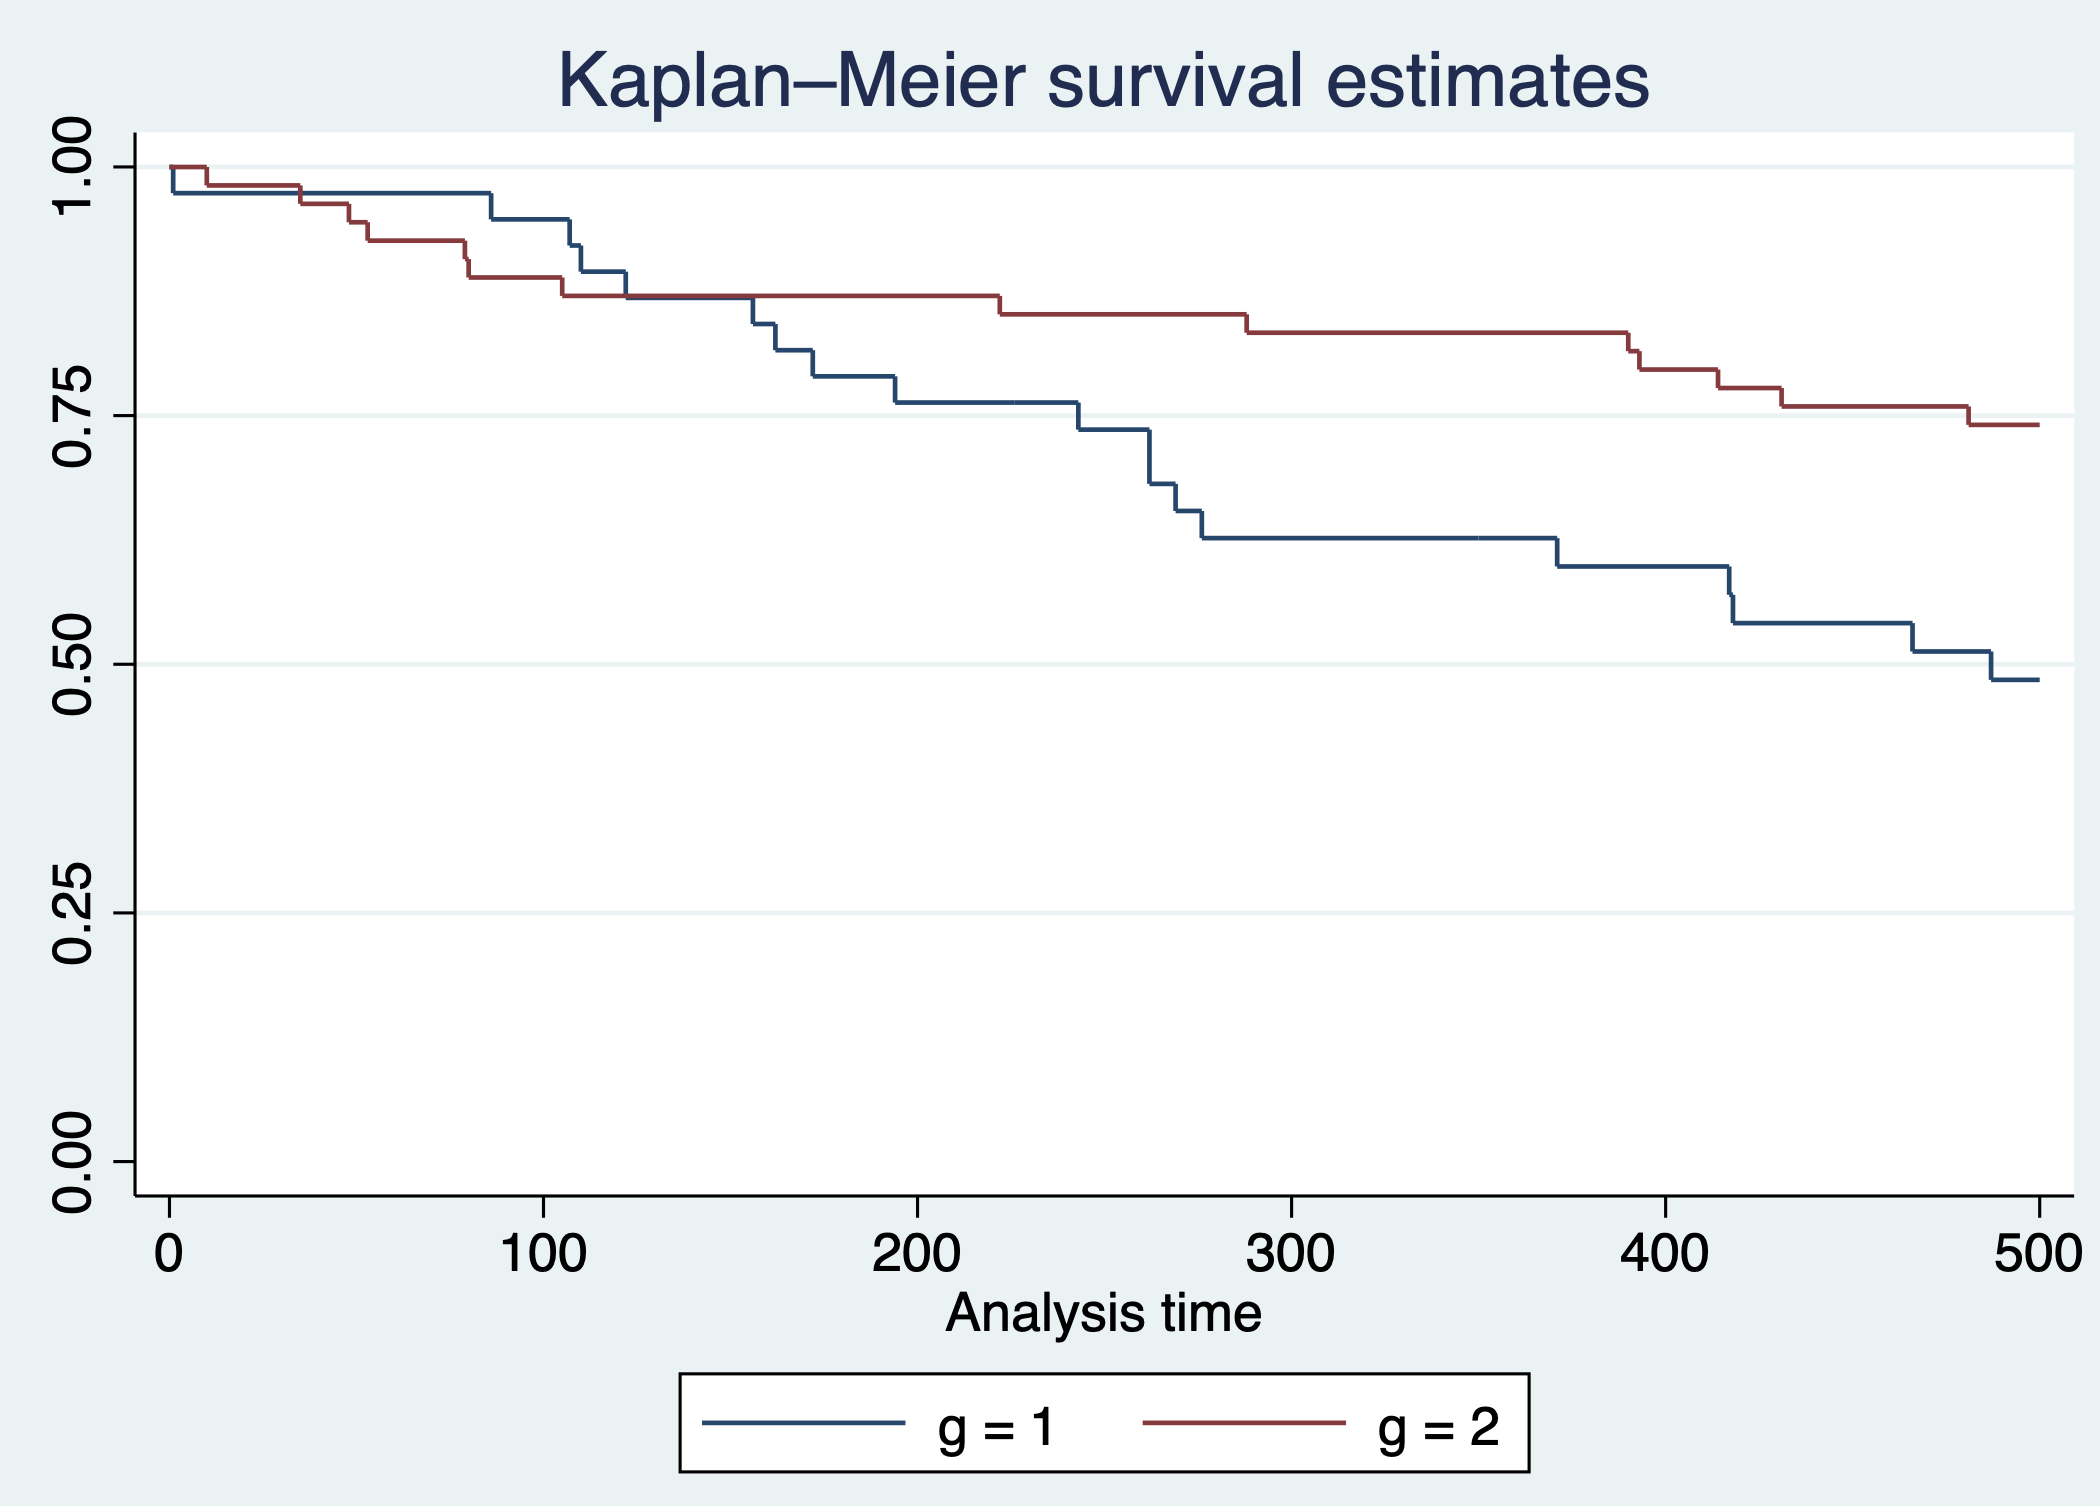
\includegraphics[width=1\linewidth,height=\textheight,keepaspectratio]{chapters/images/ch5-image1.png}

\textbf{代码5.1输出：两组Kaplan-Meier曲线}

第二种方法绘制
Schoenfeld残差与时间的关系图，如果Schoenfeld残差与时间无明显的变化趋势，即残差与时间无关，则提示符合等比例风险假设。如下图中残差似乎有随着时间上升的趋势，提示可能不满足等比例风险假定。

\begin{tcolorbox}[enhanced jigsaw, arc=.35mm, bottomrule=.15mm, breakable, colback=white, colframe=quarto-callout-note-color-frame, left=2mm, leftrule=.75mm, opacityback=0, rightrule=.15mm, toprule=.15mm]

\vspace{-3mm}\textbf{代码5.2}\vspace{3mm}

\begin{Shaded}
\begin{Highlighting}[]
\KeywordTok{stcox}\NormalTok{ g}
\KeywordTok{estat}\NormalTok{ phtest, }\FunctionTok{rank}\NormalTok{ plot(g)}
\end{Highlighting}
\end{Shaded}

\end{tcolorbox}

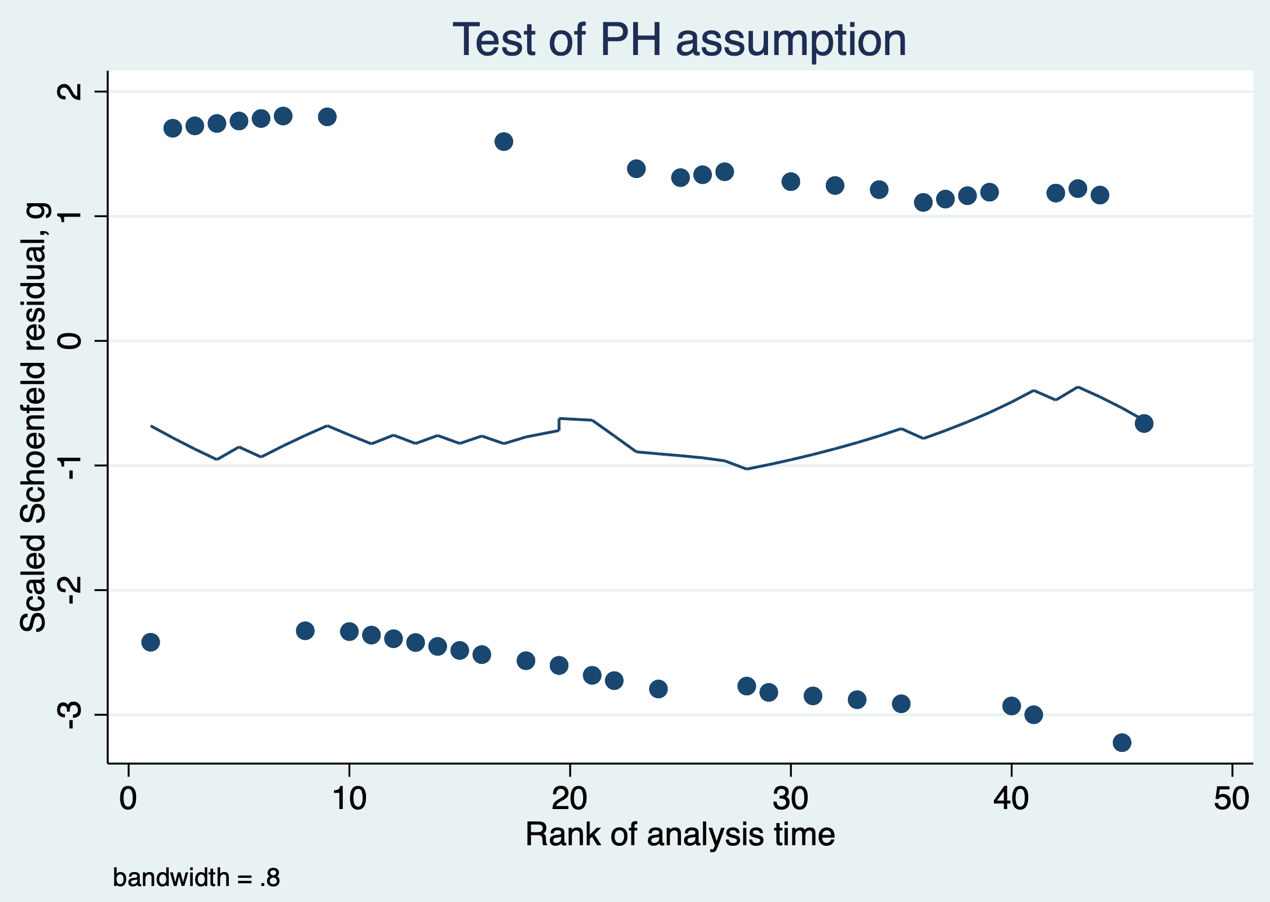
\includegraphics[width=1\linewidth,height=\textheight,keepaspectratio]{chapters/images/ch5-image2.png}

\textbf{代码5.2输出：Schoenfeld残差与时间关系图}

等比例条件的第三个检验方法是绘制某因素在不同状态下的二次对数生存曲线图
（即横坐标是时间的对数，纵坐标是生存函数的对数的对数），如果生存曲线大致平行，表明等比例风险成立，否则提示等比例不成立。如下图中两条曲线交叉，提示可能不满足等比例风险假定。

\begin{tcolorbox}[enhanced jigsaw, arc=.35mm, bottomrule=.15mm, breakable, colback=white, colframe=quarto-callout-note-color-frame, left=2mm, leftrule=.75mm, opacityback=0, rightrule=.15mm, toprule=.15mm]

\vspace{-3mm}\textbf{代码5.3}\vspace{3mm}

\begin{Shaded}
\begin{Highlighting}[]
\KeywordTok{stphplot}\NormalTok{, }\KeywordTok{by}\NormalTok{(g)}
\end{Highlighting}
\end{Shaded}

\end{tcolorbox}

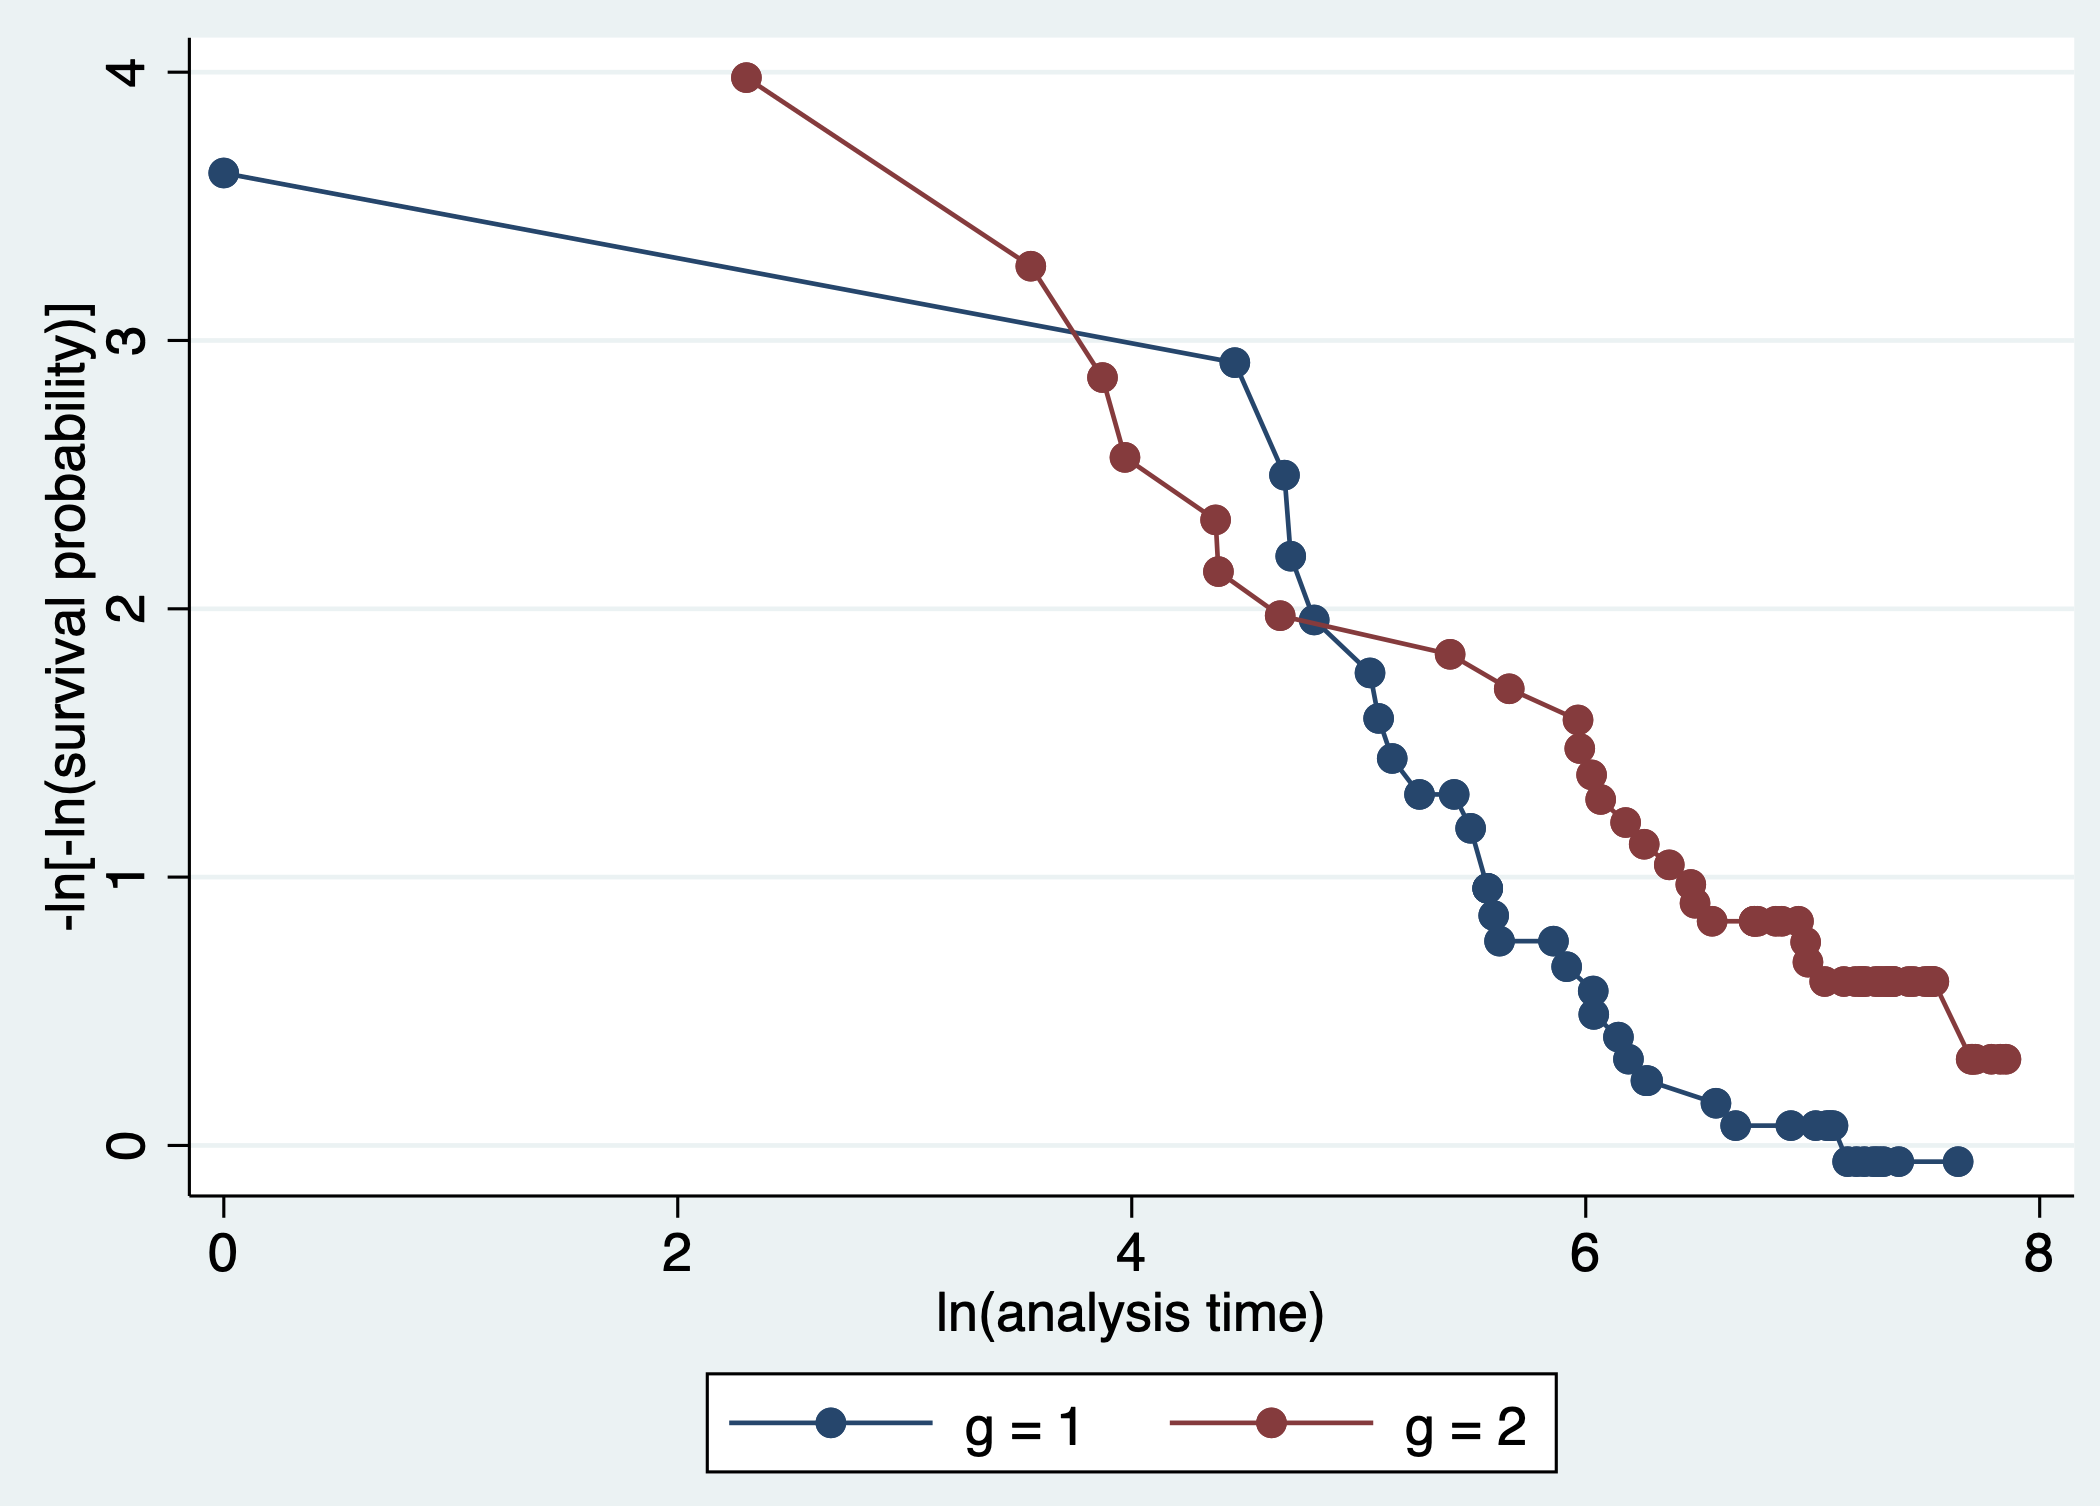
\includegraphics[width=1\linewidth,height=\textheight,keepaspectratio]{chapters/images/ch5-image3.png}

\textbf{代码5.3输出：二次对数生存曲线图}

\subsection{非等比例情况下的Cox回归}\label{ux975eux7b49ux6bd4ux4f8bux60c5ux51b5ux4e0bux7684coxux56deux5f52}

Cox回归模型中，如果数据中存在非等比例的情况，可采用以下三种策略开展生存分析。

\subsection{加速失效时间模型（accelerated failure-time
model，AFT）}\label{ux52a0ux901fux5931ux6548ux65f6ux95f4ux6a21ux578baccelerated-failure-time-modelaft}

主要研究干预对事件发生平均经历的时间的影响。直观上可以理解为比较两种干预结局事件发生的速度。其回归系数表示发生结局事件所需时间的比值，如果结局事件为死亡，回归系数即表示两组平均寿命的比值。

指定生存数据模式后，采用streg命令进行回归分析，随机变量的分布可以选择指数分布、Weibull分布、伽马分布等等。

\begin{tcolorbox}[enhanced jigsaw, arc=.35mm, bottomrule=.15mm, breakable, colback=white, colframe=quarto-callout-note-color-frame, left=2mm, leftrule=.75mm, opacityback=0, rightrule=.15mm, toprule=.15mm]

\vspace{-3mm}\textbf{代码5.4}\vspace{3mm}

\begin{Shaded}
\begin{Highlighting}[]
\KeywordTok{stset}\NormalTok{ t1, failure(delta1==1)}
\KeywordTok{streg}\NormalTok{ g, distribution(exponential) time}
\end{Highlighting}
\end{Shaded}

\end{tcolorbox}

\begin{tcolorbox}[enhanced jigsaw, arc=.35mm, bottomrule=.15mm, breakable, colback=white, colframe=quarto-callout-note-color-frame, left=2mm, leftrule=.75mm, opacityback=0, rightrule=.15mm, toprule=.15mm]

\vspace{-3mm}\textbf{代码5.4输出}\vspace{3mm}

{\def\LTcaptype{none} % do not increment counter
\begin{longtable}[]{@{}
  >{\raggedright\arraybackslash}p{(\linewidth - 12\tabcolsep) * \real{0.1429}}
  >{\raggedright\arraybackslash}p{(\linewidth - 12\tabcolsep) * \real{0.1429}}
  >{\raggedright\arraybackslash}p{(\linewidth - 12\tabcolsep) * \real{0.1429}}
  >{\raggedright\arraybackslash}p{(\linewidth - 12\tabcolsep) * \real{0.1429}}
  >{\raggedright\arraybackslash}p{(\linewidth - 12\tabcolsep) * \real{0.1429}}
  >{\raggedright\arraybackslash}p{(\linewidth - 12\tabcolsep) * \real{0.1429}}
  >{\raggedright\arraybackslash}p{(\linewidth - 12\tabcolsep) * \real{0.1429}}@{}}
\toprule\noalign{}
\begin{minipage}[b]{\linewidth}\raggedright
Exponential AFT regression
\end{minipage} & \begin{minipage}[b]{\linewidth}\raggedright
\end{minipage} & \begin{minipage}[b]{\linewidth}\raggedright
\end{minipage} & \begin{minipage}[b]{\linewidth}\raggedright
\end{minipage} & \begin{minipage}[b]{\linewidth}\raggedright
\end{minipage} & \begin{minipage}[b]{\linewidth}\raggedright
\end{minipage} & \begin{minipage}[b]{\linewidth}\raggedright
\end{minipage} \\
\midrule\noalign{}
\endhead
\bottomrule\noalign{}
\endlastfoot
No.~of subjects = 92 & Number of obs & = & \textbf{92} & & & \\
No.~of failures = 46 & LR chi2(1) & = & \textbf{8.47} & & & \\
Time at risk = 86,200 & Prob \textgreater{} chi2 & = & \textbf{0.0036} &
& & \\
Log likelihood = -135.20674 & & & & & & \\
& Coefficient & Std. Err. & z & P\textgreater\textbar z\textbar{} &
{[}95\% Conf. Interval{]} & \\
g & \textbf{.8714456} & \textbf{.2948839} & \textbf{2.96} &
\textbf{0.003} & \textbf{.2934837} & \textbf{1.449407} \\
\_cons & \textbf{6.136548} & \textbf{.4662524} & \textbf{13.16} &
\textbf{0.000} & \textbf{5.222711} & \textbf{7.050386} \\
\end{longtable}
}

\end{tcolorbox}

g的系数为0.871，表示g=1组发生结局事件所需时间延长(1-0.871)\%=12.9\%。两组的失效曲线（横轴为时间，纵轴为终点事件发生的比例）也可以观察到g=0组发生结局事件的速度更快。

\begin{tcolorbox}[enhanced jigsaw, arc=.35mm, bottomrule=.15mm, breakable, colback=white, colframe=quarto-callout-note-color-frame, left=2mm, leftrule=.75mm, opacityback=0, rightrule=.15mm, toprule=.15mm]

\vspace{-3mm}\textbf{代码5.5}\vspace{3mm}

\begin{Shaded}
\begin{Highlighting}[]
\KeywordTok{stcurve}\NormalTok{, failure }\FunctionTok{at}\NormalTok{(g=(0 1))}
\end{Highlighting}
\end{Shaded}

\end{tcolorbox}

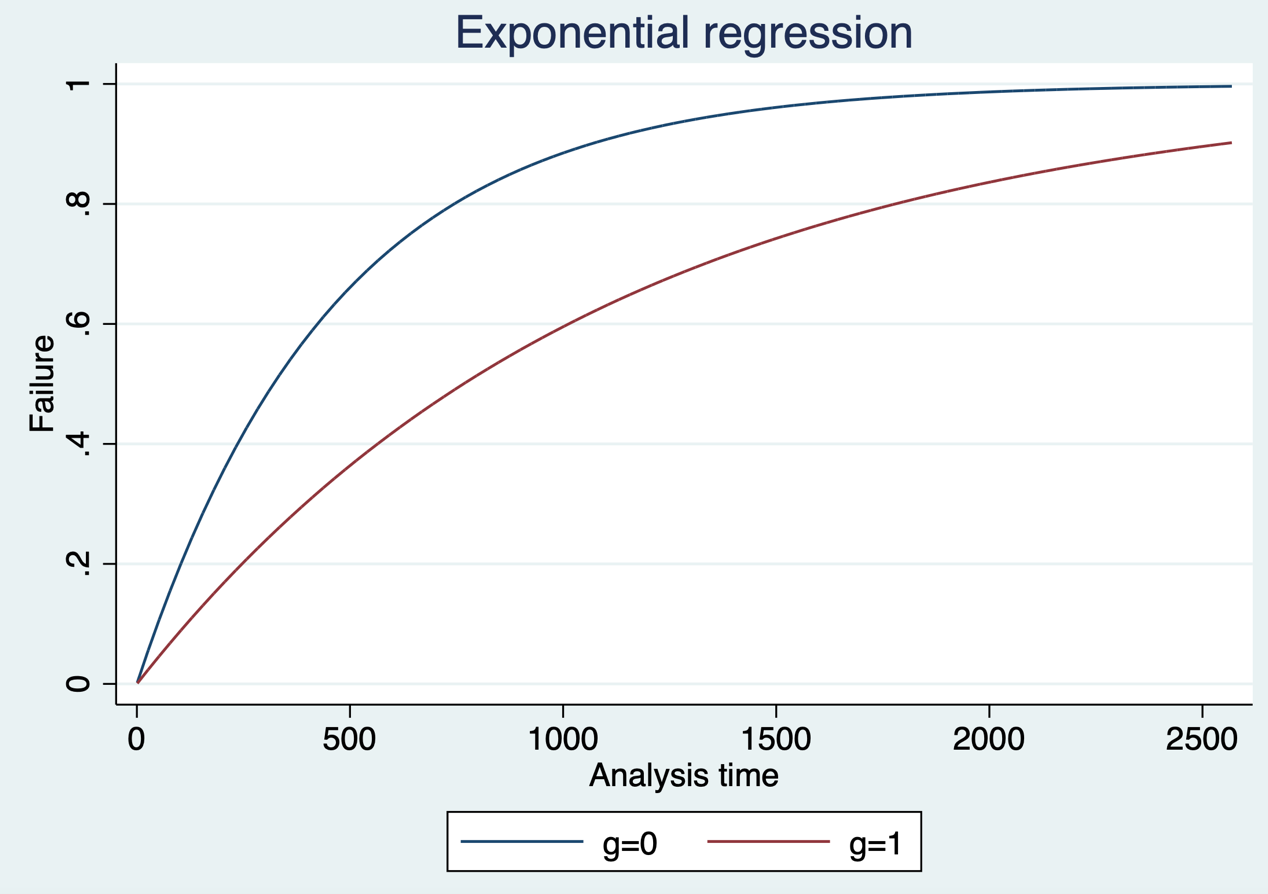
\includegraphics[width=1\linewidth,height=\textheight,keepaspectratio]{chapters/images/ch5-image4.png}

\textbf{代码5.5输出：加速失效曲线图}

\begin{enumerate}
\def\labelenumi{\arabic{enumi}.}
\setcounter{enumi}{1}
\tightlist
\item
  限制性平均生存时间（Restricted mean survival times, RMST）
\end{enumerate}

限制性平均生存时间为生存曲线在某个时间段内的曲线下面积（图5.1粉红色部分），即限制在某个时间段内的平均生存时间。平均生存时间越长，说明治疗的效果越好。限制性平均生存时间是不依赖于等比例风险假设的，其结果也比较直观，容易理解。但计算限制性平均生存时间需确定随访截止时间，但目前对于截止时间没有统一规定，由临床信息给定。

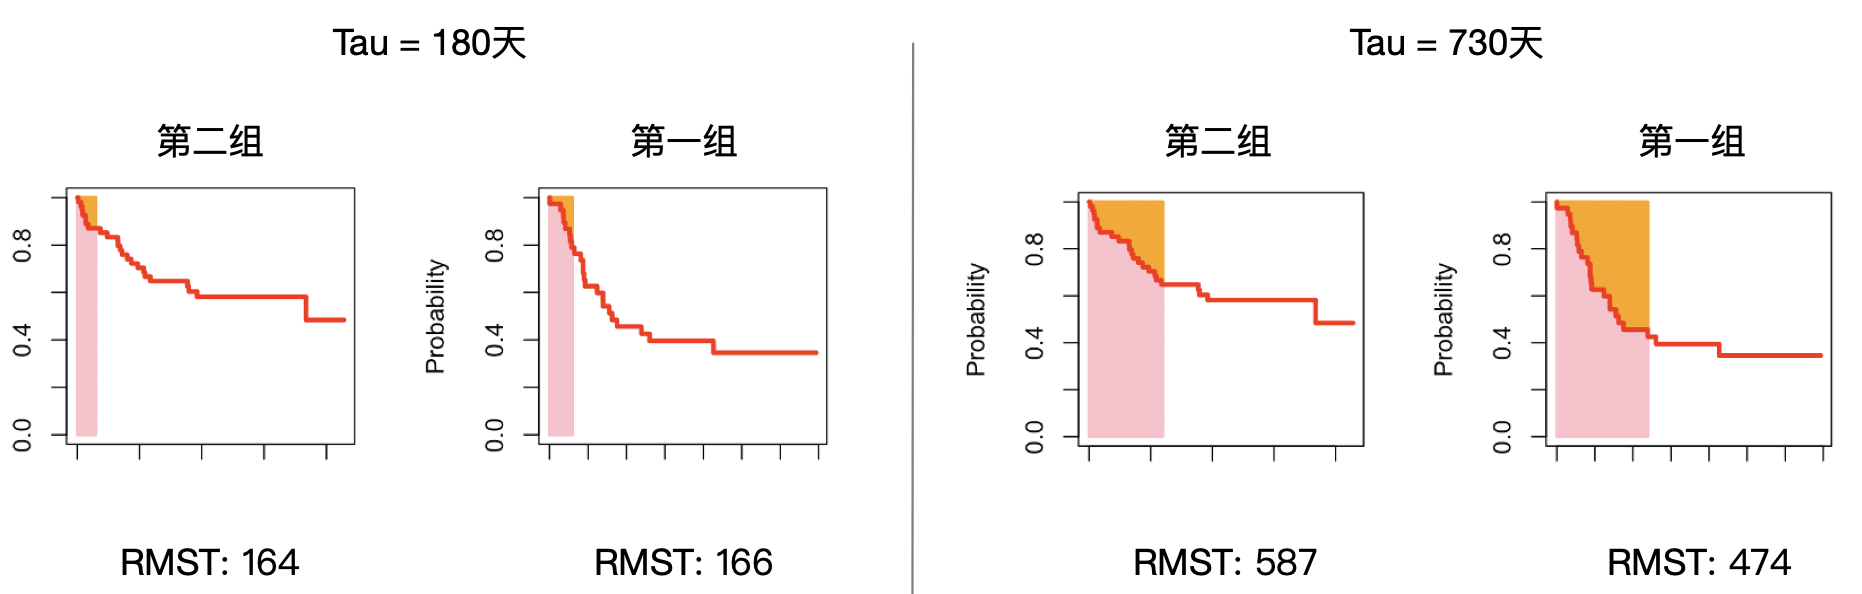
\includegraphics[width=1\linewidth,height=\textheight,keepaspectratio]{chapters/images/ch5-image5.png}

\textbf{图5.1
分别将截止时间定为180天和730天时，两组的限制性平均生存时间}

案例5.1中手术后短期内低风险性的急性髓系白血病死亡风险大于急性淋巴细胞性白血病组可能是由于手术后的急性反应。临床上，这个时间一般持续3个月到半年左右。因此可以将截止时间（tau）定义为180天，分别计算截止至180天时两组的平均生存时间。strmst2命令用于限制性平均生存时间分析，指定分组变量g和截止时间。

\begin{tcolorbox}[enhanced jigsaw, arc=.35mm, bottomrule=.15mm, breakable, colback=white, colframe=quarto-callout-note-color-frame, left=2mm, leftrule=.75mm, opacityback=0, rightrule=.15mm, toprule=.15mm]

\vspace{-3mm}\textbf{代码5.6}\vspace{3mm}

\begin{Shaded}
\begin{Highlighting}[]
\NormalTok{strmst2 g, tau(180)}
\end{Highlighting}
\end{Shaded}

\end{tcolorbox}

\begin{tcolorbox}[enhanced jigsaw, arc=.35mm, bottomrule=.15mm, breakable, colback=white, colframe=quarto-callout-note-color-frame, left=2mm, leftrule=.75mm, opacityback=0, rightrule=.15mm, toprule=.15mm]

\vspace{-3mm}\textbf{代码5.6输出}\vspace{3mm}

{\def\LTcaptype{none} % do not increment counter
\begin{longtable}[]{@{}
  >{\raggedright\arraybackslash}p{(\linewidth - 8\tabcolsep) * \real{0.2000}}
  >{\raggedright\arraybackslash}p{(\linewidth - 8\tabcolsep) * \real{0.2000}}
  >{\raggedright\arraybackslash}p{(\linewidth - 8\tabcolsep) * \real{0.2000}}
  >{\raggedright\arraybackslash}p{(\linewidth - 8\tabcolsep) * \real{0.2000}}
  >{\raggedright\arraybackslash}p{(\linewidth - 8\tabcolsep) * \real{0.2000}}@{}}
\toprule\noalign{}
\begin{minipage}[b]{\linewidth}\raggedright
Restricted Mean Survival Time (RMST) by arm
\end{minipage} & \begin{minipage}[b]{\linewidth}\raggedright
\end{minipage} & \begin{minipage}[b]{\linewidth}\raggedright
\end{minipage} & \begin{minipage}[b]{\linewidth}\raggedright
\end{minipage} & \begin{minipage}[b]{\linewidth}\raggedright
\end{minipage} \\
\midrule\noalign{}
\endhead
\bottomrule\noalign{}
\endlastfoot
& Estimate & Std. Err. & {[}95\% Conf. Interval{]} & \\
arm2 & \textbf{164.259} & \textbf{5.735} & \textbf{153.018} &
\textbf{175.501} \\
arm1 & \textbf{166.211} & \textbf{5.778} & \textbf{154.886} &
\textbf{177.535} \\
Between-group contrast (arm 2 versus arm 1) & & & & \\
& Estimate & {[}95\% Conf. Interval{]} &
P\textgreater\textbar z\textbar{} & \\
RMST (arm2 - arm1) & \textbf{-1.951} & \textbf{-17.908} &
\textbf{14.005} & \textbf{0.811} \\
RMST (arm2 / arm1) & \textbf{0.988} & \textbf{0.897} & \textbf{1.088} &
\textbf{0.811} \\
\end{longtable}
}

\end{tcolorbox}

180天时第一组的限制性平均生存时间是166天，第二组的限制性平均生存时间是164天，两组之间没有明显的差别（无论是差值还是比值），p值为0.811。如果我们想要比较两组的长期治疗效果，只需将截止时间定为更长的随访（如730天），可看到第一组的限制性平均生存时间是473，第二组的限制性平均生存时间为587，两组相比差值的p值为0.035，比值的p值为0.042。可以得出结论截止730天时，第一组患者的限制性平均生存时间比第二组短。

\begin{tcolorbox}[enhanced jigsaw, arc=.35mm, bottomrule=.15mm, breakable, colback=white, colframe=quarto-callout-note-color-frame, left=2mm, leftrule=.75mm, opacityback=0, rightrule=.15mm, toprule=.15mm]

\vspace{-3mm}\textbf{代码5.7}\vspace{3mm}

\begin{Shaded}
\begin{Highlighting}[]
\NormalTok{strmst2 g, tau(730)}
\end{Highlighting}
\end{Shaded}

\end{tcolorbox}

\begin{tcolorbox}[enhanced jigsaw, arc=.35mm, bottomrule=.15mm, breakable, colback=white, colframe=quarto-callout-note-color-frame, left=2mm, leftrule=.75mm, opacityback=0, rightrule=.15mm, toprule=.15mm]

\vspace{-3mm}\textbf{代码5.7输出}\vspace{3mm}

{\def\LTcaptype{none} % do not increment counter
\begin{longtable}[]{@{}
  >{\raggedright\arraybackslash}p{(\linewidth - 8\tabcolsep) * \real{0.2000}}
  >{\raggedright\arraybackslash}p{(\linewidth - 8\tabcolsep) * \real{0.2000}}
  >{\raggedright\arraybackslash}p{(\linewidth - 8\tabcolsep) * \real{0.2000}}
  >{\raggedright\arraybackslash}p{(\linewidth - 8\tabcolsep) * \real{0.2000}}
  >{\raggedright\arraybackslash}p{(\linewidth - 8\tabcolsep) * \real{0.2000}}@{}}
\toprule\noalign{}
\begin{minipage}[b]{\linewidth}\raggedright
Restricted Mean Survival Time (RMST) by arm
\end{minipage} & \begin{minipage}[b]{\linewidth}\raggedright
\end{minipage} & \begin{minipage}[b]{\linewidth}\raggedright
\end{minipage} & \begin{minipage}[b]{\linewidth}\raggedright
\end{minipage} & \begin{minipage}[b]{\linewidth}\raggedright
\end{minipage} \\
\midrule\noalign{}
\endhead
\bottomrule\noalign{}
\endlastfoot
& Estimate & Std. Err. & {[}95\% Conf. Interval{]} & \\
arm2 & \textbf{586.704} & \textbf{32.427} & \textbf{523.148} &
\textbf{650.260} \\
arm1 & \textbf{473.868} & \textbf{42.191} & \textbf{391.176} &
\textbf{556.561} \\
Between-group contrast (arm 2 versus arm 1) & & & & \\
& Estimate & {[}95\% Conf. Interval{]} &
P\textgreater\textbar z\textbar{} & \\
RMST (arm2 - arm1) & \textbf{112.835} & \textbf{8.540} &
\textbf{217.130} & \textbf{0.034} \\
RMST (arm2 / arm1) & \textbf{1.238} & \textbf{1.008} & \textbf{1.520} &
\textbf{0.042} \\
\end{longtable}
}

\end{tcolorbox}

然而，限制性平均生存时间分析的一个重要弊端在于截止时间点后收集的数据无法用于统计分析，造成了数据的浪费和统计效能下降。作为危险比的替代效应指标，限制性平均生存时间在存在非比例风险时尤为适用，其在随机试验设计与分析中的应用可参见
Royston 与 Parmar（2013）。

\subsection{Landmark分析}\label{landmarkux5206ux6790}

除了限制性平均生存时间，存在非等比例情况下亦可以使用Landmark分析，其原理是把
Kaplan-Meier
曲线分成两段，前面一段和后面一段分别做Cox模型分析。Landmark分析考虑到两个干预组发生终点事件的时间分布不同。如果要比较某种疾病手术组和非手术组的生存率，因为手术组短期有相对较高的并发症率，导致短期生存率低于对照组，但一旦过了这个时期，手术组的生存率可能大于非手术组。Landmark
分析通过设定一个地标时间点、仅纳入在该时点仍存活的受试者，避免了用尚未发生的信息进行不当比较，其方法学可参见
Dafni（2011）。

同样采用案例5.1，Kaplan-Meier
曲线可以看到第二组的长期预后较好，但在术后短期存在生存率的快速下降。因此，我们想要知道术后短期内两组的生存情况有何差别，术后长期的情况又是如何？

Landmark
分析的步骤为基于临床经验选择Landmark时间，分别在Landmark时间前后进行Cox回归分析。在案例5.1中，急性反应一般发生于手术后180天，首先计算180天内两组的生存函数差别，需手工截断尚未发生生存事件的患者的生存时间至180天。结果提示两组生存函数无明显差别（p=0.373）。

\begin{tcolorbox}[enhanced jigsaw, arc=.35mm, bottomrule=.15mm, breakable, colback=white, colframe=quarto-callout-note-color-frame, left=2mm, leftrule=.75mm, opacityback=0, rightrule=.15mm, toprule=.15mm]

\vspace{-3mm}\textbf{代码5.8}\vspace{3mm}

\begin{Shaded}
\begin{Highlighting}[]
\KeywordTok{gen}\NormalTok{ L1 = t1 }\KeywordTok{if}\NormalTok{ t1 \textless{} 180}
\KeywordTok{replace}\NormalTok{ L1 = 180 }\KeywordTok{if}\NormalTok{ t1 \textgreater{}= 180}
\KeywordTok{gen}\NormalTok{ deltaL1 = delta1 }\KeywordTok{if}\NormalTok{ t1 \textless{} 180}
\KeywordTok{replace}\NormalTok{ deltaL1 = 0 }\KeywordTok{if}\NormalTok{ t1 \textgreater{}= 180}
\KeywordTok{stset}\NormalTok{ L1, failure(deltaL1==1)}
\KeywordTok{stcox}\NormalTok{ g}
\end{Highlighting}
\end{Shaded}

\end{tcolorbox}

\begin{tcolorbox}[enhanced jigsaw, arc=.35mm, bottomrule=.15mm, breakable, colback=white, colframe=quarto-callout-note-color-frame, left=2mm, leftrule=.75mm, opacityback=0, rightrule=.15mm, toprule=.15mm]

\vspace{-3mm}\textbf{代码5.8输出}\vspace{3mm}

{\def\LTcaptype{none} % do not increment counter
\begin{longtable}[]{@{}
  >{\raggedright\arraybackslash}p{(\linewidth - 12\tabcolsep) * \real{0.1429}}
  >{\raggedright\arraybackslash}p{(\linewidth - 12\tabcolsep) * \real{0.1429}}
  >{\raggedright\arraybackslash}p{(\linewidth - 12\tabcolsep) * \real{0.1429}}
  >{\raggedright\arraybackslash}p{(\linewidth - 12\tabcolsep) * \real{0.1429}}
  >{\raggedright\arraybackslash}p{(\linewidth - 12\tabcolsep) * \real{0.1429}}
  >{\raggedright\arraybackslash}p{(\linewidth - 12\tabcolsep) * \real{0.1429}}
  >{\raggedright\arraybackslash}p{(\linewidth - 12\tabcolsep) * \real{0.1429}}@{}}
\toprule\noalign{}
\begin{minipage}[b]{\linewidth}\raggedright
Cox regression with no ties
\end{minipage} & \begin{minipage}[b]{\linewidth}\raggedright
\end{minipage} & \begin{minipage}[b]{\linewidth}\raggedright
\end{minipage} & \begin{minipage}[b]{\linewidth}\raggedright
\end{minipage} & \begin{minipage}[b]{\linewidth}\raggedright
\end{minipage} & \begin{minipage}[b]{\linewidth}\raggedright
\end{minipage} & \begin{minipage}[b]{\linewidth}\raggedright
\end{minipage} \\
\midrule\noalign{}
\endhead
\bottomrule\noalign{}
\endlastfoot
No.~of subjects = 92 & Number of obs & = & \textbf{92} & & & \\
No.~of failures = 15 & LR chi2(1) & = & \textbf{0.80} & & & \\
Time at risk = 15,186 & Prob \textgreater{} chi2 & = & \textbf{0.3723} &
& & \\
Log likelihood = -66.222312 & & & & & & \\
& Haz.ratio & Std. Err. & z & P\textgreater\textbar z\textbar{} &
{[}95\% Conf. Interval{]} & \\
g & \textbf{.630299} & \textbf{.3263916} & \textbf{-0.89} &
\textbf{0.373} & \textbf{.2285066} & \textbf{1.738579} \\
\end{longtable}
}

\end{tcolorbox}

然后计算手术180天后两组的生存函数差别，删除生存时间小于180天的受试者，从180天开始重新计算随访时间。结果提示手术180天后，急性淋巴细胞性白血病的生存率（蓝色曲线）较低风险性的急性髓系白血病生存率（红色曲线）低。

\begin{tcolorbox}[enhanced jigsaw, arc=.35mm, bottomrule=.15mm, breakable, colback=white, colframe=quarto-callout-note-color-frame, left=2mm, leftrule=.75mm, opacityback=0, rightrule=.15mm, toprule=.15mm]

\vspace{-3mm}\textbf{代码5.9}\vspace{3mm}

\begin{Shaded}
\begin{Highlighting}[]
\KeywordTok{gen}\NormalTok{ L2 = t1 {-} 180}
\KeywordTok{stset}\NormalTok{ L2, failure(delta1==1)}
\KeywordTok{stcox}\NormalTok{ g }\KeywordTok{if}\NormalTok{ L2 \textgreater{} 0}
\KeywordTok{sts} \KeywordTok{graph} \KeywordTok{if}\NormalTok{ L2 \textgreater{} 0, }\KeywordTok{by}\NormalTok{(g) risktable censored(single)}
\end{Highlighting}
\end{Shaded}

\end{tcolorbox}

\begin{tcolorbox}[enhanced jigsaw, arc=.35mm, bottomrule=.15mm, breakable, colback=white, colframe=quarto-callout-note-color-frame, left=2mm, leftrule=.75mm, opacityback=0, rightrule=.15mm, toprule=.15mm]

\vspace{-3mm}\textbf{代码5.9输出}\vspace{3mm}

{\def\LTcaptype{none} % do not increment counter
\begin{longtable}[]{@{}
  >{\raggedright\arraybackslash}p{(\linewidth - 12\tabcolsep) * \real{0.1429}}
  >{\raggedright\arraybackslash}p{(\linewidth - 12\tabcolsep) * \real{0.1429}}
  >{\raggedright\arraybackslash}p{(\linewidth - 12\tabcolsep) * \real{0.1429}}
  >{\raggedright\arraybackslash}p{(\linewidth - 12\tabcolsep) * \real{0.1429}}
  >{\raggedright\arraybackslash}p{(\linewidth - 12\tabcolsep) * \real{0.1429}}
  >{\raggedright\arraybackslash}p{(\linewidth - 12\tabcolsep) * \real{0.1429}}
  >{\raggedright\arraybackslash}p{(\linewidth - 12\tabcolsep) * \real{0.1429}}@{}}
\toprule\noalign{}
\begin{minipage}[b]{\linewidth}\raggedright
Cox regression with Breslow method for ties
\end{minipage} & \begin{minipage}[b]{\linewidth}\raggedright
\end{minipage} & \begin{minipage}[b]{\linewidth}\raggedright
\end{minipage} & \begin{minipage}[b]{\linewidth}\raggedright
\end{minipage} & \begin{minipage}[b]{\linewidth}\raggedright
\end{minipage} & \begin{minipage}[b]{\linewidth}\raggedright
\end{minipage} & \begin{minipage}[b]{\linewidth}\raggedright
\end{minipage} \\
\midrule\noalign{}
\endhead
\bottomrule\noalign{}
\endlastfoot
No.~of subjects = 77 & Number of obs & = & \textbf{77} & & & \\
No.~of failures = 31 & LR chi2(1) & = & \textbf{4.24} & & & \\
Time at risk = 84,874 & Prob \textgreater{} chi2 & = & \textbf{0.0395} &
& & \\
Log likelihood = -121.57006 & & & & & & \\
& Haz.ratio & Std. Err. & z & P\textgreater\textbar z\textbar{} &
{[}95\% Conf. Interval{]} & \\
g & \textbf{.466382} & \textbf{.1708153} & \textbf{-2.08} &
\textbf{0.037} & \textbf{.2275014} & \textbf{0.9560918} \\
\end{longtable}
}

\end{tcolorbox}

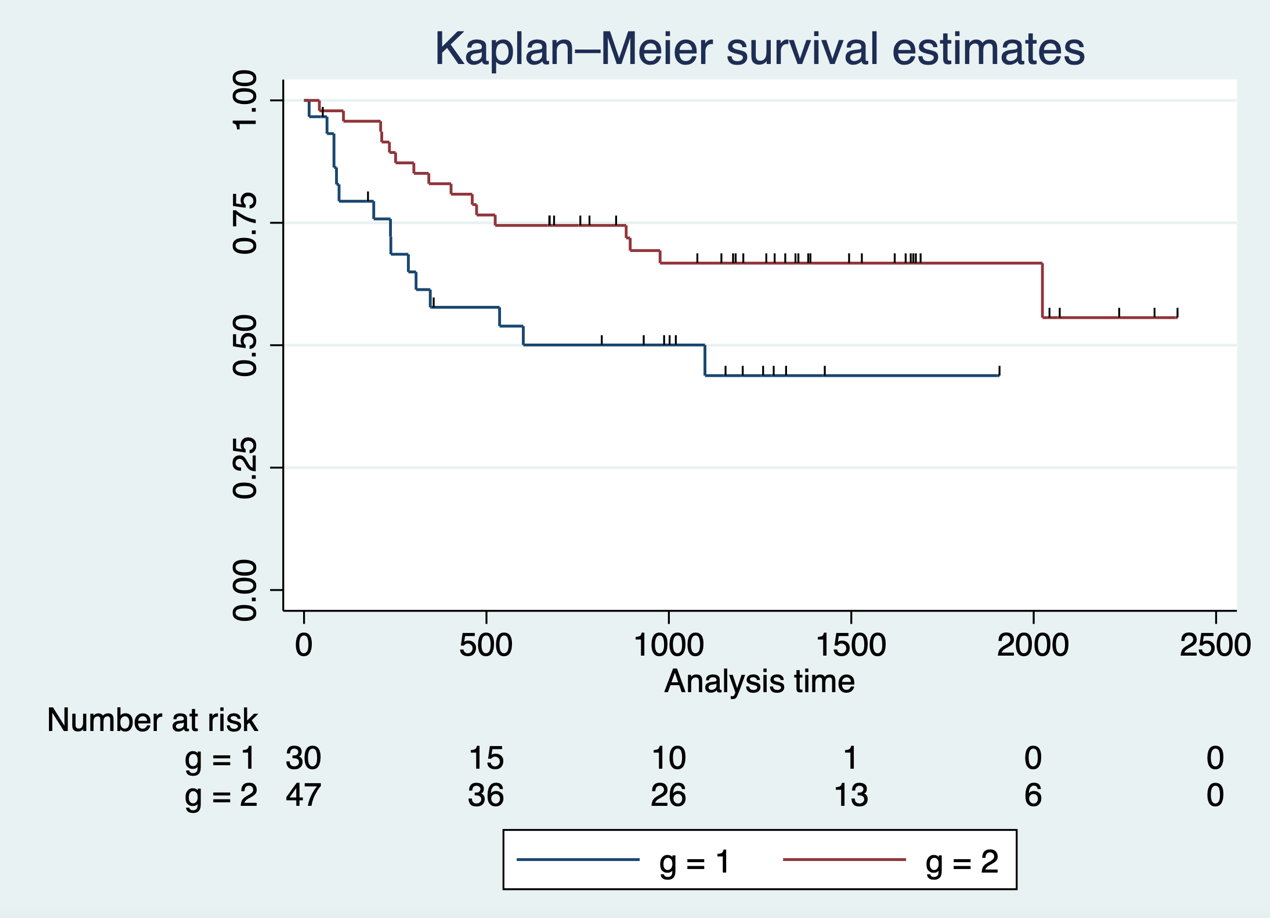
\includegraphics[width=1\linewidth,height=\textheight,keepaspectratio]{chapters/images/ch5-image6.png}

\textbf{代码5.9输出：180天后两组Kaplan-Meier曲线}

总结一下等比例条件满足与不满足情况下的Cox回归分析方法。等比例Cox分析是最常用的Cox分析方法，统计学假设是在不同时间点上，各个组之间的风险比例是相等的。而限制性生存时间分析和Landmark分析都不需要等比例假设，限制性生存时间分析方法指定截止时间，计算截止时间之前的两条生存曲线下的面积，通过比较面积来评估生存曲线差异。Landmark分析则是指定Landmark时间，比较Landmark时间前后的生存曲线差异（图5.2）。

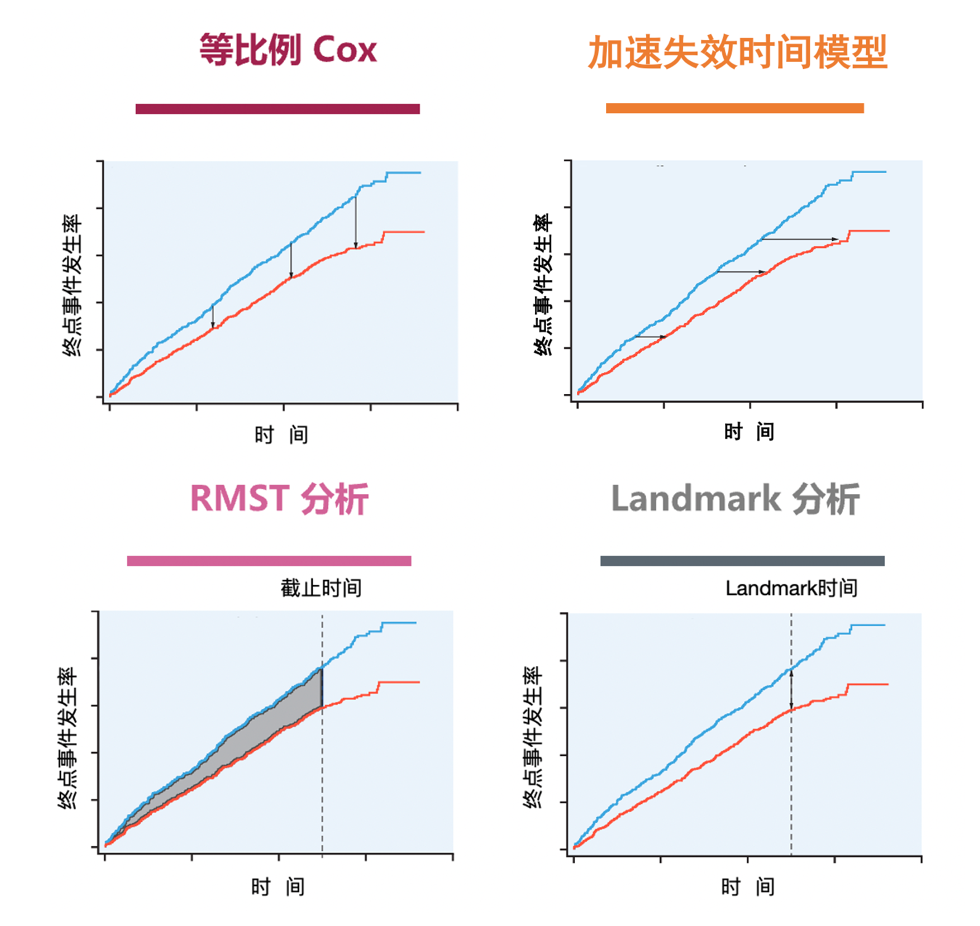
\includegraphics[width=1\linewidth,height=\textheight,keepaspectratio]{chapters/images/ch5-image7.png}

\textbf{图5.2 生存分析除Cox模型外的几种选择}

临床试验中对等比例进行事后分析，有时可以提供有用的见解。第一步是评估等比例假设是否合理。对等比例的正式统计测试有时是有用的，然而多数情况下，在样本量较小的研究中可能会错过临床上重要的偏离等比例的情况，而在样本量较大的研究中却可能会发现临床上不重要的偏离等比例的情况。因此，图形显示，包括Kaplan-Meier曲线和Schoenfeld
残差图可能更有用。

当等比例假设不成立时，使用分段风险模型（类似landmark分析，将随访时间分为若干小段，分别计算小段中的危险比）可能是有用的。这种方法的一个局限性是事后选择不同的时间段，可能会夸大危险比随时间变化的实际差异。随访后期计算出的危险比只包括幸存者（删失了死亡的患者），所以不是真正的随机比较。

另一个事后分析是探讨非等比例是否是由临床上不同的亚组造成的，这些病人的治疗效果是不同的。在这种情况下，亚组分析或分层的Cox模型可能是有用的。此外，在研究进行过程中，受试者脱离原本的分配治疗或交叉至另一组也可能导致非等比例，因为治疗组间随着时间的推移变得更加相似。这对非劣效性试验来说是一个特别的问题，因为治疗效果的稀释可能会导致非劣效性的错误声明。在这种情况下，使用符合方案分析方法，对不依从和交叉的受试者进行统计调整（即计算依从者中的平均因果效应）可能有助于恢复真实治疗效果。非劣效试验的另一个问题是，当非劣效边际是基于危险比的，但比例风险（PH）假设显然不成立。在这种情况下，非劣效边际可能变得不合适或难以解释，因此探索其他分析策略很重要。

\section{含时间依赖变量的Cox回归}\label{ux542bux65f6ux95f4ux4f9dux8d56ux53d8ux91cfux7684coxux56deux5f52}

常规的Cox回归只能研究基线指标与生存结局之间的关系。然而，很多情况下，基线变量可以随着时间变动而发生变动。如，研究吸烟与癌症的发生风险，吸烟状况可以是持续的也可以是不断变化的。基线吸烟后也可以戒烟，戒烟之后又可以再次复吸。同样在脓毒症患者中研究C反应蛋白与死亡率之间的关系，C反应蛋白这个指标也是会随着病情改变而改变的。

这些研究不适用限制性生存时间分析分析或是Landmark分析，因为变量是随着时间变动的；亦或者没有明显的截止时间或者Landmark时间可以采用；又或者如果采用Landmark分析的话可能会导致很多受试者被剔除。

\textbf{案例5.2}

这是一个脓毒症患者中研究C反应蛋白与死亡率之间关系的案例。左表是100例脓毒症患者的临床指标，id表示受试者的唯一识别号；status表示结局事件是死亡或者严重并发症的复合结局事件；start和stop表示基线和结局事件发生的时间（单位为小时）；age表示年龄。右表是这些受试者入院后不同时间点的C反应蛋白值，以id标识唯一识别号；time表示C反应蛋白测定的时间；crp是C反应蛋白测定的值。

\textbf{案例5.2数据表}

{\def\LTcaptype{none} % do not increment counter
\begin{longtable}[]{@{}lllllllll@{}}
\toprule\noalign{}
id & status & start & stop & age & & id & time & crp \\
\midrule\noalign{}
\endhead
\bottomrule\noalign{}
\endlastfoot
1 & 1 & 0 & 48.1 & 80.4 & & 1 & 0 & 110.1 \\
2 & 0 & 0 & 121.4 & 86.1 & & 1 & 189 & 98.9 \\
3 & 1 & 0 & 30.7 & 72.4 & & 1 & 218 & 98.3 \\
4 & 0 & 0 & 500 & 92.0 & & 1 & 230 & 154.7 \\
5 & 1 & 0 & 69.5 & 77.1 & & 2 & 0 & 91 \\
6 & 1 & 0 & 233.1 & 86.8 & & 2 & 27 & 160.7 \\
7 & 1 & 0 & 156.3 & 59.8 & & 2 & 31 & 38 \\
8 & 1 & 0 & 257.6 & 65.6 & & 2 & 114 & 123.4 \\
\ldots{} & \ldots{} & \ldots{} & \ldots{} & \ldots{} & & \ldots{} &
\ldots{} & \ldots{} \\
\end{longtable}
}

在进行数据分析前首先要通过数据格式转化，新建一个数据表，每一行代表每一个感兴趣变量的变化。第一个患者（ID=1）由于在终点事件时间窗内只有一次C反应蛋白的记录，因此在新数据表中只需记录这个患者的一条信息。然而第二个患者（ID=2），由于在终点事件的时间范围内存在很多C反应蛋白的测量值，因此要复制多份记录以存储不同时间的C反应蛋白变化。该患者第一次C反应蛋白的测量时间点为0，终点事件时间点为27（因为下一次C反应蛋白的测量时间点为27），此时尚未发生终点事件。该患者第二次C反应蛋白的测量时间点为27，终点事件时间点为31（因为下一次C反应蛋白的测量时间点为31），此时亦尚未发生终点事件。以此类推，该患者发生终点事件的时间点为121.4，因此新数据表中最后一次C反应蛋白的测量时间点为118（121.4之前的最后一次C反应蛋白测量）。

\textbf{案例5.2数据表转化}

{\def\LTcaptype{none} % do not increment counter
\begin{longtable}[]{@{}lllllllll@{}}
\toprule\noalign{}
id & status & start & stop & age & tstart & tstop & endpt & crp \\
\midrule\noalign{}
\endhead
\bottomrule\noalign{}
\endlastfoot
1 & 1 & 0 & 48.1 & 80.4 & 0 & 48.1 & 1 & 110.1 \\
2 & 0 & 0 & 121.4 & 86.1 & 0 & 27 & 0 & 91 \\
2 & 0 & 0 & 121.4 & 86.1 & 27 & 31 & 0 & 160.7 \\
2 & 0 & 0 & 121.4 & 86.1 & 31 & 114 & 0 & 38 \\
2 & 0 & 0 & 121.4 & 86.1 & 114 & 116 & 0 & 123.4 \\
2 & 0 & 0 & 121.4 & 86.1 & 116 & 118 & 0 & 105 \\
2 & 0 & 0 & 121.4 & 86.1 & 118 & 121.4 & 0 & 108.6 \\
\ldots{} & \ldots{} & \ldots{} & \ldots{} & \ldots{} & \ldots{} &
\ldots{} & \ldots{} & \ldots{} \\
\end{longtable}
}

在重构的新数据中即可进行Cox回归分析，由于数据中有很多受试者被重复计算了多次，因此需要指定哪些受试者是重复的（采用cluster命令）。Cox回归模型p值是0.040，提示C反应蛋白与死亡或者严重并发症的复合结局事件相关。

\begin{tcolorbox}[enhanced jigsaw, arc=.35mm, bottomrule=.15mm, breakable, colback=white, colframe=quarto-callout-note-color-frame, left=2mm, leftrule=.75mm, opacityback=0, rightrule=.15mm, toprule=.15mm]

\vspace{-3mm}\textbf{代码5.10}\vspace{3mm}

\begin{Shaded}
\begin{Highlighting}[]
\KeywordTok{gen}\NormalTok{ time = tstop {-} tstart}
\KeywordTok{stset}\NormalTok{ time, failure(endpt == 1)}
\KeywordTok{stcox}\NormalTok{ crp, }\KeywordTok{cluster}\NormalTok{(id)}
\end{Highlighting}
\end{Shaded}

\end{tcolorbox}

\begin{tcolorbox}[enhanced jigsaw, arc=.35mm, bottomrule=.15mm, breakable, colback=white, colframe=quarto-callout-note-color-frame, left=2mm, leftrule=.75mm, opacityback=0, rightrule=.15mm, toprule=.15mm]

\vspace{-3mm}\textbf{代码5.10输出}\vspace{3mm}

{\def\LTcaptype{none} % do not increment counter
\begin{longtable}[]{@{}
  >{\raggedright\arraybackslash}p{(\linewidth - 12\tabcolsep) * \real{0.1429}}
  >{\raggedright\arraybackslash}p{(\linewidth - 12\tabcolsep) * \real{0.1429}}
  >{\raggedright\arraybackslash}p{(\linewidth - 12\tabcolsep) * \real{0.1429}}
  >{\raggedright\arraybackslash}p{(\linewidth - 12\tabcolsep) * \real{0.1429}}
  >{\raggedright\arraybackslash}p{(\linewidth - 12\tabcolsep) * \real{0.1429}}
  >{\raggedright\arraybackslash}p{(\linewidth - 12\tabcolsep) * \real{0.1429}}
  >{\raggedright\arraybackslash}p{(\linewidth - 12\tabcolsep) * \real{0.1429}}@{}}
\toprule\noalign{}
\begin{minipage}[b]{\linewidth}\raggedright
Cox regression with no ties
\end{minipage} & \begin{minipage}[b]{\linewidth}\raggedright
\end{minipage} & \begin{minipage}[b]{\linewidth}\raggedright
\end{minipage} & \begin{minipage}[b]{\linewidth}\raggedright
\end{minipage} & \begin{minipage}[b]{\linewidth}\raggedright
\end{minipage} & \begin{minipage}[b]{\linewidth}\raggedright
\end{minipage} & \begin{minipage}[b]{\linewidth}\raggedright
\end{minipage} \\
\midrule\noalign{}
\endhead
\bottomrule\noalign{}
\endlastfoot
No.~of subjects = 365 & Number of obs & = & \textbf{365} & & & \\
No.~of failures = 67 & LR chi2(1) & = & \textbf{4.23} & & & \\
Time at risk = 24,688.6661 & Prob \textgreater{} chi2 & = &
\textbf{0.0398} & & & \\
Log pseudolikelihood = -328.58628 & & & & & & \\
& Haz.ratio & Std. Err. & z & P\textgreater\textbar z\textbar{} &
{[}95\% Conf. Interval{]} & \\
crp & \textbf{.9942597} & \textbf{.0027837} & \textbf{-2.06} &
\textbf{0.040} & \textbf{.9888187} & \textbf{0.9997306} \\
\end{longtable}
}

\end{tcolorbox}

\section{竞争风险模型（Competing Risk
Model）}\label{ux7adeux4e89ux98ceux9669ux6a21ux578bcompeting-risk-model}

常规的生存结局事件只有两个，死亡或非死亡；复发或非复发。在真实世界中往往存在多个终点事件，称为竞争风险事件：研究中结局事件有多个，某些结局将阻止感兴趣事件的出现或影响其发生的概率，各结局事件形成竞争关系，互为竞争风险事件（图5.3）。如研究糖尿病患者的卒中风险，如果该患者死亡，则无法观察到卒中事件，故死亡是卒中事件的竞争风险。因此在进行Cox回归时需要考虑多种潜在结局的事件存在。

处理竞争风险比较简单的方法即将多个竞争风险综合考虑。如研究糖尿病患者的卒中风险，死亡是卒中事件的竞争风险，可将结局事件定为卒中或死亡，计算糖尿病患者的无卒中生存概率。然而，实际临床过程需要区分不同事件的风险时可采取下面几种方法。竞争风险数据的系统处理------累积发生函数、Fine--Gray
部分分布模型与原因别风险模型之间的区别与选择------可参见 Fine 与
Gray（1999）、Putter 等（2007）以及 Austin 等（2016）。

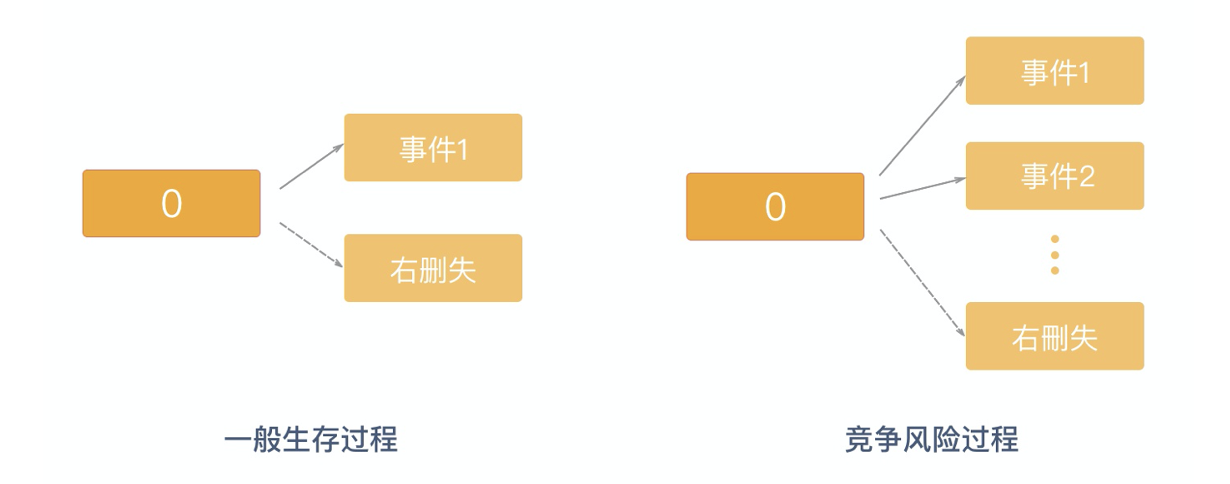
\includegraphics[width=1\linewidth,height=\textheight,keepaspectratio]{chapters/images/ch5-image8.png}

\textbf{图5.3 竞争风险事件}

\textbf{案例5.3}

这是一个黑色素瘤案例，纳入了205例受试者，time指手术以后终点事件的生存时间；status
代表多个感兴趣的结局，1代表黑色素瘤所致的死亡，2代表删失，3代表其他原因所导致的死亡。此结局中黑色素瘤所致的死亡与其他原因所导致的死亡是相互竞争的，因为发生黑色素瘤所产生的死亡就不可能产生其他因素导致的死亡，产生其他因素导致的死亡就不会发生黑色素瘤所产生的死亡。

\textbf{案例5.3数据表}

{\def\LTcaptype{none} % do not increment counter
\begin{longtable}[]{@{}llll@{}}
\toprule\noalign{}
time & status & sex & ulcer \\
\midrule\noalign{}
\endhead
\bottomrule\noalign{}
\endlastfoot
10 & 3 & 1 & 1 \\
30 & 3 & 1 & 0 \\
35 & 2 & 1 & 0 \\
99 & 3 & 0 & 0 \\
185 & 1 & 1 & 1 \\
204 & 1 & 1 & 1 \\
210 & 1 & 1 & 1 \\
\ldots{} & \ldots{} & \ldots{} & \ldots{} \\
\end{longtable}
}

\subsection{累积风险函数（cumulative incidence function,
CIF）}\label{ux7d2fux79efux98ceux9669ux51fdux6570cumulative-incidence-function-cif}

累积风险函数模型描绘感兴趣的结局事件随时间变化率，且考虑了竞争事件的影响。这是一个非参数的模型，用于替代非竞争结局的生存曲线。累积风险模型假设事件每次发生有且仅有一种，具有期望属性，即各类别累积风险之和等于复合事件的累积风险。

指定生存数据时分别指定结局事件为1和3，构建生存曲线时指定采用累积风险模型cif。下图表示黑色素瘤所致死亡以及其他原因所致死亡的累积发生曲线。

\begin{tcolorbox}[enhanced jigsaw, arc=.35mm, bottomrule=.15mm, breakable, colback=white, colframe=quarto-callout-note-color-frame, left=2mm, leftrule=.75mm, opacityback=0, rightrule=.15mm, toprule=.15mm]

\vspace{-3mm}\textbf{代码5.11}\vspace{3mm}

\begin{Shaded}
\begin{Highlighting}[]
\KeywordTok{stset}\NormalTok{ time, fail(status==1)}
\KeywordTok{stcurve}\NormalTok{, cif}
\KeywordTok{stset}\NormalTok{ time, fail(status==3)}
\KeywordTok{stcurve}\NormalTok{, cif}
\end{Highlighting}
\end{Shaded}

\end{tcolorbox}

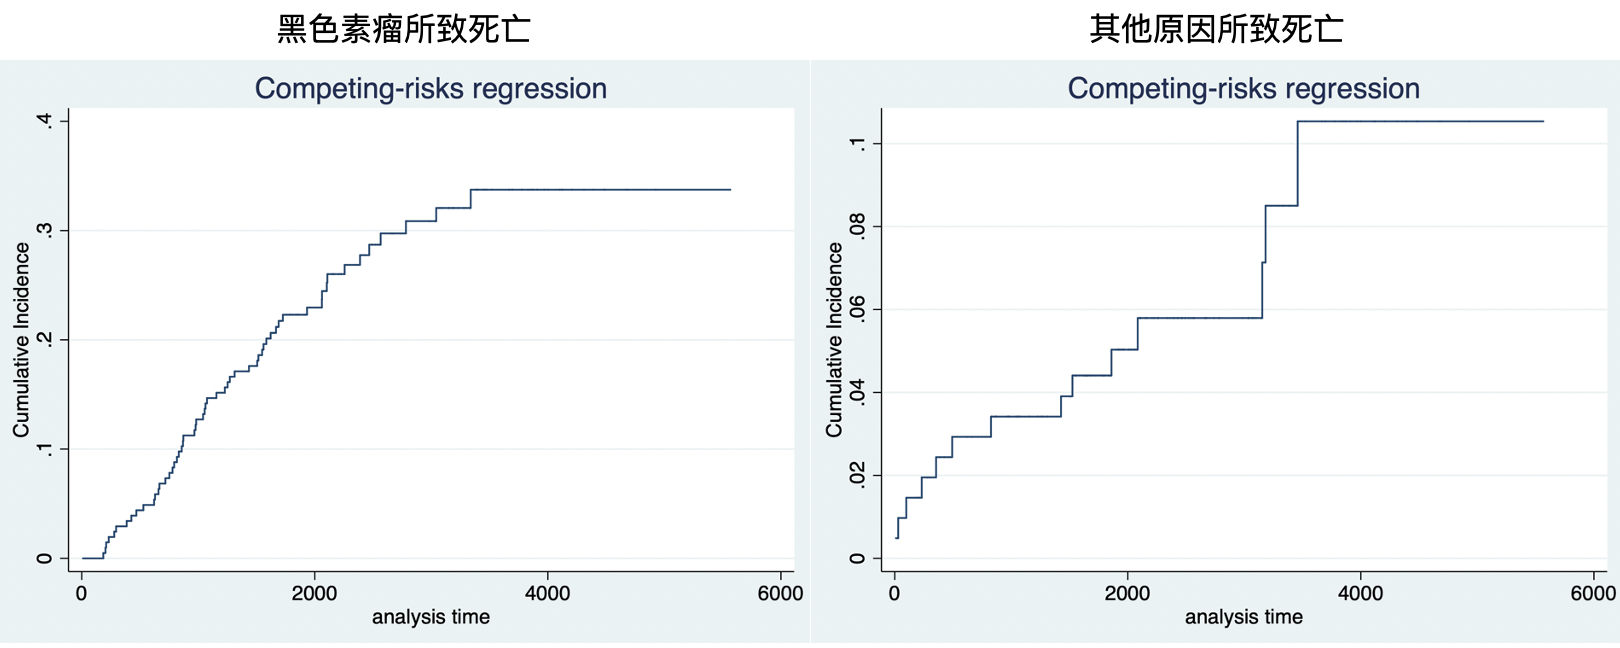
\includegraphics[width=1\linewidth,height=\textheight,keepaspectratio]{chapters/images/ch5-image9.png}

\textbf{代码5.11输出：竞争风险事件的累积风险生存曲线}

\subsection{Fine-Gray模型}\label{fine-grayux6a21ux578b}

Fine-Gray模型是一个半参数的比例风险模型，其定义是指在未发生感兴趣的结局事件的受试者中，感兴趣的结局事件随时间的变化率。可检验感兴趣的结局事件与干预变量的相关性。如我们想要检验有溃疡和没有溃疡的患者因黑色素瘤所致死亡的风险是否一致，即可调用stcrreg命令，结果提示p值\textless0.001，故两组间存在明显差异。作为对照，有溃疡和没有溃疡的患者因其他因素所致死亡的风险一致。Fine-Gray模型采用部分分布比例风险回归，回归系数``SHR''代表部分分布比例风险比。

\begin{tcolorbox}[enhanced jigsaw, arc=.35mm, bottomrule=.15mm, breakable, colback=white, colframe=quarto-callout-note-color-frame, left=2mm, leftrule=.75mm, opacityback=0, rightrule=.15mm, toprule=.15mm]

\vspace{-3mm}\textbf{代码5.12}\vspace{3mm}

\begin{Shaded}
\begin{Highlighting}[]
\KeywordTok{stset}\NormalTok{ time, fail(status == 1)}
\NormalTok{stcrreg ulcer, compete(status == 3)}
\end{Highlighting}
\end{Shaded}

\end{tcolorbox}

\begin{tcolorbox}[enhanced jigsaw, arc=.35mm, bottomrule=.15mm, breakable, colback=white, colframe=quarto-callout-note-color-frame, left=2mm, leftrule=.75mm, opacityback=0, rightrule=.15mm, toprule=.15mm]

\vspace{-3mm}\textbf{代码5.12输出}\vspace{3mm}

{\def\LTcaptype{none} % do not increment counter
\begin{longtable}[]{@{}
  >{\raggedright\arraybackslash}p{(\linewidth - 12\tabcolsep) * \real{0.2609}}
  >{\raggedright\arraybackslash}p{(\linewidth - 12\tabcolsep) * \real{0.1304}}
  >{\raggedright\arraybackslash}p{(\linewidth - 12\tabcolsep) * \real{0.1014}}
  >{\raggedright\arraybackslash}p{(\linewidth - 12\tabcolsep) * \real{0.0942}}
  >{\raggedright\arraybackslash}p{(\linewidth - 12\tabcolsep) * \real{0.0870}}
  >{\raggedright\arraybackslash}p{(\linewidth - 12\tabcolsep) * \real{0.1812}}
  >{\raggedright\arraybackslash}p{(\linewidth - 12\tabcolsep) * \real{0.1087}}@{}}
\toprule\noalign{}
\begin{minipage}[b]{\linewidth}\raggedright
Competing-risks regression
\end{minipage} & \begin{minipage}[b]{\linewidth}\raggedright
No.~of obs
\end{minipage} & \begin{minipage}[b]{\linewidth}\raggedright
=
\end{minipage} & \begin{minipage}[b]{\linewidth}\raggedright
\textbf{205}
\end{minipage} & \begin{minipage}[b]{\linewidth}\raggedright
\end{minipage} & \begin{minipage}[b]{\linewidth}\raggedright
\end{minipage} & \begin{minipage}[b]{\linewidth}\raggedright
\end{minipage} \\
\midrule\noalign{}
\endhead
\bottomrule\noalign{}
\endlastfoot
& No.~of subjects & = & \textbf{205} & & & \\
Failure event: status == 1 & No.~failed & = & \textbf{57} & & & \\
Competing event: status == 3 & No.~competing & = & \textbf{14} & & & \\
& No.~censored & = & \textbf{134} & & & \\
& Wald chi2(1) & = & \textbf{23.91} & & & \\
Log pseudolikelihood = -272.77498 & Prob \textgreater{} chi2 & = &
\textbf{0.0000} & & & \\
& SHR & Robust

std. Err. & z & P\textgreater\textbar z\textbar{} & {[}95\% Conf.
Interval{]} & \\
ulcer & \textbf{4.111191} & \textbf{1.18869} & \textbf{4.89} &
\textbf{0.000} & \textbf{2.332681} & \textbf{7.245693} \\
\end{longtable}
}

\end{tcolorbox}

\begin{tcolorbox}[enhanced jigsaw, arc=.35mm, bottomrule=.15mm, breakable, colback=white, colframe=quarto-callout-note-color-frame, left=2mm, leftrule=.75mm, opacityback=0, rightrule=.15mm, toprule=.15mm]

\vspace{-3mm}\textbf{代码5.13}\vspace{3mm}

\begin{Shaded}
\begin{Highlighting}[]
\KeywordTok{stset}\NormalTok{ time, fail(status == 3)}
\NormalTok{stcrreg ulcer, compete(status == 1)}
\end{Highlighting}
\end{Shaded}

\end{tcolorbox}

\begin{tcolorbox}[enhanced jigsaw, arc=.35mm, bottomrule=.15mm, breakable, colback=white, colframe=quarto-callout-note-color-frame, left=2mm, leftrule=.75mm, opacityback=0, rightrule=.15mm, toprule=.15mm]

\vspace{-3mm}\textbf{代码5.13输出}\vspace{3mm}

{\def\LTcaptype{none} % do not increment counter
\begin{longtable}[]{@{}
  >{\raggedright\arraybackslash}p{(\linewidth - 12\tabcolsep) * \real{0.2571}}
  >{\raggedright\arraybackslash}p{(\linewidth - 12\tabcolsep) * \real{0.1286}}
  >{\raggedright\arraybackslash}p{(\linewidth - 12\tabcolsep) * \real{0.1143}}
  >{\raggedright\arraybackslash}p{(\linewidth - 12\tabcolsep) * \real{0.0929}}
  >{\raggedright\arraybackslash}p{(\linewidth - 12\tabcolsep) * \real{0.0857}}
  >{\raggedright\arraybackslash}p{(\linewidth - 12\tabcolsep) * \real{0.1786}}
  >{\raggedright\arraybackslash}p{(\linewidth - 12\tabcolsep) * \real{0.1071}}@{}}
\toprule\noalign{}
\begin{minipage}[b]{\linewidth}\raggedright
Competing-risks regression
\end{minipage} & \begin{minipage}[b]{\linewidth}\raggedright
No.~of obs
\end{minipage} & \begin{minipage}[b]{\linewidth}\raggedright
=
\end{minipage} & \begin{minipage}[b]{\linewidth}\raggedright
\textbf{205}
\end{minipage} & \begin{minipage}[b]{\linewidth}\raggedright
\end{minipage} & \begin{minipage}[b]{\linewidth}\raggedright
\end{minipage} & \begin{minipage}[b]{\linewidth}\raggedright
\end{minipage} \\
\midrule\noalign{}
\endhead
\bottomrule\noalign{}
\endlastfoot
& No.~of subjects & = & \textbf{205} & & & \\
Failure event: status == 3 & No.~failed & = & \textbf{14} & & & \\
Competing event: status == 1 & No.~competing & = & \textbf{57} & & & \\
& No.~censored & = & \textbf{134} & & & \\
& Wald chi2(1) & = & \textbf{0.10} & & & \\
Log pseudolikelihood = -69.678895 & Prob \textgreater{} chi2 & = &
\textbf{0.6729} & & & \\
& SHR & Robust

std. Err. & z & P\textgreater\textbar z\textbar{} & {[}95\% Conf.
Interval{]} & \\
ulcer & \textbf{1.254812} & \textbf{0.6745782} & \textbf{0.42} &
\textbf{0.673} & \textbf{0.4375008} & \textbf{3.598974} \\
\end{longtable}
}

\end{tcolorbox}

直观的将上述结果反映在累积风险模型上。有溃疡的患者因黑色素瘤所致死亡的累积风险较高，无溃疡患者的黑色素瘤所致死亡累积风险较低。然而当观察其他原因所致死亡时，有溃疡和无溃疡者结局事件无明显差别。

\begin{tcolorbox}[enhanced jigsaw, arc=.35mm, bottomrule=.15mm, breakable, colback=white, colframe=quarto-callout-note-color-frame, left=2mm, leftrule=.75mm, opacityback=0, rightrule=.15mm, toprule=.15mm]

\vspace{-3mm}\textbf{代码5.14}\vspace{3mm}

\begin{Shaded}
\begin{Highlighting}[]
\KeywordTok{stset}\NormalTok{ time, fail(status==1)}
\NormalTok{stcrreg ulcer, compete(status==3)}
\KeywordTok{stcurve}\NormalTok{, cif at1(ulcer=0) at2(ulcer=1)}
\KeywordTok{stset}\NormalTok{ time, fail(status==3)}
\NormalTok{stcrreg ulcer, compete(status==1)}
\KeywordTok{stcurve}\NormalTok{, cif at1(ulcer=0) at2(ulcer=1)}
\end{Highlighting}
\end{Shaded}

\end{tcolorbox}

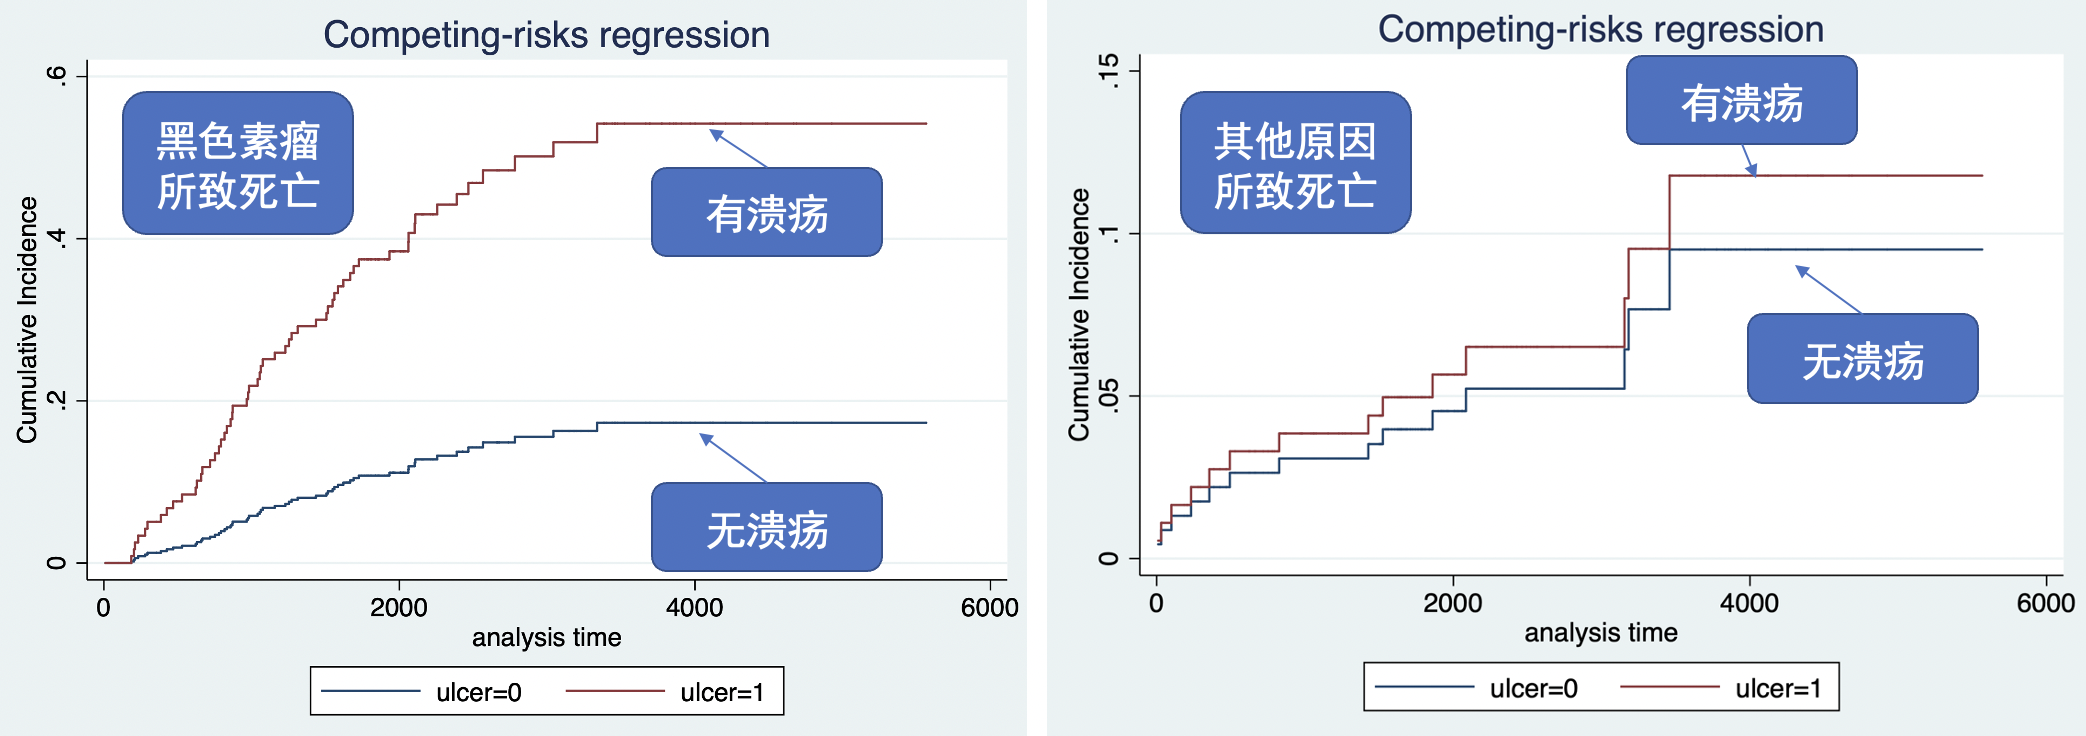
\includegraphics[width=1\linewidth,height=\textheight,keepaspectratio]{chapters/images/ch5-image10.png}

\textbf{代码5.14输出：竞争风险事件的分组累积风险生存曲线}

\subsection{原因别Hazard模型}\label{ux539fux56e0ux522bhazardux6a21ux578b}

竞争结局另外一种比较简单的分析方法，称为原因别Hazard模型。此方法非常易于理解，把不感兴趣的结局事件做人工删失，删失后的新数据中进行Cox回归。

结果与Fine-Gray模型结果一致，有溃疡和没有溃疡的患者因黑色素瘤所致死亡的风险不一致，
p值\textless0.001。

\begin{tcolorbox}[enhanced jigsaw, arc=.35mm, bottomrule=.15mm, breakable, colback=white, colframe=quarto-callout-note-color-frame, left=2mm, leftrule=.75mm, opacityback=0, rightrule=.15mm, toprule=.15mm]

\vspace{-3mm}\textbf{代码5.15}\vspace{3mm}

\begin{Shaded}
\begin{Highlighting}[]
\KeywordTok{generate}\NormalTok{ status\_cause = 2}
\KeywordTok{replace}\NormalTok{ status\_cause = 1 }\KeywordTok{if}\NormalTok{ status == 1}
\KeywordTok{stset}\NormalTok{ time, fail(status\_cause==1)}
\KeywordTok{stcox}\NormalTok{ ulcer}
\end{Highlighting}
\end{Shaded}

\end{tcolorbox}

\begin{tcolorbox}[enhanced jigsaw, arc=.35mm, bottomrule=.15mm, breakable, colback=white, colframe=quarto-callout-note-color-frame, left=2mm, leftrule=.75mm, opacityback=0, rightrule=.15mm, toprule=.15mm]

\vspace{-3mm}\textbf{代码5.15输出}\vspace{3mm}

{\def\LTcaptype{none} % do not increment counter
\begin{longtable}[]{@{}
  >{\raggedright\arraybackslash}p{(\linewidth - 12\tabcolsep) * \real{0.1429}}
  >{\raggedright\arraybackslash}p{(\linewidth - 12\tabcolsep) * \real{0.1429}}
  >{\raggedright\arraybackslash}p{(\linewidth - 12\tabcolsep) * \real{0.1429}}
  >{\raggedright\arraybackslash}p{(\linewidth - 12\tabcolsep) * \real{0.1429}}
  >{\raggedright\arraybackslash}p{(\linewidth - 12\tabcolsep) * \real{0.1429}}
  >{\raggedright\arraybackslash}p{(\linewidth - 12\tabcolsep) * \real{0.1429}}
  >{\raggedright\arraybackslash}p{(\linewidth - 12\tabcolsep) * \real{0.1429}}@{}}
\toprule\noalign{}
\begin{minipage}[b]{\linewidth}\raggedright
Cox regression with no ties
\end{minipage} & \begin{minipage}[b]{\linewidth}\raggedright
\end{minipage} & \begin{minipage}[b]{\linewidth}\raggedright
\end{minipage} & \begin{minipage}[b]{\linewidth}\raggedright
\end{minipage} & \begin{minipage}[b]{\linewidth}\raggedright
\end{minipage} & \begin{minipage}[b]{\linewidth}\raggedright
\end{minipage} & \begin{minipage}[b]{\linewidth}\raggedright
\end{minipage} \\
\midrule\noalign{}
\endhead
\bottomrule\noalign{}
\endlastfoot
No.~of subjects = 205 & Number of obs & = & \textbf{205} & & & \\
No.~of failures = 57 & LR chi2(1) & = & \textbf{28.44} & & & \\
Time at risk = 441,324 & Prob \textgreater{} chi2 & = & \textbf{0.0000}
& & & \\
Log pseudolikelihood = -268.98076 & & & & & & \\
& Haz.ratio & Std. Err. & z & P\textgreater\textbar z\textbar{} &
{[}95\% Conf. Interval{]} & \\
ulcer & \textbf{4.35668} & \textbf{1.286962} & \textbf{4.98} &
\textbf{0.000} & \textbf{2.441805} & \textbf{7.77321} \\
\end{longtable}
}

\end{tcolorbox}

\section{危险比的局限性}\label{ux5371ux9669ux6bd4ux7684ux5c40ux9650ux6027}

估计生存结局的三种主要方法包括危险比（Hazard
Ratio，HR），报告每个治疗组的中位生存期和时间点分析（如1年无进展生存率或总生存率）。HR与其他两种指标在以下方面存在差异。

HR囊括了整个生存曲线中的所有信息，因此总结了整个随访时间内的治疗效果。相比之下，中位生存期仅关注不同干预组生存曲线上的一个点，而作为个体患者疾病控制的生存率指标过于简单。此外，HR提供了不同治疗组之间相对疗效的估计值。最后，可以计算校正和未校正的HR。未校正的HR根据单变量Cox比例风险模型计算，而校正的HR通常使用多变量Cox模型进行，即还包含需要校正的混杂因素，例如年龄、性别、疾病分期和体能状态。与之相对的是，根据生存曲线推导的中位生存期和特定时间点的生存概率往往未进行校正。

然而，HR作为效应指标的局限性。

首先，如果生存曲线严重违背等比例假设，则不适合诠释总体HR，因为HR随时间的变化非常显著。而等比例检验的效能比较低，有时明显违背等比例假设却无法通过等比例检验得出结论。

第二、HR存在内在的选择偏倚，随访中如出现失访，而失访作为删失结局，且如删失与干预措施以及结局事件都相关，那就会出现选择偏倚。

第三、HR是随着时间的变化而产生变化的，随访时间不同产生的HR是不一样的（案例5.1中180天和730天的HR不同），因此计算出的HR只是一个平均值。

第四、HR是相对指标。HR具有统计学意义时，其是否具有临床意义有待评价。为此，临床医生需要结合绝对指标寻找具有一致临床意义的改善，例如特定时间点的生存概率和中位生存期。如对于不同类型的肿瘤，HR
=
0.75可对应于中位生存期50天的改善（有临床意义），亦可对应约10天的改善（可能不具有临床意义）。

最后，将HR推广至研究随访时间后发生的情况应非常谨慎。在缺乏后续信息的情况下，无法确定比例风险假设是否继续成立。不仅如此，后续治疗或姑息治疗也将严重影响患者的生存概率。上述局限性提示，危险比并不总能作为因果效应的恰当度量：由于风险集随时间因死亡而改变，即使在随机试验中，后期的危险比也可能因内在的选择效应而带有偏倚，这一问题被
Hernán（2010）形象地称为``危险比的危害''。因此在解读时应结合生存曲线、限制性平均生存时间与特定时点的绝对风险等指标综合判断。

\section{参考文献}\label{ux53c2ux8003ux6587ux732e-4}

\begin{enumerate}
\def\labelenumi{\arabic{enumi}.}
\item
  Zhang Z, Reinikainen J, Adeleke KA, Pieterse ME, Groothuis-Oudshoorn
  CGM. Time-varying covariates and coefficients in Cox regression
  models. Ann Transl Med. 2018 Apr;6(7):121.
\item
  Gregson J, Sharples L, Stone GW, Burman CF, Öhrn F, Pocock S.
  Nonproportional Hazards for Time-to-Event Outcomes in Clinical Trials:
  JACC Review Topic of~the~Week. J Am Coll Cardiol. 2019 Oct
  22;74(16):2102-2112.
\item
  Cox DR. Regression models and life-tables. Journal of the Royal
  Statistical Society: Series B, 1972, 34(2):187-220.
\item
  Kaplan EL, Meier P. Nonparametric estimation from incomplete
  observations. Journal of the American Statistical Association, 1958,
  53(282):457-481.
\item
  Fine JP, Gray RJ. A proportional hazards model for the subdistribution
  of a competing risk. Journal of the American Statistical Association,
  1999, 94(446):496-509.
\item
  Putter H, Fiocco M, Geskus RB. Tutorial in biostatistics: competing
  risks and multi-state models. Statistics in Medicine, 2007,
  26(11):2389-2430.
\item
  Austin PC, Lee DS, Fine JP. Introduction to the analysis of survival
  data in the presence of competing risks. Circulation, 2016,
  133(6):601-609.
\item
  Royston P, Parmar MK. Restricted mean survival time: an alternative to
  the hazard ratio for the design and analysis of randomized trials with
  a time-to-event outcome. BMC Medical Research Methodology, 2013,
  13:152.
\item
  Dafni U. Landmark analysis at the 25-year landmark point. Circulation:
  Cardiovascular Quality and Outcomes, 2011, 4(3):363-371.
\item
  Hernán MA. The hazards of hazard ratios. Epidemiology, 2010,
  21(1):13-15.
\end{enumerate}

\bookmarksetup{startatroot}

\chapter{荟萃分析基本原理与方法}\label{ux835fux8403ux5206ux6790ux57faux672cux539fux7406ux4e0eux65b9ux6cd5}

Meta分析（Meta-analysis），又称为荟萃分析，是用于比较和综合针对同一科学问题研究结果的统计学方法，常用于系统综述中的定量合并分析。与单个研究相比，通过整合所有相关研究，可更精准地估计医疗干预或卫生政策的效果，并有利于探索各研究证据的一致性及研究间的差异性。而当多个研究结果不一致或都无统计学意义时，采用Meta分析可得到接近真实情况的统计分析结果。但荟萃分析的结论是否有意义取决于纳入研究的质量。系统综述与荟萃分析是循证医学证据的重要基础，其规范的实施流程可参考《Cochrane
干预措施系统评价手册》（Cochrane Handbook）。

荟萃分析的开展可分为八个步骤，每个步骤详述如下。

\section{研究问题的提出}\label{ux7814ux7a76ux95eeux9898ux7684ux63d0ux51fa}

所关注的研究问题是否需要开展荟萃分析来解决？当同一个临床问题有多个已经开展的随机对照研究，但这些研究的结果相互矛盾时，可以开展荟萃分析相互印证，合成一个确定的答案；或者同一个临床问题的随机对照研究样本数量都比较小，未能得出确定性的结论。

如果多个已经开展的随机对照研究已经解答了这个临床问题，再将这些研究的结果汇集在一起是没有意义的，如关于贝伐单抗作为结肠直肠癌辅助治疗的随机对照研究没有显示其能带来益处，三个类似的随机对照研究结果已明确地指出将贝伐单抗添加到结肠直肠癌的辅助化疗中是徒劳的，这时再开展荟萃分析就是多余的了。其次，荟萃分析的一个重要目的是综合来自现有随机对照研究的证据并汇总数据，当荟萃分析的数量超过同一主题的随机对照研究数量时，我们可能得扪心自问初心是否还在。Lancet杂志早在2014年曾提出提高医疗研究的价值并减少浪费，其首要原则就是设定正确的研究重点，以最大化研究潜力，避免多余的研究正是这一原则的体现。重要的是，我们要认识到多余的研究不仅仅是由于错误的方法学，方法正确而与临床无关的研究同样是浪费。荟萃分析作为医学研究中一个重要且强大的工具，可以被正确使用或误用。

\section{撰写荟萃分析方案}\label{ux64b0ux5199ux835fux8403ux5206ux6790ux65b9ux6848}

采用PICOS原则来设计方案，从五个方面考虑：P代表Participants，研究者需考虑研究对象的疾病特征（组织学类型、病情等）和社会人口学特征（种族、年龄、性别等）；I代表Intervention，干预手段，临床研究中主要指治疗方法；C代表Comparison，对照组特征；O代表Outcome，结局指标，应注意定义明确，同时考虑结局指标是二分类、生存变量还是连续型变量，对后期数据提取和统计分析非常重要；S代表Study，研究类型，考虑纳入RCT、队列研究、病例对照研究或者是横断面研究？

研究方案可以在PROSPERO系统（www.crd.york.ac.uk/PROSPERO/）上注册，此系统是由英国国家健康研究所资助创立的国际性前瞻性系统评价注册系统。研究方案的提前注册，一是有助于避免不必要的重复，因为一项荟萃分析的完成通常是耗时耗力的，注册使得研究者能在计划进行系统评价的阶段得以检查是否已经存在类似主题且``正在进行中''的研究，以决定是否有必要继续开展一个新的项目。二是增加研究的透明性，众所周知，系统评价和荟萃分析在循证医学中具有重要的地位，其质量直接关联着许多医疗决策的制定。一个高质量的荟萃分析应该具有透明性、可靠性，并避免偏倚，而实现这些标准的其中一个关键步骤即在研究开始前提前制定方案，对主要研究目的，关键设计和计划分析方法进行界定，这样才能有助于避免偏倚，保证方法的透明性和结果可重复性。

\section{检索研究}\label{ux68c0ux7d22ux7814ux7a76}

检索策略的制定主要从三个方面进行考虑。检索词：常常选择医学主题词（MeSH）结合自由词进行检索，另外检索式的编写，可以参考PICOS的原则。一般检索式中包含所研究的疾病和干预措施。数据库选择：中文通常为万方、维普和CNKI，英文有PubMed、Web
of Science、Embase、Cochrane
Library等；一般至少要检索PubMed，Embase以及COCHRANE三个数据库。研究的发表语言、发表年限有无限制。

文献的检索讲究查全率以及查准率，所以检索还应包括纳入文献的参考文献，相关综述的参考文献，一些会议文献等等。检索到的文献关乎下一步分析，如果检索漏了一两篇关键文献会影响最终结果，如果检索到太多的文献，会增加筛选的工作量。

\section{研究的筛选}\label{ux7814ux7a76ux7684ux7b5bux9009}

一般利用文献管理软件如Endnote，Mendeley等进行研究的筛选；根据纳入排除标准进行，并注意记录排除原因，以及排除的数量。需两名研究人员独立进行，对不一致结果通过讨论解决或找第三人裁决。筛选文献是一个很复杂，很费时的过程，可大致分为粗筛和细筛。粗筛阶段研究者可通过阅读文献标题或摘要决定是否筛除此文献，而细筛阶段则需通读文献的方法与结果部分来决定文献的取舍。

\section{研究质量评估}\label{ux7814ux7a76ux8d28ux91cfux8bc4ux4f30}

通过评估研究质量来判断研究中是否存在偏倚，研究的设计是否符合要求。质量评估依靠量表，随机对照研究可采用Cochrane偏倚风险评价工具，从选择偏倚、实施偏倚、测量偏倚、随访偏倚、报告偏倚和其他偏倚6个方面进行偏倚风险评价（表6.1）。

\textbf{表6.1} \textbf{Cochrane偏倚风险评价工具}

{\def\LTcaptype{none} % do not increment counter
\begin{longtable}[]{@{}
  >{\raggedright\arraybackslash}p{(\linewidth - 10\tabcolsep) * \real{0.0155}}
  >{\raggedright\arraybackslash}p{(\linewidth - 10\tabcolsep) * \real{0.0410}}
  >{\raggedright\arraybackslash}p{(\linewidth - 10\tabcolsep) * \real{0.0805}}
  >{\raggedright\arraybackslash}p{(\linewidth - 10\tabcolsep) * \real{0.3489}}
  >{\raggedright\arraybackslash}p{(\linewidth - 10\tabcolsep) * \real{0.3206}}
  >{\raggedright\arraybackslash}p{(\linewidth - 10\tabcolsep) * \real{0.1879}}@{}}
\toprule\noalign{}
\begin{minipage}[b]{\linewidth}\raggedright
\end{minipage} & \begin{minipage}[b]{\linewidth}\raggedright
\end{minipage} & \begin{minipage}[b]{\linewidth}\raggedright
定义
\end{minipage} & \begin{minipage}[b]{\linewidth}\raggedright
低偏倚风险
\end{minipage} & \begin{minipage}[b]{\linewidth}\raggedright
高偏倚风险
\end{minipage} & \begin{minipage}[b]{\linewidth}\raggedright
不清楚
\end{minipage} \\
\midrule\noalign{}
\endhead
\bottomrule\noalign{}
\endlastfoot
选择偏倚 & 随机序列生成 & 随机序列的方法不恰当导致的选择性偏倚 &
研究者在序列产生过程中描述了随机方法，如：随机数字表、计算机产牛陏机数字、抛硬币法、洗牌或信封、掷骰子抽签法、最小化法等
&
研究者在序列产生过程中描述了非随机的方法，如：根据生日的奇数或偶数产生，由入院日期产生；由住院或就诊号码产生；根据临床医师的判断分配或根据病人意愿分配；基于实验室结果或一系列检查结果分配；根据干预措施的有效性分配
& 序列产生的信息不详，难以判断是``低风险''还是``高风险 \\
& 分配隐蔽 & 由于分配方案隐蔽不完善导致的选择性偏倚 &
受试者或招募受试者的研究人员不能预知分配情況，因为采用以下原因或者等效的方法来隐藏随机分配方案：中心分配（包括电话、网站和药房控制随机）；外形相同且有序的药物容器；不透光的有序的密封信封
&
受试者或招募受试者的研究人员可能会预知分配情況而导致选择性偏倚，如：开放性随机分配表（如随机数字表）；信封缺乏恰当的保护（即信封不是密封的，不是有序的，或不是透明的）；交替或轮流分配；出生日期；病历号；其他明确不能隐藏的方法
&
无充分信息判断``低风险''或``高风险''。通常是隐藏的方法没描述或者没充分的描述而不能给出明确的判断 \\
实施偏倚 & 对受试者、研究人员实施盲法 &
研究中干预措施的分配情況被受试者及研究者知晓导致的偏倚 &
对受试者和研究人员实施盲法，且盲法未被破坏；无盲法或盲法不完善，但结局评价不受到盲法的影响
&
未采用盲法或盲法不完善，结果判断或测量会受到影响；对受试者实施盲法，但盲法可能被破坏
& 无充分信息判断，研究中没有报告 \\
测量偏倚 & 对结局评估者实施盲

法 & 因结局评价者知道干预措施分组情況导致的偏倚 &
对结局评估者实施盲法，且盲法未被破坏；无盲法或盲法不完善，但结局评价不受到盲法的影响
&
未采用盲法或盲法不完善，结果判断或测量会受到影响；对结局评估者实施盲法，但盲法被破坏
& 无充分信息判断，研究中没有报告 \\
随访偏倚 & 结果数据不完整 & 由于不完整的结果数据导致的偏倚 &
无缺失数据；各组间缺失比例和原因相似；缺失数据不影响结果分析（如生存分析中的缺失值）；二分类结局中，缺失数据的比例与观察到的事件相比，不足以严重影响干预效应值；对于连续性变量结局，缺失数据不足以严重影响观察到的效应值；采用恰当的方法处理缺失数据
&
各组间缺失比例不平衡；二分类结局中，缺失数据的比例与观察到的事件相比，足以严重影响干预效应值；对于连续性变量结局，缺失数据足以严重影响观察到的效应值；采用符合方案分析，但违背方案的病例数较多；采用不恰当的方法处理缺失数据
& 信息不全，难以判断数据是否完整；研究末提及数据完整性的问題 \\
报告偏倚 & 选择性报告 & 由于选择性报告结果导致的偏倚 &
有研究方案，且报告了所有预定的结局指标（主要和次要结局）；无研究计划但发表的研究报告中所有期望的结局均已报告
&
未报告所有预先指定的主要结局指标；报告的一个或多个结局指标未采用预先指定的测量或数据分析方法
&
一个或多个结局指标末预先设定（不包括没有预料到的不良反应）；荟萃分析关心的结局指标报告不完善；难以判断是否存在选择性报告结果的风险 \\
其他偏倚 & 其他惼倚 & 此表上述未包含的偏倚 & 无其他偏倚来源 &
如：研究设计有关的潜在偏倚；有造假行为；其他问題 &
没有充分的信息判断是否存在重要偏倚风险 \\
\end{longtable}
}

观察性研究，可以用Newcastle-Ottawa评估量表，从选择、可比性、结果3个方面进行偏倚风险评价（表6.2）。

\textbf{表6.2} \textbf{Newcastle-Ottawa队列研究偏倚风险评价工具}

{\def\LTcaptype{none} % do not increment counter
\begin{longtable}[]{@{}
  >{\raggedright\arraybackslash}p{(\linewidth - 0\tabcolsep) * \real{0.9306}}@{}}
\toprule\noalign{}
\begin{minipage}[b]{\linewidth}\raggedright
\textbf{选择}（此类别下每个编号最多可获得一星）
\end{minipage} \\
\midrule\noalign{}
\endhead
\bottomrule\noalign{}
\endlastfoot
1) 病例队列的代表性

a) 真正代表社区中的平均\_\_\_\_\_\_\_\_\_\_\_\_\_\_\_（描述）*

b) 在某种程度上代表社区中的平均\_\_\_\_\_\_\_\_\_\_\_\_\_\_ *

c) 选定的队里，例如护士、志愿者

d) 没有描述群组的来源 \\
2) 非病例队列的选择

a) 来自与病例人群相同的社区 *

b) 来自不同来源

c) 没有描述非病例组的来源 \\
3) 病例的确定

a) 病例记录（例如手术记录）*

b) 与研究者的结构化面谈 *

c) 书面自我报告

d) 没有描述 \\
4) 证明在研究开始时不存在感兴趣的结果

a) 是 *

b) 没有 \\
\textbf{可比性}（此类别下最多可获得两星） \\
1) 基于设计或分析的队列可比性

a) 对 \_\_\_\_\_\_\_\_\_\_\_\_\_ 的控制（选择最重要的因素）*

b) 对任何其他因素的控制 * \\
\textbf{结果}（此类别下每个编号最多可获得一星） \\
1) 结果评估

a) 独立盲法评价 *

b) 基于病例记录 *

c) 自我报告

d) 没有描述 \\
2) 随访时间是否足够长以产生结局事件

a) 是（为感兴趣的结果选择适当的随访期）*

b) 否 \\
3) 队列随访的充分性

a) 完整的随访 *

b) 失访的受试者不太可能引入偏倚 - 少数受试者失访 *

c) 较多失访，没有描述失访的人

d) 没有声明 \\
\end{longtable}
}

诊断性研究，是比较某种新的诊断方法与金标准的诊断正确率，评估其是否可以用于临床的研究，可以用QUADAS-2量表来进行偏倚评估（表6.3）。

\textbf{表6.3 QUADAS-2诊断性研究偏倚风险评价工具}

{\def\LTcaptype{none} % do not increment counter
\begin{longtable}[]{@{}
  >{\raggedright\arraybackslash}p{(\linewidth - 8\tabcolsep) * \real{0.2000}}
  >{\raggedright\arraybackslash}p{(\linewidth - 8\tabcolsep) * \real{0.2000}}
  >{\raggedright\arraybackslash}p{(\linewidth - 8\tabcolsep) * \real{0.2000}}
  >{\raggedright\arraybackslash}p{(\linewidth - 8\tabcolsep) * \real{0.2000}}
  >{\raggedright\arraybackslash}p{(\linewidth - 8\tabcolsep) * \real{0.2000}}@{}}
\toprule\noalign{}
\begin{minipage}[b]{\linewidth}\raggedright
领域
\end{minipage} & \begin{minipage}[b]{\linewidth}\raggedright
患者选择
\end{minipage} & \begin{minipage}[b]{\linewidth}\raggedright
新诊断方法
\end{minipage} & \begin{minipage}[b]{\linewidth}\raggedright
金标准
\end{minipage} & \begin{minipage}[b]{\linewidth}\raggedright
流程和时间
\end{minipage} \\
\midrule\noalign{}
\endhead
\bottomrule\noalign{}
\endlastfoot
描述 &
描述患者选择的方法；描述纳入的患者（已有的诊断方法、临床表现、新诊断方法的预期用途和设置）
& 描述新诊断方法及其开展与解释方法 & 描述金标准及其开展与解释方法 &
描述研究排除的受试者；描述新诊断方法和金标准之间的时间间隔和受试者接受的任何干预措施 \\
偏倚问题（是、否或不清楚） &
入组受试者是连续的或随机的吗？是否避免了病例对照设计？是否避免了不适当的排除？
&
是否在不了解金标准结果的情况下解释新诊断方法的结果？如果使用了阈值，是否是预先指定的？
&
金标准是否可正确分类受试者？是否在不了解新诊断方法结果的情况下解释了金标准结果？
&
新诊断方法和金标准之间是否有适当的时间间隔？是否所有患者都有金标准？是否所有患者都有相同的金标准？是否所有患者都纳入数据分析？ \\
& 根据上述问题判断是否存在偏倚风险（高、低或不清楚） & & & \\
适用性（高、低或不清楚） & 纳入的患者与荟萃分研究问题不匹配？ &
新诊断方法的开展与解释与荟萃分研究问题不匹配？ &
金标准的开展与解释与荟萃分研究问题不匹配？ & \\
\end{longtable}
}

\section{数据提取}\label{ux6570ux636eux63d0ux53d6}

主要包括文献基本信息（作者、发表时间、刊物等）、研究类型和方法学特征、研究对象特征（社会人口学特征、疾病诊断标准、对照的选择标准等）、干预措施和结局指标测量、效应指标、样本量等。数据同样需要由两名研究人员独立进行，对不一致结果通过讨论解决或找第三人裁决。具体包含以下几个方面：

受试者：年龄、性别、种族、基础疾病、各组多少例受试者、研究所在地区

干预/对照：随机/非随机、剂量、方法、干预期限、合并干预措施

结局：定义、单位、测量方法、随访时间、失访率

\begin{itemize}
\item
  连续变量：平均值，标准差
\item
  分类变量：发生例数，总数
\item
  意向性分析/按方案分析
\item
  次要结局事件
\end{itemize}

\section{数据分析}\label{ux6570ux636eux5206ux6790}

统计分析包括判断异质性、异质性分析、探索结果的稳定性以及发表偏倚。常用的荟萃分析软件有Review
Manager（RevMan），Stata和R。Review
Manager（RevMan）是Cochrane协作网系统评价的标准化专用软件，具备荟萃分析的绝大部分功能、操作简单、结果直观。Stata和R分析功能更为全面和强大，可进行meta回归分析、定量检测发表偏倚、诊断性meta分析等，但需写命令行。

\textbf{案例6.1}

研究问题：比较Beta受体阻滞剂与其他药物，能否降低原发性高血压患者的卒中率与死亡率。文献检索并筛选后共纳入13项随机对照研究，下表即所需要提取的数据，每一行代表一个研究，stroke\_beta代表Beta受体阻断剂组中发生卒中的病例数，stroke\_other代表其它药物组发生卒中的病例数，mort\_beta代表Beta受体阻断剂组中死亡的病例数，mort\_other代表其它药物组死亡的病例数最后两列是Beta受体阻断剂的总纳入病例数和其他药物组总的病例数。

\textbf{案例6.1数据表}

{\def\LTcaptype{none} % do not increment counter
\begin{longtable}[]{@{}
  >{\raggedright\arraybackslash}p{(\linewidth - 14\tabcolsep) * \real{0.1250}}
  >{\raggedright\arraybackslash}p{(\linewidth - 14\tabcolsep) * \real{0.1250}}
  >{\raggedright\arraybackslash}p{(\linewidth - 14\tabcolsep) * \real{0.1250}}
  >{\raggedright\arraybackslash}p{(\linewidth - 14\tabcolsep) * \real{0.1250}}
  >{\raggedright\arraybackslash}p{(\linewidth - 14\tabcolsep) * \real{0.1250}}
  >{\raggedright\arraybackslash}p{(\linewidth - 14\tabcolsep) * \real{0.1250}}
  >{\raggedright\arraybackslash}p{(\linewidth - 14\tabcolsep) * \real{0.1250}}
  >{\raggedright\arraybackslash}p{(\linewidth - 14\tabcolsep) * \real{0.1250}}@{}}
\toprule\noalign{}
\begin{minipage}[b]{\linewidth}\raggedright
Study
\end{minipage} & \begin{minipage}[b]{\linewidth}\raggedright
type
\end{minipage} & \begin{minipage}[b]{\linewidth}\raggedright
stroke\_beta
\end{minipage} & \begin{minipage}[b]{\linewidth}\raggedright
stroke\_other
\end{minipage} & \begin{minipage}[b]{\linewidth}\raggedright
mort\_beta
\end{minipage} & \begin{minipage}[b]{\linewidth}\raggedright
mort\_other
\end{minipage} & \begin{minipage}[b]{\linewidth}\raggedright
n\_beta
\end{minipage} & \begin{minipage}[b]{\linewidth}\raggedright
n\_other
\end{minipage} \\
\midrule\noalign{}
\endhead
\bottomrule\noalign{}
\endlastfoot
1 & Atenolol & 422 & 327 & 820 & 738 & 9618 & 9639 \\
2 & Non-atenolol & / & / & 5 & 4 & 53 & 53 \\
3 & Mixed beta-blockers/diuretics & 118 & 133 & 319 & 337 & 8297 &
8179 \\
4 & Atenolol & 14 & 9 & 17 & 13 & 1157 & 1177 \\
5 & Mixed beta-blockers/diuretics & 32 & 41 & 96 & 101 & 3297 & 3272 \\
6 & Atenolol & 201 & 176 & 893 & 873 & 11309 & 11267 \\
7 & Atenolol & 309 & 232 & 431 & 383 & 4558 & 4605 \\
8 & Atenolol & 56 & 45 & 167 & 134 & 1102 & 1081 \\
9 & Mixed beta-blockers/diuretics & 196 & 159 & 228 & 231 & 5471 &
5410 \\
10 & Mixed beta-blockers/diuretics & 237 & 422 & 369 & 742 & 2213 &
4401 \\
11 & Atenolol & 17 & 21 & 59 & 75 & 358 & 400 \\
12 & Non-atenolol & 6 & 11 & 1 & 7 & 150 & 154 \\
13 & Non-atenolol & 42 & 18 & 120 & 128 & 4403 & 4297 \\
\end{longtable}
}

\subsection{荟萃与森林图}\label{ux835fux8403ux4e0eux68eeux6797ux56fe}

首先计算Beta受体阻滞剂能否降低死亡率。在Stata中，可以利用metan命令来计算合并后的效应，metan后的四个参数，分别是Beta受体阻断剂组的死亡例数，Beta受体阻断剂的总例数，其它药物组的死亡例数和其它药物组的总例数。效应的表示方法可以是风险比（RR），或是比值比（OR）。Stata输出的荟萃分析结果，汇总的比值比为1.034，其95\%置信区间为0.985-1.085，p值为0.174，因此可以得出结论，Beta受体阻断剂与其他药物组相比，并无法显著减低患者的死亡率。

\begin{tcolorbox}[enhanced jigsaw, arc=.35mm, bottomrule=.15mm, breakable, colback=white, colframe=quarto-callout-note-color-frame, left=2mm, leftrule=.75mm, opacityback=0, rightrule=.15mm, toprule=.15mm]

\vspace{-3mm}\textbf{代码6.1}\vspace{3mm}

\begin{Shaded}
\begin{Highlighting}[]
\NormalTok{metan mort\_beta n\_beta mort\_other n\_other, }\KeywordTok{or}
\end{Highlighting}
\end{Shaded}

\end{tcolorbox}

\begin{tcolorbox}[enhanced jigsaw, arc=.35mm, bottomrule=.15mm, breakable, colback=white, colframe=quarto-callout-note-color-frame, left=2mm, leftrule=.75mm, opacityback=0, rightrule=.15mm, toprule=.15mm]

\vspace{-3mm}\textbf{代码6.1输出}\vspace{3mm}

{\def\LTcaptype{none} % do not increment counter
\begin{longtable}[]{@{}lllll@{}}
\toprule\noalign{}
Study & Odds ratio & {[}95\% Conf. Interval{]} & \% Weight & \\
\midrule\noalign{}
\endhead
\bottomrule\noalign{}
\endlastfoot
1 & \textbf{1.114} & \textbf{1.004} & \textbf{1.235} & \textbf{21.02} \\
2 & \textbf{1.250} & \textbf{0.318} & \textbf{4.913} & \textbf{0.11} \\
3 & \textbf{0.933} & \textbf{0.798} & \textbf{1.091} & \textbf{10.06} \\
4 & \textbf{1.330} & \textbf{0.643} & \textbf{2.751} & \textbf{0.39} \\
5 & \textbf{0.943} & \textbf{0.710} & \textbf{1.253} & \textbf{3.03} \\
6 & \textbf{1.019} & \textbf{0.925} & \textbf{1.123} & \textbf{25.00} \\
7 & \textbf{1.137} & \textbf{0.985} & \textbf{1.312} & \textbf{10.79} \\
8 & \textbf{1.223} & \textbf{0.959} & \textbf{1.558} & \textbf{3.66} \\
9 & \textbf{0.976} & \textbf{0.810} & \textbf{1.176} & \textbf{6.87} \\
10 & \textbf{0.989} & \textbf{0.864} & \textbf{1.132} &
\textbf{13.10} \\
11 & \textbf{0.879} & \textbf{0.607} & \textbf{1.272} & \textbf{1.86} \\
12 & \textbf{0.147} & \textbf{0.018} & \textbf{1.207} & \textbf{0.21} \\
13 & \textbf{0.915} & \textbf{0.711} & \textbf{1.178} & \textbf{3.88} \\
Overall, MH & \textbf{1.034} & \textbf{0.986} & \textbf{1.085} &
\textbf{100.00} \\
Test of overall effect = 1: z = 1.370 p = 0.171 & & & & \\
\end{longtable}
}

\end{tcolorbox}

命令执行过程中，系统会自动的做出森林图，其中每一行代表一个研究，最后一行是汇总的比值比。灰色方框的大小代表样本量的多少，此图可以看出研究的样本量越大，其所占权重越大。

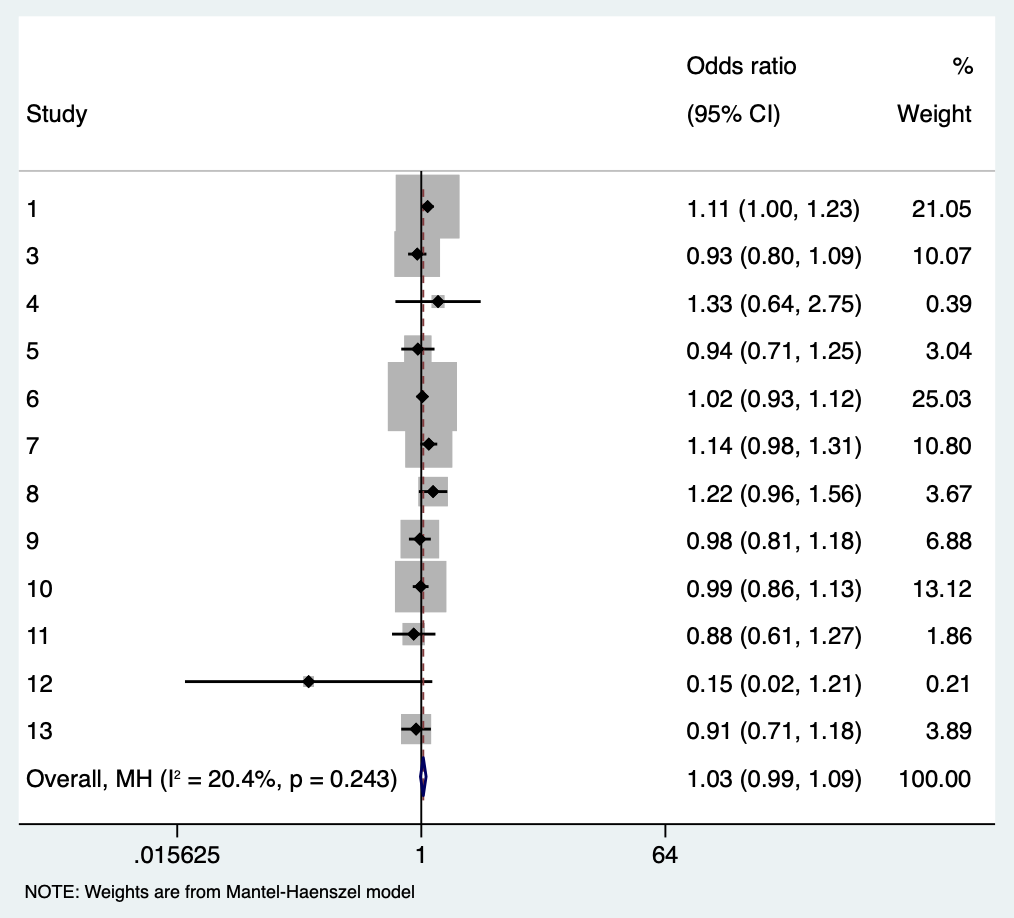
\includegraphics[width=1\linewidth,height=\textheight,keepaspectratio]{chapters/images/ch6-image1.png}

\textbf{代码6.1输出：森林图}

\subsection{异质性分析}\label{ux5f02ux8d28ux6027ux5206ux6790}

荟萃分析中一个非常重要的检验为异质性检验，检验不同的研究间的相似性如何。正式的异质性检验是用卡方分析来进行，但一般而言，利用卡方分析的异质性检验其效能相对较低。I方是另外一种异质性检验的方法。如果I方在25\%以下的话，可以认为异质性较低，如果I方超过50\%，一般认为异质性较高。异质性检验的一个重要作用在于，如果异质性低可以用固定效应模型来进行荟萃分析，但如果异质性较高，则需要采用随机效应模型。本案例中异质性检验的I方是20.4\%，可以认为此研究的异质性较低，采用固定效应模型比较合适。I²
统计量度量的是研究间变异占总变异的比例，其定义与解读可参见 Higgins 与
Thompson（2002）以及 Higgins 等（2003）；需要注意 I²
的取值还受纳入研究数目与样本量的影响，应结合卡方检验与临床判断综合考量。

\begin{tcolorbox}[enhanced jigsaw, arc=.35mm, bottomrule=.15mm, breakable, colback=white, colframe=quarto-callout-note-color-frame, left=2mm, leftrule=.75mm, opacityback=0, rightrule=.15mm, toprule=.15mm]

\vspace{-3mm}\textbf{代码6.1输出：异质性检验}\vspace{3mm}

{\def\LTcaptype{none} % do not increment counter
\begin{longtable}[]{@{}
  >{\raggedright\arraybackslash}p{(\linewidth - 6\tabcolsep) * \real{0.6624}}
  >{\raggedright\arraybackslash}p{(\linewidth - 6\tabcolsep) * \real{0.1720}}
  >{\raggedright\arraybackslash}p{(\linewidth - 6\tabcolsep) * \real{0.0764}}
  >{\raggedright\arraybackslash}p{(\linewidth - 6\tabcolsep) * \real{0.0764}}@{}}
\toprule\noalign{}
\begin{minipage}[b]{\linewidth}\raggedright
Heterogeneity measures, calculated from the data

with Conf. Intervals based on non-central chi² (common-effect)
distribution for Q
\end{minipage} & \begin{minipage}[b]{\linewidth}\raggedright
\end{minipage} & \begin{minipage}[b]{\linewidth}\raggedright
\end{minipage} & \begin{minipage}[b]{\linewidth}\raggedright
\end{minipage} \\
\midrule\noalign{}
\endhead
\bottomrule\noalign{}
\endlastfoot
Measure & Value & df & p-value \\
Mantel-Haenszel Q & \textbf{13.90} & \textbf{12} & \textbf{0.307} \\
& -{[}95\% Conf. Interval{]}- & & \\
H & \textbf{1.076} & \textbf{1.000} & \textbf{1.496} \\
I² (\%) & \textbf{13.7\%} & \textbf{0.0\%} & \textbf{55.3\%} \\
H = relative excess in Mantel-Haenszel Q over its degrees-of-freedom

I² = proportion of total variation in effect estimate due to
between-study heterogeneity (based on Q) & & & \\
\end{longtable}
}

\end{tcolorbox}

使用固定效应模型的前提是每个研究设计比较相似，异质性比较小，因此对于样本量大的那些研究给出的权重就较大。使用随机效应模型是假设不同研究设计是有差别的，研究间的异质性较高。因此荟萃分析给出的每个研究的权重比较均衡，得出的结果也会更加保守，通常认为除非纳入的研究非常相似，更倾向于使用随机效应模型。固定效应模型假设各研究估计的是同一个真实效应，而随机效应模型允许各研究的真实效应服从某一分布，二者的区别与随机效应模型的经典估计方法可参见
DerSimonian 与 Laird（1986）。

然后计算次要结局事件，即Beta受体阻滞剂能否降低患者的卒中发生率。异质性分析
I方达到48.9\%，虽未及50\%，但可认为此研究存在异质性。此时，应该使用随机效应模型计算，metan后指定模型采用随机效应模型（random）。结果提示Beta受体阻滞剂能降低患者的卒中概率，比值比为1.17，95\%置信区间为1.04-1.31，p值为0.010。

\begin{tcolorbox}[enhanced jigsaw, arc=.35mm, bottomrule=.15mm, breakable, colback=white, colframe=quarto-callout-note-color-frame, left=2mm, leftrule=.75mm, opacityback=0, rightrule=.15mm, toprule=.15mm]

\vspace{-3mm}\textbf{代码6.2}\vspace{3mm}

\begin{Shaded}
\begin{Highlighting}[]
\NormalTok{metan stroke\_beta n\_beta stroke\_other n\_other, }\KeywordTok{or}
\end{Highlighting}
\end{Shaded}

\end{tcolorbox}

\begin{tcolorbox}[enhanced jigsaw, arc=.35mm, bottomrule=.15mm, breakable, colback=white, colframe=quarto-callout-note-color-frame, left=2mm, leftrule=.75mm, opacityback=0, rightrule=.15mm, toprule=.15mm]

\vspace{-3mm}\textbf{代码6.2输出：异质性检验}\vspace{3mm}

{\def\LTcaptype{none} % do not increment counter
\begin{longtable}[]{@{}
  >{\raggedright\arraybackslash}p{(\linewidth - 6\tabcolsep) * \real{0.6624}}
  >{\raggedright\arraybackslash}p{(\linewidth - 6\tabcolsep) * \real{0.1720}}
  >{\raggedright\arraybackslash}p{(\linewidth - 6\tabcolsep) * \real{0.0764}}
  >{\raggedright\arraybackslash}p{(\linewidth - 6\tabcolsep) * \real{0.0764}}@{}}
\toprule\noalign{}
\begin{minipage}[b]{\linewidth}\raggedright
Heterogeneity measures, calculated from the data

with Conf. Intervals based on non-central chi² (common-effect)
distribution for Q
\end{minipage} & \begin{minipage}[b]{\linewidth}\raggedright
\end{minipage} & \begin{minipage}[b]{\linewidth}\raggedright
\end{minipage} & \begin{minipage}[b]{\linewidth}\raggedright
\end{minipage} \\
\midrule\noalign{}
\endhead
\bottomrule\noalign{}
\endlastfoot
Measure & Value & df & p-value \\
Mantel-Haenszel Q & \textbf{21.53} & \textbf{11} & \textbf{0.028} \\
& -{[}95\% Conf. Interval{]}- & & \\
H & \textbf{1.399} & \textbf{1.000} & \textbf{1.897} \\
I² (\%) & \textbf{48.9\%} & \textbf{0.0\%} & \textbf{72.2\%} \\
H = relative excess in Mantel-Haenszel Q over its degrees-of-freedom

I² = proportion of total variation in effect estimate due to
between-study heterogeneity (based on Q) & & & \\
\end{longtable}
}

\end{tcolorbox}

\begin{tcolorbox}[enhanced jigsaw, arc=.35mm, bottomrule=.15mm, breakable, colback=white, colframe=quarto-callout-note-color-frame, left=2mm, leftrule=.75mm, opacityback=0, rightrule=.15mm, toprule=.15mm]

\vspace{-3mm}\textbf{代码6.3}\vspace{3mm}

\begin{Shaded}
\begin{Highlighting}[]
\NormalTok{metan stroke\_beta n\_beta stroke\_other n\_other, }\KeywordTok{or}\NormalTok{ random}
\end{Highlighting}
\end{Shaded}

\end{tcolorbox}

\begin{tcolorbox}[enhanced jigsaw, arc=.35mm, bottomrule=.15mm, breakable, colback=white, colframe=quarto-callout-note-color-frame, left=2mm, leftrule=.75mm, opacityback=0, rightrule=.15mm, toprule=.15mm]

\vspace{-3mm}\textbf{代码6.3输出}\vspace{3mm}

{\def\LTcaptype{none} % do not increment counter
\begin{longtable}[]{@{}lllll@{}}
\toprule\noalign{}
Study & Odds ratio & {[}95\% Conf. Interval{]} & \% Weight & \\
\midrule\noalign{}
\endhead
\bottomrule\noalign{}
\endlastfoot
1 & \textbf{1.293} & \textbf{1.116} & \textbf{1.498} & \textbf{15.67} \\
3 & \textbf{0.875} & \textbf{0.681} & \textbf{1.123} & \textbf{10.60} \\
4 & \textbf{1.582} & \textbf{0.682} & \textbf{3.670} & \textbf{1.73} \\
5 & \textbf{0.775} & \textbf{0.487} & \textbf{1.233} & \textbf{4.78} \\
6 & \textbf{1.138} & \textbf{0.928} & \textbf{1.395} & \textbf{12.70} \\
7 & \textbf{1.346} & \textbf{1.129} & \textbf{1.603} & \textbf{14.17} \\
8 & \textbf{1.221} & \textbf{0.817} & \textbf{1.823} & \textbf{5.95} \\
9 & \textbf{1.219} & \textbf{0.986} & \textbf{1.508} & \textbf{12.28} \\
10 & \textbf{1.117} & \textbf{0.945} & \textbf{1.320} &
\textbf{14.60} \\
11 & \textbf{0.904} & \textbf{0.470} & \textbf{1.742} & \textbf{2.71} \\
12 & \textbf{0.560} & \textbf{0.202} & \textbf{1.553} & \textbf{1.21} \\
13 & \textbf{2.277} & \textbf{1.309} & \textbf{3.962} & \textbf{3.61} \\
Overall, DL & \textbf{1.165} & \textbf{1.038} & \textbf{1.308} &
\textbf{100.00} \\
Test of overall effect = 1: z = 2.587 p = 0.010 & & & & \\
\end{longtable}
}

\end{tcolorbox}

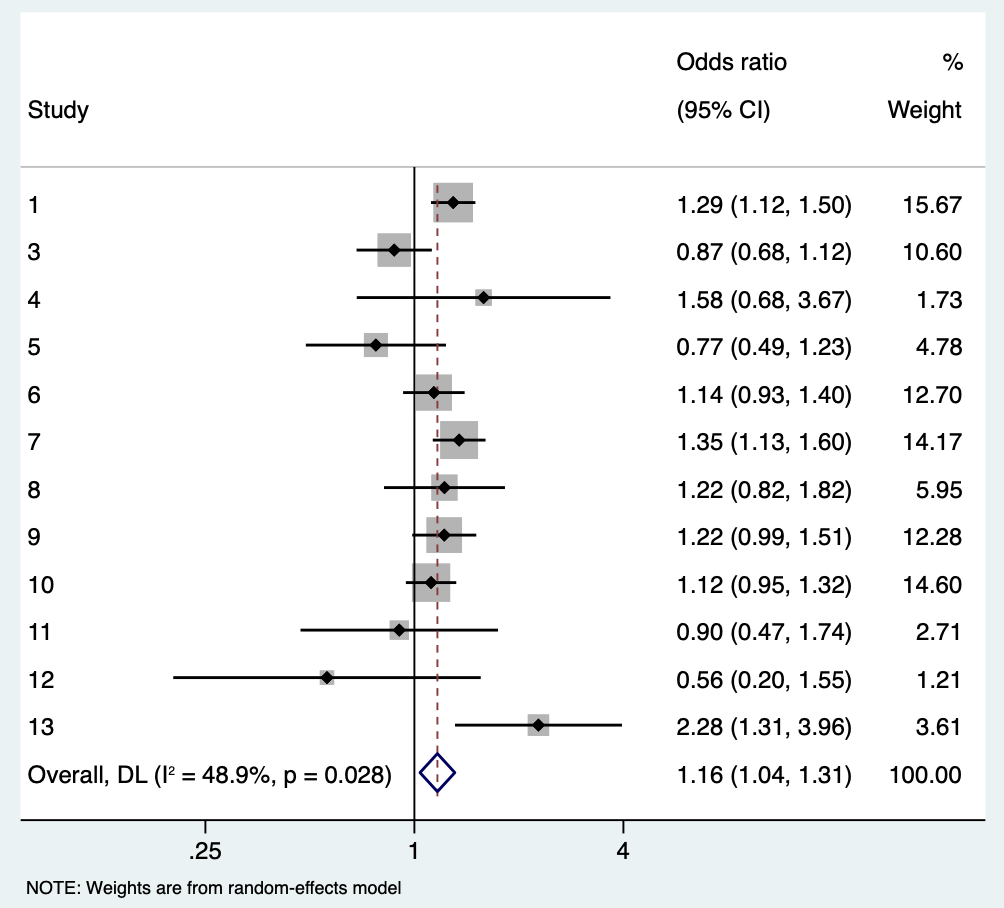
\includegraphics[width=1\linewidth,height=\textheight,keepaspectratio]{chapters/images/ch6-image2.png}

\textbf{代码6.3输出：森林图（随机效应模型）}

虽然荟萃分析提示Beta受体阻滞剂能降低患者的卒中概率，但不同研究中存在异质性，因此需要探索异质性的来源。异质性探索的方法一般是采用分层分析，在各个亚组之间分别进行荟萃分析，metan后指定亚组type。在这个荟萃研究中，纳入研究的Beta受体阻断剂有很多类别，有Atenolol，非Atenolol和混用这三种类别。荟萃分析中可以采用分层分析分别探讨不用药物类别的荟萃效应。森林图分别显示了三种类别的荟萃分析结果，第一个亚组是Atenolol，I方是零，说明这个亚组中的均匀性较好。非Atenolol亚组中只有两个研究，异质性高。第三个亚组是混合组，I方和异质性检验均较高。因此可以得出结论，在Atenolol亚组中，beta受体阻滞剂能够明显降低患者卒中的概率，但在其他两个亚组中的效应可能还需要进一步的研究。

\begin{tcolorbox}[enhanced jigsaw, arc=.35mm, bottomrule=.15mm, breakable, colback=white, colframe=quarto-callout-note-color-frame, left=2mm, leftrule=.75mm, opacityback=0, rightrule=.15mm, toprule=.15mm]

\vspace{-3mm}\textbf{代码6.4}\vspace{3mm}

\begin{Shaded}
\begin{Highlighting}[]
\NormalTok{metan stroke\_beta n\_beta stroke\_other n\_other, }\KeywordTok{or}\NormalTok{ random }\KeywordTok{by}\NormalTok{(}\DecValTok{type}\NormalTok{)}
\end{Highlighting}
\end{Shaded}

\end{tcolorbox}

\begin{tcolorbox}[enhanced jigsaw, arc=.35mm, bottomrule=.15mm, breakable, colback=white, colframe=quarto-callout-note-color-frame, left=2mm, leftrule=.75mm, opacityback=0, rightrule=.15mm, toprule=.15mm]

\vspace{-3mm}\textbf{代码6.4输出}\vspace{3mm}

{\def\LTcaptype{none} % do not increment counter
\begin{longtable}[]{@{}
  >{\raggedright\arraybackslash}p{(\linewidth - 8\tabcolsep) * \real{0.4310}}
  >{\raggedright\arraybackslash}p{(\linewidth - 8\tabcolsep) * \real{0.1121}}
  >{\raggedright\arraybackslash}p{(\linewidth - 8\tabcolsep) * \real{0.2155}}
  >{\raggedright\arraybackslash}p{(\linewidth - 8\tabcolsep) * \real{0.1034}}
  >{\raggedright\arraybackslash}p{(\linewidth - 8\tabcolsep) * \real{0.1121}}@{}}
\toprule\noalign{}
\begin{minipage}[b]{\linewidth}\raggedright
Study
\end{minipage} & \begin{minipage}[b]{\linewidth}\raggedright
Odds ratio
\end{minipage} & \begin{minipage}[b]{\linewidth}\raggedright
{[}95\% Conf. Interval{]}
\end{minipage} & \begin{minipage}[b]{\linewidth}\raggedright
\% Weight
\end{minipage} & \begin{minipage}[b]{\linewidth}\raggedright
\end{minipage} \\
\midrule\noalign{}
\endhead
\bottomrule\noalign{}
\endlastfoot
Atenolol & & & & \\
1 & \textbf{1.293} & \textbf{1.116} & \textbf{1.498} & \textbf{15.67} \\
4 & \textbf{1.582} & \textbf{0.682} & \textbf{3.670} & \textbf{1.73} \\
6 & \textbf{1.138} & \textbf{0.928} & \textbf{1.395} & \textbf{12.70} \\
7 & \textbf{1.346} & \textbf{1.129} & \textbf{1.603} & \textbf{14.17} \\
8 & \textbf{1.221} & \textbf{0.817} & \textbf{1.823} & \textbf{5.95} \\
11 & \textbf{0.904} & \textbf{0.470} & \textbf{1.742} & \textbf{2.71} \\
Subgroup, DL & \textbf{1.263} & \textbf{1.149} & \textbf{1.388} &
\textbf{52.93} \\
Non-atenolol & & & & \\
12 & \textbf{0.560} & \textbf{0.202} & \textbf{1.553} & \textbf{1.21} \\
13 & \textbf{2.277} & \textbf{1.309} & \textbf{3.962} & \textbf{3.61} \\
Subgroup, DL & \textbf{1.209} & \textbf{0.308} & \textbf{4.748} &
\textbf{4.82} \\
Mixed beta-blockers/diuretics & & & & \\
3 & \textbf{0.875} & \textbf{0.681} & \textbf{1.123} & \textbf{10.60} \\
5 & \textbf{0.775} & \textbf{0.487} & \textbf{1.233} & \textbf{4.78} \\
9 & \textbf{1.219} & \textbf{0.986} & \textbf{1.508} & \textbf{12.28} \\
10 & \textbf{1.117} & \textbf{0.945} & \textbf{1.320} &
\textbf{14.60} \\
Subgroup, DL & \textbf{1.035} & \textbf{0.871} & \textbf{1.232} &
\textbf{42.26} \\
Overall, DL & \textbf{1.165} & \textbf{1.038} & \textbf{1.308} &
\textbf{100.00} \\
Tests of subgroup effect size = 1:

Atenolol z = 4.857 p = 0.000

Non-atenolol z = 0.272 p = 0.786

Mixed beta-blockers/diureti z = 0.394 p = 0.694

Overall z = 2.587 p = 0.010 & & & & \\
\end{longtable}
}

\end{tcolorbox}

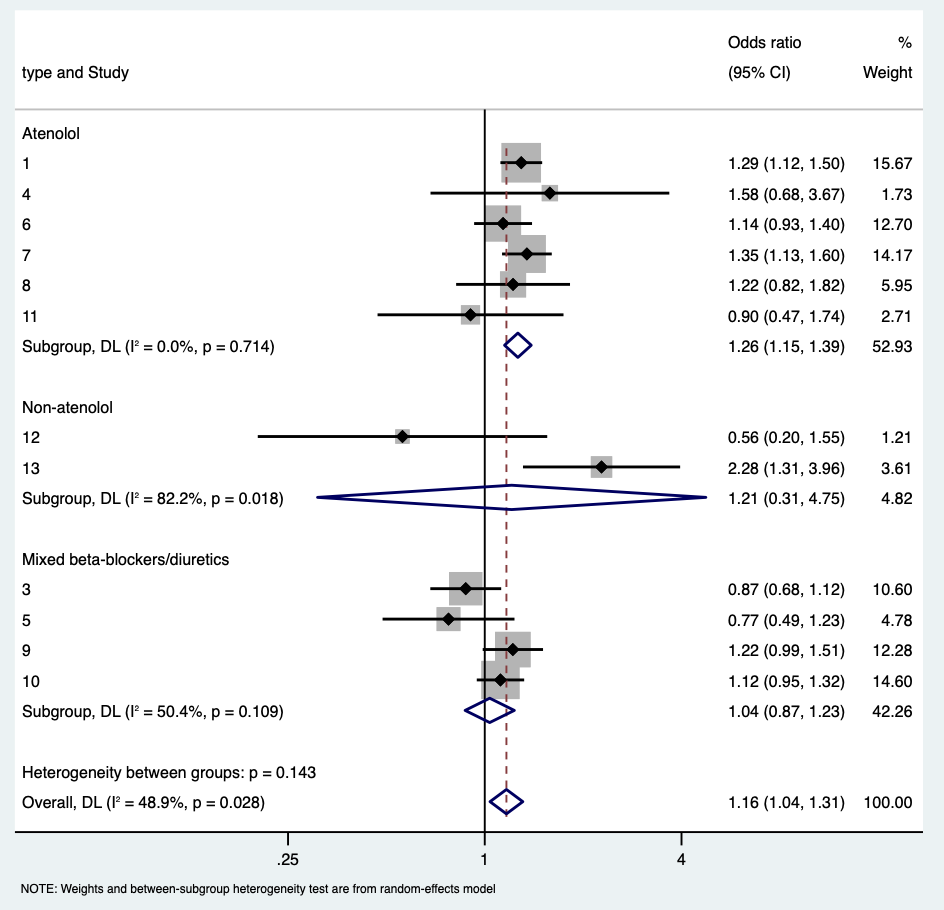
\includegraphics[width=1\linewidth,height=\textheight,keepaspectratio]{chapters/images/ch6-image3.png}

\textbf{代码6.4输出：亚组分析森林图}

\subsection{敏感性分析}\label{ux654fux611fux6027ux5206ux6790}

荟萃分析中的敏感性分析含义是探究单个研究对整体的影响。该分析的步骤是删除纳入的某一项研究，在剩下的研究中进行分析。然后不断重复进行此步骤来观察删除某项研究之后剩下研究中的荟萃分析和全部纳入比较是不是有明显的差别。敏感性分析的结果每一行代表删除该研究后剩余样本中的荟萃结果，可以看到基本上任一单个研究对于整体结果的影响不大。

\begin{tcolorbox}[enhanced jigsaw, arc=.35mm, bottomrule=.15mm, breakable, colback=white, colframe=quarto-callout-note-color-frame, left=2mm, leftrule=.75mm, opacityback=0, rightrule=.15mm, toprule=.15mm]

\vspace{-3mm}\textbf{代码6.5}\vspace{3mm}

\begin{Shaded}
\begin{Highlighting}[]
\NormalTok{metaninf stroke\_beta n\_beta stroke\_other n\_other}
\end{Highlighting}
\end{Shaded}

\end{tcolorbox}

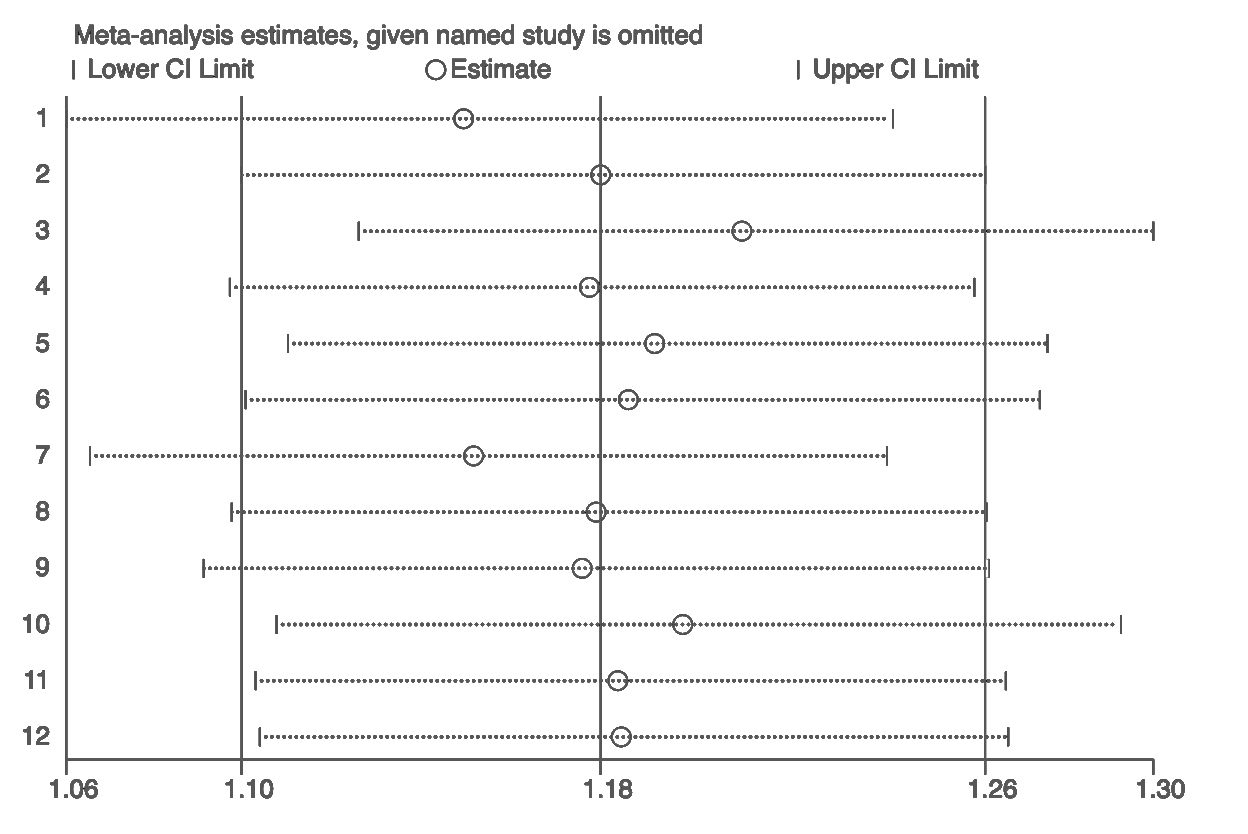
\includegraphics[width=1\linewidth,height=\textheight,keepaspectratio]{chapters/images/ch6-image4.png}

\textbf{代码6.5输出：敏感性分析}

\subsection{发表偏倚}\label{ux53d1ux8868ux504fux501a}

荟萃分析中有一个非常重要的偏倚，称之为发表偏倚。其含义是阳性结果的研究更容易被发表，而阴性结果的研究难以发表。通常使用漏斗图可以明显地检测出这种发表偏倚的存在，漏斗图的X轴表示研究的效应大小，Y轴是效应的标准误，一般而言，样本量大的研究集中在漏斗的顶部，因为这些研究的标准误比较小，而样本量小的研究则分散在漏斗的口部。如果存在发表偏倚，漏斗口部的研究，即样本量较小的研究，会集中在实线的一边。因为样本量小的且具有阳性结果的研究，更容易被发表。本案漏斗图上没有发现明显的发表偏倚。除目测漏斗图是否对称外，还可采用
Egger
等（1997）提出的线性回归法对漏斗图不对称进行正式的统计检验；但当纳入研究数目较少（如少于10项）时，此类检验的效能较低，结果需谨慎解读。

\begin{tcolorbox}[enhanced jigsaw, arc=.35mm, bottomrule=.15mm, breakable, colback=white, colframe=quarto-callout-note-color-frame, left=2mm, leftrule=.75mm, opacityback=0, rightrule=.15mm, toprule=.15mm]

\vspace{-3mm}\textbf{代码6.6}\vspace{3mm}

\begin{Shaded}
\begin{Highlighting}[]
\NormalTok{metafunnel \textbackslash{}\_ES \textbackslash{}\_seES}
\end{Highlighting}
\end{Shaded}

\end{tcolorbox}

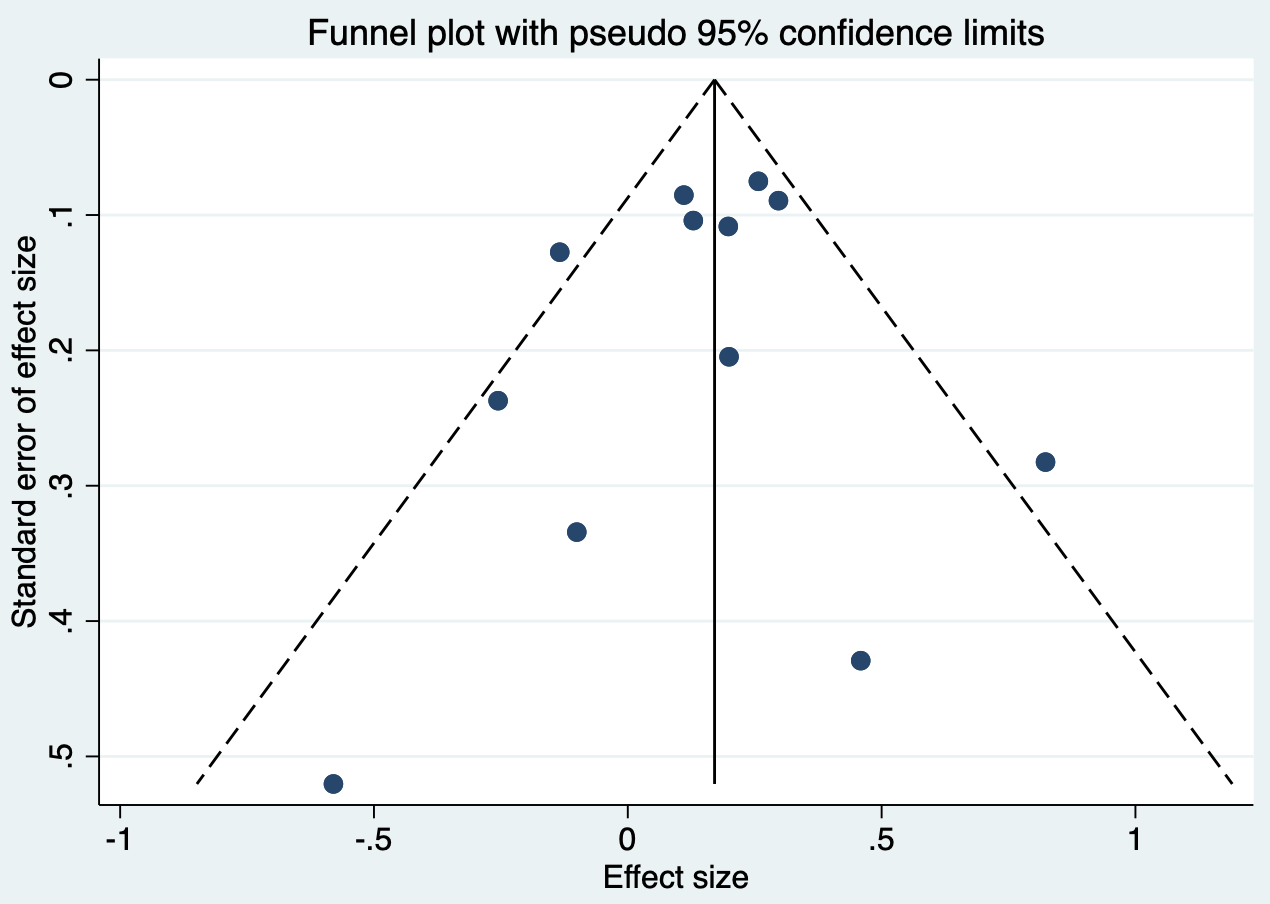
\includegraphics[width=1\linewidth,height=\textheight,keepaspectratio]{chapters/images/ch6-image5.png}

\textbf{代码6.6输出：发表偏倚漏斗图}

\subsection{荟萃回归}\label{ux835fux8403ux56deux5f52}

荟萃回归方法可以探索某一指标与结局效应之间的关系，如研究者想知道是否纳入的病例数越多Beta受体阻滞剂的效应越大。荟萃回归的结果以泡泡图表示，其中每个泡泡代表一个研究，泡泡的大小代表这个研究的样本量，横坐标为纳入例数，纵坐标是效应大小。以效应大小对纳入病例数做回归，可以看到拟合曲线为一条基本水平的直线，因此可以得出结论Beta受体阻滞剂的效应与纳入的病例数无关。荟萃回归用于探索研究层面的协变量对效应大小的影响，其实施与解读（包括生态学谬误与多重检验的风险）可参见
Thompson 与 Higgins（2002）。

\begin{tcolorbox}[enhanced jigsaw, arc=.35mm, bottomrule=.15mm, breakable, colback=white, colframe=quarto-callout-note-color-frame, left=2mm, leftrule=.75mm, opacityback=0, rightrule=.15mm, toprule=.15mm]

\vspace{-3mm}\textbf{代码6.7}\vspace{3mm}

\begin{Shaded}
\begin{Highlighting}[]
\NormalTok{metareg \textbackslash{}\_ES n\_beta, wsse(\textbackslash{}\_seES) }\KeywordTok{graph}
\end{Highlighting}
\end{Shaded}

\end{tcolorbox}

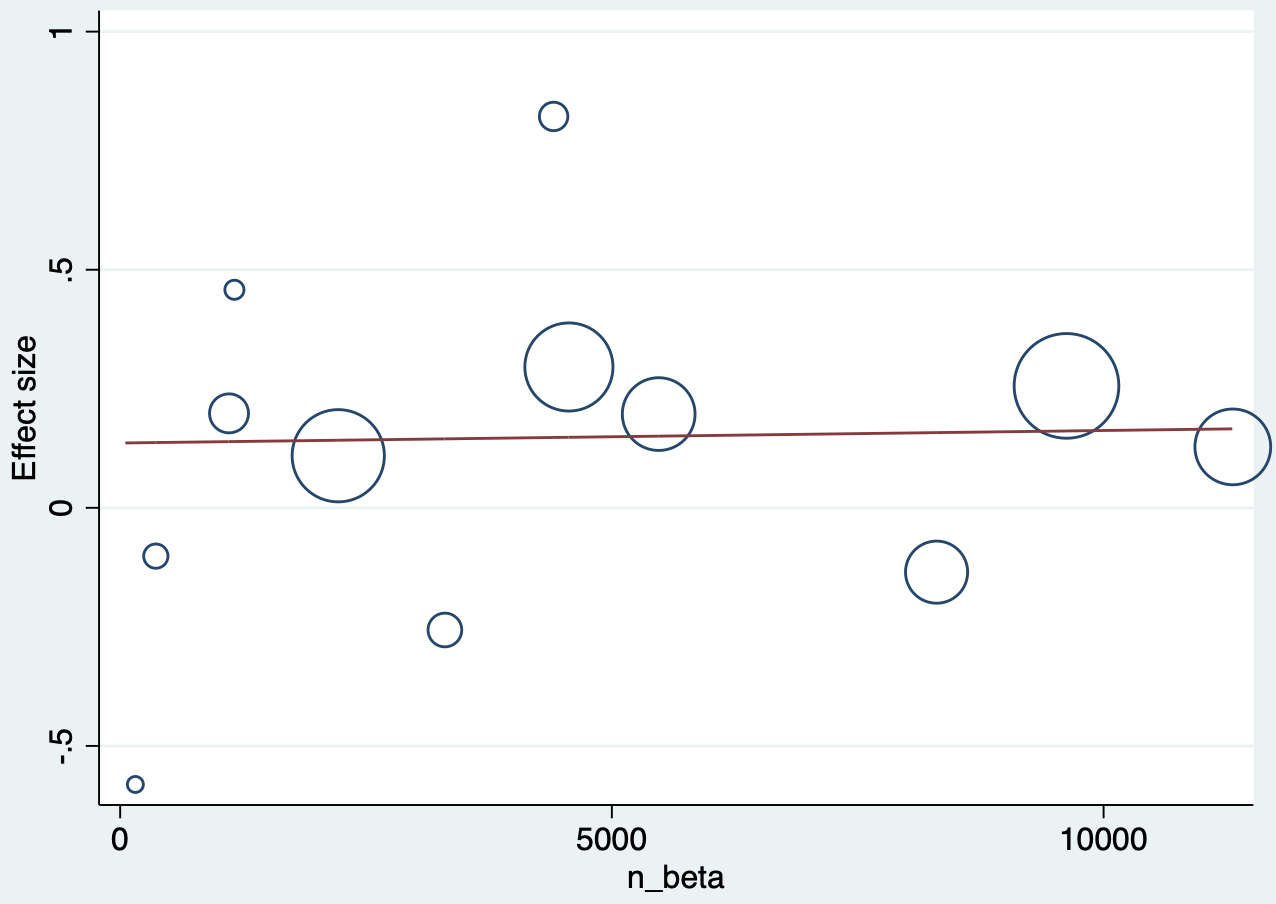
\includegraphics[width=1\linewidth,height=\textheight,keepaspectratio]{chapters/images/ch6-image6.png}

\textbf{代码6.7输出：荟萃回归泡泡图}

\textbf{案例6.2}

案例6.1中结局事件为二变量，即死亡与非死亡，发生卒中与不发生卒中，临床研究中的结局事件亦可为连续变量。帕金森患者采用手术治疗刺激丘脑核团以降低患者的震颤评分，比较刺激手术与空白对照之后的震颤程度的改变。此研究结局事件为干预前后的震颤评分的改变，为连续变量。共纳入五项随机对照研究，每一行一个研究，Stinumber
是刺激手术的纳入例数，Stimean是刺激手术前后震颤评分改变的平均值，Stisd是刺激手术前后评分改变的标准差，Controlnumber
Controlmean和Controlsd分别是空白对照组的纳入例数，震颤评分改变的平均值，震颤评分改变的标准差。

\textbf{案例6.2数据表}

{\def\LTcaptype{none} % do not increment counter
\begin{longtable}[]{@{}
  >{\raggedright\arraybackslash}p{(\linewidth - 14\tabcolsep) * \real{0.0814}}
  >{\raggedright\arraybackslash}p{(\linewidth - 14\tabcolsep) * \real{0.1512}}
  >{\raggedright\arraybackslash}p{(\linewidth - 14\tabcolsep) * \real{0.1279}}
  >{\raggedright\arraybackslash}p{(\linewidth - 14\tabcolsep) * \real{0.1047}}
  >{\raggedright\arraybackslash}p{(\linewidth - 14\tabcolsep) * \real{0.0814}}
  >{\raggedright\arraybackslash}p{(\linewidth - 14\tabcolsep) * \real{0.1744}}
  >{\raggedright\arraybackslash}p{(\linewidth - 14\tabcolsep) * \real{0.1512}}
  >{\raggedright\arraybackslash}p{(\linewidth - 14\tabcolsep) * \real{0.1279}}@{}}
\toprule\noalign{}
\begin{minipage}[b]{\linewidth}\raggedright
Study
\end{minipage} & \begin{minipage}[b]{\linewidth}\raggedright
Sample size
\end{minipage} & \begin{minipage}[b]{\linewidth}\raggedright
Stinumber
\end{minipage} & \begin{minipage}[b]{\linewidth}\raggedright
Stimean
\end{minipage} & \begin{minipage}[b]{\linewidth}\raggedright
Stisd
\end{minipage} & \begin{minipage}[b]{\linewidth}\raggedright
Controlnumber
\end{minipage} & \begin{minipage}[b]{\linewidth}\raggedright
Controlmean
\end{minipage} & \begin{minipage}[b]{\linewidth}\raggedright
Controlsd
\end{minipage} \\
\midrule\noalign{}
\endhead
\bottomrule\noalign{}
\endlastfoot
1 & 251 & 124 & 17.5 & 11.1 & 127 & 1.5 & 11.3 \\
2 & 136 & 101 & 16 & 10.5 & 35 & 3.7 & 13 \\
3 & 366 & 183 & 17.2 & 13.1 & 183 & 0.4 & 13.3 \\
4 & 255 & 134 & 12.3 & 11.2 & 121 & 1.7 & 9.4 \\
5 & 149 & 71 & 19.6 & 15.1 & 78 & 0.4 & 9.5 \\
\end{longtable}
}

结局变量为连续变量时，效应的表示一般选择标准化的平均差（standardized
mean difference,
SMD）。采用标准化平均差的优势是如果纳入的不同的研究结局指标单位不统一或是评分量表不一致，研究与研究之间的结局数值可能差距比较大，采用标准化平均差就可以消除这种问题所带来的影响。

\begin{tcolorbox}[enhanced jigsaw, arc=.35mm, bottomrule=.15mm, breakable, colback=white, colframe=quarto-callout-note-color-frame, left=2mm, leftrule=.75mm, opacityback=0, rightrule=.15mm, toprule=.15mm]

\vspace{-3mm}\textbf{代码6.8}\vspace{3mm}

\begin{Shaded}
\begin{Highlighting}[]
\NormalTok{metan stinumber stimean stisd controlnumber controlmean controlsd}
\end{Highlighting}
\end{Shaded}

\end{tcolorbox}

\begin{tcolorbox}[enhanced jigsaw, arc=.35mm, bottomrule=.15mm, breakable, colback=white, colframe=quarto-callout-note-color-frame, left=2mm, leftrule=.75mm, opacityback=0, rightrule=.15mm, toprule=.15mm]

\vspace{-3mm}\textbf{代码6.8输出}\vspace{3mm}

{\def\LTcaptype{none} % do not increment counter
\begin{longtable}[]{@{}lllll@{}}
\toprule\noalign{}
Study & SMD & {[}95\% Conf. Interval{]} & \% Weight & \\
\midrule\noalign{}
\endhead
\bottomrule\noalign{}
\endlastfoot
1 & \textbf{1.428} & \textbf{1.151} & \textbf{1.706} & \textbf{21.33} \\
2 & \textbf{1.099} & \textbf{0.693} & \textbf{1.506} & \textbf{9.94} \\
3 & \textbf{1.273} & \textbf{1.048} & \textbf{1.497} & \textbf{32.48} \\
4 & \textbf{1.021} & \textbf{0.759} & \textbf{1.282} & \textbf{24.02} \\
5 & \textbf{1.538} & \textbf{1.172} & \textbf{1.904} & \textbf{12.23} \\
Overall, IV & \textbf{1.261} & \textbf{1.132} & \textbf{1.389} &
\textbf{100.00} \\
Test of overall effect = 0: z = 19.284 p = 0.000 & & & & \\
\end{longtable}
}

\end{tcolorbox}

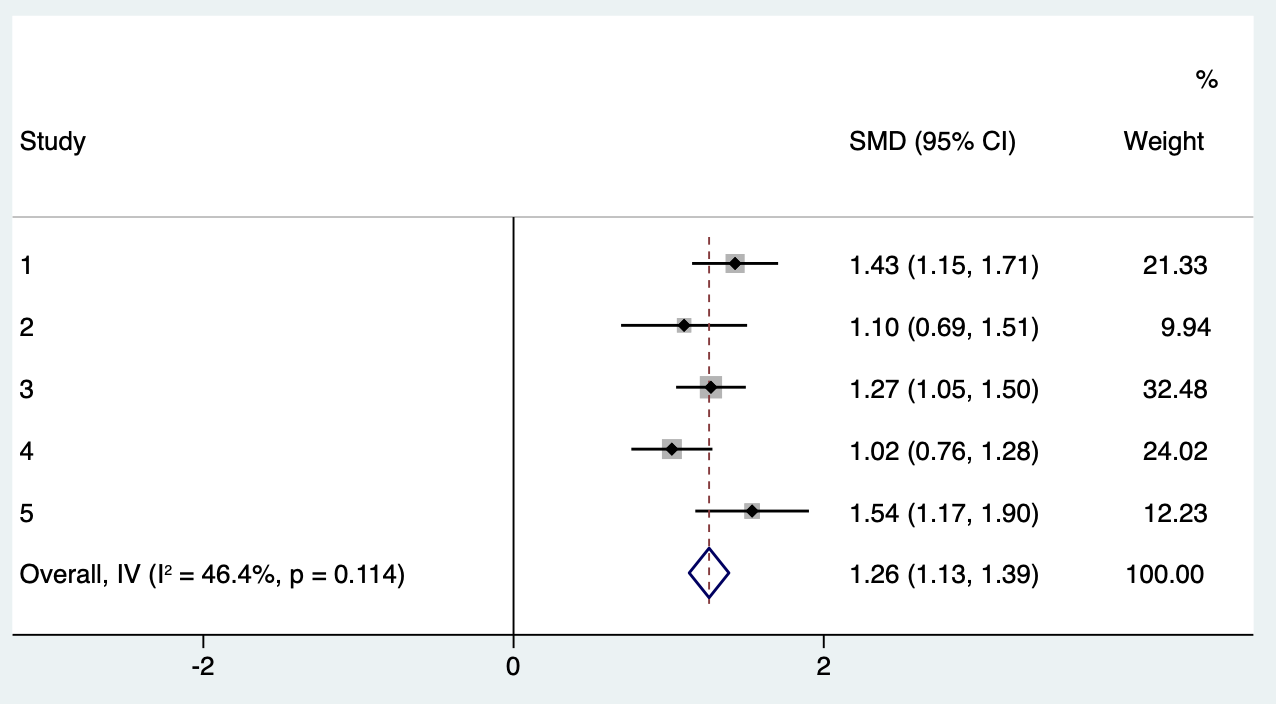
\includegraphics[width=1\linewidth,height=\textheight,keepaspectratio]{chapters/images/ch6-image7.png}

\textbf{代码6.8输出：森林图}

\section{荟萃分析的报告}\label{ux835fux8403ux5206ux6790ux7684ux62a5ux544a}

荟萃分析的报告需要按照一定的规范，PRISMA网站上有荟萃分析的报告清单，具体规范了撰写荟萃分析文章时需要报告哪些内容？其基本内容包括：标题，摘要、背景，方法学，结局讨论等，可具体参考：

http://prisma-statement.org/PRISMAStatement/Checklist.aspx

\textbf{表6.4 PRISMA荟萃分析报告清单}

{\def\LTcaptype{none} % do not increment counter
\begin{longtable}[]{@{}
  >{\raggedright\arraybackslash}p{(\linewidth - 4\tabcolsep) * \real{0.3333}}
  >{\raggedright\arraybackslash}p{(\linewidth - 4\tabcolsep) * \real{0.3333}}
  >{\raggedright\arraybackslash}p{(\linewidth - 4\tabcolsep) * \real{0.3333}}@{}}
\toprule\noalign{}
\begin{minipage}[b]{\linewidth}\raggedright
段落
\end{minipage} & \begin{minipage}[b]{\linewidth}\raggedright
\end{minipage} & \begin{minipage}[b]{\linewidth}\raggedright
条目
\end{minipage} \\
\midrule\noalign{}
\endhead
\bottomrule\noalign{}
\endlastfoot
\textbf{标题部分} & & \\
标题 & 1 & 确定该报告为系统综述 \\
\textbf{摘要部分} & & \\
摘要 & 2 & 参见PRISMA 2020摘要检查表 \\
背景部分 & & \\
理由 & 3 & 描述在现有知识背景下进行回顾的理由。 \\
目的 & 4 & 明确说明该综述的目标或问题。 \\
\textbf{方法部分} & & \\
入组标准 & 5 &
具体说明综述的纳入和排除标准，以及如何对研究进行综合分组。 \\
信息来源 & 6 &
具体说明为确定研究而搜索或查阅的所有数据库、注册、网站、组织、参考文献列表和其他来源。具体说明每个来源最后被搜索的日期。 \\
检索策略 & 7 &
介绍所有数据库、注册和网站的完整检索策略，包括使用的任何过滤器和限制。 \\
筛选过程 & 8 &
具体说明筛选研究是否符合纳入标准的方法，包括有多少名研究者筛选每条记录和检索报告，是否独立工作，以及如果适用的话，该过程中使用的自动化工具的细节。 \\
数据收集过程 & 9 &
具体说明从报告中收集数据的方法，包括有多少名研究者从报告中收集数据，是否独立工作，确认数据的过程，以及如果适用，过程中使用的自动化工具的细节。 \\
数据项目 & 10a &
列出并定义所有结局。具体说明是否寻求每个研究中的所有结局（如测量、时间点、分析方法），是否具有可比性，如果不是，确定收集特殊结果所用的方法。 \\
& 10b &
列出并定义所有其他变量（如受试者和干预特征、资金来源）。说明对任何缺失或不清楚的信息所做的假设。 \\
偏倚评估 & 11 &
具体说明用于评估所纳入研究偏倚风险的方法，包括所使用工具的细节，有多少名研究中评估研究，是否独立工作，如果适用，在此过程中使用的自动化工具的细节。 \\
结局指标 & 12 & 具体说明结局的测量方法（如风险比、平均差异）。 \\
荟萃方法 & 13a &
描述每个研究符合纳入条件的原因（如将研究的干预进行列表并与对照组进行比较） \\
& 13b & 描述准备数据所需的任何方法，如处理缺失或数据转换。 \\
& 13c & 描述是否采用列表或直观显示单个研究结果和综合结果的任何方法。 \\
& 13d &
描述用于荟萃结果的方法，并提供选择这种方法的理由。描述模型、识别统计异质性存在和程度的方法，以及所使用的软件包。 \\
& 13e &
描述任何用于探索研究结果中异质性可能原因的方法（如亚组分析、荟萃回归）。 \\
& 13f & 描述为评估结果稳健性所进行的任何敏感性分析。 \\
报告偏倚 & 14 &
描述任何用于评估研究中因结果缺失而产生偏倚风险的方法（由发表偏倚引起）。 \\
置信评估 & 15 & 描述用于评估结果证据体系置信的任何方法。 \\
\textbf{结果部分} & & \\
研究选择 & 16a &
描述检索和筛选过程的结果，从检索中发现的记录数量到纳入综述的研究数量，最好用流程图来说明。 \\
& 16b &
列举可能符合纳入标准但被排除在外的研究，并解释其被排除的原因。 \\
研究特点 & 17 & 列举每项纳入的研究并介绍其特点。 \\
偏倚评估 & 18 & 对每项纳入的研究进行偏倚风险评估。 \\
每项研究描述 & 19 &
对每项研究提出：每组的汇总统计量（如适用）和效果估计及其精确度（如置信/可信区间），最好使用结构化表格或图表。 \\
荟萃结果 & 20a & 简要总结每项纳入研究的特点和偏倚风险。 \\
& 20b &
介绍所有统计综合的结果。如果进行了荟萃分析，介绍点估计及其精确度（如置信/可信区间）以及统计异质性的测量。如果进行组间比较，说明效果的方向。 \\
& 20c & 对研究结果之间异质性的可能原因以及所有调查结果。 \\
& 20d & 为评估结果的稳健性而进行的所有敏感性分析的结果。 \\
报告偏倚 & 21 &
评估研究中因结果缺失而产生偏倚风险（由发表偏倚引起）。 \\
置信评估 & 22 & 评估结果证据体系的置信。 \\
\textbf{讨论部分} & & \\
讨论 & 23a & 在其他证据的背景下，对结果进行一般性解释。 \\
& 23b & 讨论证据的任何局限性。 \\
& 23c & 讨论所使用综述程序的任何局限性。 \\
& 23d & 讨论结果对实践、政策和未来研究的影响。 \\
\textbf{其他信息} & & \\
注册与方案 & 24a &
提供综述的注册信息，包括注册名称和注册号码，或说明综述没有注册。 \\
& 24b & 说明在哪里可以获得综述方案，或说明没有预先准备方案 \\
& 24c & 描述并解释对预先准备方案中提供信息的任何修正。 \\
资助 & 25 &
说明综述财务或非财务支持的来源，以及资助者或赞助者在审查中的作用。 \\
利益冲突 & 26 & 申报研究者的任何竞争性利益冲突。 \\
数据、代码和其他材料的可得性 & 27 &
报告以下哪些内容是公开的，在哪里可以找到：模板数据收集表；从纳入的研究中提取的数据；用于所有分析的数据；分析代码；任何其他材料。 \\
\end{longtable}
}

\section{参考文献}\label{ux53c2ux8003ux6587ux732e-5}

\begin{enumerate}
\def\labelenumi{\arabic{enumi}.}
\item
  Page MJ, McKenzie JE, Bossuyt PM, Boutron I, Hoffmann TC, Mulrow CD,
  et al.~The PRISMA 2020 statement: an updated guideline for reporting
  systematic reviews. BMJ 2021;372:n71.
\item
  Yang ZR, Sun F, Zhan SY. {[}Risk on bias assessment: (2) Revised
  Cochrane risk of bias tool for individually randomized, parallel group
  trials (RoB2.0){]}. Zhonghua Liu Xing Bing Xue Za Zhi. 2017 Sep
  10;38(9):1285-1291. Chinese.
\item
  Wells G, Shea B, O'Connell D, Peterson J, Welch V, Losos M, Tugwell P.
  The Newcastle-Ottawa Scale (NOS) for assessing the quality of
  nonrandomised studies in meta-analyses.
  2013.~\url{http://www.ohri.ca/programs/clinical_epidemiology/oxford.asp}.
\item
  Whiting PF, Rutjes AW, Westwood ME, Mallett S, Deeks JJ, Reitsma JB,
  Leeflang MM, Sterne JA, Bossuyt PM; QUADAS-2 Group. QUADAS-2: a
  revised tool for the quality assessment of diagnostic accuracy
  studies. Ann Intern Med. 2011 Oct 18;155(8):529-36.
\item
  DerSimonian R, Laird N. Meta-analysis in clinical trials. Controlled
  Clinical Trials, 1986, 7(3):177-188.
\item
  Higgins JPT, Thompson SG. Quantifying heterogeneity in a
  meta-analysis. Statistics in Medicine, 2002, 21(11):1539-1558.
\item
  Higgins JPT, Thompson SG, Deeks JJ, Altman DG. Measuring inconsistency
  in meta-analyses. BMJ, 2003, 327(7414):557-560.
\item
  Egger M, Davey Smith G, Schneider M, Minder C. Bias in meta-analysis
  detected by a simple, graphical test. BMJ, 1997, 315(7109):629-634.
\item
  Thompson SG, Higgins JPT. How should meta-regression analyses be
  undertaken and interpreted? Statistics in Medicine, 2002,
  21(11):1559-1573.
\item
  Higgins JPT, Thomas J, Chandler J, et al.~Cochrane Handbook for
  Systematic Reviews of Interventions. Version 6. Cochrane, 2019.
\end{enumerate}

\bookmarksetup{startatroot}

\chapter{进阶荟萃分析}\label{ux8fdbux9636ux835fux8403ux5206ux6790}

上一章介绍了常规荟萃分析的文献检索、质量评估、数据分析等问题，本章将在此基础上进一步介绍诊断性荟萃分析、网络荟萃分析以及前瞻性荟萃分析的应用。

\section{诊断性研究的荟萃分析}\label{ux8bcaux65adux6027ux7814ux7a76ux7684ux835fux8403ux5206ux6790}

因地区、个体、诊断方法及条件的差异，使得发表的关于同一诊断方法的研究结果存在着不同甚至是矛盾的;
且随着新技术的不断走向临床，选择也愈来愈多。因此，临床上需要综合评价这些研究的结果。在单一诊断试验中，采用某种诊断方法判断为阳性或阴性，然后与金标准阳性和阴性比较，列成四格表的形式，计算相关指标评价该诊断方法的价值。

因而，诊断性研究的荟萃分析主要是为综合评价某种诊断措施对目标疾病的准确率，敏感性、特异性进行评价，报道似然比、诊断优势比等。其中

\textbf{公式7.1　诊断优势比}

\[\text{诊断优势比} = \frac{\text{真阳性}\times\text{真阴性}}{\text{假阳性}\times\text{假阴性}}\]

可作为荟萃分析合并时每个诊断试验权重的依据。

\textbf{案例7.1}

24小时尿游离皮质醇升高是库欣综合征的诊断实验之一，但不同研究报道其准确度不一。从发表文献中搜集研究，提取的数据包括：真阳性，诊断阳性且金标准亦为阳性的例数；假阳性，也就是诊断阳性但金标准为阴性的例数；真阴性，即诊断阴性且金标准为阴性的例数；假阴性，即诊断阴性但金标准为阳性的例数。整理成下表，每一行代表一篇文献，最右边四行分别是TP、TN、FP和FN，分别代表以上这四个数据。

\textbf{案例7.1数据表}

{\def\LTcaptype{none} % do not increment counter
\begin{longtable}[]{@{}lllll@{}}
\toprule\noalign{}
Author & TP & TN & FP & FN \\
\midrule\noalign{}
\endhead
\bottomrule\noalign{}
\endlastfoot
Zukowski 2013 & 3 & 65 & 10 & 0 \\
Yanovski 1998 & 16 & 19 & 1 & 4 \\
Yaneva 2009 & 24 & 69 & 5 & 6 \\
Yaneva 2004 & 63 & 54 & 0 & 0 \\
Viardot 2005 & 12 & 49 & 1 & 0 \\
Valassi 2009 & 52 & 14 & 21 & 3 \\
Tsagarakis 1998 & 57 & 81 & 4 & 3 \\
Tous 2012 & 14 & 40 & 24 & 3 \\
\ldots{} & \ldots{} & \ldots{} & \ldots{} & \ldots{} \\
\end{longtable}
}

Stata中midas命令用于荟萃诊断性研究。

\begin{tcolorbox}[enhanced jigsaw, arc=.35mm, bottomrule=.15mm, breakable, colback=white, colframe=quarto-callout-note-color-frame, left=2mm, leftrule=.75mm, opacityback=0, rightrule=.15mm, toprule=.15mm]

\vspace{-3mm}\textbf{代码7.1}\vspace{3mm}

\begin{Shaded}
\begin{Highlighting}[]
\NormalTok{midas tp fp fn tn, id(author) ms(0.75) bfor(dss)}
\end{Highlighting}
\end{Shaded}

\end{tcolorbox}

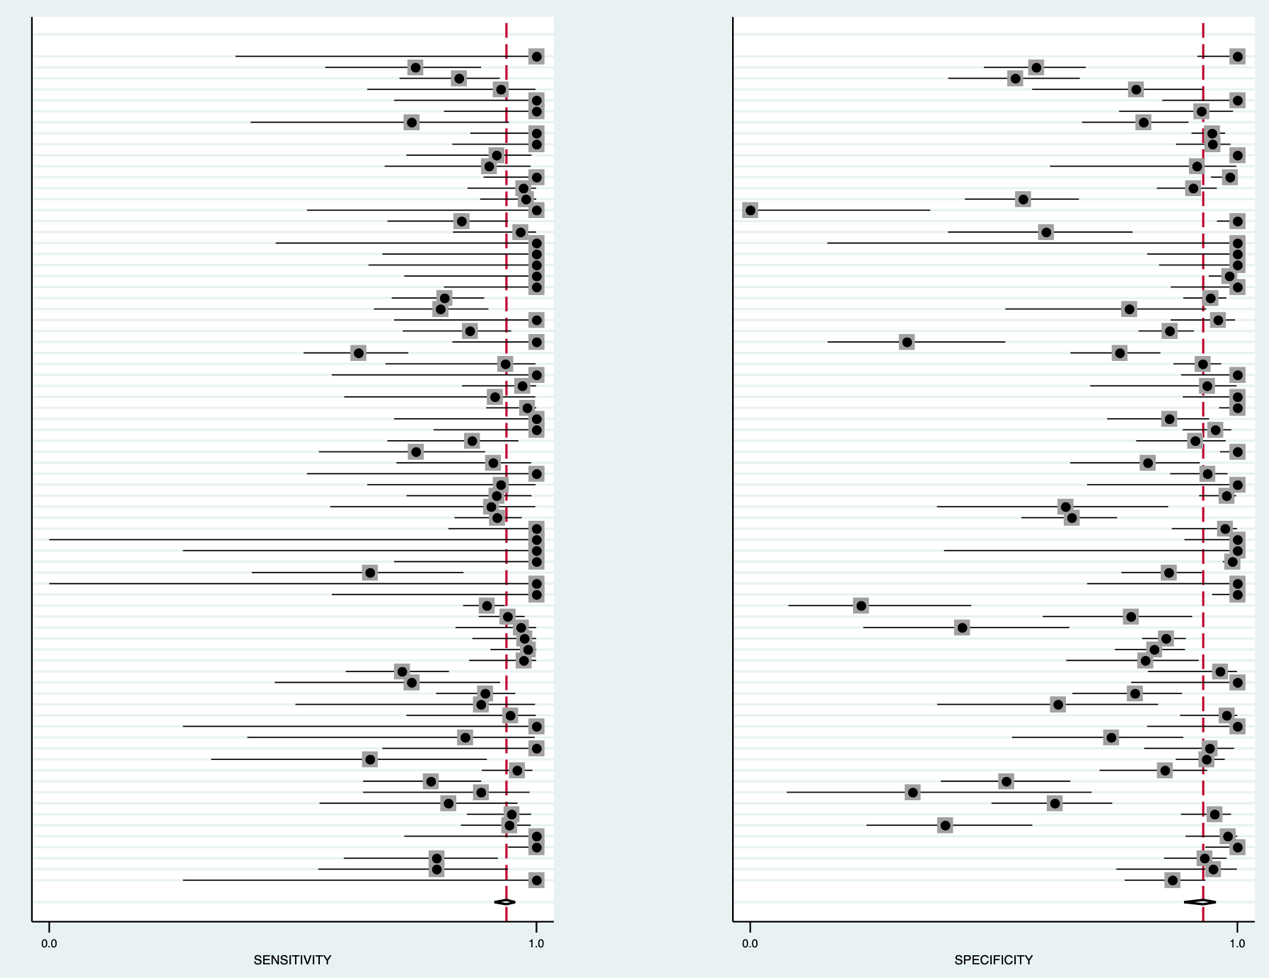
\includegraphics[width=1\linewidth,height=\textheight,keepaspectratio]{chapters/images/ch7-image1.png}

\textbf{代码7.1输出：森林图（左为敏感性，右为特异性）}

敏感性和特异性的森林图，和常规荟萃分析中的森林图是类似的。

\begin{tcolorbox}[enhanced jigsaw, arc=.35mm, bottomrule=.15mm, breakable, colback=white, colframe=quarto-callout-note-color-frame, left=2mm, leftrule=.75mm, opacityback=0, rightrule=.15mm, toprule=.15mm]

\vspace{-3mm}\textbf{代码7.2}\vspace{3mm}

\begin{Shaded}
\begin{Highlighting}[]
\NormalTok{midas tp fp fn tn, es(x) res(}\OtherTok{all}\NormalTok{)}
\end{Highlighting}
\end{Shaded}

\end{tcolorbox}

荟萃所有研究，得出敏感性为94\%、特异性为93\%，诊断优势比为207。有一定的异质性。诊断优势比反映诊断试验的结果与疾病的联系程度。取值
\textgreater1 时，其值越大说明该诊断试验的判别效果较好；取值 \textless1
时，正常人比患者更有可能被诊断试验判为阳性；取值 =1
时，表示该诊断试验无法判别正常人与患者。

\begin{tcolorbox}[enhanced jigsaw, arc=.35mm, bottomrule=.15mm, breakable, colback=white, colframe=quarto-callout-note-color-frame, left=2mm, leftrule=.75mm, opacityback=0, rightrule=.15mm, toprule=.15mm]

\vspace{-3mm}\textbf{代码7.2输出}\vspace{3mm}

{\def\LTcaptype{none} % do not increment counter
\begin{longtable}[]{@{}
  >{\raggedright\arraybackslash}p{(\linewidth - 4\tabcolsep) * \real{0.3333}}
  >{\raggedright\arraybackslash}p{(\linewidth - 4\tabcolsep) * \real{0.3333}}
  >{\raggedright\arraybackslash}p{(\linewidth - 4\tabcolsep) * \real{0.3333}}@{}}
\toprule\noalign{}
\begin{minipage}[b]{\linewidth}\raggedright
ROC Area, AUROC = 0.98 {[}0.96 - 0.99{]}
\end{minipage} & \begin{minipage}[b]{\linewidth}\raggedright
\end{minipage} & \begin{minipage}[b]{\linewidth}\raggedright
\end{minipage} \\
\midrule\noalign{}
\endhead
\bottomrule\noalign{}
\endlastfoot
Heterogeneity (Chi-square): LRT\_Q = 195.006, df =2.00, LRT\_p =0.000 &
& \\
Inconsistency (I-square): LRT\_I2 = 99, 95\% CI = {[} 98- 99{]} & & \\
Parameter & Estimate & 95\% CI \\
Sensitivity & 0.94 & {[}0.92, 0.96{]} \\
Specificity & 0.93 & {[}0.89, 0.96{]} \\
Positive Likelihood Ratio & 13.4 & {[}8.5, 21.2{]} \\
Negative Likelihood Ratio & 0.06 & {[}0.05, 0.09{]} \\
Diagnostic Odds Ratio & 207 & {[}108, 399{]} \\
\end{longtable}
}

\end{tcolorbox}

诊断性研究的荟萃分析中特有的曲线图，即综合ROC曲线（SROC），根据单个诊断试验中的诊断优势比的权重，绘制的集成ROC曲线。SROC曲线上显示每一个研究的灵敏度和特异度。虚线部分是该曲线的95\%置信区间，图上的红点（SROC曲线上最靠近左上角的坐标，灵敏度=特异度）表示对诊断效能的点估计。综合荟萃分析提示24小时尿游离皮质醇对库欣综合征的诊断的敏感性达到了0.94，特异性达到了0.93。诊断准确性荟萃分析推荐采用双变量随机效应模型同时合并敏感性与特异性，并以综合
ROC（SROC）曲线呈现（Reitsma 等，2005）。

\begin{tcolorbox}[enhanced jigsaw, arc=.35mm, bottomrule=.15mm, breakable, colback=white, colframe=quarto-callout-note-color-frame, left=2mm, leftrule=.75mm, opacityback=0, rightrule=.15mm, toprule=.15mm]

\vspace{-3mm}\textbf{代码7.3}\vspace{3mm}

\begin{Shaded}
\begin{Highlighting}[]
\NormalTok{midas tp fp fn tn, plot sroc(both)}
\end{Highlighting}
\end{Shaded}

\end{tcolorbox}

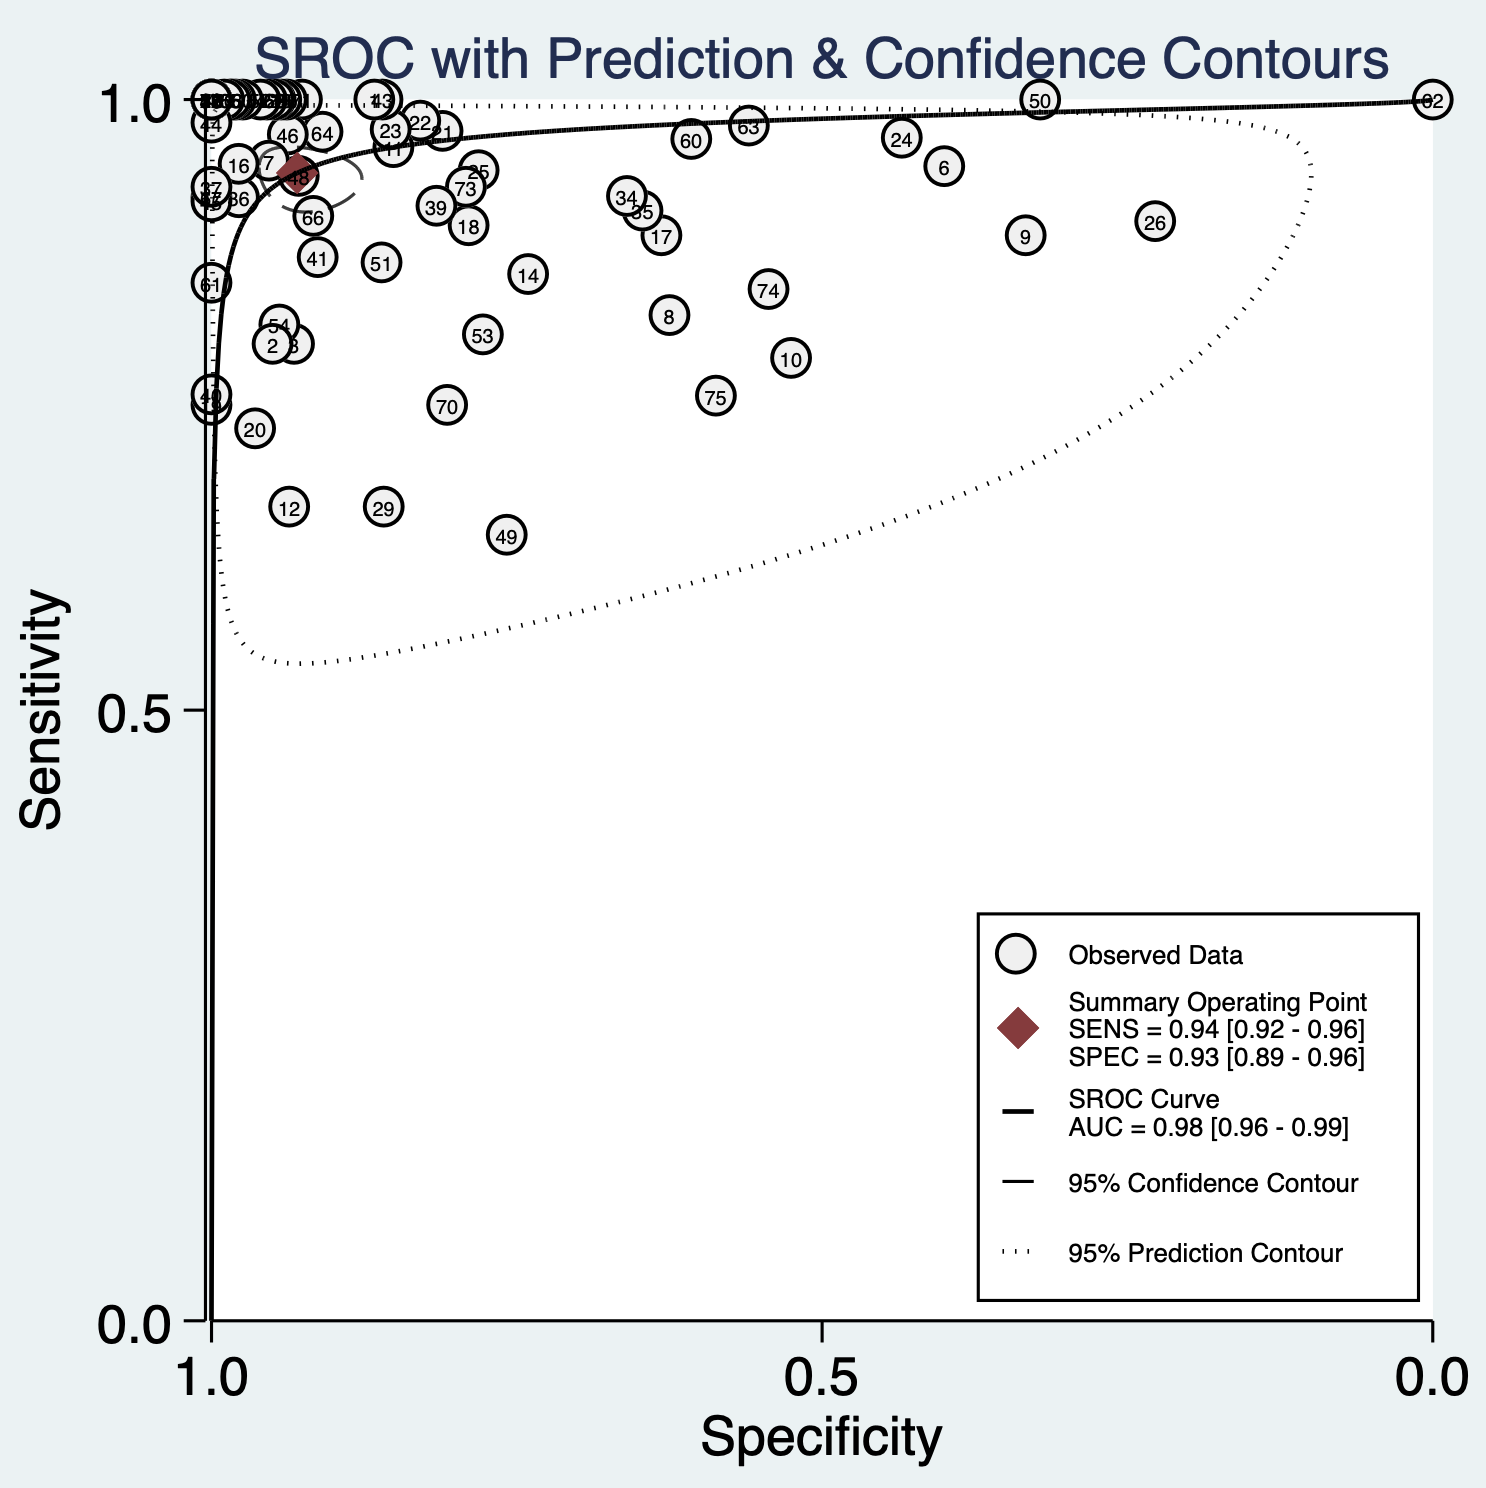
\includegraphics[width=1\linewidth,height=\textheight,keepaspectratio]{chapters/images/ch7-image2.png}

\textbf{代码7.3输出：综合ROC曲线}

\section{网络荟萃分析}\label{ux7f51ux7edcux835fux8403ux5206ux6790}

本书上一章节介绍的荟萃研究关注两种干预措施之间的比较。临床实践中，往往对某一疾病有多种干预，如何比较多种干预措施的疗效？然而，绝大多数临床实验关注的都是两个干预措施之间的比较，如干预A和安慰剂，干预A和干预B。

网络荟萃分析（network meta analysis,
NMA），也被称为多重治疗荟萃分析或混合治疗比较，是一种将多项随机对照研究的证据结合在一起比较治疗方案的方法。在网状荟萃分析当中，需要引入两个概念，直接比较与间接比较（图7.1）。直接比较是指可以直接比较干预A和干预B（即，存在干预A和干预B比较的随机对照研究）。间接比较是存在干预C，有研究探索干预A和干预C的疗效差别，也有研究探索干预B和干预C的疗效差别，但没有研究直接比较干预A和干预B。此时，干预C可以作为纽带，将干预A和干预B连接起来，从而可以去间接的比较干预A和干预B。

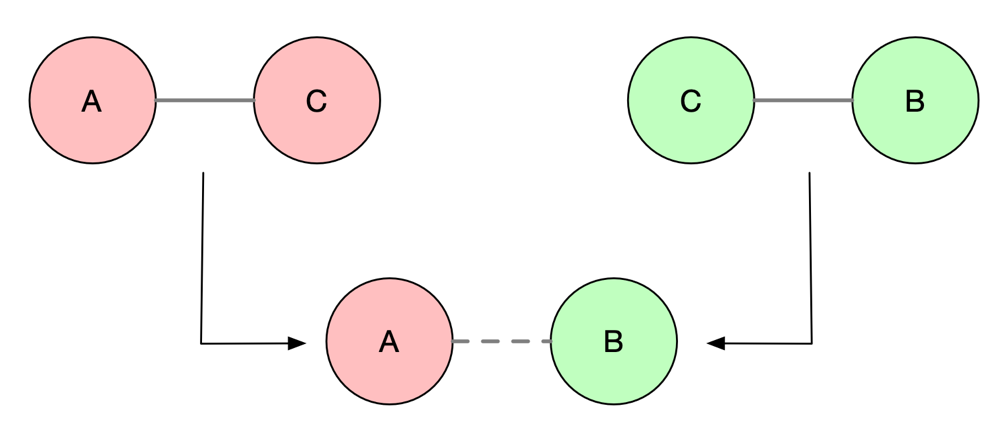
\includegraphics[width=1\linewidth,height=\textheight,keepaspectratio]{chapters/images/ch7-image3.png}

\textbf{图7.1 直接比较和间接比较}

对比传统荟萃分析，网络荟萃分析可以回答更多临床相关问题，可对所有相关的治疗方案进行更全局，更高效地分析。网络荟萃分析可利用所有可获得的证据，获得更精确的结论，对不同治疗方案进行排序，其证据等级相较传统荟萃分析更高。网络荟萃分析的报告应遵循
PRISMA 的网络荟萃分析扩展声明（PRISMA-NMA；Hutton 等，2015）。

网络荟萃分析中一个最重要的统计假设是可传递性（transitivity）。其主要假设研究的人群和干预措施在网络荟萃分析纳入的所有研究中是同质的，或是有理论依据支持干预措施的形式虽然不一样，但实质相同。这种情况下可以认为这些研究中存在可传递性。可传递性是网络荟萃分析有效性的核心前提，应在分析前从临床与方法学上加以论证（Salanti，2012）。

\textbf{案例7.2}

这是一个网络荟萃分析的案例。FDA批准的多发性硬化的干预药物有大概14种之多，在三期临床研究中，60\%是药物直接和安慰剂对比，40\%是药物A和药物B对比。这些研究的结局事件，比较统一，都是治疗后24个月内的复发率。因此选定效应指标为风险比，即两两相比的复发风险比例。网络荟萃分析的数据要求如下表所示。一个研究中的两个组分成两行分别填写入这张表中，并指定研究的名称（studyname）和干预的名称（treatment），填入有效病例数（responders）以及总病例数（sample
size）。

\textbf{案例7.2数据}

{\def\LTcaptype{none} % do not increment counter
\begin{longtable}[]{@{}lllll@{}}
\toprule\noalign{}
studyname & study & responders & sampleSize & treatment \\
\midrule\noalign{}
\endhead
\bottomrule\noalign{}
\endlastfoot
IFNB MS Group & 1 & 18 & 123 & placebo \\
IFNB MS Group & 1 & 59 & 249 & betaseron \\
BRAVO & 2 & 227 & 450 & placebo \\
BRAVO & 2 & 264 & 447 & avonex \\
BRAVO & 2 & 233 & 434 & laquin \\
MSCRG & 3 & 23 & 143 & placebo \\
MSCRG & 3 & 32 & 158 & avonex \\
PRISMS & 4 & 28 & 187 & placebo \\
PRISMS & 4 & 105 & 373 & rebif \\
\ldots{} & & \ldots{} & \ldots{} & \ldots{} \\
\end{longtable}
}

\subsection{网络设置}\label{ux7f51ux7edcux8bbeux7f6e}

利用这张表可以进行网络荟萃分析的数据分析，Stata中首先需要利用network
setup进行网络设置，指定有效病例数与总样本量。然后绘制网络图，以显示哪些治疗与其他哪些治疗直接比较，以及每个治疗和每个治疗比较大约有多少信息可用（通过权重和着色显示证据数量和质量）。图中蓝色圆圈代表干预的方法，其大小代表该干预措施的病例数。黑色连线代表两两干预之间的直接比较，其粗细代表两两对比研究的数量。毋庸置疑，安慰剂组的受试者数量最多，Copaxone和安慰剂组头对头比较的研究数量最多。若圆圈之间无连线，代表没有直接对比这两者的研究。

\begin{tcolorbox}[enhanced jigsaw, arc=.35mm, bottomrule=.15mm, breakable, colback=white, colframe=quarto-callout-note-color-frame, left=2mm, leftrule=.75mm, opacityback=0, rightrule=.15mm, toprule=.15mm]

\vspace{-3mm}\textbf{代码7.4}\vspace{3mm}

\begin{Shaded}
\begin{Highlighting}[]
\NormalTok{network setup responders samplesize, studyvar(study) trtvar(treatment)}
\NormalTok{network map}
\end{Highlighting}
\end{Shaded}

\end{tcolorbox}

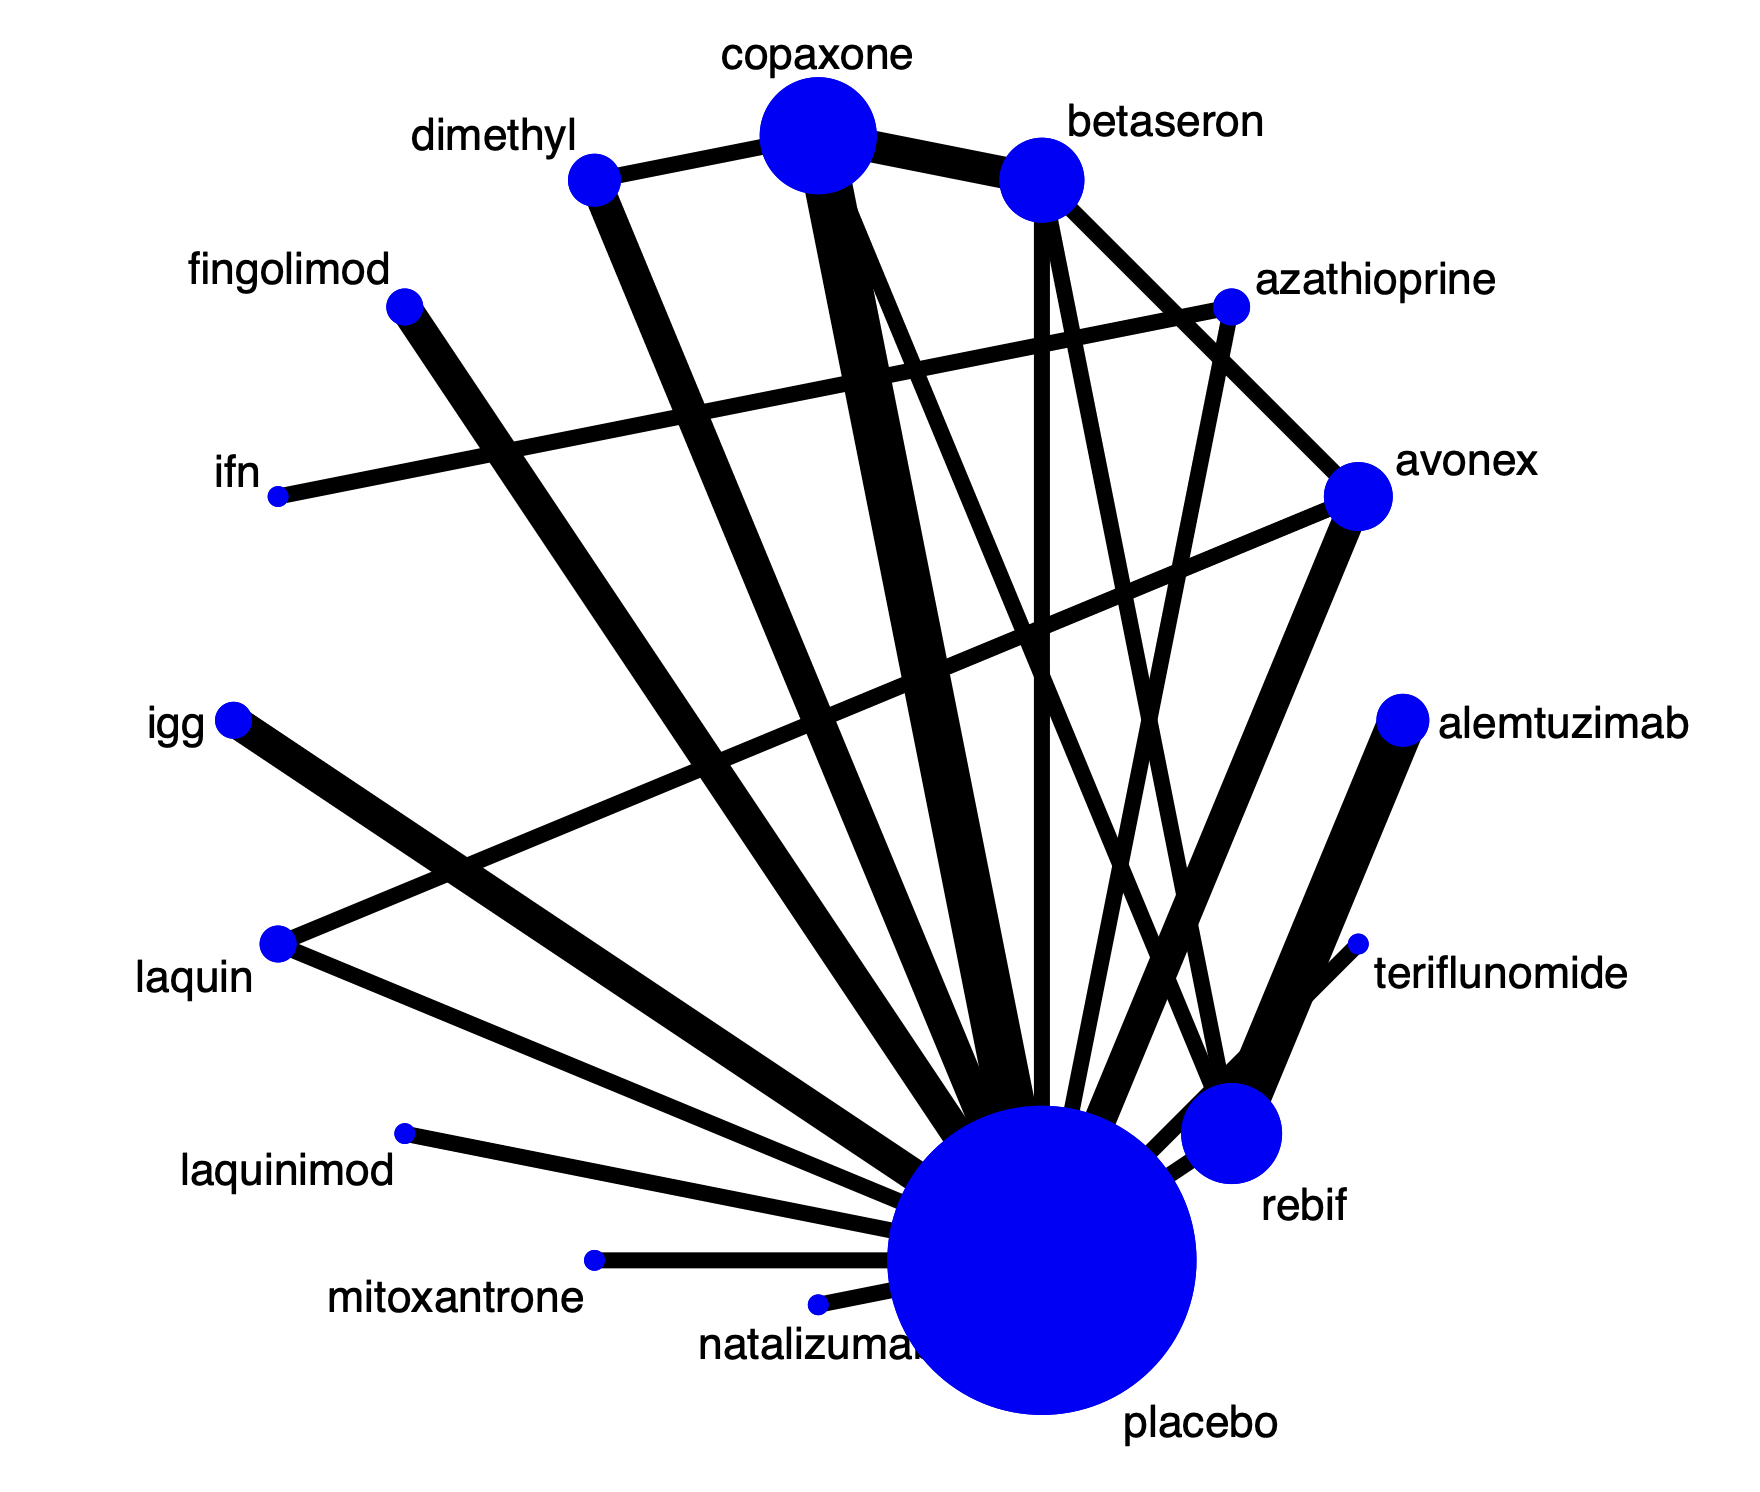
\includegraphics[width=1\linewidth,height=\textheight,keepaspectratio]{chapters/images/ch7-image4.png}

\textbf{代码7.4输出：网络图}

\subsection{干预排序}\label{ux5e72ux9884ux6392ux5e8f}

网络荟萃分析中的累积排序曲线（surface under the cumulative ranking
curve,
SUCRA），其曲线下的面积被用来对每种治疗方法的有效性进行排序，并确定最佳治疗。每一种干预措施都会得出一个累积排序曲线，横坐标表示排序，纵坐标代表这个排序的概率。通常，某条曲线的最高点，代表该治疗方式概率最大的排名名次。图中，mitoxantrone这个干预在排序第一的概率为0.6左右，而placebo在排序第16的概率为0.6左右。

\begin{tcolorbox}[enhanced jigsaw, arc=.35mm, bottomrule=.15mm, breakable, colback=white, colframe=quarto-callout-note-color-frame, left=2mm, leftrule=.75mm, opacityback=0, rightrule=.15mm, toprule=.15mm]

\vspace{-3mm}\textbf{代码7.5}\vspace{3mm}

\begin{Shaded}
\begin{Highlighting}[]
\NormalTok{network meta consistency}
\NormalTok{network }\FunctionTok{rank} \FunctionTok{max}\NormalTok{, }\OtherTok{all} \BaseNTok{zero} \KeywordTok{gen}\NormalTok{(}\KeywordTok{prob}\NormalTok{)}
\NormalTok{sucra }\KeywordTok{prob}\NormalTok{\textbackslash{}*, rankograms labels (alemtuzimab avonex azathioprine betaseron copaxone dimethyl fingolimod ifn igg laquin laquinimod mitoxantrone natalizumab placebo rebif teriflunomide)}
\end{Highlighting}
\end{Shaded}

\end{tcolorbox}


\includegraphics[width=1\linewidth,height=\textheight,keepaspectratio]{chapters/images/ch7-image5.png}

\textbf{代码7.5输出：累积排序曲线}

此外，累积排序曲线下面积也可以通过数值的方式显示。下表展示了各种干预措施的曲线下面积，排序为第一的概率以及平均排序，其中mitoxantrone排序为第一的概率是57.2\%，alemtuzimab排序为第一的概率是33.6\%。因此我们可以得出结论，mitoxantrone在所有干预措施中排序是最高的，即为最佳的干预药物。需要强调的是，SUCRA
仅反映排序概率，并不直接说明治疗之间的差异是否具有临床意义，其计算与解读可参见
Salanti 等（2011）。

\begin{tcolorbox}[enhanced jigsaw, arc=.35mm, bottomrule=.15mm, breakable, colback=white, colframe=quarto-callout-note-color-frame, left=2mm, leftrule=.75mm, opacityback=0, rightrule=.15mm, toprule=.15mm]

\vspace{-3mm}\textbf{代码7.5输出}\vspace{3mm}

{\def\LTcaptype{none} % do not increment counter
\begin{longtable}[]{@{}llll@{}}
\toprule\noalign{}
Treatment & SUCRA & PrBest & MeanRank \\
\midrule\noalign{}
\endhead
\bottomrule\noalign{}
\endlastfoot
alemtuzimab & \textbf{94.3} & \textbf{33.6} & \textbf{1.9} \\
avonex & \textbf{20.8} & \textbf{0.0} & \textbf{12.9} \\
azathioprine & \textbf{69.0} & \textbf{6.5} & \textbf{5.6} \\
betaseron & \textbf{51.7} & \textbf{0.0} & \textbf{8.2} \\
copaxone & \textbf{52.9} & \textbf{0.0} & \textbf{8.1} \\
dimethyl & \textbf{27.7} & \textbf{0.0} & \textbf{11.8} \\
fingolimod & \textbf{60.3} & \textbf{0.0} & \textbf{6.9} \\
ifn & \textbf{50.5} & \textbf{2.0} & \textbf{8.4} \\
igg & \textbf{65.2} & \textbf{0.6} & \textbf{6.2} \\
laquin & \textbf{9.0} & \textbf{0.0} & \textbf{14.7} \\
laquinimod & \textbf{48.8} & \textbf{0.0} & \textbf{8.7} \\
mitoxantrone & \textbf{92.4} & \textbf{57.2} & \textbf{2.1} \\
natalizumab & \textbf{81.6} & \textbf{0.1} & \textbf{3.8} \\
placebo & \textbf{3.5} & \textbf{0.0} & \textbf{15.5} \\
rebif & \textbf{49.0} & \textbf{0.0} & \textbf{8.7} \\
teriflunomide & \textbf{23.3} & \textbf{0.0} & \textbf{12.5} \\
\end{longtable}
}

\end{tcolorbox}

网络荟萃分析中的联赛表，就像足球联赛中，显示两两对决的比分。这张联赛表显示了两种药物之间的两两比较，以风险比展示。中间蓝色方格，代表不同的治疗方案，具体数字，代表比值比以及95\%置信区间，是横排与竖排之间的比较结果。但由于不存在足球联赛中的主客场制，右上部分因与左下部分是重叠的，故予删除。

\begin{tcolorbox}[enhanced jigsaw, arc=.35mm, bottomrule=.15mm, breakable, colback=white, colframe=quarto-callout-note-color-frame, left=2mm, leftrule=.75mm, opacityback=0, rightrule=.15mm, toprule=.15mm]

\vspace{-3mm}\textbf{代码7.6}\vspace{3mm}

\begin{Shaded}
\begin{Highlighting}[]
\NormalTok{netleague, }\KeywordTok{eform}
\end{Highlighting}
\end{Shaded}

\end{tcolorbox}

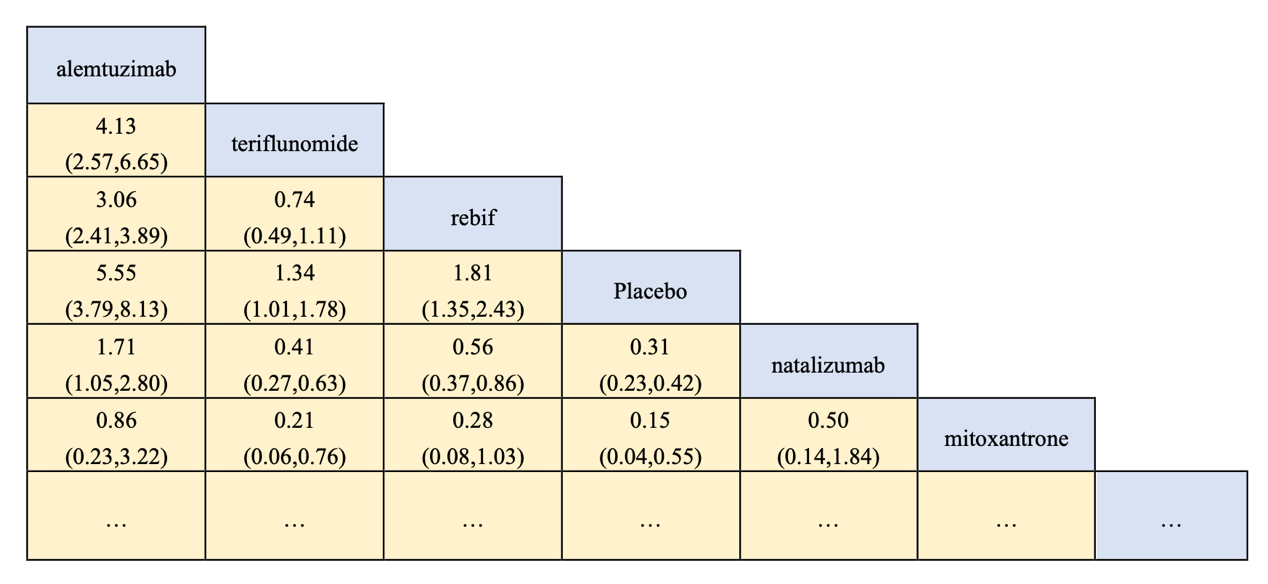
\includegraphics[width=1\linewidth,height=\textheight,keepaspectratio]{chapters/images/ch7-image6.png}

\textbf{代码7.6输出：联赛图}

\subsection{网络一致性}\label{ux7f51ux7edcux4e00ux81f4ux6027}

网络荟萃分析的一个关键问题是网络的一致性。对于某两种干预措施，可能既存在直接证据又可通过间接比较计算间接证据。我们需要检验直接证据和间接证据是否一致，或者如果有多个间接证据来源，则它们是否彼此一致。一致性检验的森林图中p值为0.852，因此可以认为，研究纳入的随机对照研究的一致性较好。森林图中也可以看到间接的两两对比（绿色方块）和直接的两两对比（蓝色方块）基本上得出的结论是一致的。如果检验结果为不一致，可以使用不一致性的统计模型来进行荟萃。

\begin{tcolorbox}[enhanced jigsaw, arc=.35mm, bottomrule=.15mm, breakable, colback=white, colframe=quarto-callout-note-color-frame, left=2mm, leftrule=.75mm, opacityback=0, rightrule=.15mm, toprule=.15mm]

\vspace{-3mm}\textbf{代码7.7}\vspace{3mm}

\begin{Shaded}
\begin{Highlighting}[]
\NormalTok{network meta inconsistency}
\NormalTok{network forest}
\end{Highlighting}
\end{Shaded}

\end{tcolorbox}

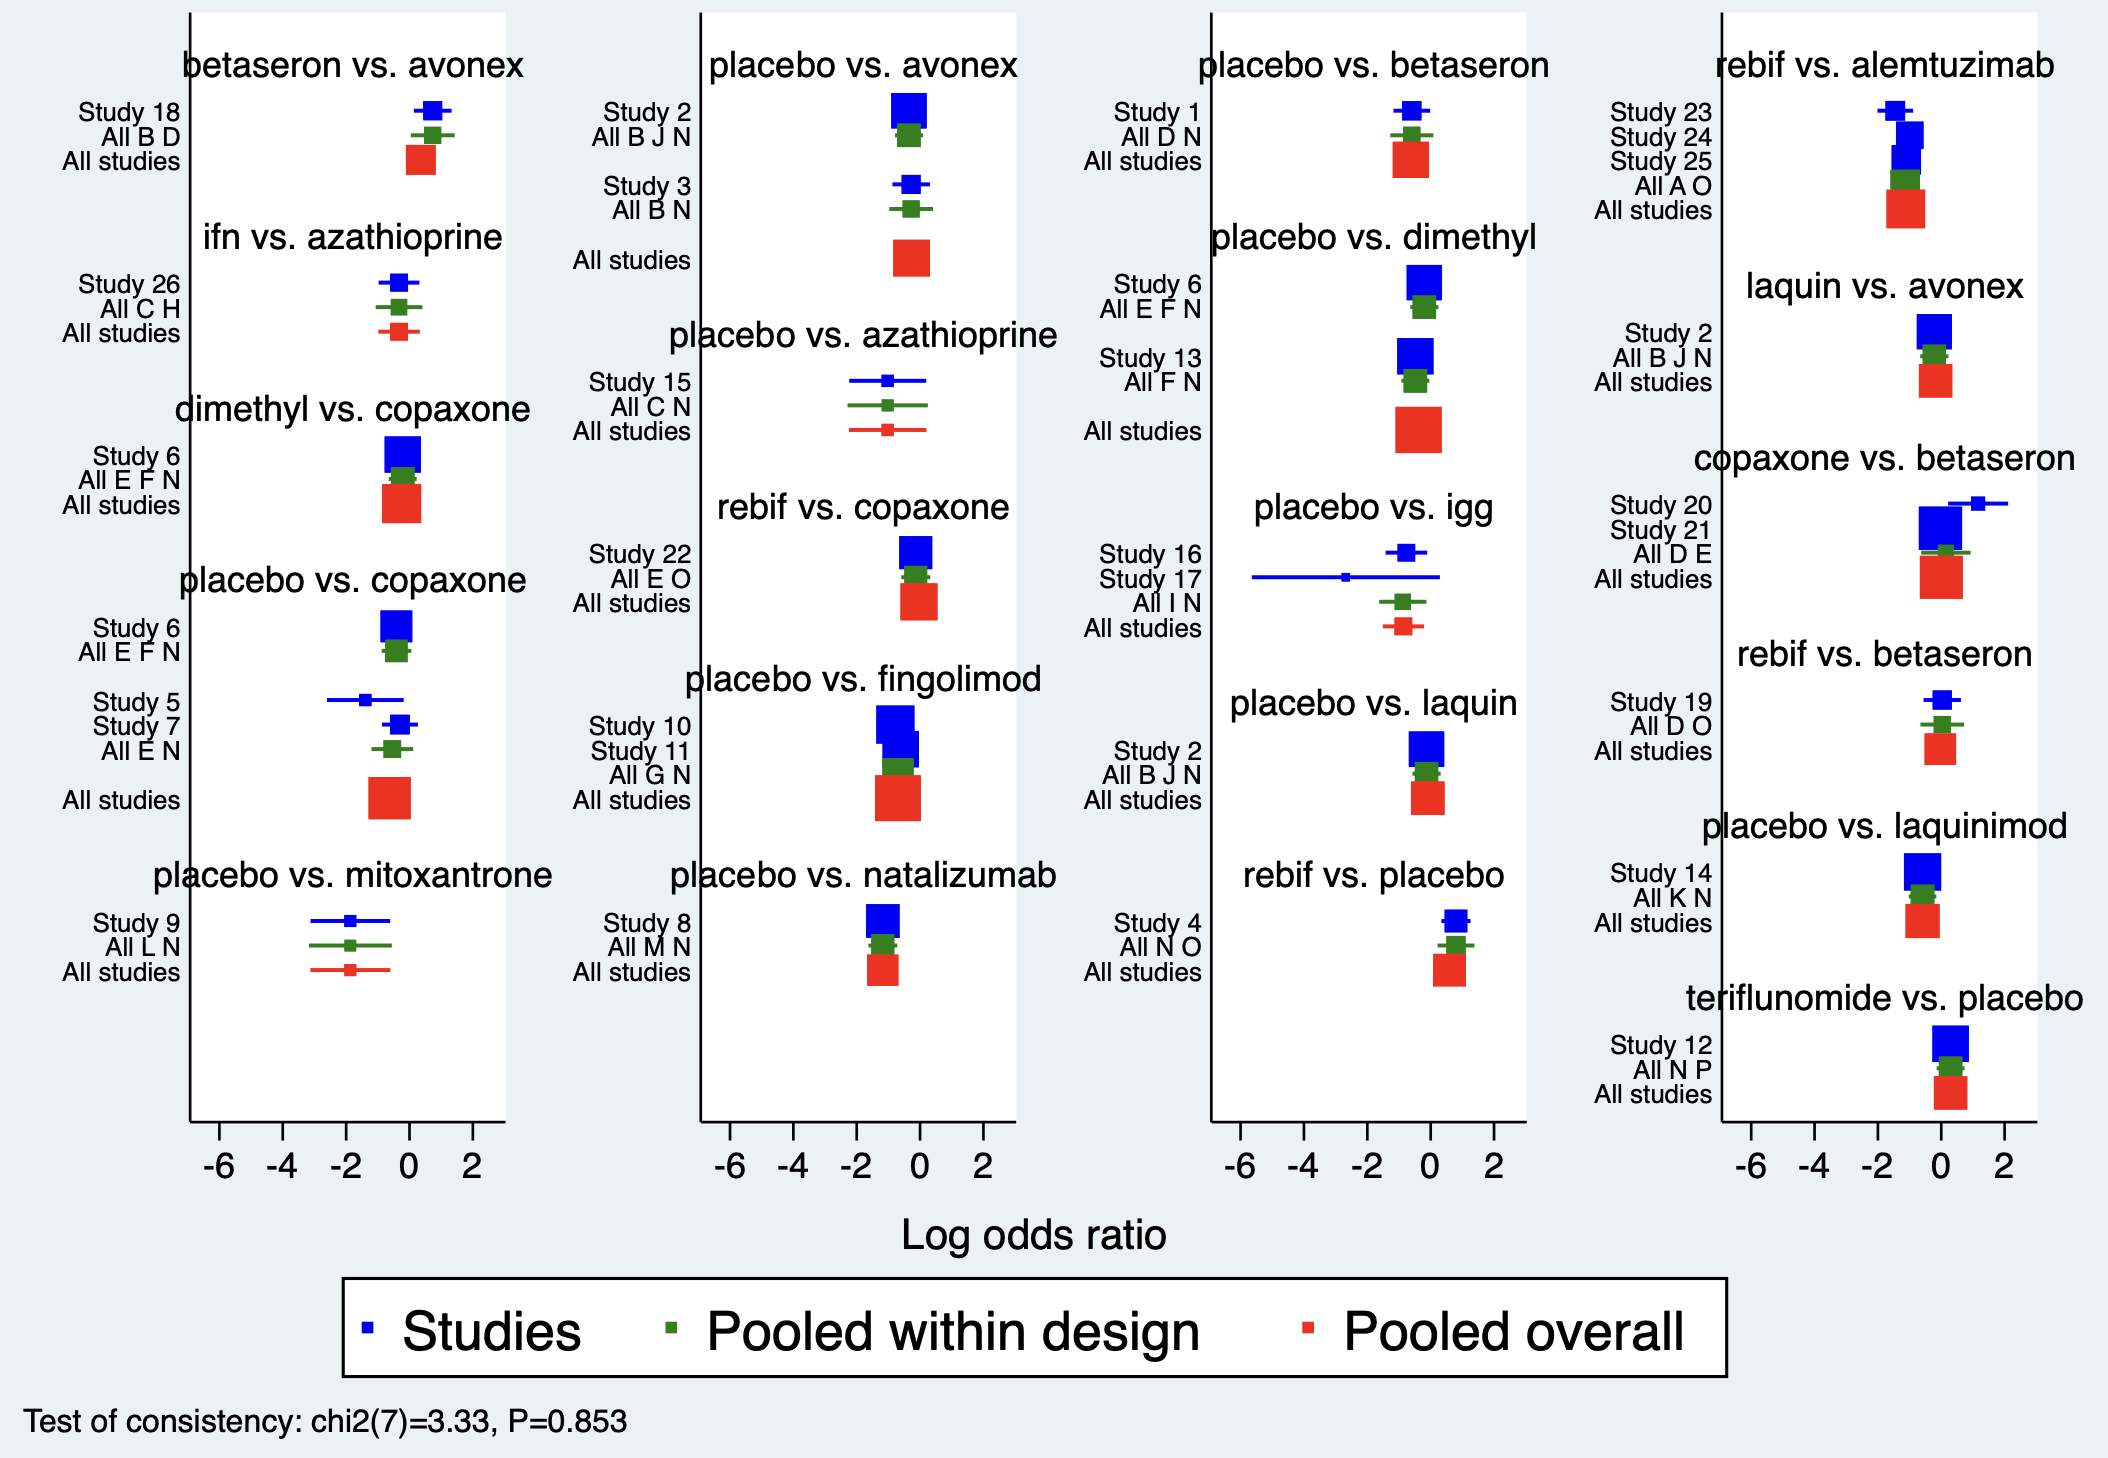
\includegraphics[width=1\linewidth,height=\textheight,keepaspectratio]{chapters/images/ch7-image7.png}

\textbf{代码7.7输出：直接证据与间接证据}

节点分裂模型亦可以用于分析网络荟萃分析的一致性，计算两个干预直接比较得出的参数和间接比较得出的参数。对这两个参数进行联合估计，比较它们的差值，检验其真实差值是否为0。直接证据与间接证据的一致性检验（含节点分裂法）可参见
Dias 等（2010）。

\begin{tcolorbox}[enhanced jigsaw, arc=.35mm, bottomrule=.15mm, breakable, colback=white, colframe=quarto-callout-note-color-frame, left=2mm, leftrule=.75mm, opacityback=0, rightrule=.15mm, toprule=.15mm]

\vspace{-3mm}\textbf{代码7.8}\vspace{3mm}

\begin{Shaded}
\begin{Highlighting}[]
\NormalTok{network sidesplit }\OtherTok{all}\NormalTok{, tau}
\end{Highlighting}
\end{Shaded}

\end{tcolorbox}

\begin{tcolorbox}[enhanced jigsaw, arc=.35mm, bottomrule=.15mm, breakable, colback=white, colframe=quarto-callout-note-color-frame, left=2mm, leftrule=.75mm, opacityback=0, rightrule=.15mm, toprule=.15mm]

\vspace{-3mm}\textbf{代码7.8输出}\vspace{3mm}

{\def\LTcaptype{none} % do not increment counter
\begin{longtable}[]{@{}
  >{\raggedright\arraybackslash}p{(\linewidth - 14\tabcolsep) * \real{0.1250}}
  >{\raggedright\arraybackslash}p{(\linewidth - 14\tabcolsep) * \real{0.1250}}
  >{\raggedright\arraybackslash}p{(\linewidth - 14\tabcolsep) * \real{0.1250}}
  >{\raggedright\arraybackslash}p{(\linewidth - 14\tabcolsep) * \real{0.1250}}
  >{\raggedright\arraybackslash}p{(\linewidth - 14\tabcolsep) * \real{0.1250}}
  >{\raggedright\arraybackslash}p{(\linewidth - 14\tabcolsep) * \real{0.1250}}
  >{\raggedright\arraybackslash}p{(\linewidth - 14\tabcolsep) * \real{0.1250}}
  >{\raggedright\arraybackslash}p{(\linewidth - 14\tabcolsep) * \real{0.1250}}@{}}
\toprule\noalign{}
\begin{minipage}[b]{\linewidth}\raggedright
Side
\end{minipage} & \begin{minipage}[b]{\linewidth}\raggedright
Direct
\end{minipage} & \begin{minipage}[b]{\linewidth}\raggedright
Indirect
\end{minipage} & \begin{minipage}[b]{\linewidth}\raggedright
Difference
\end{minipage} & \begin{minipage}[b]{\linewidth}\raggedright
\end{minipage} & \begin{minipage}[b]{\linewidth}\raggedright
\end{minipage} & \begin{minipage}[b]{\linewidth}\raggedright
\end{minipage} & \begin{minipage}[b]{\linewidth}\raggedright
\end{minipage} \\
\midrule\noalign{}
\endhead
\bottomrule\noalign{}
\endlastfoot
& Coef. & Std. Err. & Coef. & Std. Err. & Coef. & Std. Err. &
P\textgreater\textbar z\textbar{} \\
A O * & -1.11891 & .1216481 & .1276285 & 130.4523 & -1.246538 & 130.4525
& 0.992 \\
B D & .7341662 & .3086112 & .2096995 & .195126 & .5244667 & .3651234 &
0.151 \\
B J * & -.2187294 & .1507652 & .3397627 & .5260816 & -.5584921 &
.5472319 & 0.307 \\
B N * & -.3362652 & .1320421 & .1882035 & .341041 & -.5244687 & .3651335
& 0.151 \\
C H * & -.3296579 & .3343849 & 1.388427 & 1377.032 & -1.718085 &
1377.032 & 0.999 \\
C N * & -1.022072 & .6236976 & -2.108384 & 580.1129 & 1.086312 &
580.1133 & 0.999 \\
D E & .0736742 & .1684551 & -.1243108 & .2201667 & .197985 & .27642 &
0.474 \\
D N & -.594102 & .3058434 & -.629308 & .1518121 & .035206 & .3414485 &
0.918 \\
D O & .0312525 & .3104082 & -.0411736 & .18497 & .0724261 & .3613408 &
0.841 \\
E F & -.234583 & .1698999 & -.2847732 & .2478862 & .0501902 & .3039638 &
0.869 \\
E N & -.4351315 & .1326467 & -.8994905 & .1608528 & .464359 & .2093104 &
0.027 \\
E O & -.1361234 & .15271 & .152702 & .2075406 & -.2888254 & .2576693 &
0.262 \\
F N * & -.3441188 & .1070699 & -.8503738 & .4252508 & .506255 & .445895
& 0.256 \\
G N * & -.6985315 & .0999447 & -3.166373 & 930.055 & 2.467841 & 930.0551
& 0.998 \\
I N * & -.8591878 & .3328428 & -3.482589 & 1012.36 & 2.623401 & 1012.36
& 0.998 \\
J N * & -.1299553 & .1495573 & .4285362 & .527115 & -.5584915 & .547232
& 0.307 \\
K N * & -.5896181 & .1413525 & -3.396555 & 1028.739 & 2.806937 &
1028.739 & 0.998 \\
L N * & -1.865629 & .6443962 & -3.172957 & 1297.701 & 1.307328 &
1297.701 & 0.999 \\
M N * & -1.175059 & .1567734 & -3.090808 & 1407.469 & 1.915749 &
1407.469 & 0.999 \\
N O & .799673 & .2392806 & .4787151 & .1776051 & .320958 & .2979912 &
0.281 \\
N P * & .2954041 & .1444729 & 3.554453 & 1465.048 & -3.259049 & 1465.048
& 0.998 \\
* Warning: all the evidence about these contrasts comes from the trials
which directly compare them. & & & & & & & \\
\end{longtable}
}

\end{tcolorbox}

治疗效果修饰因素包括试验方法、临床特征，也可能包括随访时间、结果定义、研究质量（偏倚风险）、分析和报告标准（包括选择性报告的风险），这些都会影响网络荟萃分析的一致性。因此，在进行网络荟萃分析之前，重要的是只选择那些与临床关注人群相关的试验，然后确定这些试验中提供不同比较的任何系统性差异。

如果在节点分裂模型中发现不一致的证据，应寻求解释。例如，不一致是否来自于不同设计的特定研究或偏倚风险较高的研究。如果不一致仍然无法解释，那么可以将不一致项建模为均值为零的随机效应，这样就可以在考虑到无法解释的不一致的情况下进行总体的荟萃估计。

然而，网络荟萃分析亦存在不足之处。首先，SUCRA没有显示治疗之间的差异是否具有临床意义。虽然一种治疗可能被认为是最好的，但最好的治疗与其他治疗之间的绝对差异可能微不足道。其次，SUCRA的结果可能非常不准确，其95\%的可信区间极宽，在大多数的网络荟萃分析中，最佳治疗和次佳治疗之间没有真正的差异。第三，纳入非常多的研究，可能会分散人们对个别研究背后的事件和问题的注意力，如偏倚风险、方法的有效性和证据的质量。最后，网络荟萃分析要求强有力的假设，可传递性的假设难以论证，其得出的推论打破了临床试验的随机化，应该受到类似于观察性研究的限制。

\section{多结局的网络荟萃分析}\label{ux591aux7ed3ux5c40ux7684ux7f51ux7edcux835fux8403ux5206ux6790}

某一疾病的不同随机对照研究所感兴趣的结局变量可能不同。例如，在一项总结子宫内膜癌中孕酮受体状态预后效果的荟萃分析中，有四项研究提供了癌症特定生存期和无进展生存期的结果，但其他研究只提供了癌症特定生存期（两项研究）或无进展生存期（11项研究）的结果。如果只研究癌症特定生存期或只研究无进展生存期，则可能导致样本的浪费。多变量的网络元分析的统计模型通过同时分析多个结果和多个治疗来解决这个问题。这使得更多的研究能够为治疗的比较作出贡献。

Copas等提出，与试验间异质性程度相同的多变量网络荟萃分析相比，仅进行标准单变量荟萃分析，类似于丢掉了B\%的可用研究。

\textbf{公式7.2　B统计量}

\[B = 100\times(1 - E)\]

\textbf{公式7.3　信息效率}

\[E = \frac{\text{基于直接和间接证据汇总结果的方差}}{\text{仅基于直接证据汇总结果的方差}}\]

例如，如果E=0.9，那么标准的荟萃分析就类似于扔掉了10\%的可用研究。

B统计量提供了由间接证据产生荟萃结果的方差减少百分比。例如，在网络荟萃分析中，B为0\%表示结果只基于直接证据，而B为100\%表示完全基于间接证据。Riley等展示了如何为多结局荟萃分析模型推导出各项研究的权重。

当B统计量较大时，多结局荟萃分析有潜在重要性，特别是：报告感兴趣的结局的直接证据的研究占比不大；一些研究中感兴趣的结局没有报告，但报告了其他相关的结果；研究内或研究间，不同结局之间的相关程度很大（例如，\textgreater0.5或\textless-0.5）。

\section{前瞻性荟萃分析}\label{ux524dux77bbux6027ux835fux8403ux5206ux6790}

前瞻性荟萃分析（Prospective meta-analysis,
PMA），其最重要的特点是，纳入研究的结果发表之前就确定要把这些研究纳入到需要开展的荟萃分析中来，并先验的叙述需要做哪些统计分析。

有些临床问题可能需要大样本以确保足够的统计效率，但是单一中心的研究无法达到样本量。固然可以开展多中心研究，但由于经费、互相协调等因素，多中心随机对照研究并不可行，因此解决的方法就是在不同的机构开展多个类似的研究，在研究完成以后，再将其结果进行整合。第二种情况，研究人员在开展某项临床研究时，并不知道其他类似的实验正在进行，当研究过程中才得知这一情况，因此可以与其他正在进行类似研究的单位协作，并提前将计划整合到前瞻性荟萃分析中。

\textbf{案例7.3}

前瞻性荟萃分析可分为四个步骤。

第一步，确定需要使用前瞻性荟萃分析方法。研究问题是不是高度优先的，研究的问题有没有被解决，有没有新的研究涌现？如果没有新的正在开展的研究，也无法进行前瞻性的荟萃分析。如果开展常规的回顾性荟萃分析，能否达到同样的统计效能，如果能达到，也不需要用前瞻性荟萃分析来解决问题。

NeoProm是一个探索早产儿吸氧浓度和临床结局之间关系的研究，研究问题是高吸氧浓度是否增加早产儿死亡率。既往的研究多是观察性的，且根据这些研究的结局发生率计算出的样本量提示需要5000例早产儿才能检验出4\%的死亡率差别。单个机构无法达到这一样本量，而多中心研究受限于各中心的协调，经费问题，无法很好的开展。

PMA的第二步需要定义研究问题和纳入标准，并撰写研究方案。研究问题的定义按照PICO原则，需要再次强调的是，纳入标准的制定必须在研究结果发表之前。NeoProm研究中制定的受试者是出生后24小时之内的早产儿，干预组为是靶氧浓度为85-89\%，对照组靶氧浓度较高（91-95\%），结局事件是18到24个月龄的死亡和重大残疾的复合终点。

第三步是研究的检索，来源为临床研究注册的网站，Pubmed上发表的研究方案等。通过联系这些正在开展的随机对照研究的负责人组成了项目协作组。NeoProm研究中，协作组检索到了5个正在开展的RCT，各个单位独自开展了这个问题的随机对照研究，分别在澳大利亚、新西兰、加拿大、英国和美国进行，预计纳入将近5000例早产儿。前瞻性荟萃分析开始的时候，这五个研究的结果均还未发表。其他数据库的检索，也没有发现额外的其他研究。

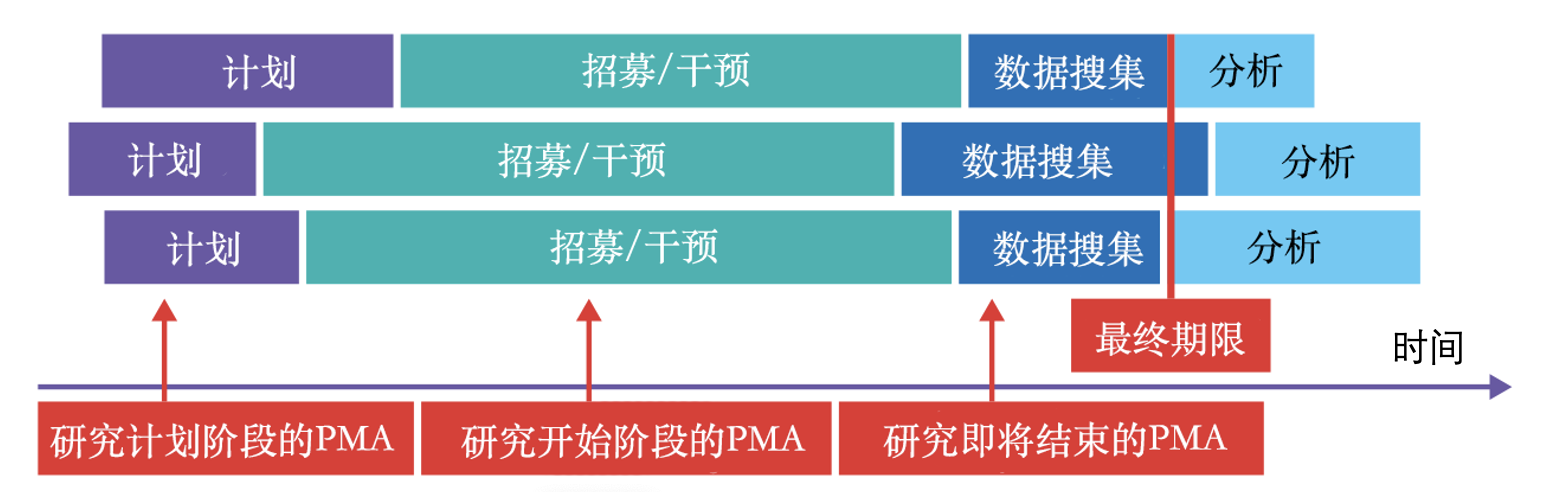
\includegraphics[width=1\linewidth,height=\textheight,keepaspectratio]{chapters/images/ch7-image8.png}

\textbf{图7.2 前瞻性荟萃分析图解}

第四步在PMA的开展过程中，还可以去协调各个子研究的计划，结局事件等。全部子研究的结果发表后，数据分析过程和常规的荟萃分析无区别。

\textbf{案例7.4}

世界卫生组织新冠肺炎疗法快速证据评估工作组发表了包括7项随机对照临床试验的前瞻性荟萃分析。

研究问题高度优先：皮质类固醇在治疗严重感染中的作用一直存在争议，这也导致新冠疫情的早期，关于皮质类固醇疗效的数据一直非常有限。

研究检索：据统计，截至2020年7月24日，全球范围内有55项皮质类固醇治疗新冠肺炎的研究在ClinicalTrials.gov上注册。世卫组织临床特征和管理工作组认识到获得可靠的皮质激素疗效数据以指导临床用药的紧迫性，因此制定了一项对正在进行的随机临床试验进行前瞻性荟萃分析的方案。几乎在世卫组织制定荟萃分析方案的同一时间，牛津大学团队领衔的大型临床研究RECOVERY的试验数据发布。这项试验中出现的明显获益信号，促使大多数正在开展的皮质类固醇研究停止招募。这也导致世卫组织最终只能纳入7项皮质类固醇治疗危重新冠肺炎患者的临床研究。

这7个临床研究招募的患者来自于澳大利亚、巴西、加拿大、中国、丹麦、法国、爱尔兰、荷兰、新西兰、西班牙、英国和美国。招募时间为2020年2月26日至2020年6月9日，最终随访日期为2020年7月6日。一共纳入1703名患者，其中678名患者接受皮质类固醇治疗（低剂量和高剂量的地塞米松、低剂量氢化可的松和高剂量甲泼尼龙），1025名患者接受常规治疗或安慰剂治疗。患者的中位年龄为60岁，488名（29\%）为女性。主要结局事件是随机化后28天的全因死亡率，次要结果是研究者定义的严重不良事件发生情况。

从总体上看，在678名使用皮质类固醇治疗的患者中，有222例死亡；在1025名使用常规治疗或安慰剂的患者中，有425例死亡。通过固定效应荟萃分析，比较皮质类固醇治疗的28天全因死亡率与常规治疗或安慰剂的28天全因死亡率，比值比为0.66。即使是排除RECOVERY研究的患者（因其结果发表早于前瞻性荟萃分析方案制定之前），研究结果也保持一致。

正是基于该项研究结果，世界卫生组织发布了使用皮质类固醇治疗新冠肺炎患者的指南。在这份指南中，世界卫生组织专家组强烈推荐危重新冠肺炎患者接受系统性皮质类固醇治疗，而不推荐在非重症新冠肺炎患者中使用皮质类固醇疗法。

\section{参考文献}\label{ux53c2ux8003ux6587ux732e-6}

\begin{enumerate}
\def\labelenumi{\arabic{enumi}.}
\item
  Riley RD, Jackson D, Salanti G, Burke DL, Price M, Kirkham J, White
  IR. Multivariate and network meta-analysis of multiple outcomes and
  multiple treatments: rationale, concepts, and examples. BMJ. 2017 Sep
  13;358:j3932.
\item
  Seidler AL, Hunter KE, Cheyne S, Ghersi D, Berlin JA, Askie L. A guide
  to prospective meta-analysis. BMJ. 2019 Oct 9;367:l5342.
\item
  Sterne JAC, Diaz J, Villar J, Murthy S, Slutsky AS, Perner A, Jüni P,
  Angus DC, Annane D, Azevedo LCP, Du B, Dequin PF, Gordon AC, Green C,
  Higgins JPT, Horby P, Landray MJ, Lapadula G, Le Gouge A, Leclerc M,
  Savović J, Tomazini B, Venkatesh B, Webb S, Marshall JC; WHO COVID-19
  Clinical Management and Characterization Working Group. Corticosteroid
  therapy for critically ill patients with COVID-19: A structured
  summary of a study protocol for a prospective meta-analysis of
  randomized trials. Trials. 2020 Aug 24;21(1):734.
\item
  Reitsma JB, Glas AS, Rutjes AW, et al.~Bivariate analysis of
  sensitivity and specificity produces informative summary measures in
  diagnostic reviews. Journal of Clinical Epidemiology, 2005,
  58(10):982-990.
\item
  Salanti G, Ades AE, Ioannidis JP. Graphical methods and numerical
  summaries for presenting results from multiple-treatment
  meta-analysis: an overview and tutorial. Journal of Clinical
  Epidemiology, 2011, 64(2):163-171.
\item
  Dias S, Welton NJ, Caldwell DM, Ades AE. Checking consistency in mixed
  treatment comparison meta-analysis. Statistics in Medicine, 2010,
  29(7-8):932-944.
\item
  Hutton B, Salanti G, Caldwell DM, et al.~The PRISMA extension
  statement for reporting of systematic reviews incorporating network
  meta-analyses of health care interventions: checklist and
  explanations. Annals of Internal Medicine, 2015, 162(11):777-784.
\item
  Salanti G. Indirect and mixed-treatment comparison, network, or
  multiple-treatments meta-analysis: many names, many benefits, many
  concerns for the next generation evidence synthesis tool. Research
  Synthesis Methods, 2012, 3(2):80-97.
\end{enumerate}

\bookmarksetup{startatroot}

\chapter{因果图与结构因果模型}\label{ux56e0ux679cux56feux4e0eux7ed3ux6784ux56e0ux679cux6a21ux578b}

本章开始介绍观察性研究中开展因果推断的理论知识与实践方法。

\section{因果有向无环图}\label{ux56e0ux679cux6709ux5411ux65e0ux73afux56fe}

数学概念中，图是节点和连接节点的边的集合。如果有一条从节点 𝑋 开始到节点
𝑌 结束的有向路径（箭头），那么可称 𝑋 是 𝑌 的祖先，𝑌 是 𝑋
的后代，即有向图的边从父节点到子节点。这条有向路径也代表了时间的流动，从某个节点
𝑋
出发回到自身的有向路径称为循环，这种发生时间旅行的情况不予考虑。通常考虑没有循环的情况，即有向图中没有环，称为有向无环图（Directed
Acyclic Graph，DAG）。

在因果有向无环图中，每个父节点都是其子节点的直接原因。如果改变 𝑋，𝑌
也能做出相应改变，称 𝑋 是 𝑌
的原因。因此，因果有向无环图中的边可视为因果关系。

因果有向无环图的一个重要假设是，因果有向无环图上的任何节点都是条件独立的，只依赖于其父节点。这个假设称为因果马尔可夫假设，意味着任何节点的共同父节点也必须包含在图中。这个假设其实是描述了两节点的相关性除了因果图中的显示，无其他隐藏的相关，与第一章中所描述的条件可交换性一致。

分叉与对撞是因果有向无环图中两个重要的结构。如果节点 \emph{S}
同时指向两个节点 \emph{X} 和 \emph{Y}，称为分叉结构；如果有两个节点
\emph{X} 和 \emph{Y} 同时指向节点
\emph{C}，称为对撞结构。在分叉结构中，\emph{X} 和 \emph{Y}
是非独立的，而对撞结构中 \emph{X} 和 \emph{Y} 是独立的。

因果图模型的局限性在于：

第一、因果图模型是一种非参数方法，既不指定因果关系的形式，也不描述关联程度的大小，是定性的分析工具。在因果图模型分析中，混杂因素可能会使结果产生偏差，但并没有对此偏差进行定量测度。

第二、因果图模型只有在背景信息完备时才是有效的，必须包含所有混杂因素，不存在未观察的混杂因素，才是准确的因果解释。因果有向无环图作为流行病学因果推断的工具，由
Greenland、Pearl 与 Robins（1999）系统引入；实践中可借助 DAGitty
等软件绘制因果图，并自动判定为识别因果效应所需控制的最小变量集（Textor
等，2016）。

\section{因果有向无环图的应用}\label{ux56e0ux679cux6709ux5411ux65e0ux73afux56feux7684ux5e94ux7528}

这是因果有向无环图的五个临床应用案例（图8.1）。

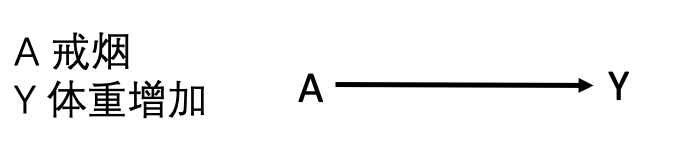
\includegraphics[width=2.90285in,height=\textheight,keepaspectratio]{chapters/images/ch8-image1.png}

\textbf{图8.1A}

\begin{enumerate}
\def\labelenumi{\arabic{enumi}.}
\tightlist
\item
  戒烟导致体重增加，\emph{A} 是 \emph{Y}
  的父节点，此图不存在任何其他节点。
\end{enumerate}

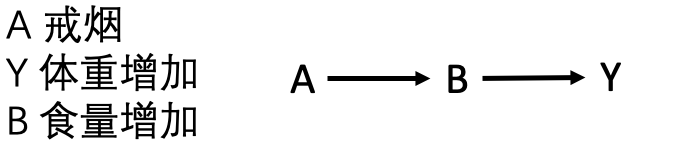
\includegraphics[width=2.90284in,height=\textheight,keepaspectratio]{chapters/images/ch8-image2.png}

\textbf{图8.1B}

\begin{enumerate}
\def\labelenumi{\arabic{enumi}.}
\setcounter{enumi}{1}
\tightlist
\item
  戒烟导致食量增加，继而食量增加再导致体重增加。食量增加是戒烟的子节点，又是体重增加的父节点。
\end{enumerate}

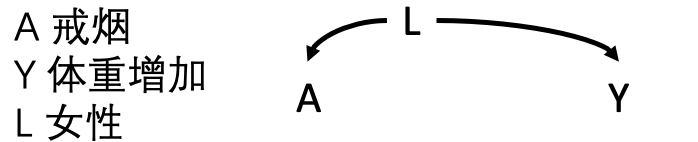
\includegraphics[width=2.90286in,height=\textheight,keepaspectratio]{chapters/images/ch8-image3.png}

\textbf{图8.1C}

\begin{enumerate}
\def\labelenumi{\arabic{enumi}.}
\setcounter{enumi}{2}
\tightlist
\item
  此为分叉结构，节点 \emph{L} 同时指向节点 \emph{A} 和
  \emph{Y。}女性可能戒烟比例高于男性，而女性在绝经期后体重增加比例较男性高。女性为戒烟和体重增加的共同原因，戒烟和体重增加非独立，两者通过性别产生关联。
\end{enumerate}

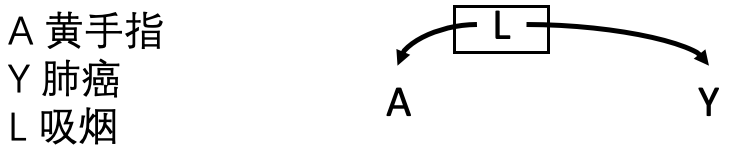
\includegraphics[width=2.9368in,height=\textheight,keepaspectratio]{chapters/images/ch8-image4.png}

\textbf{图8.1D}

\begin{enumerate}
\def\labelenumi{\arabic{enumi}.}
\setcounter{enumi}{3}
\tightlist
\item
  此为分叉结构，吸烟者大多出现手指变黄，而吸烟也有可引起肺癌。整个人群中，手指变黄与肺癌有关联。然而，当我们只考虑吸烟人群时，即吸烟节点上加框，黄手指和肺癌之间就相互独立。
\end{enumerate}

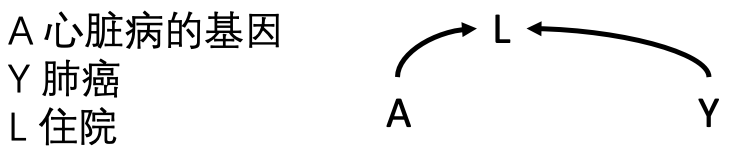
\includegraphics[width=2.93679in,height=\textheight,keepaspectratio]{chapters/images/ch8-image5.png}

\textbf{图8.1E}

\begin{enumerate}
\def\labelenumi{\arabic{enumi}.}
\setcounter{enumi}{4}
\tightlist
\item
  此为对撞结构，节点 \emph{A} 和 \emph{Y} 同时指向节点
  \emph{L。}携带心脏病的基因导致患者发生心脏病风险增高，住院比例增高；肺癌的发生也导致患者的住院风险增加。然而，携带心脏病的基因与肺癌相互独立。
\end{enumerate}

\section{后门准则与d-分离准则}\label{ux540eux95e8ux51c6ux5219ux4e0ed-ux5206ux79bbux51c6ux5219}

两个节点 𝑋 和 𝑌 之间的直接连接称为定向路径。除此之外，节点 𝑋 和节点 𝑌
之间还可能存在后门路径，即通过分叉结构，两个变量的共同父节点之间相互连接。两个变量如果通过对撞连接，在这种情况下，路径是封闭的。

研究者可以通过条件作用或控制一个变量，将路径的状态从开放状态变为封闭状态，或从封闭状态变为开放状态。条件作用或控制可以通过研究设计或统计方法（如限制、分层、匹配、标准化或多元回归）来实现。控制分叉结构的父节点可以关闭此后门路径，控制对撞结构的子节点会打开这条路径并导致非因果关联。

综上，因果有向无环图的使用有三大原则：

\begin{enumerate}
\def\labelenumi{\arabic{enumi}.}
\item
  节点 𝑋 和节点 𝑌 的因果关系只有在没有后门路径的情况下才成立；
\item
  阻断后门路径中的任一节点可以阻断该路径；
\item
  阻断对撞的子节点，可开放该路径。
\end{enumerate}

\section{前门准则}\label{ux524dux95e8ux51c6ux5219}

后门路径的存在导致无法直接对节点 𝑋 和节点 𝑌
的因果关系进行推断，虽然可以通过以上后门准则进行调整，但有时无法观察到后门路径上的节点。

此时，如果存在一个节点 \emph{M}，为节点 𝑋 的子节点和节点 𝑌
的父节点，这时可以通过前门调整的方法进行因果推断：

首先，估计节点 𝑋 对节点 \emph{M} 的因果效应，由于节点 𝑋 到节点 \emph{M}
不存在后门路径（对撞路径是封闭的）。

其次，估计节点 \emph{M} 对节点 \emph{Y} 的因果效应, 由于节点 \emph{M}
到节点 \emph{Y} 存在后门路径，但此路径可以通过调整 \emph{X} 进而阻断。

结合节点 𝑋 对节点 \emph{M} 和节点 M 对节点 \emph{Y} 的因果效应即为节点 𝑋
和节点 𝑌 的因果关系（图8.2）。


\includegraphics[width=4.1678in,height=\textheight,keepaspectratio]{chapters/images/ch8-image6.png}

\textbf{图8.2 前门准则}

因此，节点 \emph{M} 关于节点 𝑋 和节点 𝑌 满足前门准则，若：

\begin{enumerate}
\def\labelenumi{\arabic{enumi}.}
\item
  \emph{M} 完全中介了 \emph{X} 和 \emph{Y}，即所有从 \emph{X} 到
  \emph{Y} 的因果路径都经过 \emph{M}；
\item
  从 \emph{X} 到 \emph{M} 没有未被阻断的后门路径；
\item
  所有从 \emph{M} 到 \emph{Y} 没有未被阻断的后门路径。
\end{enumerate}

节点
\emph{M}符合中介因素的相关假设（详细参考第15章因果中介分析）。然而，不幸的是，前门准则鲜为应用，其原因为前门准则有着极其复杂的统计学假设，无法进行验证。后门准则、前门准则与
do 演算最早由
Pearl（1995）提出，构成了从因果图识别干预效应的完整理论框架。

\section{结构因果模型}\label{ux7ed3ux6784ux56e0ux679cux6a21ux578b}

结构因果模型（Structural Causal
Model，以下简称SCM）结合了上述介绍的图模型和虚拟事实模型，构建结构方程，并将其应用于因果分析。各类常用因果模型，都可以看作SCM的子类。结构因果模型中，用函数式的方程表示两个变量之间的因果关系：

\textbf{公式 8.1　结构方程}

\[Y = f(X, U)\]

其中，\emph{X} 和 \emph{Y}
是因果关系中的变量，即感兴趣的因与果，与计量经济学中的内生变量（endogenous
variable）对应。\emph{U}
表示其原因在感兴趣的因果模型外部，不对其建模，与计量经济学中的外生变量（exogenous
variable）对应。因而，结构因果模型是以下集合的数组：

\begin{enumerate}
\def\labelenumi{\arabic{enumi}.}
\item
  一组内生变量 \(`V`\)（包括\(`\ X`\) 和 \(`Y`\)）；
\item
  一组外生变量 \(`U`\)；
\item
  一组函数 \(`f`\)，输入其他变量可生成内生变量
\end{enumerate}

\(`f`\)
通常是一个线性函数，但是，当今大数据时代，此函数完全可以采用非线性函数、非参数模型。

结合本书第一章，结构方程模型提供了分类反事实关系的形式工具和符号机制。它刻画的是如下反事实``假设使
X = x，那么对于单个个体而言，在情形U时，Y 将会取的值''。

结构因果模型完全可以用因果图来表示，分别对应于结构方程中的内生变量与外生变量。请注意，外生变量
\emph{U}
只有由其出发的箭头，没有指向它的箭头。结构因果模型要求箭头表示箭头左侧项直接导致箭头右侧项（图8.3）。所以，在因果推断的过程中，必须按照因果箭头的方向进行推理，不能颠倒顺序。

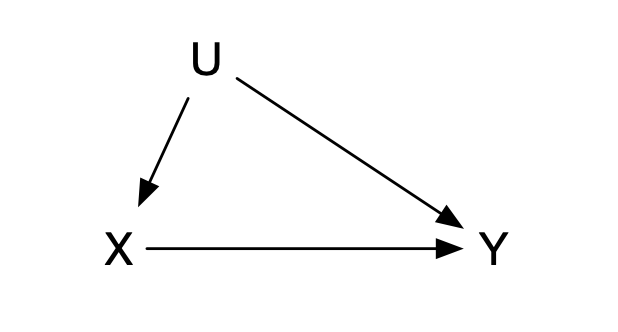
\includegraphics[width=2.93141in,height=\textheight,keepaspectratio]{chapters/images/ch8-image7.png}

\textbf{图8.3 结构因果模型中的外生变量与内生变量}

与因果有向无环图类似，结构因果模型的一个重要假设是马尔可夫假设，即某一变量只和直接影响它的变量有关，与其他变量都是独立的。结构因果模型不包含循环并且不存在未观察到的外生变量，则此因果模型符合马尔可夫假设；如果因果图不包含循环但存在未观察到的外生变量，则模型是半马尔可夫模型；非马尔可夫模型的因果图包含循环。

以上变量 \(`X`\)
是观察性研究中观察到的。随机对照研究中，研究某个干预对结局的影响，等同于在结构因果模型中，迫使一组变量
\(`X`\) 拥有值 \(`T`\)，只需将 \(`X\ `\)替换为
\(`T`\)。此时的因果图，由于干预是随机的，因此去除影响 𝑇 的所有因素。

结构因果模型也可进行反事实推理，即假如变量 \(`X`\) 拥有值 \(`T`\)
，\emph{Y} 会怎么样呢？我们对该模型进行干预，使得变量 \emph{X} 赋值为
\emph{T}；同时，我们观察到所有外生变量 \emph{U} 的值为
\emph{u}；在此情况下，我们向模型查询感兴趣变量 \emph{Y}
的条件概率。这种``干预（do 算子）---观测---反事实''的三层结构，正对应
Pearl
提出的因果之梯：结构因果模型为在三个层级之间进行形式化推理提供了统一的语言，也是机器学习走向因果推理的基础。

案例8.1

此例研究手术方法对某种肿瘤患者住院时长的影响，绘制其结构方程（图8.4）。根据临床知识，既能影响手术方法，又对住院时长有影响的因素包括技术、手术医生的经验、患者的偏好以及肿瘤的性质。这些因素皆为潜变量，以黄色标识。

很多医学研究中，经常会涉及到一些无法直接准确测量的变量，或不能以单一指标反映的变量，如工作满意度、医疗服务可及性、医疗服务满意性、健康状况、治疗偏好等。这类变量称为潜变量。一般可用一些可以观察到的指标，去间接替代这些潜变量。

此案例中，手术的年代可以反映技术的发展，手术医生的经验可以用年手术量来衡量、患者的偏好可能比较复杂（年龄、性别可能是一个潜在的影像因素），而肿瘤的性质包括肿瘤大小、侵袭性以及既往治疗史。

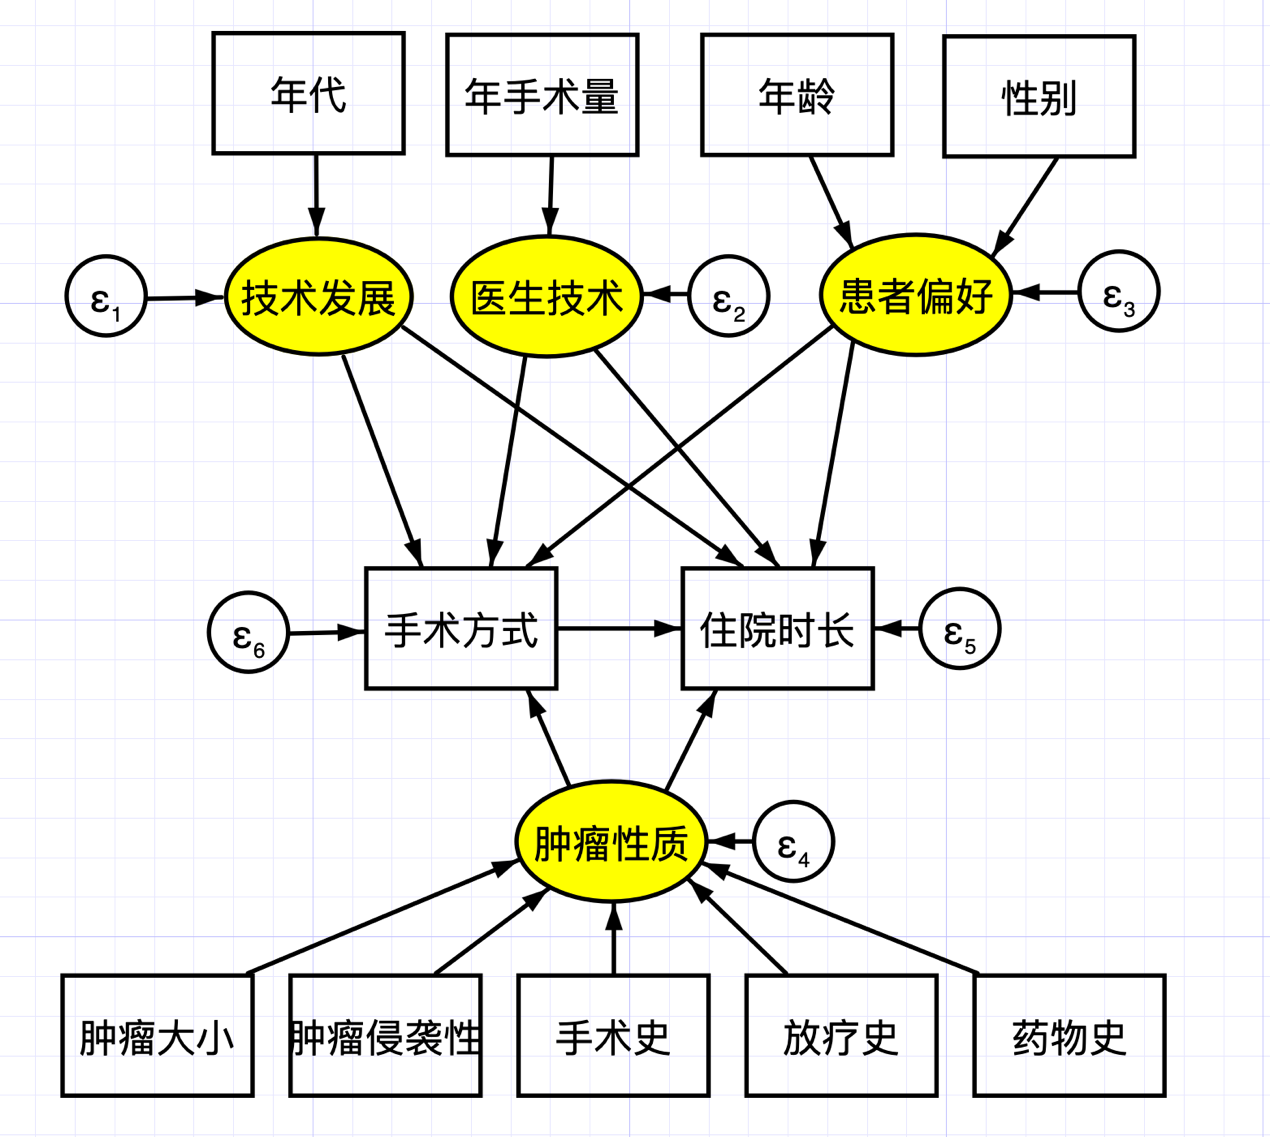
\includegraphics[width=5.76806in,height=\textheight,keepaspectratio]{chapters/images/ch8-image8.png}

\textbf{图8.4 结构方程}

\section{偏倚的分类}\label{ux504fux501aux7684ux5206ux7c7b}

研究者多使用偏倚来描述因果推断中的误差。但偏倚是一个比较笼统的概念，因果推断中的偏倚通常包括以下几个方面：

\begin{enumerate}
\def\labelenumi{\arabic{enumi}.}
\tightlist
\item
  混杂
\end{enumerate}

当治疗和结果有共同原因时，此共同原因会干扰治疗和结果之间的因果推断，许多流行病学家使用混淆/混杂一词来指代这种偏倚。这种类型的偏倚在因果有向无环图中表现为分叉结构，其中
\emph{L} 表示所有混杂因素的集合，如年龄，性别，疾病严重程度等。此图沿着
\emph{X} 到 \emph{Y} 有两条路径：一是直接从 \emph{X} 到 \emph{Y}
的有向路径（红色虚线）；二是从 \emph{X} 到 \emph{L} 再到 \emph{Y}
的后门路径（蓝色虚线）。如果要研究 \emph{X} 和 \emph{Y}
之间的因果关系，就必须阻断后门这条路径，即消除 L
的影响。因果图为混杂因素的选择提供了原则性依据：应调整能够阻断后门路径的变量，而切忌调整对撞因子或中介变量，否则反而会引入偏倚；混杂因素选择的形式化准则可参见
VanderWeele 与 Shpitser（2011）。

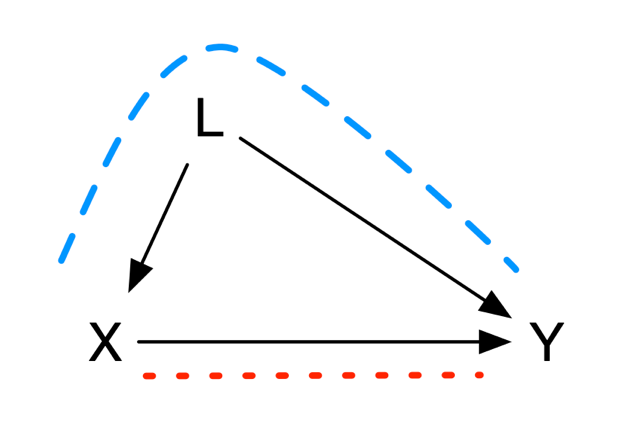
\includegraphics[width=2.92233in,height=\textheight,keepaspectratio]{chapters/images/ch8-image9.png}

\textbf{图8.5 混杂与后门路径}

健康工人偏倚：指从事某种职业（如消防员）的工人中观察到工人的总死亡率较一般人群低的现象。这是由于有严重疾病或缺陷的人不能从事某些职业所致，如不考虑这一效应，而将工人死亡率与一般人群死亡率相比是不合适的。

适应症混杂：某种药物（如阿司匹林）有很大可能开具给那些患有某些疾病的人（如心脏病），研究阿司匹林与心源性死亡率的关系时，患有心脏病既是治疗的原因，也是心源性死亡的危险因素。

生活方式：研究喝酒对死亡率的影响，喝酒这种生活方式往往与吸烟相关连，而吸烟与死亡率相关。其次、某种未发现的亚临床疾病可同时导致缺乏运动以及临床疾病风险增加。

遗传连锁不平衡：某两个基因位点存在遗传连锁不平衡性，这两个位点分别影响两种表型或者疾病的发展，因此会造成这两种表型或疾病的错误关联。

环境暴露：空气中的颗粒物对冠心病的影响可能会因为空气中存在其他污染物而产生混淆，空气中的颗粒物与其他污染物相关，而其他污染物可导致冠心病。

\begin{enumerate}
\def\labelenumi{\arabic{enumi}.}
\setcounter{enumi}{1}
\tightlist
\item
  选择偏倚
\end{enumerate}

控制了因和果的共同效果，许多流行病学家将其称为选择偏倚。选择偏倚是指被选择到研究样本中的患者同未进入样本中的患者之间存在着差异。这种类型的偏倚在因果有向无环图中表现为对撞结构，且阻断了其中的子节点，造成了原本关闭的路径重新开放。此图从
\emph{X} 到 \emph{Y} 的路径中又增加了一条从 \emph{X} 到 \emph{S} 再到
\emph{Y} 的后门路径。

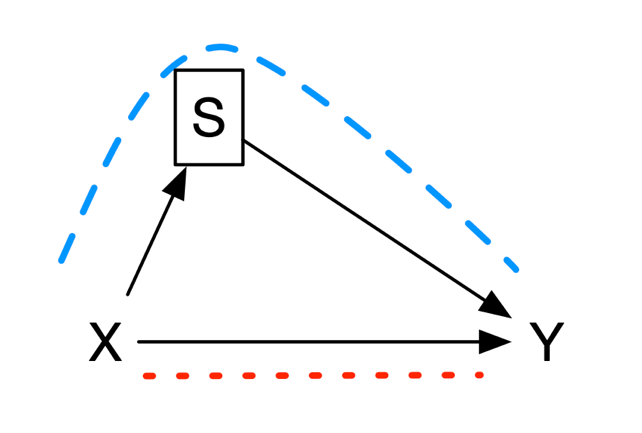
\includegraphics[width=2.92232in,height=\textheight,keepaspectratio]{chapters/images/ch8-image10.png}

\textbf{图8.6 选择偏倚与后门路径}

健康工人偏倚：在估计职业暴露与死亡率的影响时，只选择了在岗的工人，而忽略了因病请假的非在岗工人。

现患病偏倚：当研究的暴露因素与疾病预后相关，或暴露本身就是预后的决定因素，如果只研究现患病例的暴露状况。例如，以门诊和住院病例作为研究对象，欲探索某暴露与急性心肌梗塞的关系，如果该暴露因素可能引发病例的死亡，那么只选择住院和门诊病例会低估该因素的疾病风险。

同样，入院率偏倚是指选择医院病例为研究对象时，由于入院率的不同或就诊机会不同而导致入院率偏倚。例如，抢救不及时的死亡病例、距离较远的病例或病情轻的病例等。

病程长度偏倚：由于慢性疾病的病程长度不同，研究更容易纳入病程长的患者，恶性程度较高的患者可能因病程较短而死亡，并未被及时纳入研究，从而低估了结局风险。

研究开始前治疗的效果影响被选入研究的概率，如幸存者偏倚。这种偏倚可能存在于任何试图估计之前发生的治疗的因果效应的研究中。

失访偏倚是一种特殊的选择偏倚，指患者由于各种原因无法继续参加研究而退出，或研究人员无法获得患者的结局测量指标。治疗措施和研究的结局时间均能够影响失访与否。只计算随访病人中的因果效应会产生此偏倚。

尽管可以通过适当的研究设计来避免选择偏倚，但这通常不可避免。
例如，失访偏倚无法通过研究设计来避免。在这些情况下，选择偏差需要在统计分析中（逆概率加权或标准化）矫正。用因果图刻画选择偏倚的结构化方法可参见
Hernán、Hernández-Díaz 与 Robins（2004）；对撞偏倚的直观示例见 Cole
等（2010），其在大数据与人工智能研究中同样不容忽视（Griffith
等，2020）。

\begin{enumerate}
\def\labelenumi{\arabic{enumi}.}
\setcounter{enumi}{2}
\tightlist
\item
  测量误差
\end{enumerate}

另一个偏倚来源为测量误差。本书讨论的因果推断均假设所有变量------治疗、结果和协变量是完美测量的。然而，在实践中，测量会出现某种程度的错误。由测量误差引起的偏差称为测量偏差或信息偏差。

干预措施错分类：观察性研究中干预措施的信息一般通过医院电子病例系统、医保数据库、保险数据库等电子数据库识别提取，诸多因素可能导致错分类，导致实际接受干预者并非记录中的干预者。这些错分类往往只能作为潜在的研究缺陷，分析其对研究结论的影响。实际上，随机对照研究中的意向性分析也是一种干预措施错分类，随机化指定的干预措施不一定是受试者实际接受的干预。

结局错分类：识别结局指标通常依靠疾病诊断编码、程序算法以及一些数据提取系统，可能存在错分类。不同疾病ICD编码准确性也存在较大差异，例如，采用ICD-9诊断编码识别糖尿病的敏感性高达62.6\%；而识别急性心肌梗塞的敏感性仅为25.4\%。在生存结局研究中，采用总生存期为终点事件比较明确，发生结局错分的可能性较小；而采用无进展生存期则容易发生结局错分。

参考文献：

\begin{enumerate}
\def\labelenumi{\arabic{enumi}.}
\item
  Greenland S, Pearl J, Robins JM. Causal diagrams for epidemiologic
  research. Epidemiology, 1999, 10(1):37-48.
\item
  Pearl J. Causal diagrams for empirical research. Biometrika, 1995,
  82(4):669-688.
\item
  Hernán MA, Hernández-Díaz S, Robins JM. A structural approach to
  selection bias. Epidemiology, 2004, 15(5):615-625.
\item
  Cole SR, Platt RW, Schisterman EF, et al.~Illustrating bias due to
  conditioning on a collider. International Journal of Epidemiology,
  2010, 39(2):417-420.
\item
  VanderWeele TJ, Shpitser I. A new criterion for confounder selection.
  Biometrics, 2011, 67(4):1406-1413.
\item
  Textor J, van der Zander B, Gilthorpe MS, et al.~Robust causal
  inference using directed acyclic graphs: the R package `dagitty'.
  International Journal of Epidemiology, 2016, 45(6):1887-1894.
\item
  Griffith GJ, Morris TT, Tudball MJ, et al.~Collider bias undermines
  our understanding of COVID-19 disease risk and severity. Nature
  Communications, 2020, 11:5749.
\item
  Hernán MA, Robins JM (2020). Causal Inference: What If. Boca Raton:
  Chapman \& Hall/CRC.
\end{enumerate}

\bookmarksetup{startatroot}

\chapter{回归}\label{ux56deux5f52}

\section{结果回归}\label{ux7ed3ux679cux56deux5f52}

\begin{enumerate}
\def\labelenumi{\arabic{enumi}.}
\tightlist
\item
  连续型结局变量
\end{enumerate}

将上一章所述因果结构模型进一步细化，考虑 \(`f`\)
为线性函数，结局变量为连续变量，计算平均因果效应：

\textbf{公式 9.1　连续型结局的结果回归}

\[\begin{aligned}
Y &= f(X, U) \\
Y &= \beta_0 + \beta_1 X + \beta_2 U \\
E\!\left(Y^{X=1}\mid U\right)-E\!\left(Y^{X=0}\mid U\right) &= \beta_1
\end{aligned}\]

通过拟合结果回归模型，可以通过普通最小二乘法估计模型的参数。结果回归通过估计治疗的因果效应来调整混杂因素的每一层。如果变量
\(`\ U`\)
足以调整混杂（和选择偏倚）并且正确指定了该结构模型，则无需进一步需要调整。

\begin{enumerate}
\def\labelenumi{\arabic{enumi}.}
\setcounter{enumi}{1}
\tightlist
\item
  二分类结局变量
\end{enumerate}

当结局变量为分类变量（0或1）时，如果继续使用线性回归会导致\(`\ Y\ `\)的取值并不为0或1。逻辑回归（Logistic
regression）使用一个函数来归一化\(`\ Y\ `\)值，使\(`\ Y\ `\)的取值在区间（0,1）内，这个函数称为Logistic函数。逻辑回归本质上是线性回归，为了计算方便，引入比值这个概念（Odds），函数公式如下

\textbf{公式 9.2　二分类结局的逻辑回归}

\[\begin{aligned}
\Pr(Y=1\mid X,U) &= \operatorname{logit}^{-1}(\beta_0+\beta_1X+\beta_2U) \\
&= \frac{\exp(\beta_0+\beta_1X+\beta_2U)}{1+\exp(\beta_0+\beta_1X+\beta_2U)} \\
\operatorname{Odds}(Y^{X=1}) &= \exp(\beta_0+\beta_1+\beta_2U) \\
\operatorname{Odds}(Y^{X=0}) &= \exp(\beta_0+\beta_2U) \\
\operatorname{OR} &= \frac{\operatorname{Odds}(Y^{X=1})}{\operatorname{Odds}(Y^{X=0})}=\exp(\beta_1)
\end{aligned}\]

二分类变量的另一种因果效应描述方式是相对风险度（Risk
ratio，RR），定义为干预组发生结局事件的比例与非干预组发生结局事件的比例之比。当疾病的发病率\textless10\%时，RR与OR很接近。当发病率增大时，两者的差别增大，OR会高估
RR（详见 Zhang 与 Yu，1998）。

\textbf{公式 9.3　相对风险}

\[\operatorname{RR} = \frac{\Pr(Y^{X=1}=1)}{\Pr(Y^{X=0}=1)}\]

\begin{enumerate}
\def\labelenumi{\arabic{enumi}.}
\setcounter{enumi}{2}
\tightlist
\item
  二分类结局变量Probit模型
\end{enumerate}

又称为概率单元回归，最简单的Probit模型就是指结局变量 Y
为二分类变量，事件发生的概率是依赖于干预变量，\emph{f}
服从标准正态分布。当结局变量是分类变量时，逻辑回归和Probit回归没有本质的区别，一般情况下可以换用。区别在于采用的分布函数不同，前者假设随机变量服从逻辑概率分布，而后者假设随机变量服从正态分布。

\textbf{公式 9.4　二分类结局的 Probit 模型}

\[\Pr(Y=1\mid X,U) = \Phi(\beta_0+\beta_1X+\beta_2U)\]

回归系数一般情况下指的是干预变量每增加一个单位会导致结局事件发生的概率变化多少个单位，即概率密度函数的改变量，解释较逻辑回归麻烦。如果只有一个自变量
X，取值为 0 和 1 分别代表对照组和试验组，β0
代表就是对照组的概率单元值，β1
代表试验组与对照组的概率单元的差值。如果回归系数 β
为正，可解释为扣除其他因素的影响，该因素会使概率单元增加；如果为负值，则表示该因素会使概率单元减少。

案例9.1

生长激素型垂体腺瘤是一种过度分泌生长激素的垂体腺瘤，手术治疗是其主要治疗方法，目的是手术后的生长激素水平降至极低的水平。手术治疗包括使用内窥镜手术和显微镜手术两种方案。在回顾性数据中，纳入899例患者，观察到了如下表格中的数据。ID为患者标识；T代表手术方案，分别为内窥镜手术（Endoscopy）和显微镜手术（Microscopy）；K代表肿瘤侵袭性分级，指数越高，侵袭性越高；Y是感兴趣的结局事件；LOS是手术后的住院时长。

\textbf{案例9.1数据表}

{\def\LTcaptype{none} % do not increment counter
\begin{longtable}[]{@{}ccccc@{}}
\toprule\noalign{}
ID & T & K & Y & LOS \\
\midrule\noalign{}
\endhead
\bottomrule\noalign{}
\endlastfoot
\ldots{} & \ldots{} & \ldots{} & \ldots{} & \\
572 & Endoscopy & 3 & No & 5 \\
573 & Endoscopy & 0 & No & 8 \\
574 & Endoscopy & 3 & Yes & 6 \\
575 & Endoscopy & 3 & Yes & 6 \\
577 & Microscopy & 2 & Yes & 5 \\
578 & Microscopy & 0 & Yes & 6 \\
579 & Microscopy & 3 & No & 9 \\
\ldots{} & \ldots{} & \ldots{} & \ldots{} & \\
\end{longtable}
}

首先，根据临床先验知识，画出因果图（图9.1），研究不同的手术方法 T
是否影响手术后生长激素水平能否降至目标水平 Y。协变量为肿瘤的侵袭程度
K，在这个极其简化的模型中，假设调整 K
足以调整混杂（实际操作中可能存在其他因素，参见第8章），因此无需进一步调整其他因素，通过逻辑回归估计治疗
T 和结果 Y
之间的因果关系。回归结果比值比为2.32，95\%置信区间为1.64-3.28，p值0.000，即内窥镜组手术后生长激素降至目标水平的风险是显微镜组的2.32倍。其中，风险是指结局事件发生的可能性与不发生的可能性之比。

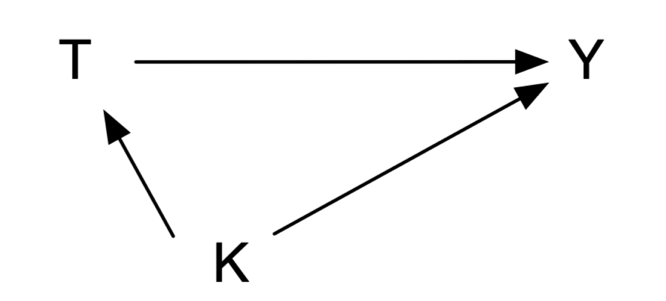
\includegraphics[width=2.93488in,height=\textheight,keepaspectratio]{chapters/images/ch9-image1.png}

\textbf{图9.1因果图}

\begin{tcolorbox}[enhanced jigsaw, arc=.35mm, bottomrule=.15mm, breakable, colback=white, colframe=quarto-callout-note-color-frame, left=2mm, leftrule=.75mm, opacityback=0, rightrule=.15mm, toprule=.15mm]

\vspace{-3mm}\textbf{代码9.1}\vspace{3mm}

\begin{Shaded}
\begin{Highlighting}[]
\KeywordTok{gen}\NormalTok{ Treatment = (t == }\StringTok{"Endoscopy"}\NormalTok{)}
\KeywordTok{gen}\NormalTok{ Outcome = 1 }\KeywordTok{if} \FunctionTok{y}\NormalTok{ == }\StringTok{"Yes"}
\KeywordTok{replace}\NormalTok{ Outcome = 0 }\KeywordTok{if} \FunctionTok{y}\NormalTok{ == }\StringTok{"No"}
\KeywordTok{logit}\NormalTok{ Outcome Treatment }\KeywordTok{k}\NormalTok{, }\KeywordTok{or}
\end{Highlighting}
\end{Shaded}

\end{tcolorbox}

\begin{tcolorbox}[enhanced jigsaw, arc=.35mm, bottomrule=.15mm, breakable, colback=white, colframe=quarto-callout-note-color-frame, left=2mm, leftrule=.75mm, opacityback=0, rightrule=.15mm, toprule=.15mm]

\vspace{-3mm}\textbf{代码9.1输出}\vspace{3mm}

{\def\LTcaptype{none} % do not increment counter
\begin{longtable}[]{@{}
  >{\centering\arraybackslash}p{(\linewidth - 6\tabcolsep) * \real{0.4875}}
  >{\raggedright\arraybackslash}p{(\linewidth - 6\tabcolsep) * \real{0.1875}}
  >{\centering\arraybackslash}p{(\linewidth - 6\tabcolsep) * \real{0.1750}}
  >{\centering\arraybackslash}p{(\linewidth - 6\tabcolsep) * \real{0.1500}}@{}}
\toprule\noalign{}
\begin{minipage}[b]{\linewidth}\centering
Logistic regression
\end{minipage} & \begin{minipage}[b]{\linewidth}\raggedright
Number of obs
\end{minipage} & \begin{minipage}[b]{\linewidth}\centering
=
\end{minipage} & \begin{minipage}[b]{\linewidth}\centering
\textbf{743}
\end{minipage} \\
\midrule\noalign{}
\endhead
\bottomrule\noalign{}
\endlastfoot
& LR chi2(2) & = & \textbf{167.81} \\
\textbf{Log pseudolikelihood = -430.27684} & Prob \textgreater{} chi2 &
= & \textbf{0.0000} \\
& Psudo R2 & = & \textbf{0.1632} \\
Outcome & Odds ratio & Std. err. & z \\
Treatment & \textbf{2.318421} & \textbf{.4086361} & \textbf{4.77} \\
k & \textbf{.4007459} & \textbf{.0324411} & \textbf{-11.30} \\
\_cons & \textbf{3.552514} & \textbf{.5975031} & \textbf{7.54} \\
\end{longtable}
}

\end{tcolorbox}

当然上述问题也可以采用Probit模型回归，其回归系数的解释就比较麻烦。模型截距=0.756，侵袭性的系数为-0.550，因此，侵袭性为1度时显微镜组（对照组，基线状态）的概率单元为0.756-0.550=0.206，干预变量的系数表示内窥镜组与显微镜组的概率单元值差值，概率单元值增加（0.497），即内窥镜组可增加疾病缓解的概率，结果具有统计学意义（p=0.000）。侵袭性为1度时内窥镜组的概率单元为0.206+0.497=0.703。

\begin{tcolorbox}[enhanced jigsaw, arc=.35mm, bottomrule=.15mm, breakable, colback=white, colframe=quarto-callout-note-color-frame, left=2mm, leftrule=.75mm, opacityback=0, rightrule=.15mm, toprule=.15mm]

\vspace{-3mm}\textbf{代码9.2}\vspace{3mm}

\begin{Shaded}
\begin{Highlighting}[]
\KeywordTok{probit}\NormalTok{ Outcome Treatment }\KeywordTok{k}
\end{Highlighting}
\end{Shaded}

\end{tcolorbox}

\begin{tcolorbox}[enhanced jigsaw, arc=.35mm, bottomrule=.15mm, breakable, colback=white, colframe=quarto-callout-note-color-frame, left=2mm, leftrule=.75mm, opacityback=0, rightrule=.15mm, toprule=.15mm]

\vspace{-3mm}\textbf{代码9.2输出}\vspace{3mm}

{\def\LTcaptype{none} % do not increment counter
\begin{longtable}[]{@{}
  >{\centering\arraybackslash}p{(\linewidth - 6\tabcolsep) * \real{0.4875}}
  >{\raggedright\arraybackslash}p{(\linewidth - 6\tabcolsep) * \real{0.1875}}
  >{\centering\arraybackslash}p{(\linewidth - 6\tabcolsep) * \real{0.1750}}
  >{\centering\arraybackslash}p{(\linewidth - 6\tabcolsep) * \real{0.1500}}@{}}
\toprule\noalign{}
\begin{minipage}[b]{\linewidth}\centering
Probit regression
\end{minipage} & \begin{minipage}[b]{\linewidth}\raggedright
Number of obs
\end{minipage} & \begin{minipage}[b]{\linewidth}\centering
=
\end{minipage} & \begin{minipage}[b]{\linewidth}\centering
\textbf{743}
\end{minipage} \\
\midrule\noalign{}
\endhead
\bottomrule\noalign{}
\endlastfoot
& LR chi2(2) & = & \textbf{167.48} \\
\textbf{Log pseudolikelihood = -430.44519} & Prob \textgreater{} chi2 &
= & \textbf{0.0000} \\
& Psudo R2 & = & \textbf{0.1629} \\
Outcome & Odds ratio & Std. err. & z \\
Treatment & \textbf{.4974691} & \textbf{.1038808} & \textbf{4.79} \\
k & \textbf{-.55001} & \textbf{.0457608} & \textbf{-12.02} \\
\_cons & \textbf{.7564864} & \textbf{.0978602} & \textbf{7.73} \\
\end{longtable}
}

\end{tcolorbox}

在Excel中可分别通过计算NORM.S.DIST (0.206, TRUE) 和 NORM.S.DIST (0.703,
TRUE)
，得出两者的累积分布函数值，分别为0.582和0.759。计算比值比为2.26，与逻辑回归接近。

\[\operatorname{OR}=\frac{0.759/(1-0.759)}{0.582/(1-0.582)}=2.26\]

其次，如果比较两种方案（内窥镜手术和显微镜手术）的住院时长，因其为连续变量，可采用线性回归计算。同样，为了简化，假设调整
K
足以调整混杂。回归系数为-0.62，95\%置信区间为-0.92至-0.32，p值0.000，表示内窥镜手术患者比显微镜手术患者平均住院时间少0.62天。

\begin{tcolorbox}[enhanced jigsaw, arc=.35mm, bottomrule=.15mm, breakable, colback=white, colframe=quarto-callout-note-color-frame, left=2mm, leftrule=.75mm, opacityback=0, rightrule=.15mm, toprule=.15mm]

\vspace{-3mm}\textbf{代码9.3}\vspace{3mm}

\begin{Shaded}
\begin{Highlighting}[]
\KeywordTok{reg}\NormalTok{ los Treatment }\KeywordTok{k}
\end{Highlighting}
\end{Shaded}

\end{tcolorbox}

\begin{tcolorbox}[enhanced jigsaw, arc=.35mm, bottomrule=.15mm, breakable, colback=white, colframe=quarto-callout-note-color-frame, left=2mm, leftrule=.75mm, opacityback=0, rightrule=.15mm, toprule=.15mm]

\vspace{-3mm}\textbf{代码9.3输出}\vspace{3mm}

{\def\LTcaptype{none} % do not increment counter
\begin{longtable}[]{@{}
  >{\raggedleft\arraybackslash}p{(\linewidth - 12\tabcolsep) * \real{0.1429}}
  >{\centering\arraybackslash}p{(\linewidth - 12\tabcolsep) * \real{0.1429}}
  >{\centering\arraybackslash}p{(\linewidth - 12\tabcolsep) * \real{0.1429}}
  >{\centering\arraybackslash}p{(\linewidth - 12\tabcolsep) * \real{0.1429}}
  >{\raggedright\arraybackslash}p{(\linewidth - 12\tabcolsep) * \real{0.1429}}
  >{\centering\arraybackslash}p{(\linewidth - 12\tabcolsep) * \real{0.1429}}
  >{\centering\arraybackslash}p{(\linewidth - 12\tabcolsep) * \real{0.1429}}@{}}
\toprule\noalign{}
\begin{minipage}[b]{\linewidth}\raggedleft
Source
\end{minipage} & \begin{minipage}[b]{\linewidth}\centering
SS
\end{minipage} & \begin{minipage}[b]{\linewidth}\centering
df
\end{minipage} & \begin{minipage}[b]{\linewidth}\centering
MS
\end{minipage} & \begin{minipage}[b]{\linewidth}\raggedright
Number of obs
\end{minipage} & \begin{minipage}[b]{\linewidth}\centering
=
\end{minipage} & \begin{minipage}[b]{\linewidth}\centering
\textbf{899}
\end{minipage} \\
\midrule\noalign{}
\endhead
\bottomrule\noalign{}
\endlastfoot
Model & \textbf{145.527971} & \textbf{2} & \textbf{72.763985} & F(3, 32)
& = & \textbf{14.86} \\
Residual & \textbf{4386.96146} & \textbf{896} & \textbf{4.8961623} &
Prob \textgreater{} F & = & \textbf{0.0000} \\
Total & \textbf{4532.48943} & \textbf{898} & \textbf{5.0473156} &
R-squared & = & \textbf{0.0321} \\
& & & & Adj R-squared & = & \textbf{0.0299} \\
& & & & Root MSE & = & \textbf{2.2127} \\
rate & Coefficient & Std. err. & t & P\textgreater\textbar t\textbar{} &
{[}95\% conf. interval{]} & \\
Treatment & \textbf{-.6208906} & \textbf{.1520286} & \textbf{-4.08} &
\textbf{0.000} & \textbf{-.91926} & \textbf{-.322517} \\
k & \textbf{.2791882} & \textbf{.0631276} & \textbf{4.42} &
\textbf{0.000} & \textbf{.155293} & \textbf{.4030834} \\
\_cons & \textbf{5.451714} & \textbf{.1435598} & \textbf{37.98} &
\textbf{0.000} & \textbf{5.16996} & \textbf{5.733467} \\
\end{longtable}
}

\end{tcolorbox}

\section{错误的回归方程}\label{ux9519ux8befux7684ux56deux5f52ux65b9ux7a0b}

结构因果模型中不应该阻断干预措施的子节点，即因果图上治疗 T
箭头所指向的变量（图9.2）。如果阻断了T的自变量，那可能会出现两种情况：或者阻断从
T 到 Y 的因果流动；或者在 T 和 Y 之间引入非因果关联。下图中，假设由治疗
T 到结局 Y 的因果流动是由变量 M
介导的，即内窥镜手术（T）增加生长激素达标率（Y）是因为增加了全切率（M）。此时，假设如果将分析限制在未全切的个体中（M
= 0）或全切的个体中（M =
1），用图中节点周围的方框表示。通过医学常识，未全切的患者生长激素水平肯定不能达标，这些患者中不管是否接受内窥镜治疗或显微镜治疗，手术都无法达标。因此，在M
=
0的个体中，治疗和结果无因果关系。这意味着如果阻断M，将削弱因果估计甚至将原本有统计意义的因果估计降为0。

确实，在将全切率纳入回归方程后，比值比降为1.17，比原先减少了49.6\%，95\%置信区间为0.79-1.74，p值0.441，没有统计学意义。需要注意的是，全切率
M 是 T 与 Y
之间的中介变量，将其纳入回归会阻断部分因果通路，从而低估总效应；这种对中介变量或对撞因子的不当调整称为过度调整偏倚（Schisterman
等，2009）。

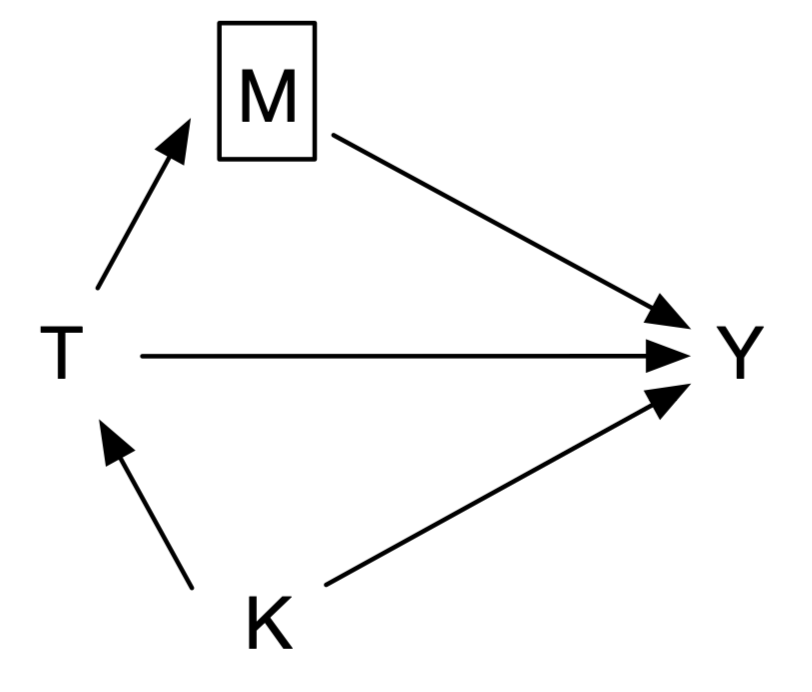
\includegraphics[width=2.3622in,height=\textheight,keepaspectratio]{chapters/images/ch9-image2.png}

\textbf{图9.2 错误的阻断干预的子节点：中介变量}

\begin{tcolorbox}[enhanced jigsaw, arc=.35mm, bottomrule=.15mm, breakable, colback=white, colframe=quarto-callout-note-color-frame, left=2mm, leftrule=.75mm, opacityback=0, rightrule=.15mm, toprule=.15mm]

\vspace{-3mm}\textbf{代码9.4}\vspace{3mm}

\begin{Shaded}
\begin{Highlighting}[]
\KeywordTok{gen}\NormalTok{ M = (extend == }\StringTok{"GTR"}\NormalTok{)}
\KeywordTok{logit}\NormalTok{ Outcome Treatment }\KeywordTok{k}\NormalTok{ M, }\KeywordTok{or}
\end{Highlighting}
\end{Shaded}

\end{tcolorbox}

\begin{tcolorbox}[enhanced jigsaw, arc=.35mm, bottomrule=.15mm, breakable, colback=white, colframe=quarto-callout-note-color-frame, left=2mm, leftrule=.75mm, opacityback=0, rightrule=.15mm, toprule=.15mm]

\vspace{-3mm}\textbf{代码9.4输出}\vspace{3mm}

{\def\LTcaptype{none} % do not increment counter
\begin{longtable}[]{@{}
  >{\centering\arraybackslash}p{(\linewidth - 6\tabcolsep) * \real{0.4875}}
  >{\raggedright\arraybackslash}p{(\linewidth - 6\tabcolsep) * \real{0.1875}}
  >{\centering\arraybackslash}p{(\linewidth - 6\tabcolsep) * \real{0.1750}}
  >{\centering\arraybackslash}p{(\linewidth - 6\tabcolsep) * \real{0.1500}}@{}}
\toprule\noalign{}
\begin{minipage}[b]{\linewidth}\centering
Logistic regression
\end{minipage} & \begin{minipage}[b]{\linewidth}\raggedright
Number of obs
\end{minipage} & \begin{minipage}[b]{\linewidth}\centering
=
\end{minipage} & \begin{minipage}[b]{\linewidth}\centering
\textbf{743}
\end{minipage} \\
\midrule\noalign{}
\endhead
\bottomrule\noalign{}
\endlastfoot
& LR chi2(2) & = & \textbf{308.30} \\
\textbf{Log pseudolikelihood = -360.03323} & Prob \textgreater{} chi2 &
= & \textbf{0.0000} \\
& Psudo R2 & = & \textbf{0.2998} \\
Outcome & Odds ratio & Std. err. & z \\
Treatment & \textbf{1.169176} & \textbf{.2374247} & \textbf{0.77} \\
k & \textbf{.6796318} & \textbf{.0652252} & \textbf{-4.02} \\
M & \textbf{18.40479} & \textbf{5.419085} & \textbf{9.89} \\
\_cons & \textbf{.197124} & \textbf{.0670321} & \textbf{-4.78} \\
\end{longtable}
}

\end{tcolorbox}

其次，如果 T 的后代变量又是 Y 的后代变量，即 T 和 Y 共同导致了
Z，此时如果以 Z 为条件，将导致 T 和 𝑌
之间出现非因果关联。这种情况通常发生在许多患者失访的情况下，研究者剔除了失访的患者，只关注有随访的患者，图9.3中C周围的方块表示以C=0为条件。如果治疗措施与失访相关（例如内窥镜是全新的治疗方式，因此研究者对内窥镜治疗的患者更加愿意随访，而显微镜治疗的患者失访率可能较高），而结局事件也可以影响失访率（如手术未全切，术后未达标的患者可能失访率较低）。此时，在失访的情况下，内窥镜治疗和显微镜治疗组可能差别不大，而单单分析未随访的患者可能夸大因果效应。

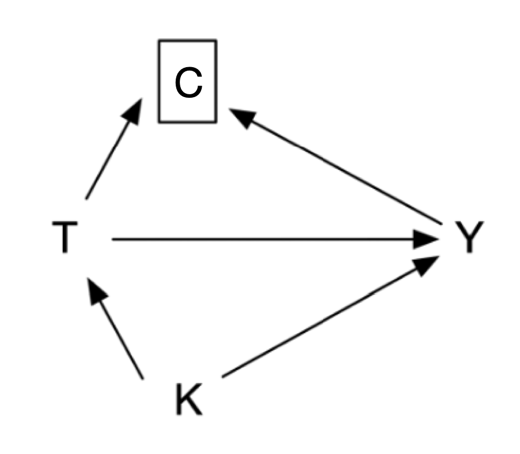
\includegraphics[width=2.3622in,height=\textheight,keepaspectratio]{chapters/images/ch9-image3.png}

\textbf{图9.3 错误的阻断干预的子节点：对撞变量}

\begin{tcolorbox}[enhanced jigsaw, arc=.35mm, bottomrule=.15mm, breakable, colback=white, colframe=quarto-callout-note-color-frame, left=2mm, leftrule=.75mm, opacityback=0, rightrule=.15mm, toprule=.15mm]

\vspace{-3mm}\textbf{代码9.5}\vspace{3mm}

\begin{Shaded}
\begin{Highlighting}[]
\KeywordTok{replace}\NormalTok{ Outcome = 1 }\KeywordTok{if} \FunctionTok{y}\NormalTok{ == }\StringTok{"Censored"}
\KeywordTok{logit}\NormalTok{ Outcome Treatment }\KeywordTok{k}\NormalTok{, }\KeywordTok{or}
\end{Highlighting}
\end{Shaded}

\end{tcolorbox}

\begin{tcolorbox}[enhanced jigsaw, arc=.35mm, bottomrule=.15mm, breakable, colback=white, colframe=quarto-callout-note-color-frame, left=2mm, leftrule=.75mm, opacityback=0, rightrule=.15mm, toprule=.15mm]

\vspace{-3mm}\textbf{代码9.5输出}\vspace{3mm}

{\def\LTcaptype{none} % do not increment counter
\begin{longtable}[]{@{}
  >{\centering\arraybackslash}p{(\linewidth - 6\tabcolsep) * \real{0.4810}}
  >{\raggedright\arraybackslash}p{(\linewidth - 6\tabcolsep) * \real{0.1899}}
  >{\centering\arraybackslash}p{(\linewidth - 6\tabcolsep) * \real{0.1772}}
  >{\centering\arraybackslash}p{(\linewidth - 6\tabcolsep) * \real{0.1519}}@{}}
\toprule\noalign{}
\begin{minipage}[b]{\linewidth}\centering
Logistic regression
\end{minipage} & \begin{minipage}[b]{\linewidth}\raggedright
Number of obs
\end{minipage} & \begin{minipage}[b]{\linewidth}\centering
=
\end{minipage} & \begin{minipage}[b]{\linewidth}\centering
\textbf{899}
\end{minipage} \\
\midrule\noalign{}
\endhead
\bottomrule\noalign{}
\endlastfoot
& LR chi2(2) & = & \textbf{175.80} \\
\textbf{Log pseudolikelihood = -527.0722} & Prob \textgreater{} chi2 & =
& \textbf{0.0000} \\
& Psudo R2 & = & \textbf{0.1429} \\
Outcome & Odds ratio & Std. err. & z \\
Treatment & \textbf{2.086615} & \textbf{.3299483} & \textbf{4.65} \\
k & \textbf{.427447} & \textbf{.0307782} & \textbf{-11.80} \\
\_cons & \textbf{4.908286} & \textbf{.7718278} & \textbf{10.12} \\
\end{longtable}
}

\end{tcolorbox}

在原始数据中内窥镜患者的失访率是16.7\%，显微镜患者的失访率是17.8\%，案例9.1的分析中将失访者排除在外进行因果推断。然而如果假设所有失访的患者都达标了，此时真正的因果效应是2.09，比案例9.1的结果减少了13.0\%。

\section{修饰效应}\label{ux4feeux9970ux6548ux5e94}

临床研究中的人群存在异质性，特定人群子集中的平均因果效应不一定与总体人群中的平均因果效应一致。不同生理情况的个体对治疗的敏感性不一。修饰效应的定义：当
T 与 Y 的平均因果效应在 V 的不同水平上存在差异时，即因子 V 改变了 T 与 Y
的关联强度， V 即为效应修饰因子。

\textbf{公式 9.5　效应修饰}

\[E\!\left(Y^{T=1}-Y^{T=0}\mid V=1\right) \ne E\!\left(Y^{T=1}-Y^{T=0}\mid V=0\right)\]

或在相对效应尺度上：

\[\frac{\Pr(Y^{T=1}=1\mid V=1)}{\Pr(Y^{T=0}=1\mid V=1)} \ne \frac{\Pr(Y^{T=1}=1\mid V=0)}{\Pr(Y^{T=0}=1\mid V=0)}\]

分层分析是识别修饰效应的常用方法。在变量 V 的每个级别（层）中计算 T 对 Y
的因果效应。计算过程分两步：① 根据不同的 V 分层；② 每个层中矫正混杂因素
L。文献中为了避免潜在的混淆，一些作者更喜欢使用术语``效应的跨层异质性''，实际上和修饰效应是同一概念。

案例9.1修饰效应

在上述数据中增加年龄变量Age。

案例9.1修饰效应数据表

{\def\LTcaptype{none} % do not increment counter
\begin{longtable}[]{@{}cccccc@{}}
\toprule\noalign{}
ID & Age & T & K & Y & LOS \\
\midrule\noalign{}
\endhead
\bottomrule\noalign{}
\endlastfoot
\ldots{} & \ldots{} & \ldots{} & \ldots{} & \ldots{} & \\
572 & 38 & Endoscopy & 3 & No & 5 \\
573 & 25 & Endoscopy & 0 & No & 8 \\
574 & 42 & Endoscopy & 3 & Yes & 6 \\
575 & 33 & Endoscopy & 3 & Yes & 6 \\
577 & 63 & Microscopy & 2 & Yes & 5 \\
578 & 52 & Microscopy & 0 & Yes & 6 \\
579 & 31 & Microscopy & 3 & No & 9 \\
\ldots{} & \ldots{} & \ldots{} & \ldots{} & \ldots{} & \\
\end{longtable}
}

分别在50岁及以下人群以及50岁以上人群中进行回归。

\begin{tcolorbox}[enhanced jigsaw, arc=.35mm, bottomrule=.15mm, breakable, colback=white, colframe=quarto-callout-note-color-frame, left=2mm, leftrule=.75mm, opacityback=0, rightrule=.15mm, toprule=.15mm]

\vspace{-3mm}\textbf{代码9.6}\vspace{3mm}

\begin{Shaded}
\begin{Highlighting}[]
\KeywordTok{logit}\NormalTok{ Outcome Treatment }\KeywordTok{k} \KeywordTok{if}\NormalTok{ age \textbackslash{}\textless{}= 50, }\KeywordTok{or}
\end{Highlighting}
\end{Shaded}

\end{tcolorbox}

\begin{tcolorbox}[enhanced jigsaw, arc=.35mm, bottomrule=.15mm, breakable, colback=white, colframe=quarto-callout-note-color-frame, left=2mm, leftrule=.75mm, opacityback=0, rightrule=.15mm, toprule=.15mm]

\vspace{-3mm}\textbf{代码9.6输出}\vspace{3mm}

{\def\LTcaptype{none} % do not increment counter
\begin{longtable}[]{@{}
  >{\centering\arraybackslash}p{(\linewidth - 6\tabcolsep) * \real{0.4875}}
  >{\raggedright\arraybackslash}p{(\linewidth - 6\tabcolsep) * \real{0.1875}}
  >{\centering\arraybackslash}p{(\linewidth - 6\tabcolsep) * \real{0.1750}}
  >{\centering\arraybackslash}p{(\linewidth - 6\tabcolsep) * \real{0.1500}}@{}}
\toprule\noalign{}
\begin{minipage}[b]{\linewidth}\centering
Logistic regression
\end{minipage} & \begin{minipage}[b]{\linewidth}\raggedright
Number of obs
\end{minipage} & \begin{minipage}[b]{\linewidth}\centering
=
\end{minipage} & \begin{minipage}[b]{\linewidth}\centering
\textbf{599}
\end{minipage} \\
\midrule\noalign{}
\endhead
\bottomrule\noalign{}
\endlastfoot
& LR chi2(2) & = & \textbf{137.52} \\
\textbf{Log pseudolikelihood = -346.29268} & Prob \textgreater{} chi2 &
= & \textbf{0.0000} \\
& Psudo R2 & = & \textbf{0.1657} \\
Outcome & Odds ratio & Std. err. & z \\
Treatment & \textbf{2.457885} & \textbf{.4822285} & \textbf{4.58} \\
k & \textbf{.4010976} & \textbf{.0360546} & \textbf{-10.16} \\
\_cons & \textbf{4.469598} & \textbf{.8864222} & \textbf{7.55} \\
\end{longtable}
}

\end{tcolorbox}

50岁以下人群中的比值比为2.46。

\begin{tcolorbox}[enhanced jigsaw, arc=.35mm, bottomrule=.15mm, breakable, colback=white, colframe=quarto-callout-note-color-frame, left=2mm, leftrule=.75mm, opacityback=0, rightrule=.15mm, toprule=.15mm]

\vspace{-3mm}\textbf{代码9.7}\vspace{3mm}

\begin{Shaded}
\begin{Highlighting}[]
\KeywordTok{logit}\NormalTok{ Outcome Treatment }\KeywordTok{k} \KeywordTok{if}\NormalTok{ age \textbackslash{}\textgreater{} 50, }\KeywordTok{or}
\end{Highlighting}
\end{Shaded}

\end{tcolorbox}

\begin{tcolorbox}[enhanced jigsaw, arc=.35mm, bottomrule=.15mm, breakable, colback=white, colframe=quarto-callout-note-color-frame, left=2mm, leftrule=.75mm, opacityback=0, rightrule=.15mm, toprule=.15mm]

\vspace{-3mm}\textbf{代码9.7输出}\vspace{3mm}

{\def\LTcaptype{none} % do not increment counter
\begin{longtable}[]{@{}
  >{\centering\arraybackslash}p{(\linewidth - 6\tabcolsep) * \real{0.4875}}
  >{\raggedright\arraybackslash}p{(\linewidth - 6\tabcolsep) * \real{0.1875}}
  >{\centering\arraybackslash}p{(\linewidth - 6\tabcolsep) * \real{0.1750}}
  >{\centering\arraybackslash}p{(\linewidth - 6\tabcolsep) * \real{0.1500}}@{}}
\toprule\noalign{}
\begin{minipage}[b]{\linewidth}\centering
Logistic regression
\end{minipage} & \begin{minipage}[b]{\linewidth}\raggedright
Number of obs
\end{minipage} & \begin{minipage}[b]{\linewidth}\centering
=
\end{minipage} & \begin{minipage}[b]{\linewidth}\centering
\textbf{300}
\end{minipage} \\
\midrule\noalign{}
\endhead
\bottomrule\noalign{}
\endlastfoot
& LR chi2(2) & = & \textbf{27.65} \\
\textbf{Log pseudolikelihood = -174.23677} & Prob \textgreater{} chi2 &
= & \textbf{0.0000} \\
& Psudo R2 & = & \textbf{0.0735} \\
Outcome & Odds ratio & Std. err. & z \\
Treatment & \textbf{1.37499} & \textbf{.3779807} & \textbf{1.16} \\
k & \textbf{.5332196} & \textbf{.0673594} & \textbf{-4.98} \\
\_cons & \textbf{5.39819} & \textbf{1.406641} & \textbf{6.47} \\
\end{longtable}
}

\end{tcolorbox}

50岁以上人群中的比值比为1.37，直观上两者存在明显差异，因此年龄可能是手术方式对内分泌预后的修饰效应因子。推断两者是否存在统计学差异请参考下一节边际效应。

研究者识别修饰效应因子有如下几个相关原因：

首先，如果一个因素改变了治疗对结果的影响，那么如果改变人群中该因素的占比，平均因果效应也将改变。假设某干预措施的结局的因果效应提示对女性有害，而对男性有益，如果选择一般人群（男女比1:1），则整个人群的平均因果效应为零。然而，如选择女性比例较高的人群中进行研究，则该人群的平均因果效应将变成有害。也就是说，人群总体中的平均因果效应取决于个体因果效应在总体中的分布。

在一个群体中计算的因果效应外推到第二个群体可能会缺乏可迁移性。本中心获得的因果效应可能在其他中心并不适用，因为两个中心的效应修饰因子分布不同。此外，不同中心还可能存在其他未测量或未知的因果效应修饰因子，这使得效应在人群间的可迁移性问题比因果关系识别问题更加困难。因此，因果效应的可迁移性是一个无法验证的假设，严重依赖学科知识。

其次，评估修饰效应的存在有助于识别能从干预中受益最多的群体。案例9.1中，手术方式对结果的平均因果效应在年龄较大的组中无统计学显著性。如果这个结论在多个中心的研究中得以证实，那么对于年龄较大的患者来说手术医生不会偏向任何方法，而对年轻患者来说手术医生会偏向内窥镜手术方法。

最后，效果修饰因子的识别可能有助于理解导致结果的生物学、社会学或其他机制。如，未割包皮的男性感染艾滋病毒的风险高于割包皮的男性可能会提供新的线索来了解这种疾病。术语修饰效应和交互作用有时在科学文献中用作同义词。但需指出，修饰效应（effect
modification）与交互作用（interaction）在概念上并不等同：前者关注在 V
的不同水平上 T 对 Y 效应的差异，并不要求 V 本身可干预；后者则赋予 T 与
T′ 同等的可干预地位。二者的严格区分可参见 VanderWeele（2009）。

\section{边际效应}\label{ux8fb9ux9645ux6548ux5e94}

所谓边际效应是从已有拟合模型结果中计算出来的统计量，该数值表示自变量的变化对结局变化的影响作用的大小。在对模型结果进行分析时，可以计算自变量取某一个值时，自变量对结局变量的边际值，也可以计算自变量平均值处的边际值，或者还可以计算其他变量取均值时某一自变量对结局变量的平均边际效应。这里边际值是指的结局变量的平均值或者平均概率，而边际效应是指干预组与对照组之间结局变量平均值或者平均概率之差。

边际效应采用的思想也是反事实框架下的思想，即假设所有样本的某一变量都取某一值，平均的结局指标是多少。这种``将某变量统一赋值、再求结局期望''的做法，本质上就是基于结果回归的标准化（g
公式）思想，是从回归模型估计平均因果效应的基础（Hernán 与
Robins，2020）。

案例9.1中计算手术、侵袭性以及年龄对生长激素达标的边际效应，利用margins命令，星号代表计算所有变量的边际效应

\begin{tcolorbox}[enhanced jigsaw, arc=.35mm, bottomrule=.15mm, breakable, colback=white, colframe=quarto-callout-note-color-frame, left=2mm, leftrule=.75mm, opacityback=0, rightrule=.15mm, toprule=.15mm]

\vspace{-3mm}\textbf{代码9.8}\vspace{3mm}

\begin{Shaded}
\begin{Highlighting}[]
\KeywordTok{logit}\NormalTok{ Outcome Treatment i.}\KeywordTok{k}\NormalTok{ age, }\KeywordTok{or}
\NormalTok{margins, }\KeywordTok{dydx}\NormalTok{(\textbackslash{}*)}
\end{Highlighting}
\end{Shaded}

\end{tcolorbox}

\begin{tcolorbox}[enhanced jigsaw, arc=.35mm, bottomrule=.15mm, breakable, colback=white, colframe=quarto-callout-note-color-frame, left=2mm, leftrule=.75mm, opacityback=0, rightrule=.15mm, toprule=.15mm]

\vspace{-3mm}\textbf{代码9.8输出}\vspace{3mm}

{\def\LTcaptype{none} % do not increment counter
\begin{longtable}[]{@{}
  >{\raggedright\arraybackslash}p{(\linewidth - 6\tabcolsep) * \real{0.4458}}
  >{\raggedright\arraybackslash}p{(\linewidth - 6\tabcolsep) * \real{0.1928}}
  >{\centering\arraybackslash}p{(\linewidth - 6\tabcolsep) * \real{0.1807}}
  >{\centering\arraybackslash}p{(\linewidth - 6\tabcolsep) * \real{0.1566}}@{}}
\toprule\noalign{}
\begin{minipage}[b]{\linewidth}\raggedright
Average marginal effects
\end{minipage} & \begin{minipage}[b]{\linewidth}\raggedright
Number of obs
\end{minipage} & \begin{minipage}[b]{\linewidth}\centering
=
\end{minipage} & \begin{minipage}[b]{\linewidth}\centering
\textbf{743}
\end{minipage} \\
\midrule\noalign{}
\endhead
\bottomrule\noalign{}
\endlastfoot
Model VCE: OIM & & & \\
Expression: Pr(Outcome), predict()

dy/dx wrt: Treatment k age & & & \\
& & & \\
& Delta-method & & \\
Margin & Std. err. & z & P\textgreater\textbar z\textbar{} \\
Treatment & \textbf{.1602185} & \textbf{.0329159} & \textbf{4.87} \\
k & \textbf{-.1746125} & \textbf{.0105929} & \textbf{-16.48} \\
age & \textbf{.0030562} & \textbf{.0013536} & \textbf{2.26} \\
\end{longtable}
}

\end{tcolorbox}

平均边际效应提示保持其他变量不变，从显微镜组至内窥镜组内分泌缓解率平均增加16.0\%；保持其他变量不变，侵袭性每增加一个级别内分泌缓解率平均减少17.5\%。保持其他变量不变，年龄每增加十岁，内分泌缓解率平均增加3.1\%。可以绘制平均边际值随侵袭性变化（分类变量）以及随年龄变化（连续变量）的曲线。

\begin{tcolorbox}[enhanced jigsaw, arc=.35mm, bottomrule=.15mm, breakable, colback=white, colframe=quarto-callout-note-color-frame, left=2mm, leftrule=.75mm, opacityback=0, rightrule=.15mm, toprule=.15mm]

\vspace{-3mm}\textbf{代码9.9}\vspace{3mm}

\begin{Shaded}
\begin{Highlighting}[]
\NormalTok{margins, }\KeywordTok{dydx}\NormalTok{(}\KeywordTok{k}\NormalTok{)}
\NormalTok{marginsplot}
\end{Highlighting}
\end{Shaded}

\end{tcolorbox}

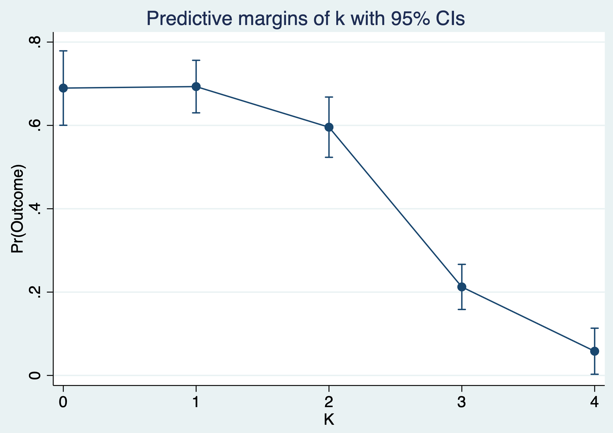
\includegraphics[width=5.76772in,height=\textheight,keepaspectratio]{chapters/images/ch9-image4.png}

\textbf{代码9.9输出缓解率（纵轴）随侵袭性（横轴）变化}

\begin{tcolorbox}[enhanced jigsaw, arc=.35mm, bottomrule=.15mm, breakable, colback=white, colframe=quarto-callout-note-color-frame, left=2mm, leftrule=.75mm, opacityback=0, rightrule=.15mm, toprule=.15mm]

\vspace{-3mm}\textbf{代码9.10}\vspace{3mm}

\begin{Shaded}
\begin{Highlighting}[]
\NormalTok{marginscontplot age, }\KeywordTok{ci}
\end{Highlighting}
\end{Shaded}

\end{tcolorbox}

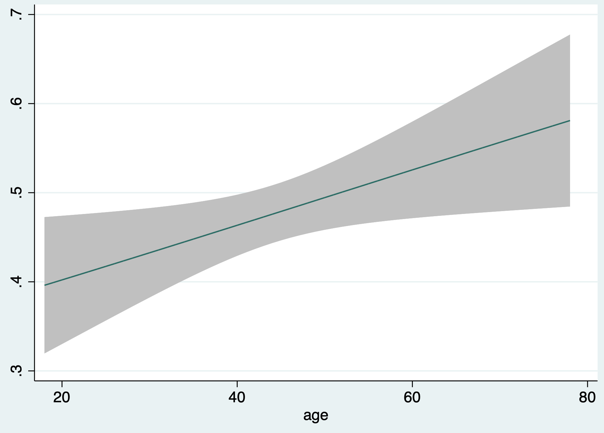
\includegraphics[width=5.76772in,height=\textheight,keepaspectratio]{chapters/images/ch9-image5.png}

\textbf{代码9.10输出缓解率（纵轴）随年龄（横轴）变化}

本章第一节已知内窥镜干预能提高手术缓解率。然而，侵袭性亦会影响手术效果。因此，我们想探究侵袭性能否调节干预对手术缓解率的影响作用。于是，在回归模型中加入这两个变量的交乘项来检验修饰效应。

\begin{tcolorbox}[enhanced jigsaw, arc=.35mm, bottomrule=.15mm, breakable, colback=white, colframe=quarto-callout-note-color-frame, left=2mm, leftrule=.75mm, opacityback=0, rightrule=.15mm, toprule=.15mm]

\vspace{-3mm}\textbf{代码9.11}\vspace{3mm}

\begin{Shaded}
\begin{Highlighting}[]
\KeywordTok{logit}\NormalTok{ Outcome i.Treatment }\KeywordTok{k}\NormalTok{ i.Treatment\#c.}\KeywordTok{k}\NormalTok{ age, }\KeywordTok{or}
\NormalTok{margins }\KeywordTok{k}\NormalTok{, }\KeywordTok{dydx}\NormalTok{(i.Treatment) plot}
\end{Highlighting}
\end{Shaded}

\end{tcolorbox}

\begin{tcolorbox}[enhanced jigsaw, arc=.35mm, bottomrule=.15mm, breakable, colback=white, colframe=quarto-callout-note-color-frame, left=2mm, leftrule=.75mm, opacityback=0, rightrule=.15mm, toprule=.15mm]

\vspace{-3mm}\textbf{代码9.11输出}\vspace{3mm}

{\def\LTcaptype{none} % do not increment counter
\begin{longtable}[]{@{}
  >{\centering\arraybackslash}p{(\linewidth - 6\tabcolsep) * \real{0.4875}}
  >{\raggedright\arraybackslash}p{(\linewidth - 6\tabcolsep) * \real{0.1875}}
  >{\centering\arraybackslash}p{(\linewidth - 6\tabcolsep) * \real{0.1750}}
  >{\centering\arraybackslash}p{(\linewidth - 6\tabcolsep) * \real{0.1500}}@{}}
\toprule\noalign{}
\begin{minipage}[b]{\linewidth}\centering
Logistic regression
\end{minipage} & \begin{minipage}[b]{\linewidth}\raggedright
Number of obs
\end{minipage} & \begin{minipage}[b]{\linewidth}\centering
=
\end{minipage} & \begin{minipage}[b]{\linewidth}\centering
\textbf{743}
\end{minipage} \\
\midrule\noalign{}
\endhead
\bottomrule\noalign{}
\endlastfoot
& LR chi2(2) & = & \textbf{174.92} \\
\textbf{Log pseudolikelihood = -426.72345} & Prob \textgreater{} chi2 &
= & \textbf{0.0000} \\
& Psudo R2 & = & \textbf{0.1701} \\
Outcome & Odds ratio & Std. err. & z \\
1.Treatment & \textbf{3.650757} & \textbf{1.391229} & \textbf{3.40} \\
k & \textbf{.4529654} & \textbf{.0472107} & \textbf{-7.60} \\
Treatment\#c.k 1 & \textbf{.7861221} & \textbf{.1317911} &
\textbf{-1.44} \\
age & \textbf{1.015891} & \textbf{.0071311} & \textbf{2.25} \\
\_cons & \textbf{1.467374} & \textbf{.555727} & \textbf{1.01} \\
\end{longtable}
}

\end{tcolorbox}

回归模型中，交乘项的系数p值大于0.05，提示统计学分析不提示侵袭性是手术效果的修饰效应。然而，应该注意到样本量与统计效能的问题。更加直观的方法是计算不同侵袭性级别肿瘤中的边际效应，可见级别为0-3的肿瘤中，边际效应均为正值，级别为4的肿瘤边际效应接近零，95\%区间有重叠。

\begin{tcolorbox}[enhanced jigsaw, arc=.35mm, bottomrule=.15mm, breakable, colback=white, colframe=quarto-callout-note-color-frame, left=2mm, leftrule=.75mm, opacityback=0, rightrule=.15mm, toprule=.15mm]

\vspace{-3mm}\textbf{代码9.12}\vspace{3mm}

\begin{Shaded}
\begin{Highlighting}[]
\NormalTok{margins, }\KeywordTok{dydx}\NormalTok{(Treatment) }\FunctionTok{at}\NormalTok{(}\KeywordTok{k}\NormalTok{=(0(1)4)) plot}
\end{Highlighting}
\end{Shaded}

\end{tcolorbox}

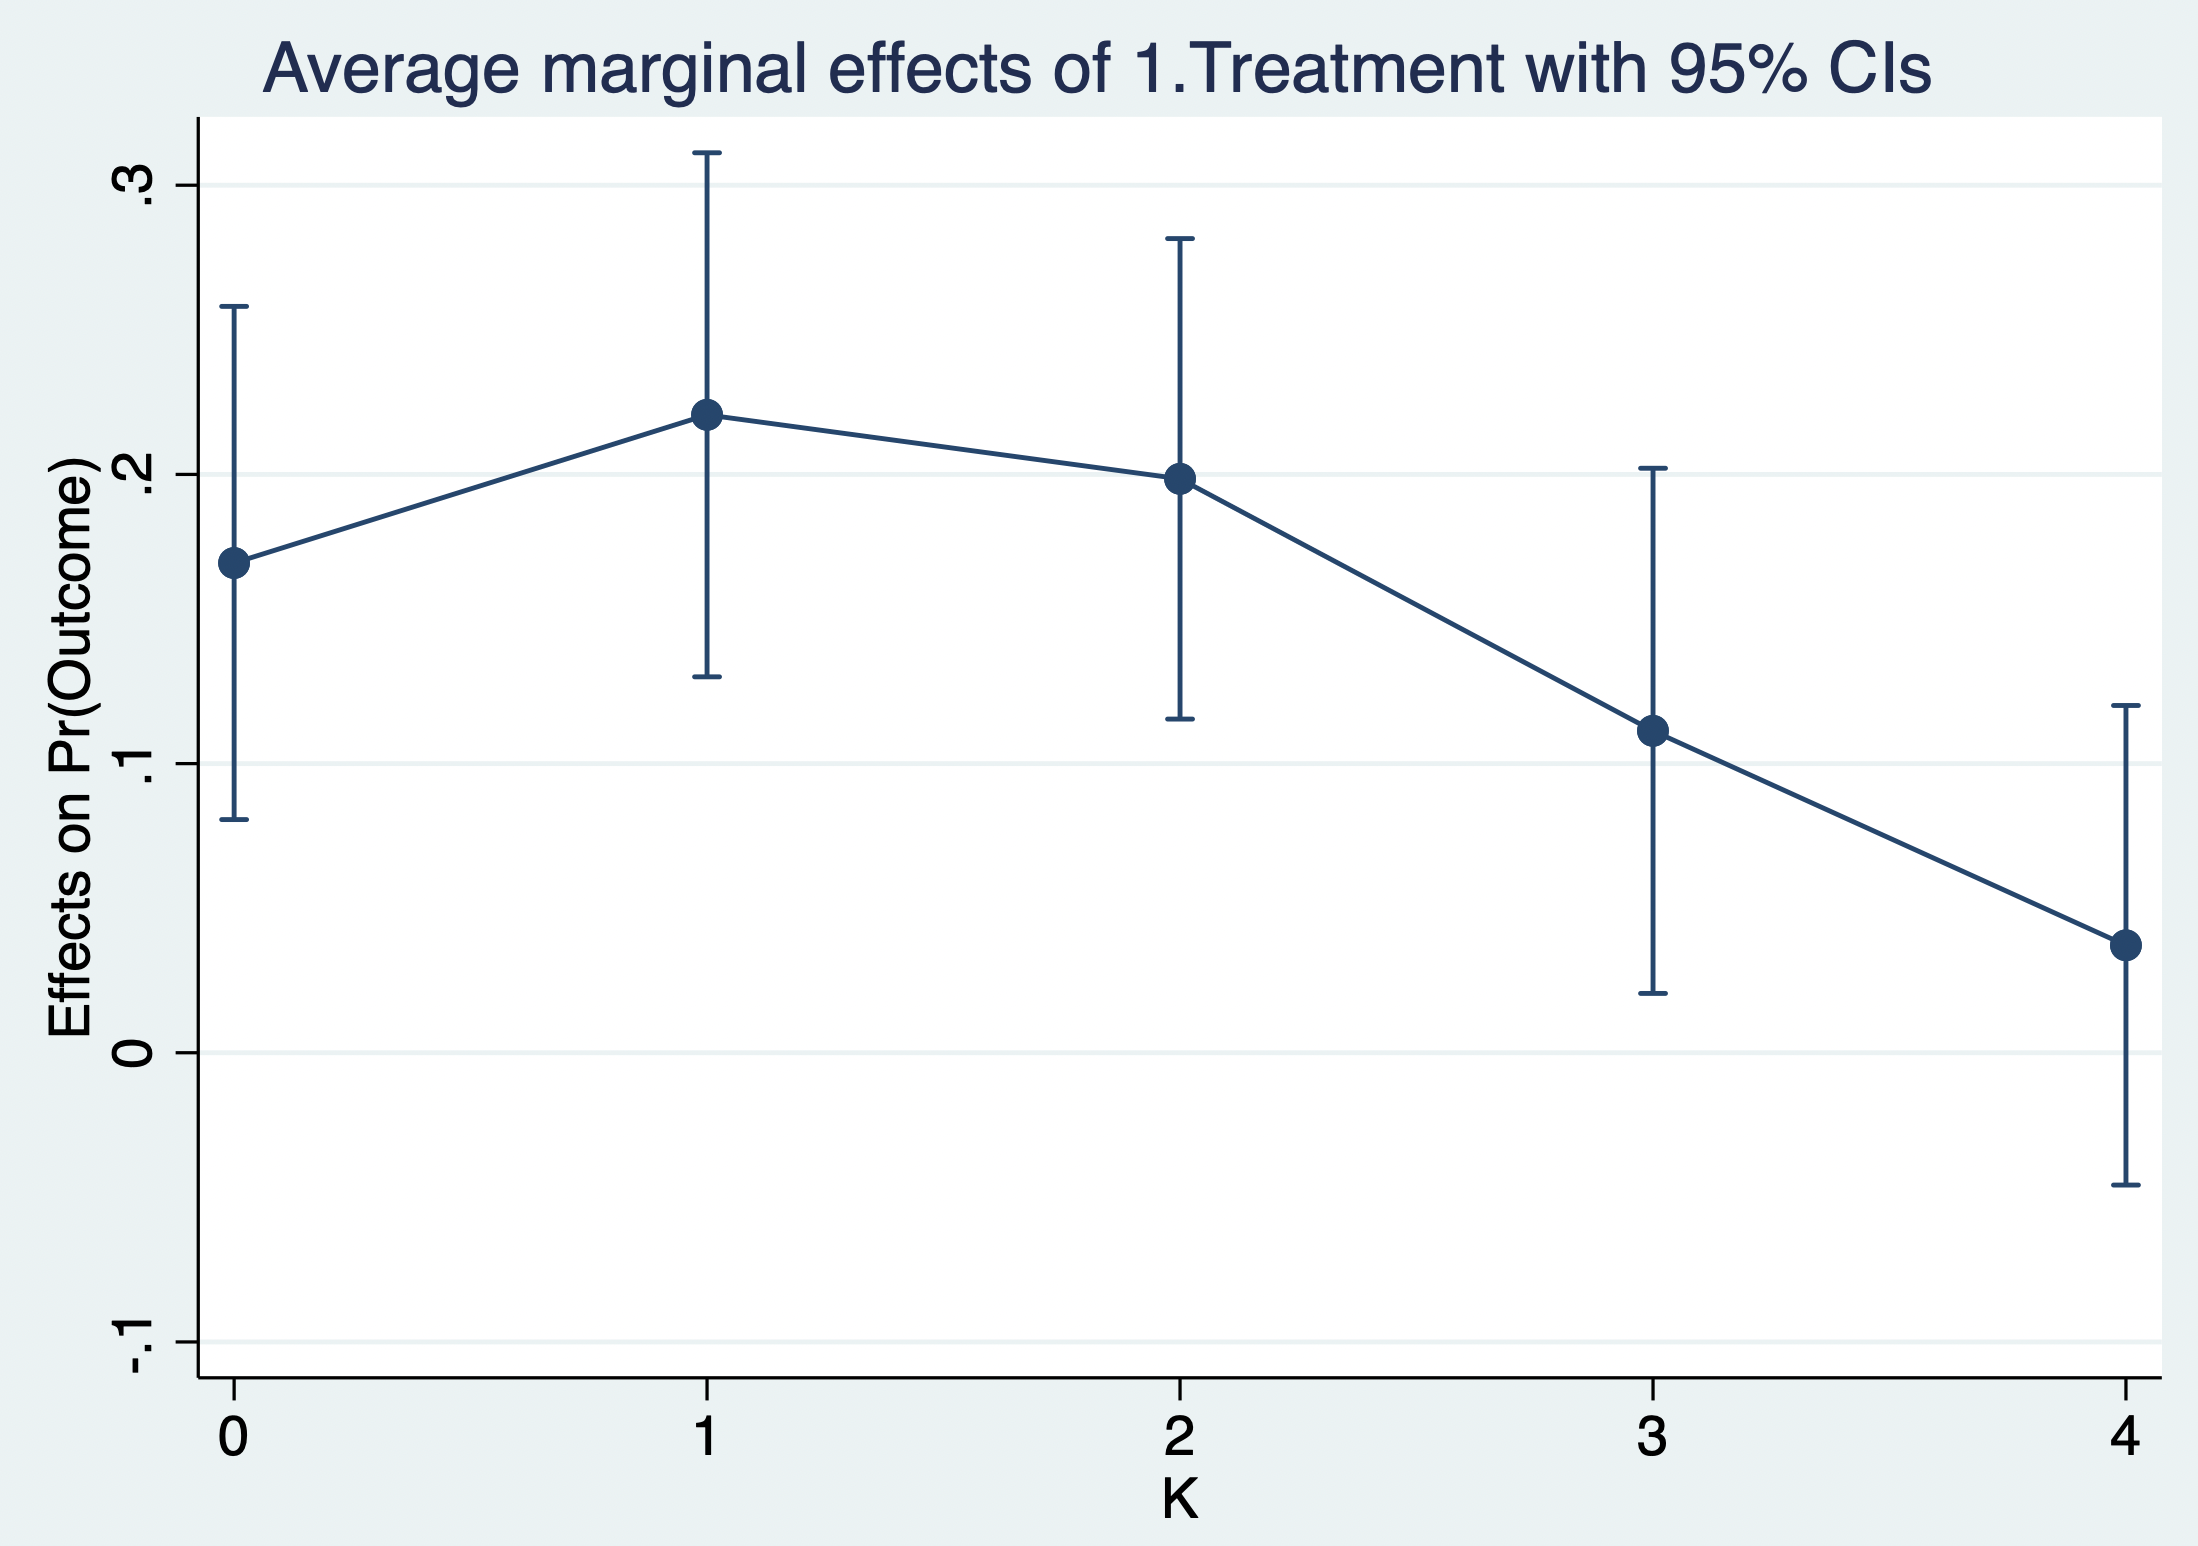
\includegraphics[width=5.76806in,height=\textheight,keepaspectratio]{chapters/images/ch9-image6.png}

\textbf{代码9.12输出内窥镜比显微镜缓解率的增加（纵轴）随侵袭性（横轴）变化}

上一节中50岁以下人群中的比值比为2.69，50岁以上人群中的比值比为1.59，直观上两者存在明显差异，因此年龄可能是手术方式对内分泌预后的修饰效应因子。同样采用交互项的方法统计检验年龄的修饰效应。虽然统计学检验未见年龄的修饰效应，但更直观的方法可以计算不同年龄段患者中的边际效应，可见随着年龄的增长，内窥镜组和显微镜组的差距越来越小。

\begin{tcolorbox}[enhanced jigsaw, arc=.35mm, bottomrule=.15mm, breakable, colback=white, colframe=quarto-callout-note-color-frame, left=2mm, leftrule=.75mm, opacityback=0, rightrule=.15mm, toprule=.15mm]

\vspace{-3mm}\textbf{代码9.13}\vspace{3mm}

\begin{Shaded}
\begin{Highlighting}[]
\KeywordTok{logit}\NormalTok{ Outcome i.Treatment }\KeywordTok{k}\NormalTok{ i.Treatment\#c.age age, }\KeywordTok{or}
\NormalTok{margins, }\KeywordTok{dydx}\NormalTok{(Treatment) }\FunctionTok{at}\NormalTok{(age=(15(5)80)) plot}
\end{Highlighting}
\end{Shaded}

\end{tcolorbox}

\begin{tcolorbox}[enhanced jigsaw, arc=.35mm, bottomrule=.15mm, breakable, colback=white, colframe=quarto-callout-note-color-frame, left=2mm, leftrule=.75mm, opacityback=0, rightrule=.15mm, toprule=.15mm]

\vspace{-3mm}\textbf{代码9.13输出}\vspace{3mm}

{\def\LTcaptype{none} % do not increment counter
\begin{longtable}[]{@{}
  >{\centering\arraybackslash}p{(\linewidth - 6\tabcolsep) * \real{0.4744}}
  >{\raggedright\arraybackslash}p{(\linewidth - 6\tabcolsep) * \real{0.1923}}
  >{\centering\arraybackslash}p{(\linewidth - 6\tabcolsep) * \real{0.1795}}
  >{\centering\arraybackslash}p{(\linewidth - 6\tabcolsep) * \real{0.1538}}@{}}
\toprule\noalign{}
\begin{minipage}[b]{\linewidth}\centering
Logistic regression
\end{minipage} & \begin{minipage}[b]{\linewidth}\raggedright
Number of obs
\end{minipage} & \begin{minipage}[b]{\linewidth}\centering
=
\end{minipage} & \begin{minipage}[b]{\linewidth}\centering
\textbf{743}
\end{minipage} \\
\midrule\noalign{}
\endhead
\bottomrule\noalign{}
\endlastfoot
& LR chi2(2) & = & \textbf{173.98} \\
\textbf{Log pseudolikelihood = -427.185} & Prob \textgreater{} chi2 & =
& \textbf{0.0000} \\
& Psudo R2 & = & \textbf{0.1692} \\
Outcome & Odds ratio & Std. err. & z \\
1.Treatment & \textbf{4.38435} & \textbf{2.812506} & \textbf{2.30} \\
k & \textbf{.4104892} & \textbf{.0336063} & \textbf{-10.88} \\
Treatment\#c.age 1 & \textbf{.9851654} & \textbf{.0137251} &
\textbf{-1.07} \\
age & \textbf{1.023341} & \textbf{.0101553} & \textbf{2.33} \\
\_cons & \textbf{1.239721} & \textbf{.5904421} & \textbf{0.45} \\
\end{longtable}
}

\end{tcolorbox}

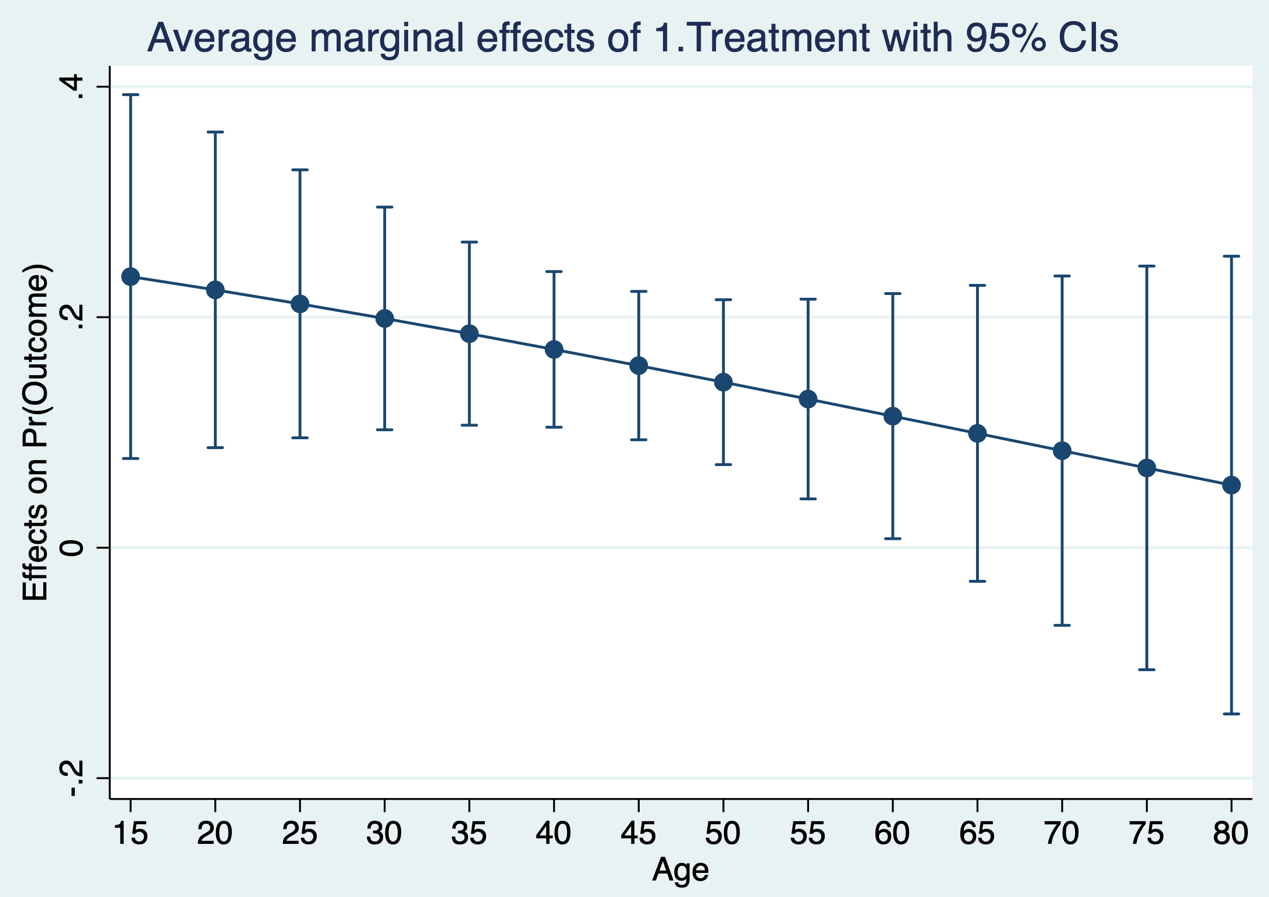
\includegraphics[width=5.76806in,height=\textheight,keepaspectratio]{chapters/images/ch9-image7.png}

\textbf{代码9.13输出内窥镜比显微镜缓解率的增加（纵轴）随年龄（横轴）变化}

\section{交互作用}\label{ux4ea4ux4e92ux4f5cux7528}

\begin{enumerate}
\def\labelenumi{\arabic{enumi}.}
\tightlist
\item
  反事实框架下的交互作用
\end{enumerate}

一般来说，如果同时给与个体两个或多个干预措施，观察到某个结果，我们将这两种或多种干预称为联合干预。两种治疗
T 和 T' 之间存在交互作用的定义为，如果将 T' 设为1的联合干预时 T 对 Y
的因果效应不同于将 T' 设置为 0 的联合干预时 T 对 Y 的因果效应。即

\textbf{公式 9.6　交互作用}

\[\Pr(Y^{T=1,T'=1}=1)-\Pr(Y^{T=0,T'=1}=1) \ne \Pr(Y^{T=1,T'=0}=1)-\Pr(Y^{T=0,T'=0}=1)\]

交互作用和修饰效应之间的区别在于修饰效应的概念着重 T 对 Y
的因果效应，而不是 V 对 Y
的因果效应。例如，年龄是手术效果的效应修饰因子，但从未提出年龄对手术效果的影响，并不认为年龄和手术方案是同等地位的变量，因为只有手术方案被认为是可以假设干预的变量。相反，交互作用的定义给予
T 和 T' 两种干预方法同等的地位，交互的概念指两种处理 T 和 T'
的联合因果效应。

换句话说，当治疗 T
是随机分配时，交互作用和修饰效应的计算方法是一致的，按照上一节中的方法替换效应修饰因子
V 为治疗
T'。非随机对照研究中，需要通过标准化或逆概率加权以矫正混杂因素，等效方法如下：可以将
T 和 T' 视为具有四个级别的组合干预（11, 01, 10, 00），而非将 T 和 T'
视为两种不同的干预。在这种情况下，交互作用的识别与传统的因果识别方法没有区别。

案例9.1交互作用

在案例9.1的数据中增加术者经验变量Surgeon，分为经验丰富（Experienced）和经验一般（Green）。两者以年手术量来划分。

\textbf{案例9.1交互作用数据表}

{\def\LTcaptype{none} % do not increment counter
\begin{longtable}[]{@{}cccccc@{}}
\toprule\noalign{}
ID & Surgeon & T & K & Y & LOS \\
\midrule\noalign{}
\endhead
\bottomrule\noalign{}
\endlastfoot
\ldots{} & \ldots{} & \ldots{} & \ldots{} & \ldots{} & \\
572 & Experienced & Endoscopy & 3 & No & 5 \\
573 & Green & Endoscopy & 0 & No & 8 \\
574 & Experienced & Endoscopy & 3 & Yes & 6 \\
575 & Experienced & Endoscopy & 3 & Yes & 6 \\
577 & Experienced & Microscopy & 2 & Yes & 5 \\
578 & Experienced & Microscopy & 0 & Yes & 6 \\
579 & Experienced & Microscopy & 3 & No & 9 \\
\ldots{} & \ldots{} & \ldots{} & \ldots{} & \ldots{} & \\
\end{longtable}
}

Treatment\_interact为新建的四个级别的组合干预：经验丰富的术者行内镜手术（1）；经验一般的术者行内镜手术（2）；经验丰富的术者行显微镜手术（3）；以及经验一般的术者行显微镜手术（4）。

\begin{tcolorbox}[enhanced jigsaw, arc=.35mm, bottomrule=.15mm, breakable, colback=white, colframe=quarto-callout-note-color-frame, left=2mm, leftrule=.75mm, opacityback=0, rightrule=.15mm, toprule=.15mm]

\vspace{-3mm}\textbf{代码9.14}\vspace{3mm}

\begin{Shaded}
\begin{Highlighting}[]
\KeywordTok{gen}\NormalTok{ Treatment1 = (surgeon == }\StringTok{"Experienced"}\NormalTok{)}
\KeywordTok{gen}\NormalTok{ Treatment\_interact = 1 }\KeywordTok{if}\NormalTok{ Treatment == 1 \& Treatment1 == 1}
\KeywordTok{replace}\NormalTok{ Treatment\_interact = 2 }\KeywordTok{if}\NormalTok{ Treatment == 1 \& Treatment1 == 0}
\KeywordTok{replace}\NormalTok{ Treatment\_interact = 3 }\KeywordTok{if}\NormalTok{ Treatment == 0 \& Treatment1 == 1}
\KeywordTok{replace}\NormalTok{ Treatment\_interact = 4 }\KeywordTok{if}\NormalTok{ Treatment == 0 \& Treatment1 == 0}
\KeywordTok{logit}\NormalTok{ Outcome i.Treatment\_interact }\KeywordTok{k}\NormalTok{, }\KeywordTok{or}
\end{Highlighting}
\end{Shaded}

\end{tcolorbox}

\begin{tcolorbox}[enhanced jigsaw, arc=.35mm, bottomrule=.15mm, breakable, colback=white, colframe=quarto-callout-note-color-frame, left=2mm, leftrule=.75mm, opacityback=0, rightrule=.15mm, toprule=.15mm]

\vspace{-3mm}\textbf{代码9.14输出}\vspace{3mm}

{\def\LTcaptype{none} % do not increment counter
\begin{longtable}[]{@{}
  >{\centering\arraybackslash}p{(\linewidth - 6\tabcolsep) * \real{0.4875}}
  >{\raggedright\arraybackslash}p{(\linewidth - 6\tabcolsep) * \real{0.1875}}
  >{\centering\arraybackslash}p{(\linewidth - 6\tabcolsep) * \real{0.1750}}
  >{\centering\arraybackslash}p{(\linewidth - 6\tabcolsep) * \real{0.1500}}@{}}
\toprule\noalign{}
\begin{minipage}[b]{\linewidth}\centering
Logistic regression
\end{minipage} & \begin{minipage}[b]{\linewidth}\raggedright
Number of obs
\end{minipage} & \begin{minipage}[b]{\linewidth}\centering
=
\end{minipage} & \begin{minipage}[b]{\linewidth}\centering
\textbf{743}
\end{minipage} \\
\midrule\noalign{}
\endhead
\bottomrule\noalign{}
\endlastfoot
& LR chi2(2) & = & \textbf{212.49} \\
\textbf{Log pseudolikelihood = -407.93941} & Prob \textgreater{} chi2 &
= & \textbf{0.0000} \\
& Psudo R2 & = & \textbf{0.2066} \\
Outcome & Odds ratio & Std. err. & z \\
Treatment\_interact & & & \\
2 & \textbf{.1472528} & \textbf{.0483119} & \textbf{-5.84} \\
3 & \textbf{.3145498} & \textbf{.063998} & \textbf{-5.68} \\
4 & \textbf{.1692625} & \textbf{.0505872} & \textbf{-5.94} \\
k & \textbf{.3966421} & \textbf{.0329938} & \textbf{-11.12} \\
\_cons & \textbf{13.09457} & \textbf{3.191546} & \textbf{10.55} \\
\end{longtable}
}

\end{tcolorbox}

经验丰富的术者行内镜手术（1）对比经验丰富的术者行显微镜手术（3）效果更好，结果比值比为0.315（p
= 0.000）。也可以经验一般的术者行内镜手术为参考进行比较。

\begin{tcolorbox}[enhanced jigsaw, arc=.35mm, bottomrule=.15mm, breakable, colback=white, colframe=quarto-callout-note-color-frame, left=2mm, leftrule=.75mm, opacityback=0, rightrule=.15mm, toprule=.15mm]

\vspace{-3mm}\textbf{代码9.15}\vspace{3mm}

\begin{Shaded}
\begin{Highlighting}[]
\KeywordTok{logit}\NormalTok{ Outcome ib(2).Treatment\_interact }\KeywordTok{k}\NormalTok{, }\KeywordTok{or}
\end{Highlighting}
\end{Shaded}

\end{tcolorbox}

\begin{tcolorbox}[enhanced jigsaw, arc=.35mm, bottomrule=.15mm, breakable, colback=white, colframe=quarto-callout-note-color-frame, left=2mm, leftrule=.75mm, opacityback=0, rightrule=.15mm, toprule=.15mm]

\vspace{-3mm}\textbf{代码9.15输出}\vspace{3mm}

{\def\LTcaptype{none} % do not increment counter
\begin{longtable}[]{@{}
  >{\centering\arraybackslash}p{(\linewidth - 6\tabcolsep) * \real{0.4875}}
  >{\raggedright\arraybackslash}p{(\linewidth - 6\tabcolsep) * \real{0.1875}}
  >{\centering\arraybackslash}p{(\linewidth - 6\tabcolsep) * \real{0.1750}}
  >{\centering\arraybackslash}p{(\linewidth - 6\tabcolsep) * \real{0.1500}}@{}}
\toprule\noalign{}
\begin{minipage}[b]{\linewidth}\centering
Logistic regression
\end{minipage} & \begin{minipage}[b]{\linewidth}\raggedright
Number of obs
\end{minipage} & \begin{minipage}[b]{\linewidth}\centering
=
\end{minipage} & \begin{minipage}[b]{\linewidth}\centering
\textbf{743}
\end{minipage} \\
\midrule\noalign{}
\endhead
\bottomrule\noalign{}
\endlastfoot
& LR chi2(2) & = & \textbf{212.49} \\
\textbf{Log pseudolikelihood = -407.93941} & Prob \textgreater{} chi2 &
= & \textbf{0.0000} \\
& Psudo R2 & = & \textbf{0.2066} \\
Outcome & Odds ratio & Std. err. & z \\
Treatment\_interact & & & \\
1 & \textbf{6.791041} & \textbf{2.228062} & \textbf{5.84} \\
3 & \textbf{2.136121} & \textbf{.6812429} & \textbf{2.38} \\
4 & \textbf{1.149468} & \textbf{.4432603} & \textbf{0.36} \\
k & \textbf{.3966421} & \textbf{.0329938} & \textbf{-11.12} \\
\_cons & \textbf{13.09457} & \textbf{3.191546} & \textbf{10.55} \\
\end{longtable}
}

\end{tcolorbox}

而经验一般的术者行内镜手术（2）对比经验一般的术者行显微镜手术（4）结果比值比为1.149（p

0.718），两者无明显差别。因此术者经验与手术方式存在交互作用，对于手术经验丰富的术者，内窥镜能显著提升缓解率；对于手术经验一般的术者，内窥镜和显微镜效果相当。

\begin{enumerate}
\def\labelenumi{\arabic{enumi}.}
\setcounter{enumi}{1}
\tightlist
\item
  充分病因框架下的交互作用
\end{enumerate}

再次考虑以上案例，有些患者只有接受内镜手术才能缓解，有些患者只有接受显微镜手术才能缓解，有些患者无论如何都不能缓解，有些患者无论如何都能缓解。这表明手术治疗并不是唯一决定预后的变量。流行病学中的充分病因模型可以用于解释交互作用，充分病因是指导致疾病发生的最少条件的干预组合，也就是说充分病因中的因素中都是导致疾病所必需的。举一个简单的例子，假设接受内镜手术且肿瘤较小的患者都缓解了，称内窥镜干预（T
= 1）和肿瘤大小（U1 =
0）是结果（缓解）的充分病因。另假设接受显微镜手术且肿瘤呈侵袭性的都没有缓解，称干预（T
= 0）和肿瘤侵袭性（U2 =
1）是结果（未缓解）的充分病因。同理，可以将充分病因的描述推广至两种治疗的交互作用中。

T 和 T' 之间存在充分病因交互作用，如果同时给予 T 和 T'
能产生某个结局。如假设个体由经验丰富的术者行内镜手术时能缓解，但在其他情况下都无法缓解，则术者经验和手术方式存在充分病因交互作用。充分病因交互作用可以是协同的或拮抗的。在充分-组分病因框架下识别协同（synergism）的形式化条件，可参见
VanderWeele 与 Robins（2007）。

协同作用：当两个或两个以上因子共同作用时，其效应明显大于这些因子单独作用时的和或积，称之为协同作用，也称正交互。

拮抗作用：当两个或两个以上因子共同作用时，其效应明显小于这些因子单独作用时的和或积，称之为拮抗作用，也称负交互。

\begin{enumerate}
\def\labelenumi{\arabic{enumi}.}
\setcounter{enumi}{2}
\tightlist
\item
  结合反事实和充分病因框架下的交互作用
\end{enumerate}

结合反事实框架以及充分病因框架对交互作用的类型进行分类，可阐明交互的含义。考虑案例9.1交互作用，可以推断出缓解的9种原因。

\begin{enumerate}
\def\labelenumi{\arabic{enumi})}
\item
  内镜手术（与术者经验无关）
\item
  显微镜手术（与术者经验无关）
\item
  经验丰富的术者（与手术方式无关）
\item
  经验一般的术者（与手术方式无关）
\item
  经验丰富的术者行内镜手术
\item
  经验一般的术者行内镜手术
\item
  经验丰富的术者行显微镜手术
\item
  经验一般的术者行显微镜手术
\item
  通过其他机制（与术者经验和手术方式均无关）
\end{enumerate}

通过计算不同原因的边际值，表示这 9
个充分病因的因果饼图（图9.4），红色百分比代表各种原因下的边际缓解概率。

\begin{tcolorbox}[enhanced jigsaw, arc=.35mm, bottomrule=.15mm, breakable, colback=white, colframe=quarto-callout-note-color-frame, left=2mm, leftrule=.75mm, opacityback=0, rightrule=.15mm, toprule=.15mm]

\vspace{-3mm}\textbf{代码9.16}\vspace{3mm}

\begin{Shaded}
\begin{Highlighting}[]
\KeywordTok{gen}\NormalTok{ surg\_exp = (surgeon == }\StringTok{"Experienced"}\NormalTok{)}
\KeywordTok{logit}\NormalTok{ Outcome i.Treatment i.surg\_exp }\KeywordTok{k}\NormalTok{ age i.Treatment\#i.surg\_exp, }\KeywordTok{or}
\NormalTok{margins i.Treatment i.surg\_exp i.Treatment\#i.surg\_exp}
\end{Highlighting}
\end{Shaded}

\end{tcolorbox}

\begin{tcolorbox}[enhanced jigsaw, arc=.35mm, bottomrule=.15mm, breakable, colback=white, colframe=quarto-callout-note-color-frame, left=2mm, leftrule=.75mm, opacityback=0, rightrule=.15mm, toprule=.15mm]

\vspace{-3mm}\textbf{代码9.16输出}\vspace{3mm}

{\def\LTcaptype{none} % do not increment counter
\begin{longtable}[]{@{}llc@{}}
\toprule\noalign{}
Average marginal effects & Number of obs = & \textbf{743} \\
\midrule\noalign{}
\endhead
\bottomrule\noalign{}
\endlastfoot
Model VCE: OIM & & \\
& & \\
Expression: Pr(Outcome), predict() & & \\
& Delta-method & \\
Margin & Std. err. & z \\
Treatment & & \\
0 & \textbf{.4036051} & \textbf{.0213112} \\
1 & \textbf{.5625797} & \textbf{.0224486} \\
surg\_exp & & \\
0 & \textbf{.3030656} & \textbf{.0321055} \\
1 & \textbf{.5303804} & \textbf{.0185119} \\
Treatment\#surg\_exp & & \\
0 0 & \textbf{.3151536} & \textbf{.0434869} \\
0 1 & \textbf{.4291778} & \textbf{.0246149} \\
1 0 & \textbf{.2864942} & \textbf{.0482572} \\
1 1 & \textbf{.6460793} & \textbf{.026193} \\
\end{longtable}
}

\end{tcolorbox}

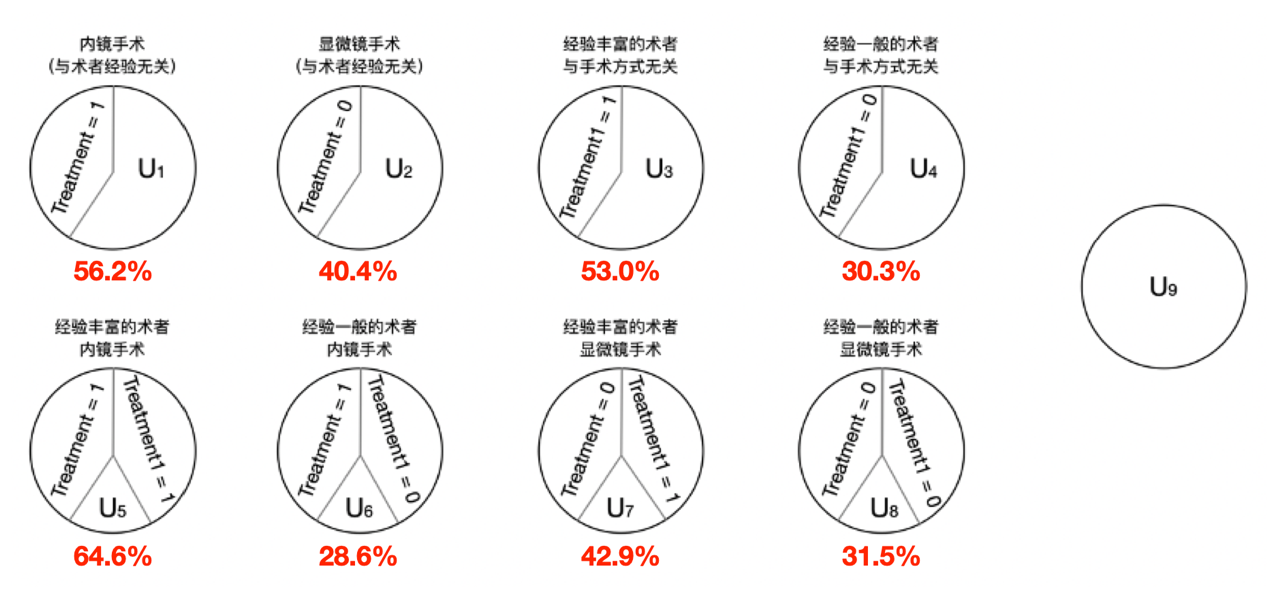
\includegraphics[width=5.76806in,height=\textheight,keepaspectratio]{chapters/images/ch9-image8.png}

\textbf{图9.4反事实与充分病因框架下的交互作用}

参考文献：

1.~Hernán~MA, Robins JM (2020). Causal Inference: What If. Boca Raton:
Chapman \& Hall/CRC.

2. Zhang J, Yu KF. What's the relative risk? A method of correcting the
odds ratio in cohort studies of common outcomes. JAMA, 1998,
280(19):1690-1691.

3. Schisterman EF, Cole SR, Platt RW. Overadjustment bias and
unnecessary adjustment in epidemiologic studies. Epidemiology, 2009,
20(4):488-495.

4. VanderWeele TJ. On the distinction between interaction and effect
modification. Epidemiology, 2009, 20(6):863-871.

5. VanderWeele TJ, Robins JM. The identification of synergism in the
sufficient-component-cause framework. Epidemiology, 2007, 18(3):329-339.

\bookmarksetup{startatroot}

\chapter{基于倾向评分的因果推断方法}\label{ux57faux4e8eux503eux5411ux8bc4ux5206ux7684ux56e0ux679cux63a8ux65adux65b9ux6cd5}

在因果推断中，对于某个接受干预的个体，在对照组中找到与其各方面特征都一致的个体将其配对。对干预组中的其他个体采取同样的操作，在对照组中寻找相似的个体进行两两配对。如果能保证配对的两个组中个体的完全相似，那就可以在配对的个体中直接计算因果效应。简而言之，配对就是寻找对照组与干预组中相似的个体，在配对的个体中估计因果效应。配对过程大致上可以分为四个步骤：定义相似性，实施配对，检验配对效果，估计因果效应。配对优于回归之处在于：配对的时候研究者没有任何结局变量的信息，只有在完成配对以后才会用到结局变量，这样就保证了研究的科学性，避免了回归中的主观因素（即为了得到有意义的p值对纳入的控制变量反复多次调整）。这种``先设计、后分析''的做法有助于减少因查看结局后反复调整模型带来的主观性；但配对并不天然优于回归，仍须依赖协变量测量充分、模型设定合理和匹配后平衡可接受等条件。

利用协变量（x1，x2，\ldots\ldots，xk）进行配对，一般使用标准化欧式距离来测量两个样本之间的相似性。

\[d(x_i,x_j)=\sqrt{\sum_{k=1}^{K}\frac{(x_{ki}-x_{kj})^2}{\sigma_k^2}}\]

表示两个样本 和 之间的距离，
是某个变量的标准差。那么以样本的哪些特征来测量他们的距离呢？临床研究中样本的特征常常是多个维度的，包括年龄、性别、疾病严重程度、治疗史等等。维度太多带来了计算的复杂性，因此，如果能找到一个简单的变量，用于衡量样本与样本之间的距离，就能大大简化计算。

\section{倾向性评分（Propensity
Score）}\label{ux503eux5411ux6027ux8bc4ux5206propensity-score}

倾向性评分的含义是指接受某种干预的概率。在1:1分配的随机对照研究，每个个体接受该干预的概率都为50\%，因此，每个个体的倾向性评分即为0.5，而非随机对照研究当中的倾向性评分需要去估计。估计的方程在考虑所有混杂因素的情况下接受某种干预的概率，即更严格地说，倾向评分是在给定处理前协变量
X 后接受处理的条件概率
e(X)=Pr(A=1\textbar X)；它用于构造协变量分布可比的样本或加权伪总体，而不是直接估计因果效应。

\[PS(x_i)=Pr[A=1\mid x_i]\]

是这个样本的混杂因素。

倾向性评分的估计一般采用回归方程，将干预变量对所有的混杂因素进行回归。然后得出干预的预测概率即为该干预的倾向性评分。也可以运用一些机器学习的方法来进行倾向性评分的估计。建模的首要目标不是提高对处理分配的预测准确性，而是使后续匹配或加权后的基线协变量达到平衡。协变量应在处理发生前测量，并结合临床知识与因果图选取；不应按单变量
P 值筛选，也不应纳入处理后的变量或碰撞因子。

采用案例9.1的数据，估计接受内窥镜手术的概率，并显示倾向性评分的分布。红色区域为干预组，即为内窥镜组，蓝色区域为对照组，即显微镜组。红色组和蓝色组的倾向性评分都基本分布在0.3到0.6之间，两组的重叠性较高。

\begin{tcolorbox}[enhanced jigsaw, arc=.35mm, bottomrule=.15mm, breakable, colback=white, colframe=quarto-callout-note-color-frame, left=2mm, leftrule=.75mm, opacityback=0, rightrule=.15mm, toprule=.15mm]

\vspace{-3mm}\textbf{代码10.1}\vspace{3mm}

\begin{Shaded}
\begin{Highlighting}[]
\NormalTok{. psmatch2 Treatment }\KeywordTok{k}\NormalTok{ age, }\KeywordTok{logit}
\NormalTok{. psgraph, }\BaseNTok{bin}\NormalTok{(40)}
\end{Highlighting}
\end{Shaded}

\end{tcolorbox}

\begin{tcolorbox}[enhanced jigsaw, arc=.35mm, bottomrule=.15mm, breakable, colback=white, colframe=quarto-callout-note-color-frame, left=2mm, leftrule=.75mm, opacityback=0, rightrule=.15mm, toprule=.15mm]

\vspace{-3mm}\textbf{代码10.1输出}\vspace{3mm}

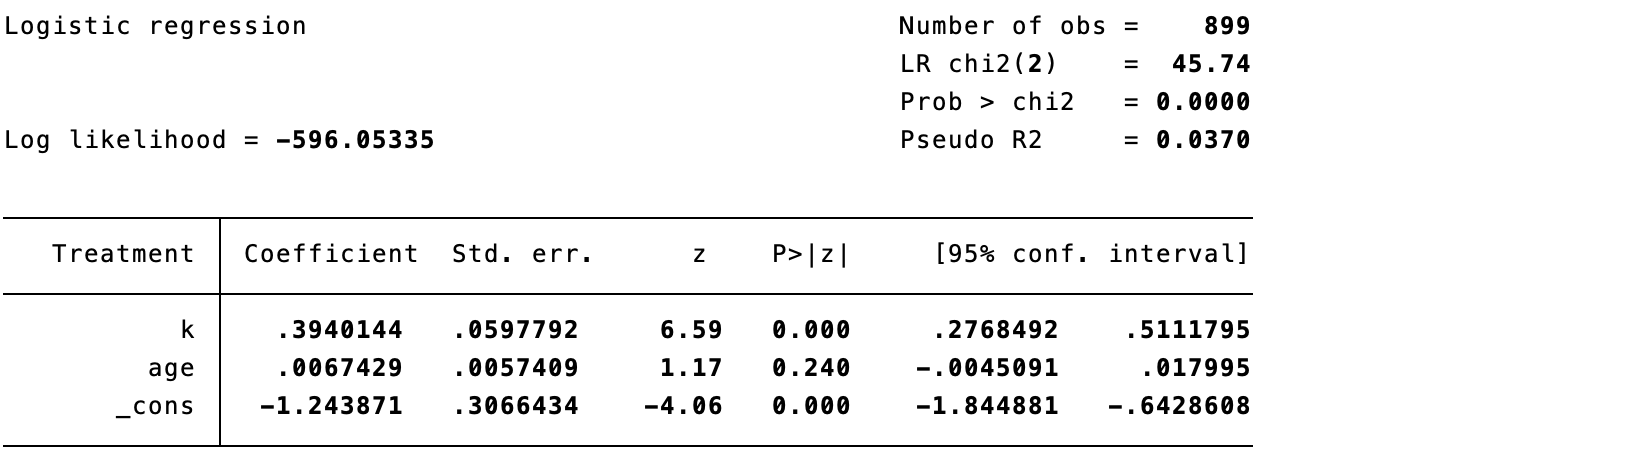
\includegraphics[width=1\linewidth,height=\textheight,keepaspectratio]{chapters/images/ch10-image1.png}

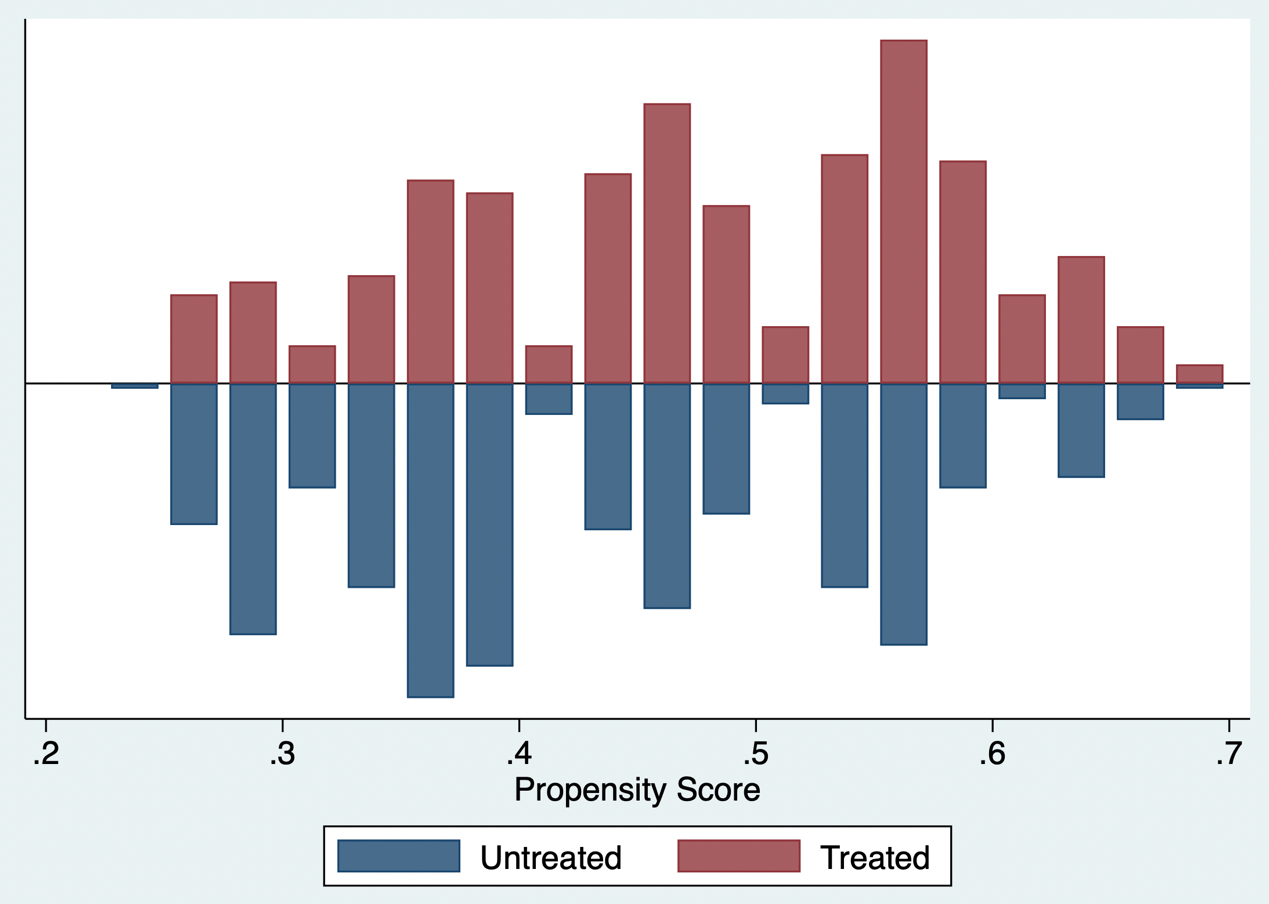
\includegraphics[width=0.85\linewidth,height=\textheight,keepaspectratio]{chapters/images/ch10-image2.png}

\end{tcolorbox}

倾向性评分提示肿瘤侵袭性越高（k），患者接受内窥镜治疗的概率越高。

与之前讨论过的所有因果推断方法一样，使用倾向性评分法需要具备可交换性、重叠性和一致性等识别条件。如果阻断混杂因素后可消除后门路径，那么阻断PS
也可消除后门路径。因此，在协变量水平内，干预组与对照组的可交换性意味着倾向性评分水平内的可交换性。此外，利用倾向性评分来进行因果推断的一个重要的前提是需要考虑倾向性得分的重叠性。图10.1中左边的曲线中，灰色的区域两条曲线有相当一部分的受试者重合，然而在右边的曲线中，两组人群区分的比较开，两者之间的重叠性较差。因此在右边的数据中进行因果推断就比较困难。当然，倾向性评分只平衡了测量的协变量，这并不能防止未测量因素的残留混杂。随机化同时平衡了测量的和未测量的协变量，因此它是消除混杂的首选方法。因此，实施匹配或加权前后均应检查倾向评分的分布与各基线协变量的平衡；倾向评分重叠本身不能替代协变量平衡诊断。

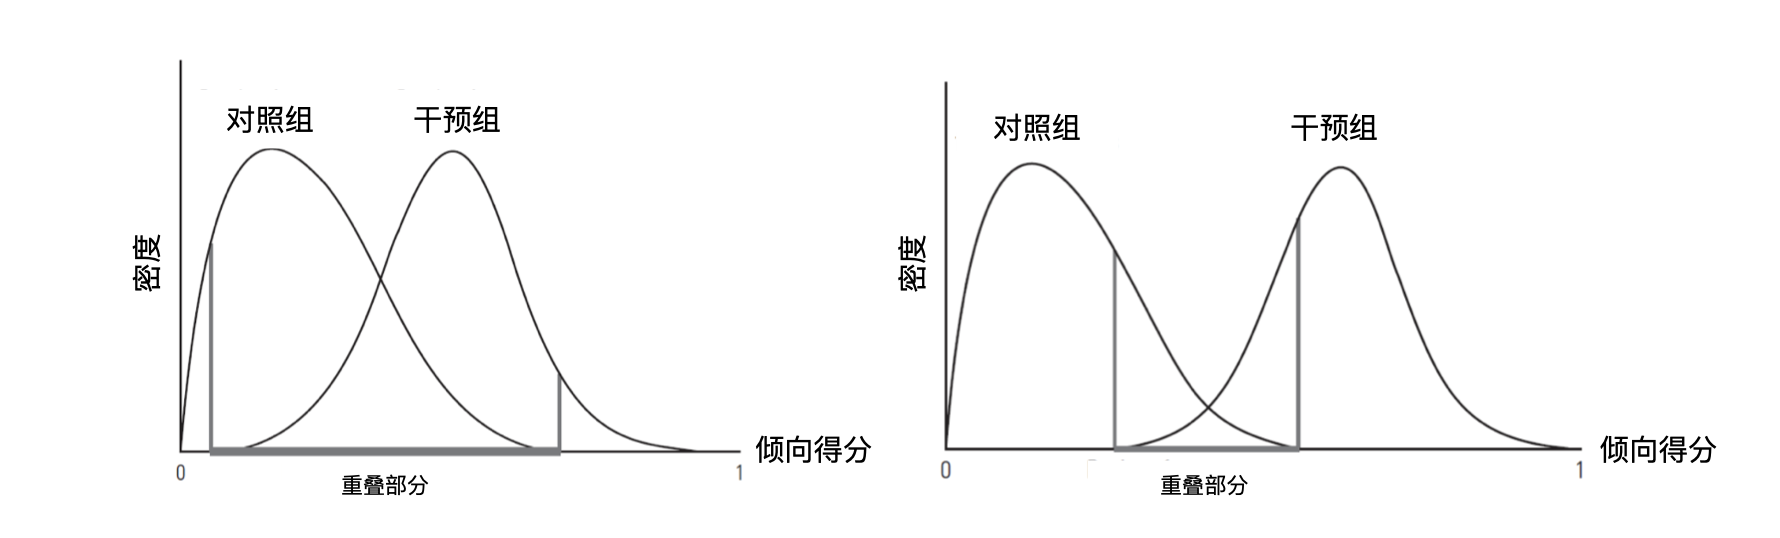
\includegraphics[width=1\linewidth,height=\textheight,keepaspectratio]{chapters/images/ch10-image3.png}

\textbf{图10.1 重叠性较好与较差的倾向性评分}

利用倾向性评分来进行因果推断有三种方法。

\section{直接将倾向评分加入到回归方程}\label{ux76f4ux63a5ux5c06ux503eux5411ux8bc4ux5206ux52a0ux5165ux5230ux56deux5f52ux65b9ux7a0b}

作为回归方程中的唯一协变量

\begin{tcolorbox}[enhanced jigsaw, arc=.35mm, bottomrule=.15mm, breakable, colback=white, colframe=quarto-callout-note-color-frame, left=2mm, leftrule=.75mm, opacityback=0, rightrule=.15mm, toprule=.15mm]

\vspace{-3mm}\textbf{代码10.2}\vspace{3mm}

\begin{Shaded}
\begin{Highlighting}[]
\NormalTok{. }\KeywordTok{reg}\NormalTok{ Outcome Treatment \_pscore, }\KeywordTok{or}
\end{Highlighting}
\end{Shaded}

\end{tcolorbox}

\begin{tcolorbox}[enhanced jigsaw, arc=.35mm, bottomrule=.15mm, breakable, colback=white, colframe=quarto-callout-note-color-frame, left=2mm, leftrule=.75mm, opacityback=0, rightrule=.15mm, toprule=.15mm]

\vspace{-3mm}\textbf{代码10.2输出}\vspace{3mm}

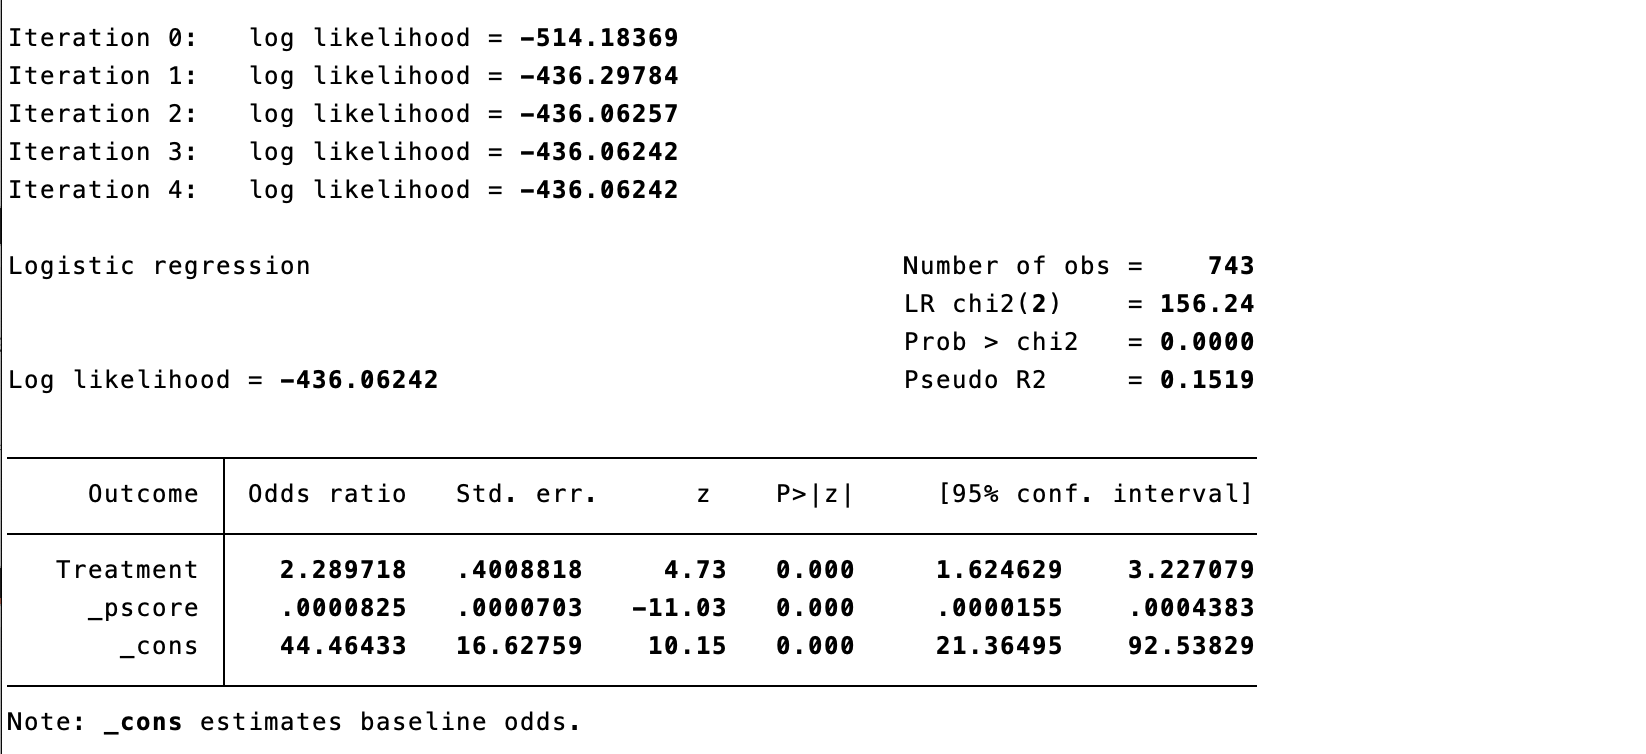
\includegraphics[width=1\linewidth,height=\textheight,keepaspectratio]{chapters/images/ch10-image4.png}

\end{tcolorbox}

回归结果提示内窥镜组显著增加内分泌缓解率，比值比为2.29，95\%置信区间为1.62-3.22，p值0.000。此处报告的
OR
属于条件效应，未必等同于边际风险比或风险差；为便于临床解释，宜同时给出标准化后的绝对风险、风险差或风险比及其
95\% 置信区间。

\section{利用倾向性评分进行匹配}\label{ux5229ux7528ux503eux5411ux6027ux8bc4ux5206ux8fdbux884cux5339ux914d}

将倾向评分相同的干预组和对照组之间进行配对，在配对的新样本当中进行因果推断。利用倾向评分进行匹配的原理如图10.2所示，黑色小人代表干预组，黄色小人代表对照组。其倾向性评分在x轴上表示，靠近0代表被分配到干预组的概率很小，靠近1代表分配到干预组的概率较大。倾向性评分匹配第一步从干预组中抽取一个个体，计算其倾向性评分，在对照组中寻找倾向性评分与其最近的黄色小人，将这两个小人形成一个配对。利用同样的方法重复操作，反复进行配对。最后在匹配好的样本中进行因果效应估计。此过程可能会剩下一些没有匹配到的患者，比如说靠近倾向性评分为0附近的黄色小人没有匹配到。

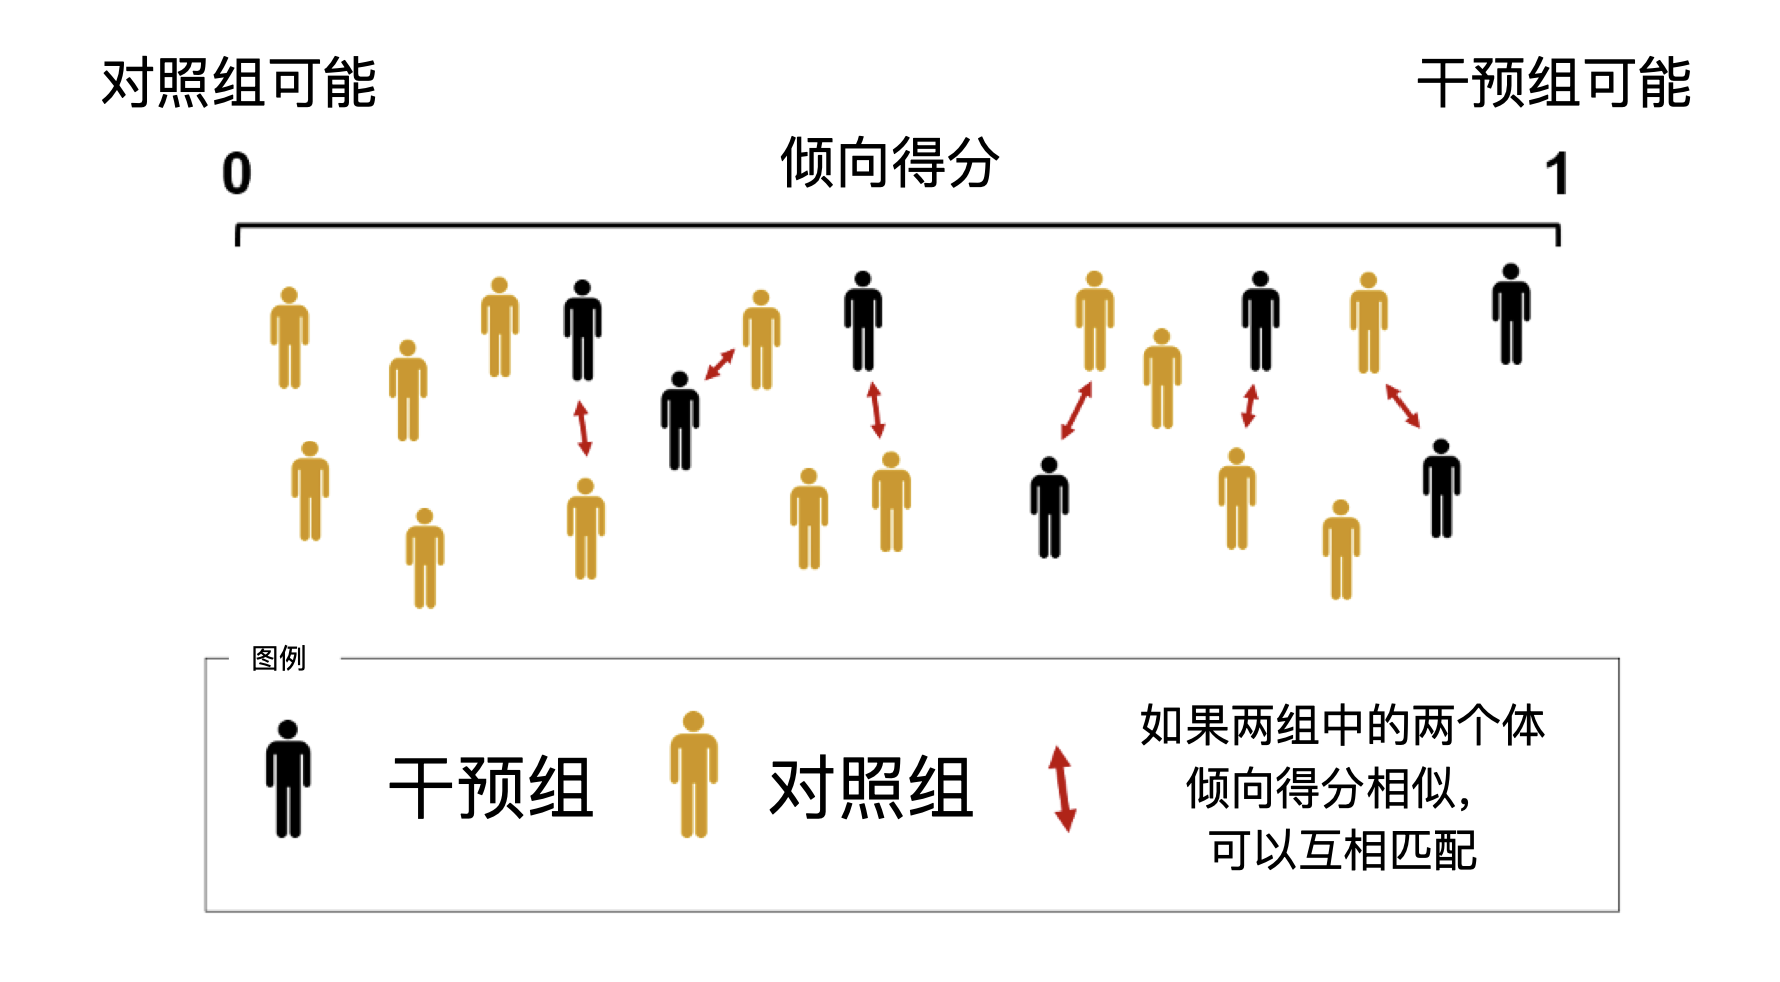
\includegraphics[width=1\linewidth,height=\textheight,keepaspectratio]{chapters/images/ch10-image5.png}

\textbf{图10.2 倾向性评分匹配原理}

实际的配对操作中可能会遇到四个问题：

一对一或一对多配对：一对一即干预组中的样本在对照组中寻找一个距离最近的样本与其匹配。一对多即干预组中的样本在对照组中寻找多个距离最近的样本与其匹配。一般而言，一对一匹配样本相似性比较好，但可能导致匹配后的样本量不足；而一对多匹配样本相似性没有较好满足，但匹配后的样本量充足。实际情况中，如果原始数据中对照组的样本量与干预组差距很大，可以选择一对多匹配。

如何定义距离最近？定义卡尺（caliper），允许两个样本进行匹配的最大距离。可以想象一下两个样本距离多近才能够匹配，如果卡尺太小，就会导致许多样本无法得到匹配，如卡尺定为0.001，即两样本相差0.001距离才能被匹配，就可能导致许多样本无法匹配。卡尺定太大，就会导致许多样本距离很大，也会被匹配到，可交换性得不到满足。实务中常以
logit(PS) 标准差的 0.2 作为 1:1
最近邻匹配的起始卡尺，并需结合匹配后协变量平衡、样本损失与临床可比性调整，而不应机械套用单一数值。

对照组中的个体是否可以重复匹配？如果原始数据中对照组的样本量远远小于治疗组，为了不损失治疗组的样本量，可以重复匹配对照组。

如果对照组中有多个样本与需要匹配的干预组样本距离一致如何操作？一对一匹配的前提下可以随机选择其中一个，也可以全部纳入，指定每个样本的权重，计算多个样本的加权平均值。

\begin{tcolorbox}[enhanced jigsaw, arc=.35mm, bottomrule=.15mm, breakable, colback=white, colframe=quarto-callout-note-color-frame, left=2mm, leftrule=.75mm, opacityback=0, rightrule=.15mm, toprule=.15mm]

\vspace{-3mm}\textbf{代码10.3}\vspace{3mm}

\begin{Shaded}
\begin{Highlighting}[]
\NormalTok{. psmatch2 Treatment }\KeywordTok{k}\NormalTok{ age, }\KeywordTok{logit}\NormalTok{ outcome(Outcome) n(1) cal(0.01) ties}
\end{Highlighting}
\end{Shaded}

\end{tcolorbox}

\begin{tcolorbox}[enhanced jigsaw, arc=.35mm, bottomrule=.15mm, breakable, colback=white, colframe=quarto-callout-note-color-frame, left=2mm, leftrule=.75mm, opacityback=0, rightrule=.15mm, toprule=.15mm]

\vspace{-3mm}\textbf{代码10.3输出}\vspace{3mm}

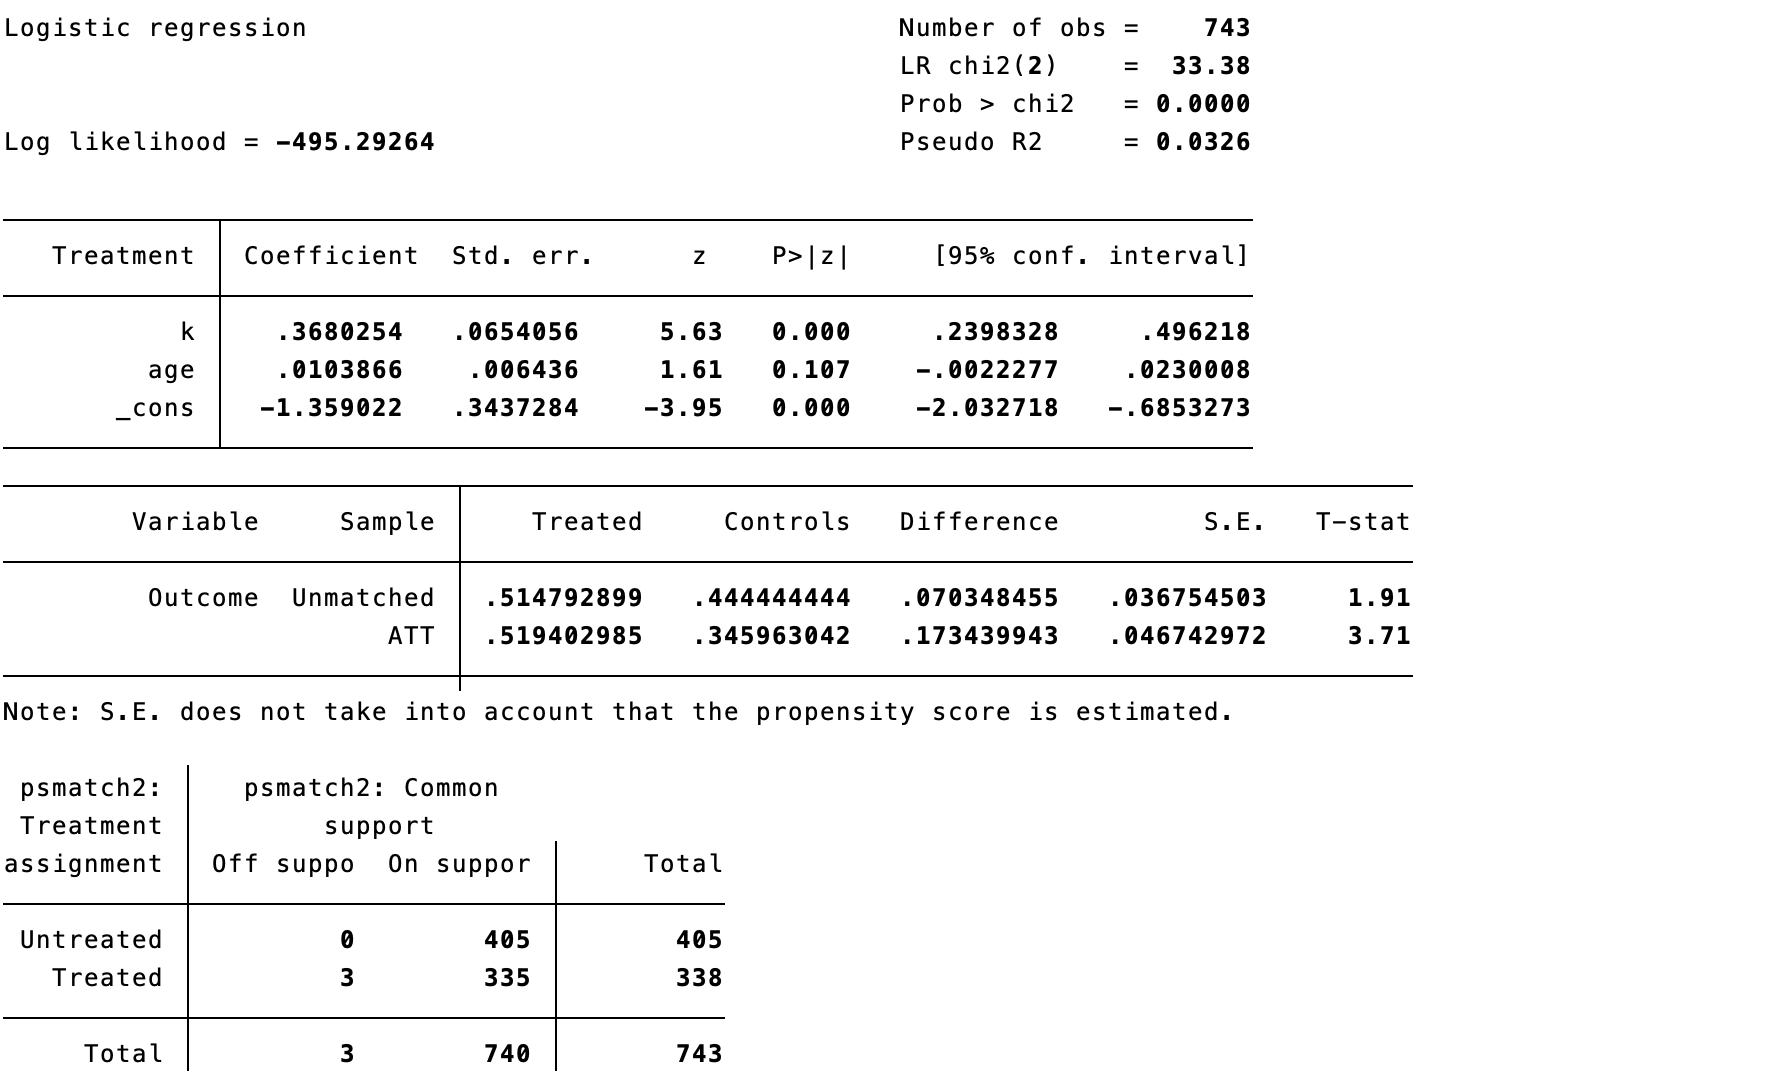
\includegraphics[width=1\linewidth,height=\textheight,keepaspectratio]{chapters/images/ch10-image6.png}

\end{tcolorbox}

\begin{tcolorbox}[enhanced jigsaw, arc=.35mm, bottomrule=.15mm, breakable, colback=white, colframe=quarto-callout-note-color-frame, left=2mm, leftrule=.75mm, opacityback=0, rightrule=.15mm, toprule=.15mm]

\vspace{-3mm}\textbf{代码10.4}\vspace{3mm}

\begin{Shaded}
\begin{Highlighting}[]
\NormalTok{. psmatch2 Treatment }\KeywordTok{k}\NormalTok{ age, }\KeywordTok{logit}\NormalTok{ outcome(Outcome) n(1) cal(0.001) ties}
\end{Highlighting}
\end{Shaded}

\end{tcolorbox}

\begin{tcolorbox}[enhanced jigsaw, arc=.35mm, bottomrule=.15mm, breakable, colback=white, colframe=quarto-callout-note-color-frame, left=2mm, leftrule=.75mm, opacityback=0, rightrule=.15mm, toprule=.15mm]

\vspace{-3mm}\textbf{代码10.4输出}\vspace{3mm}

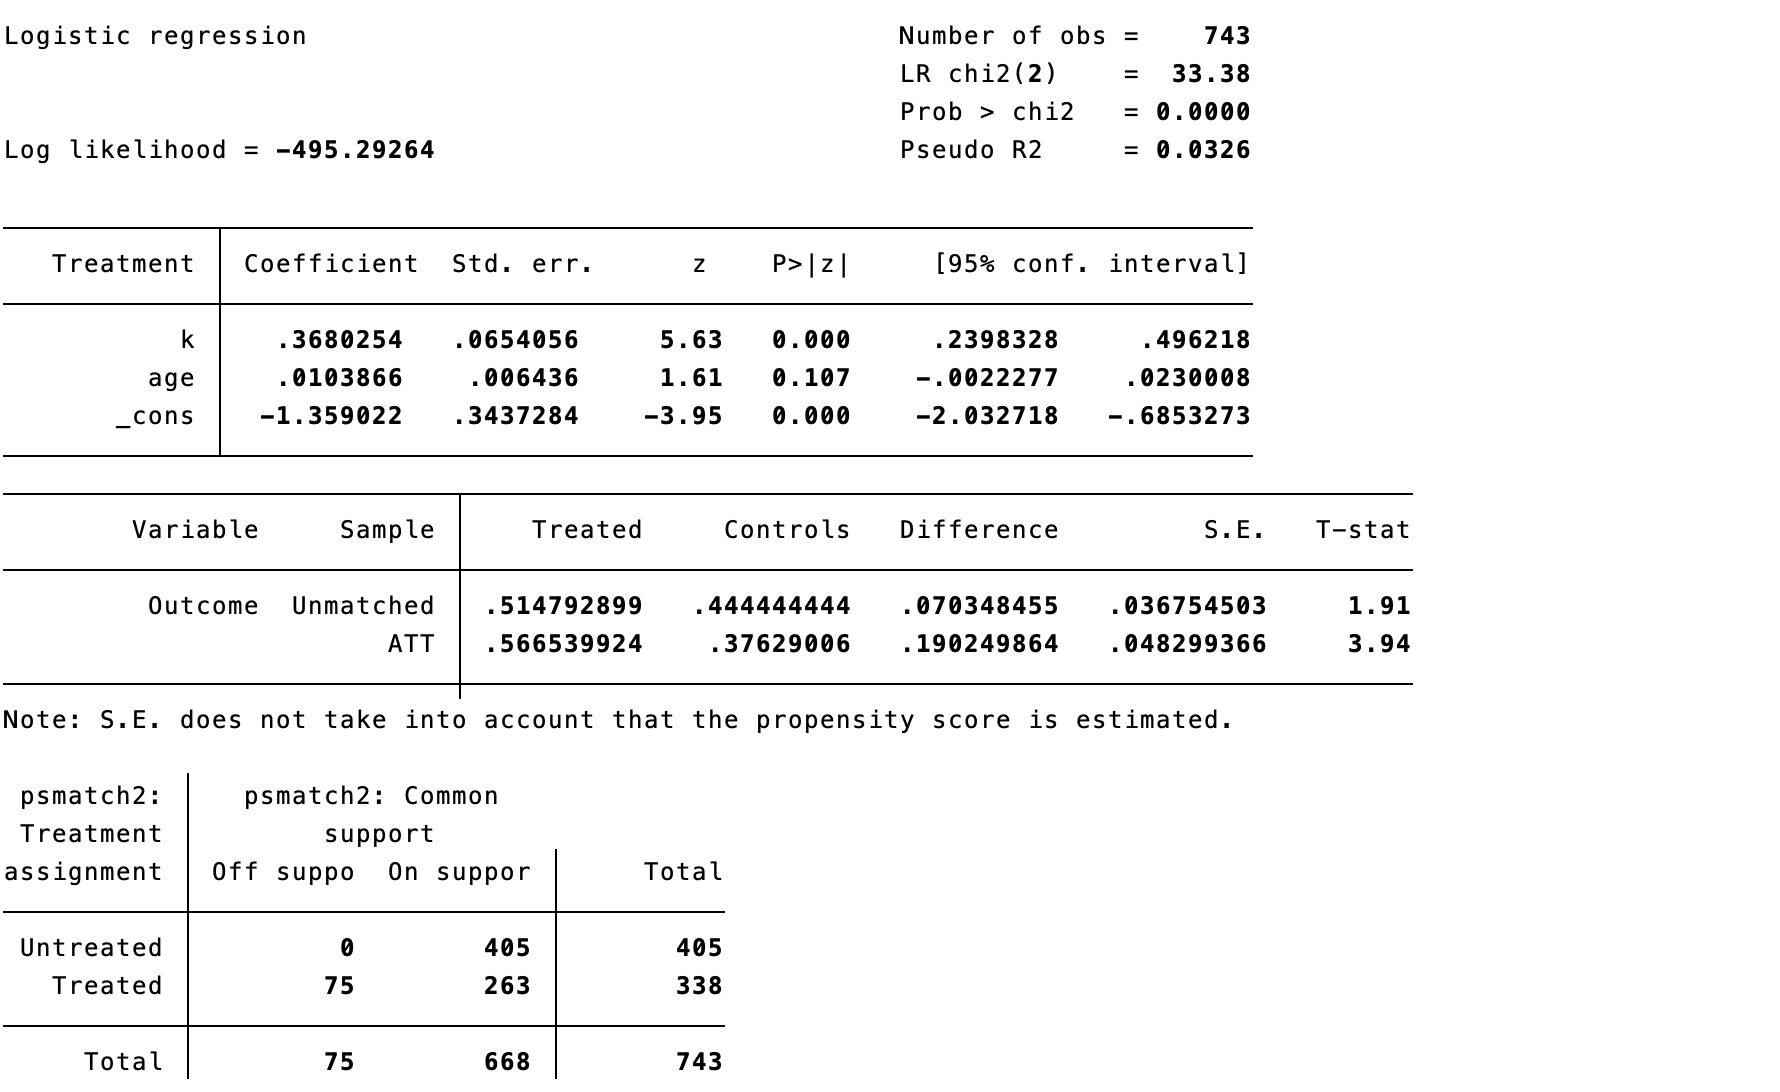
\includegraphics[width=1\linewidth,height=\textheight,keepaspectratio]{chapters/images/ch10-image7.png}

\end{tcolorbox}

卡尺定为0.01时只有3例患者无法匹配，而卡尺定为0.001时有75例无法匹配。需要指出的是匹配后的纳入样本往往和原始数据中的样本不同，因此基于匹配方法得到的因果效应估计也是针对匹配后的样本，称为干预组中的因果效应（Average
treatment effect in the
treated，ATT）。干预组中的缓解率为56.7\%，对照组中的缓解率为37.6\%，计算比值比为2.17。匹配会改变分析人群，故应明确此处估计的目标人群（通常为可匹配治疗者的
ATT），并报告未匹配者的数量与基线特征。

配对分析后的检验如同随机对照临床研究一样需要给出配对后的干预组和对照组各个变量的分布情况，查看是否有变量存在不平衡。下表为输出，U
代表没有匹配的样本，M
代表匹配样本。侵袭度在没有匹配当的样本中，干预组是2.2，对照组为1.7，
t检验的p值是0.000，代表两组之间有明显差别的。而在匹配的样本中干预组和对照组都为2.1，t检验的p值是1.000。匹配后的样本中，把侵袭性这样一个不均衡的指标给均衡了。同样倾向性评分方程中所有的指标在匹配以的样本中都均衡了。平衡诊断建议以每个协变量的绝对标准化均数差（absolute
SMD）为主，常以 \textless0.10 作为经验阈值；不应以 t 检验 P
值是否显著作为是否平衡的判据。

\begin{tcolorbox}[enhanced jigsaw, arc=.35mm, bottomrule=.15mm, breakable, colback=white, colframe=quarto-callout-note-color-frame, left=2mm, leftrule=.75mm, opacityback=0, rightrule=.15mm, toprule=.15mm]

\vspace{-3mm}\textbf{代码10.5}\vspace{3mm}

\begin{Shaded}
\begin{Highlighting}[]
\NormalTok{. pstest }\KeywordTok{k}\NormalTok{ age, both }\KeywordTok{graph}
\end{Highlighting}
\end{Shaded}

\end{tcolorbox}

\begin{tcolorbox}[enhanced jigsaw, arc=.35mm, bottomrule=.15mm, breakable, colback=white, colframe=quarto-callout-note-color-frame, left=2mm, leftrule=.75mm, opacityback=0, rightrule=.15mm, toprule=.15mm]

\vspace{-3mm}\textbf{代码10.5输出}\vspace{3mm}

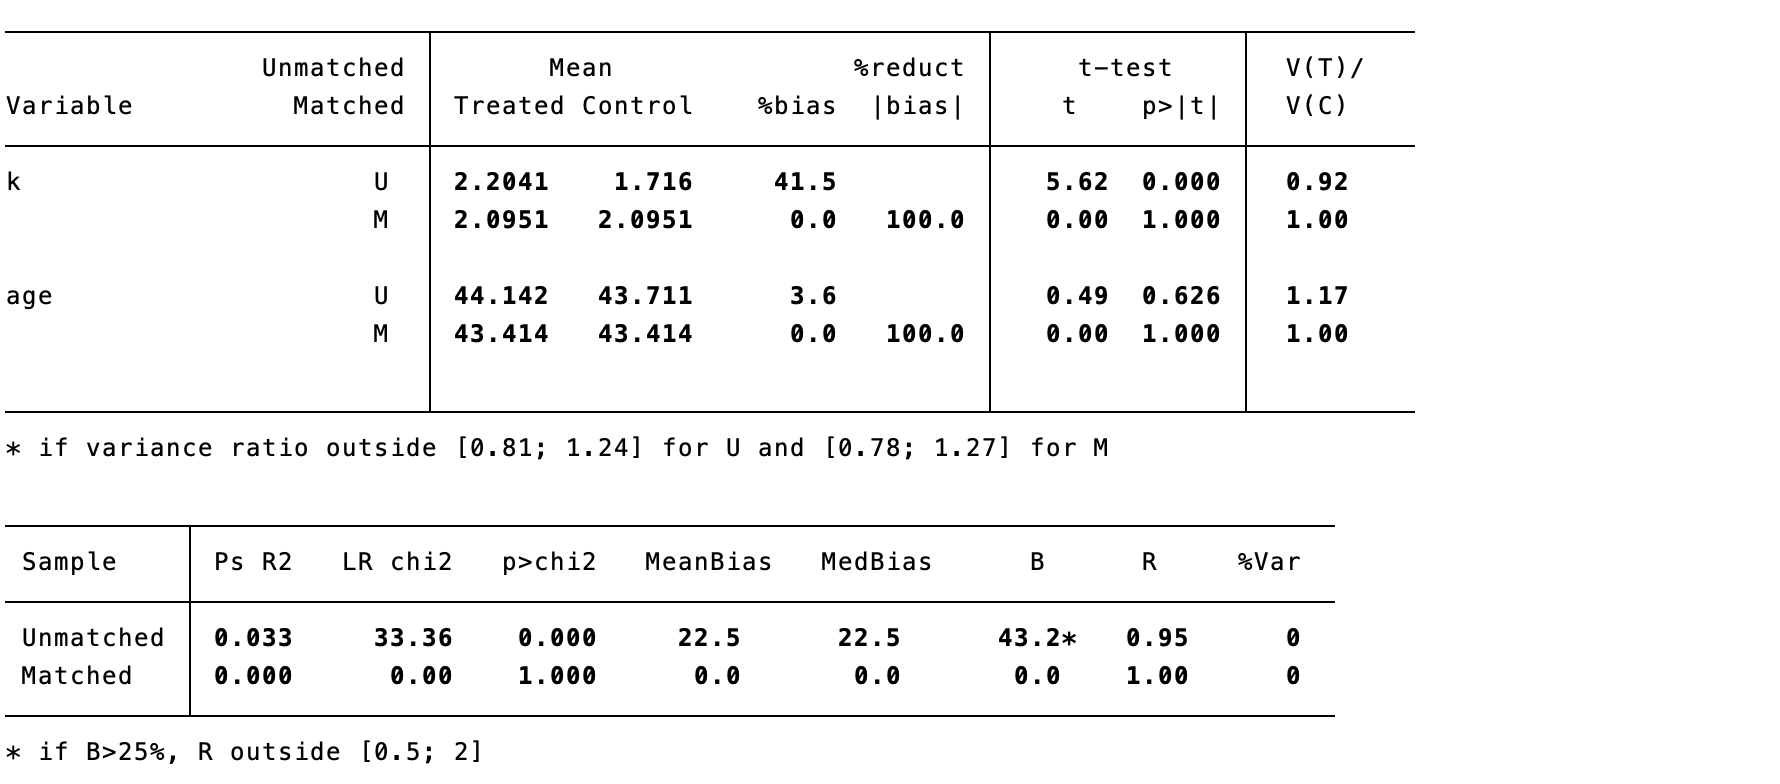
\includegraphics[width=1\linewidth,height=\textheight,keepaspectratio]{chapters/images/ch10-image8.png}

\end{tcolorbox}

\section{利用倾向性评分进行逆概率加权（inverse probability weighting,
IPW）}\label{ux5229ux7528ux503eux5411ux6027ux8bc4ux5206ux8fdbux884cux9006ux6982ux7387ux52a0ux6743inverse-probability-weighting-ipw}

给某每一个受试者分配一个权重，通过这样的一个权重我们就可以构建一个假人群，在这个假人群当中我们可以通过统计学的方法来证明不存在混杂效应，然后进行因果推断（图10.3）。例如，一个干预组中的患者，根据倾向性评分模型，只有25\%的概率为干预组，所以这个患者的权重为4。理由是他不仅代表自己，还代表4个``类似''他的人。对于对照组中的患者，若根据倾向性评分模型，有90\%的概率为干预组，则这个患者的权重为10。理由是他只有10\%的概率为对照组，他还代表10个``类似''他的人。

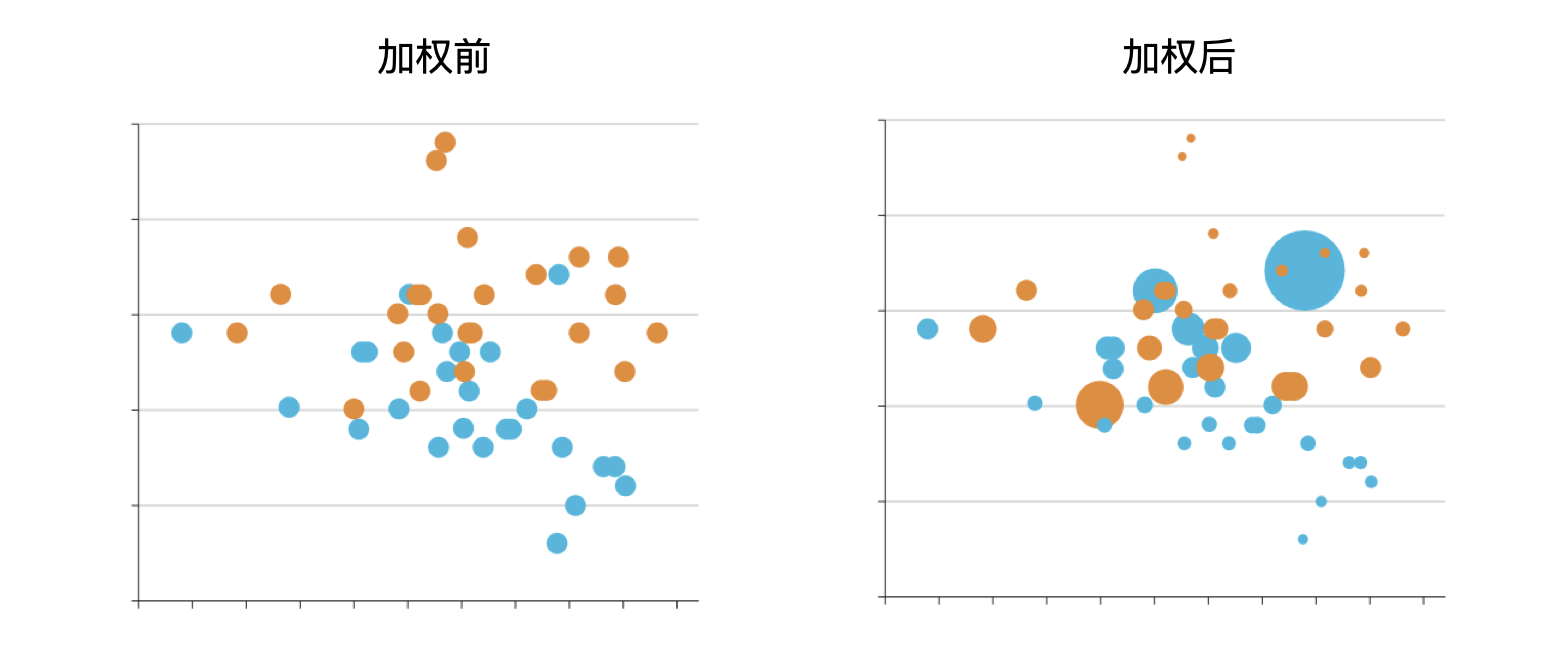
\includegraphics[width=1\linewidth,height=\textheight,keepaspectratio]{chapters/images/ch10-image9.png}

\textbf{图10.3 逆概率加权原理}

如果研究的问题只包含两种治疗方式（干预或对照），那么权重方程又可写成：

\[w_{ki}^{T=1}=\frac{1}{Pr(T=1\mid k_i)},\qquad w_{ki}^{T=0}=\frac{1}{1-Pr(T=1\mid k_i)}\]

计算权重后，将回归方程的权重指定为逆概率权重。

\begin{tcolorbox}[enhanced jigsaw, arc=.35mm, bottomrule=.15mm, breakable, colback=white, colframe=quarto-callout-note-color-frame, left=2mm, leftrule=.75mm, opacityback=0, rightrule=.15mm, toprule=.15mm]

\vspace{-3mm}\textbf{代码10.6}\vspace{3mm}

\begin{Shaded}
\begin{Highlighting}[]
\NormalTok{. }\KeywordTok{gen}\NormalTok{ ipweight = 1/\_pscore }\KeywordTok{if}\NormalTok{ Treatment == 1}
\NormalTok{. }\KeywordTok{replace}\NormalTok{ ipweight = 1/(1{-}\_pscore) }\KeywordTok{if}\NormalTok{ Treatment == 0}
\NormalTok{. }\KeywordTok{logistic}\NormalTok{ Outcome Treatment [}\KeywordTok{iweight}\NormalTok{ = ipweight], }\KeywordTok{vce}\NormalTok{(}\KeywordTok{robust}\NormalTok{)}
\end{Highlighting}
\end{Shaded}

\end{tcolorbox}

\begin{tcolorbox}[enhanced jigsaw, arc=.35mm, bottomrule=.15mm, breakable, colback=white, colframe=quarto-callout-note-color-frame, left=2mm, leftrule=.75mm, opacityback=0, rightrule=.15mm, toprule=.15mm]

\vspace{-3mm}\textbf{代码10.6输出}\vspace{3mm}

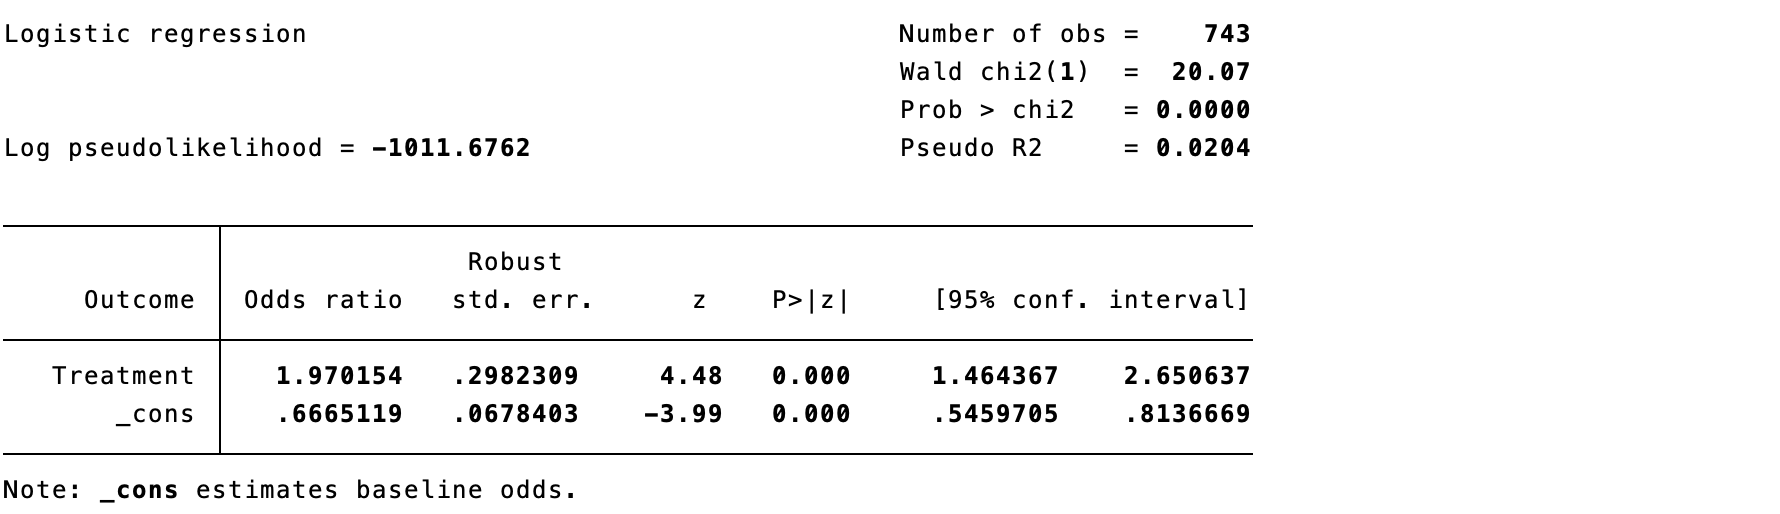
\includegraphics[width=1\linewidth,height=\textheight,keepaspectratio]{chapters/images/ch10-image10.png}

\end{tcolorbox}

然而，如果说某个样本的倾向性评分很小，其权重就会变得很大，从而导致因果效应估计引入了一个不稳定的因素，从而得出的推断方差较大。因此实践中，比较常用的是稳定的权重，给逆概率乘一个分子，即干预的总体概率（干预组）或者对照的总体概率（对照组），得出稳定的逆概率：稳定权重可缓和、但不能完全消除极端权重带来的不稳定性。应报告权重分布与有效样本量，并预先说明是否进行截尾、修剪或敏感性分析。

\[SW_{ki}^{T=1}=\frac{Pr(T=1)}{Pr(T=1\mid k_i)},\qquad SW_{ki}^{T=0}=\frac{1-Pr(T=1)}{1-Pr(T=1\mid k_i)}\]

\begin{tcolorbox}[enhanced jigsaw, arc=.35mm, bottomrule=.15mm, breakable, colback=white, colframe=quarto-callout-note-color-frame, left=2mm, leftrule=.75mm, opacityback=0, rightrule=.15mm, toprule=.15mm]

\vspace{-3mm}\textbf{代码10.7}\vspace{3mm}

\begin{Shaded}
\begin{Highlighting}[]
\NormalTok{. }\KeywordTok{gen}\NormalTok{ s\_ipweight = (1/\_pscore)*0.4516 }\KeywordTok{if}\NormalTok{ Treatment == 1}
\NormalTok{. }\KeywordTok{replace}\NormalTok{ s\_ipweight = 1/(1{-}\_pscore)*0.5484 }\KeywordTok{if}\NormalTok{ Treatment == 0}
\NormalTok{. }\KeywordTok{logistic}\NormalTok{ Outcome Treatment [}\KeywordTok{iweight}\NormalTok{ = s\_ipweight], }\KeywordTok{vce}\NormalTok{(}\KeywordTok{robust}\NormalTok{) }\KeywordTok{or}
\end{Highlighting}
\end{Shaded}

\end{tcolorbox}

\begin{tcolorbox}[enhanced jigsaw, arc=.35mm, bottomrule=.15mm, breakable, colback=white, colframe=quarto-callout-note-color-frame, left=2mm, leftrule=.75mm, opacityback=0, rightrule=.15mm, toprule=.15mm]

\vspace{-3mm}\textbf{代码10.7输出}\vspace{3mm}

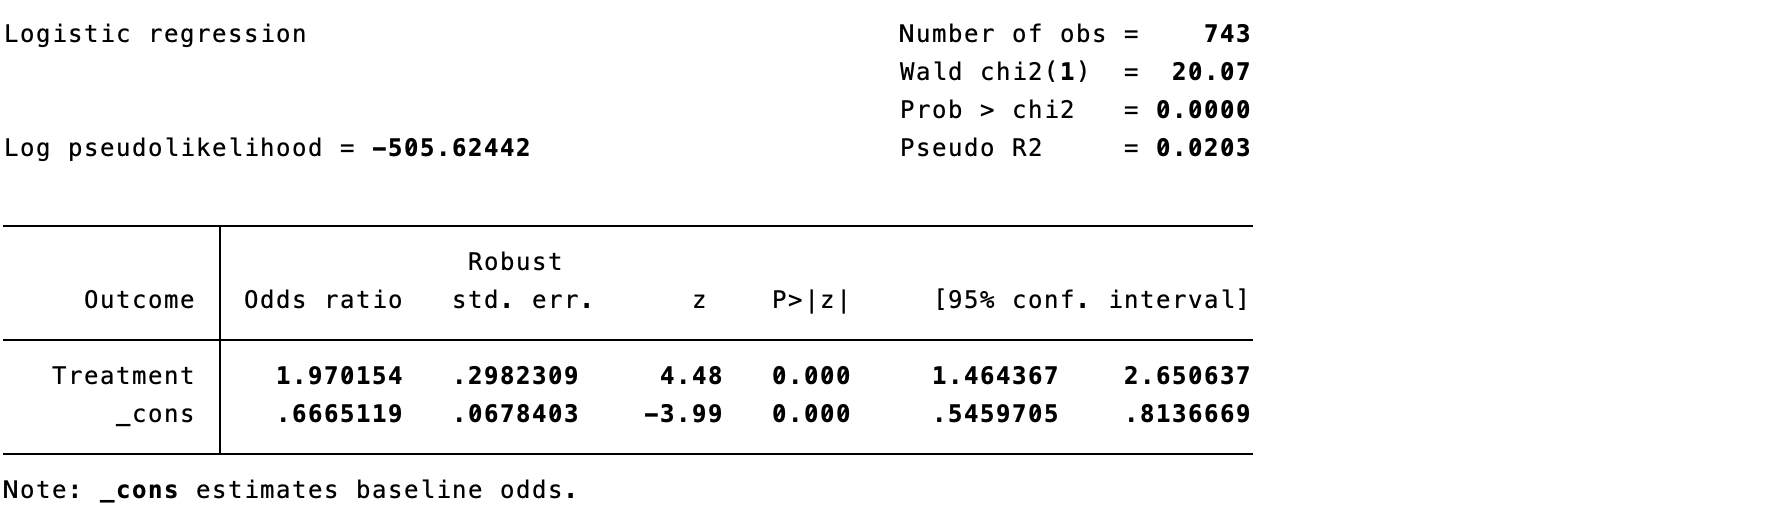
\includegraphics[width=1\linewidth,height=\textheight,keepaspectratio]{chapters/images/ch10-image11.png}

\end{tcolorbox}

通过标化的均数差值（standardized mean
difference，SMD）评估加权前后两组间协变量的差值。加权前两组的病例数分别为338和405，加权后为371.4和371.6。对于肿瘤侵袭性，加权前两组的差值为0.415，加权后为-0.002。一般，加权后的SMD需要控制在0.10之内。加权后病例数是加权伪样本量，并不等同于有效样本量。除
SMD 外，宜同时查看权重分布、有效样本量和协变量分布图。

\begin{tcolorbox}[enhanced jigsaw, arc=.35mm, bottomrule=.15mm, breakable, colback=white, colframe=quarto-callout-note-color-frame, left=2mm, leftrule=.75mm, opacityback=0, rightrule=.15mm, toprule=.15mm]

\vspace{-3mm}\textbf{代码10.8}\vspace{3mm}

\begin{Shaded}
\begin{Highlighting}[]
\NormalTok{. teffects ipw (Outcome) (Treatment }\KeywordTok{k}\NormalTok{ age, }\KeywordTok{logit}\NormalTok{)}
\NormalTok{. tebalance }\KeywordTok{summarize}
\end{Highlighting}
\end{Shaded}

\end{tcolorbox}

\begin{tcolorbox}[enhanced jigsaw, arc=.35mm, bottomrule=.15mm, breakable, colback=white, colframe=quarto-callout-note-color-frame, left=2mm, leftrule=.75mm, opacityback=0, rightrule=.15mm, toprule=.15mm]

\vspace{-3mm}\textbf{代码10.8输出}\vspace{3mm}

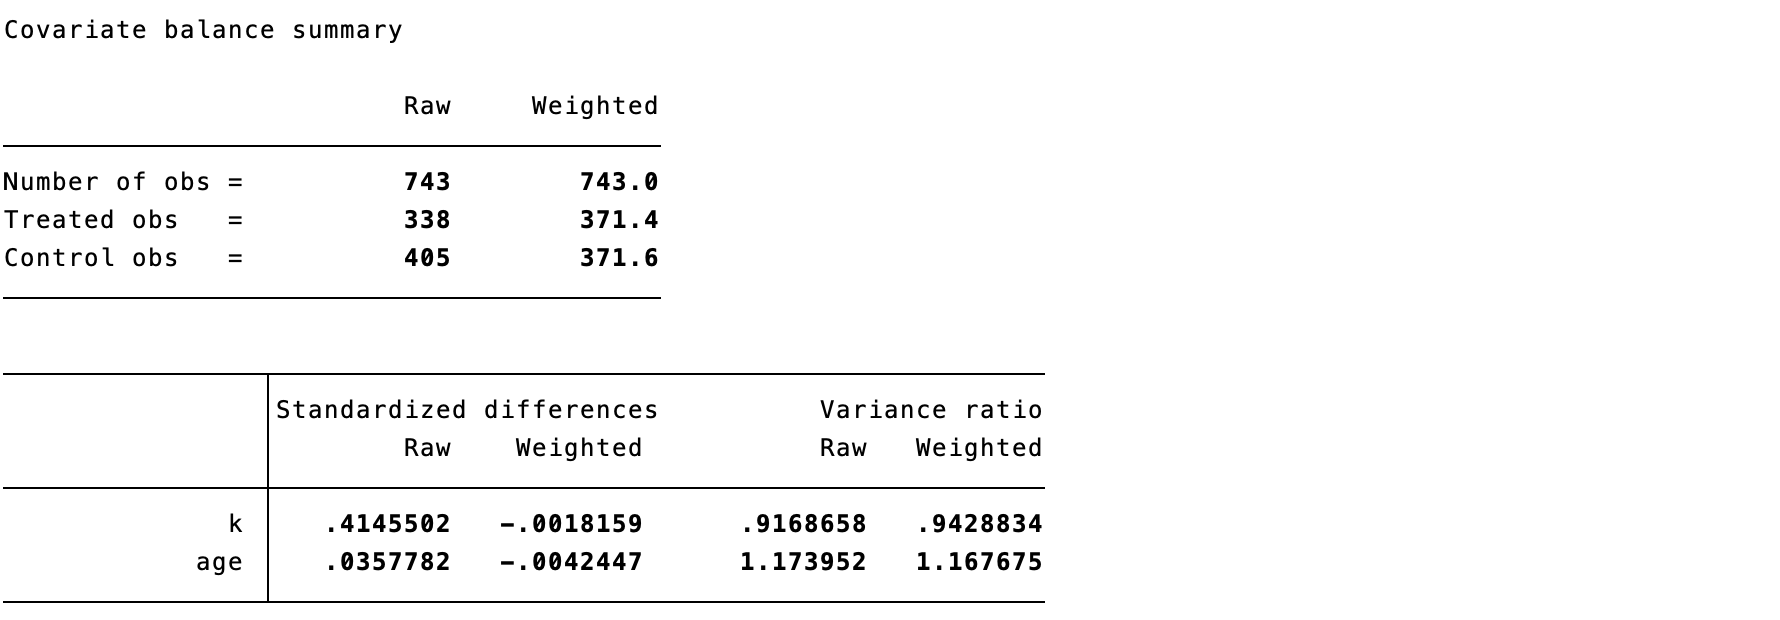
\includegraphics[width=1\linewidth,height=\textheight,keepaspectratio]{chapters/images/ch10-image12.png}

\end{tcolorbox}

\section{其他加权方法}\label{ux5176ux4ed6ux52a0ux6743ux65b9ux6cd5}

拟概率加权的问题是极端值影响结果，常规逆概率加权对治疗组的权重为1/PS，未治疗组为1/(1−PS)，使得某个样本的倾向性评分很小或者很大，其权重就会变得很大。虽然可用拟概率加权截尾方法（截掉加权后两边的极值，如第95百分位数对第99百分位数），但这种方法却不能保证截尾位置是否合适，且样本量也减少了。

\subsection{重叠加权（Overlap
weighting）}\label{ux91cdux53e0ux52a0ux6743overlap-weighting}

重叠加权给予每个患者分配与该患者属于相反治疗组概率的权重，克服了这些限制。具体来说，接受治疗的患者以未接受治疗的概率【1−PS】为权重，而未接受治疗的患者以接受治疗的概率【PS】为权重。这些权值使得PS接近于1或者0的离群值不会像拟概率加权那样主导结果和降低精度。而那些人群特征在两种治疗方法中都兼容的患者则相对贡献更大，由此产生的目标人群模仿了实用性随机试验的特点。该方法的目标人群是两种治疗均具有合理可能性的重叠（临床均势）人群，而非整个入组人群；因此其效应应与所选
estimand 一并报告。

这种加权方法在结构上可以产生治疗组和参照组之间的精确协变量平衡。然而，推断的目标是重叠人群中的平均治疗效应（ATO），它可能与整个研究人群中的ATT或ATE不同。强调在临床均势情况下对患者进行比较（不考虑肯定会采取干预或肯定会采取对照的情况），结果可见效应较前面几种方法有所下降。
效应估计的改变通常源于目标人群改变，不能简单解释为效应``下降''。

\begin{tcolorbox}[enhanced jigsaw, arc=.35mm, bottomrule=.15mm, breakable, colback=white, colframe=quarto-callout-note-color-frame, left=2mm, leftrule=.75mm, opacityback=0, rightrule=.15mm, toprule=.15mm]

\vspace{-3mm}\textbf{代码10.9}\vspace{3mm}

\begin{Shaded}
\begin{Highlighting}[]
\NormalTok{. }\KeywordTok{gen}\NormalTok{ o\_weight = 1 {-} \_pscore }\KeywordTok{if}\NormalTok{ Treatment == 1}
\NormalTok{. }\KeywordTok{replace}\NormalTok{ o\_weight = \_pscore }\KeywordTok{if}\NormalTok{ Treatment == 0}
\NormalTok{. }\KeywordTok{logistic}\NormalTok{ Outcome Treatment [}\KeywordTok{iweight}\NormalTok{ = o\_weight], }\KeywordTok{vce}\NormalTok{(}\KeywordTok{robust}\NormalTok{) }\KeywordTok{or}
\end{Highlighting}
\end{Shaded}

\end{tcolorbox}

\begin{tcolorbox}[enhanced jigsaw, arc=.35mm, bottomrule=.15mm, breakable, colback=white, colframe=quarto-callout-note-color-frame, left=2mm, leftrule=.75mm, opacityback=0, rightrule=.15mm, toprule=.15mm]

\vspace{-3mm}\textbf{代码10.9输出}\vspace{3mm}

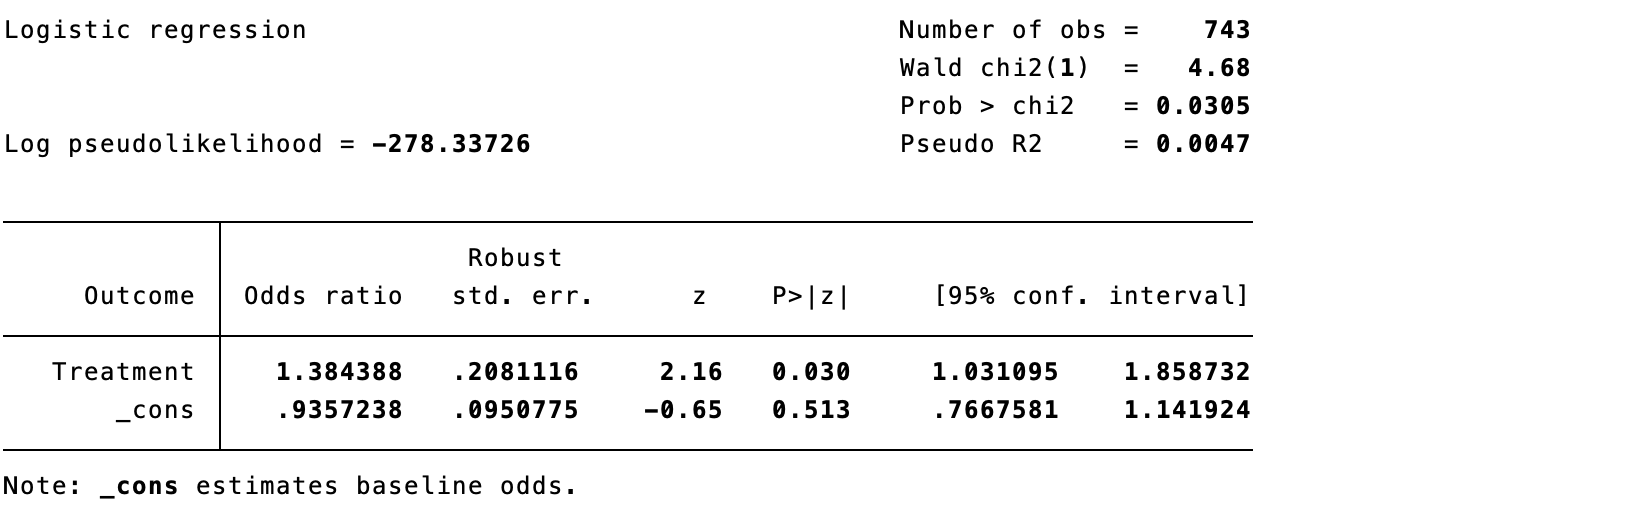
\includegraphics[width=1\linewidth,height=\textheight,keepaspectratio]{chapters/images/ch10-image13.png}

\end{tcolorbox}

\subsection{匹配加权（Match
weighting）}\label{ux5339ux914dux52a0ux6743match-weighting}

这种方法是将接受干预或接受治疗的概率中较低的一个与实际接受治疗的预测概率之比对患者进行加权。匹配加权给予接受治疗的患者的权重为【Minimum(PS,
1 − PS) / PS】，而未接受治疗的患者以接受治疗的权重【Minimum(PS, 1 − PS)
/ (1 −
PS)】。此方法排除了极端的权重，消除了权重截断的需要。当两个组群体大小相同，倾向性评分分布有很好的重叠时，推断的目标接近整个人口中的ATE；当两个组群体大小不均，但倾向性评分分布有很好的重叠时，推断的目标接近样本数较少群体中的ATT。在倾向性评分分布重叠度有限的情况下，这种方法的推断目标是在重叠子群体中进行治疗效果估计。匹配加权的估计目标取决于样本构成与倾向评分重叠的具体形态，报告时不宜仅以接近
ATE 或 ATT 代替对目标分布的描述。

\begin{tcolorbox}[enhanced jigsaw, arc=.35mm, bottomrule=.15mm, breakable, colback=white, colframe=quarto-callout-note-color-frame, left=2mm, leftrule=.75mm, opacityback=0, rightrule=.15mm, toprule=.15mm]

\vspace{-3mm}\textbf{代码10.10}\vspace{3mm}

\begin{Shaded}
\begin{Highlighting}[]
\NormalTok{. }\KeywordTok{gen}\NormalTok{ m\_weighting = }\FunctionTok{min}\NormalTok{(\_pscore, 1{-}\_pscore)/\_pscore}
\NormalTok{. }\KeywordTok{replace}\NormalTok{ m\_weighting = }\FunctionTok{min}\NormalTok{(\_pscore, 1{-}\_pscore)/(1{-}\_pscore) }\KeywordTok{if}\NormalTok{ Treatment == 0}
\NormalTok{. }\KeywordTok{logit}\NormalTok{ Outcome Treatment [}\KeywordTok{iweight}\NormalTok{ = m\_weighting], }\KeywordTok{vce}\NormalTok{(}\KeywordTok{robust}\NormalTok{) }\KeywordTok{or}
\end{Highlighting}
\end{Shaded}

\end{tcolorbox}

\begin{tcolorbox}[enhanced jigsaw, arc=.35mm, bottomrule=.15mm, breakable, colback=white, colframe=quarto-callout-note-color-frame, left=2mm, leftrule=.75mm, opacityback=0, rightrule=.15mm, toprule=.15mm]

\vspace{-3mm}\textbf{代码10.10输出}\vspace{3mm}

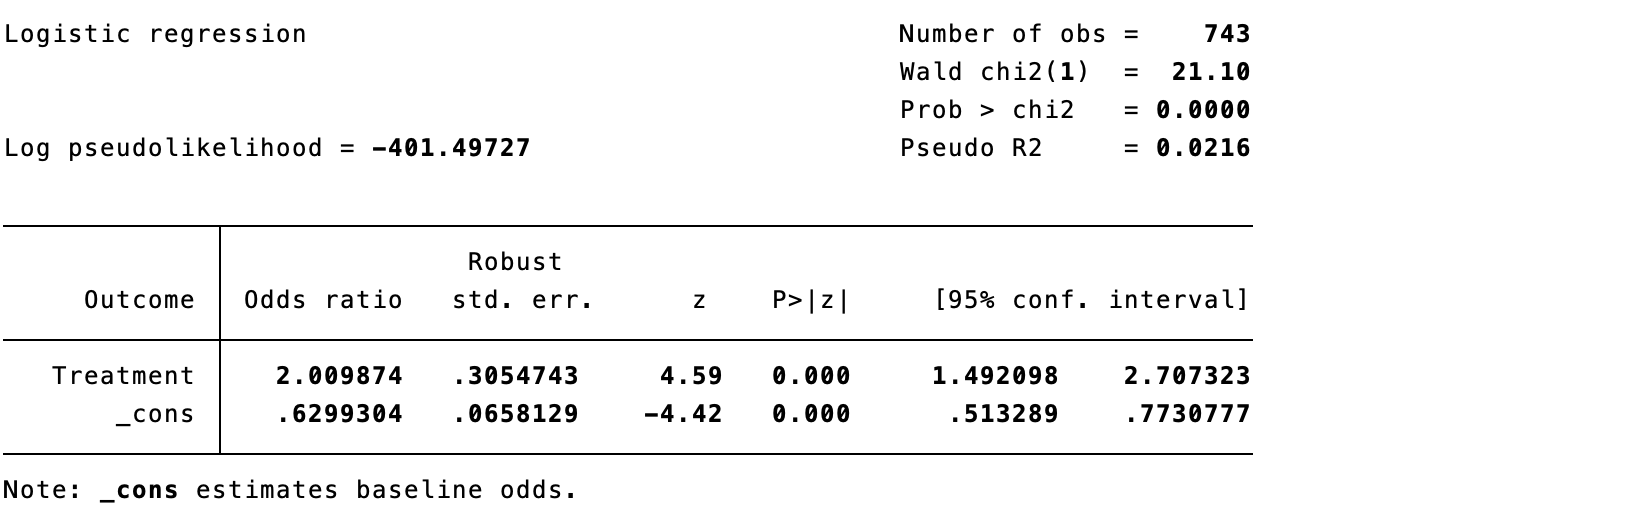
\includegraphics[width=1\linewidth,height=\textheight,keepaspectratio]{chapters/images/ch10-image14.png}

\end{tcolorbox}

\subsection{精细分层加权（Fine stratification
weighting）}\label{ux7cbeux7ec6ux5206ux5c42ux52a0ux6743fine-stratification-weighting}

以平均治疗效果为目标的精细分层加权不直接使用倾向性评分来计算加权，而是用倾向性评分来创建精细分层。分层规则为固定的概率宽度（如0-0.02为分层1，0.02-0.04为分层2，以此类推）。没有干预患者或对照患者的分层被剔除后，根据剩余每个分层中的患者总数，计算出干预和对照组的权重。

以治疗人群中的平均治疗效果为目标的精细分层与上述精细分层方法类似，倾向评分被用来创建精细分层，但治疗组的权重被设定为1，对照组患者根据其所致分层中的干预组患者数量进行重新加权。

\subsection{标准化死亡率加权（Standardized mortality ratio
weighting）}\label{ux6807ux51c6ux5316ux6b7bux4ea1ux7387ux52a0ux6743standardized-mortality-ratio-weighting}

这种方法是将接受治疗的病人的权重设置为1，并通过倾向性评分给予对照组患者的权重为【PS/（1-PS）】。与逆概率加权类似，标准化死亡率加权有可能受到极端权重的影响，因为倾向分数被直接用于计算权重。如果观察到大权重，可以考虑截断权重。

\begin{tcolorbox}[enhanced jigsaw, arc=.35mm, bottomrule=.15mm, breakable, colback=white, colframe=quarto-callout-note-color-frame, left=2mm, leftrule=.75mm, opacityback=0, rightrule=.15mm, toprule=.15mm]

\vspace{-3mm}\textbf{代码10.11}\vspace{3mm}

\begin{Shaded}
\begin{Highlighting}[]
\KeywordTok{gen}\NormalTok{ smr\_weighting = 1}
\NormalTok{. }\KeywordTok{replace}\NormalTok{ smr\_weighting = \_pscore/(1{-}\_pscore) }\KeywordTok{if}\NormalTok{ Treatment == 0}
\NormalTok{. }\KeywordTok{logit}\NormalTok{ Outcome Treatment [}\KeywordTok{iweight}\NormalTok{ = smr\_weight], }\KeywordTok{vce}\NormalTok{(}\KeywordTok{robust}\NormalTok{) }\KeywordTok{or}
\end{Highlighting}
\end{Shaded}

\end{tcolorbox}

\begin{tcolorbox}[enhanced jigsaw, arc=.35mm, bottomrule=.15mm, breakable, colback=white, colframe=quarto-callout-note-color-frame, left=2mm, leftrule=.75mm, opacityback=0, rightrule=.15mm, toprule=.15mm]

\vspace{-3mm}\textbf{代码10.11输出}\vspace{3mm}

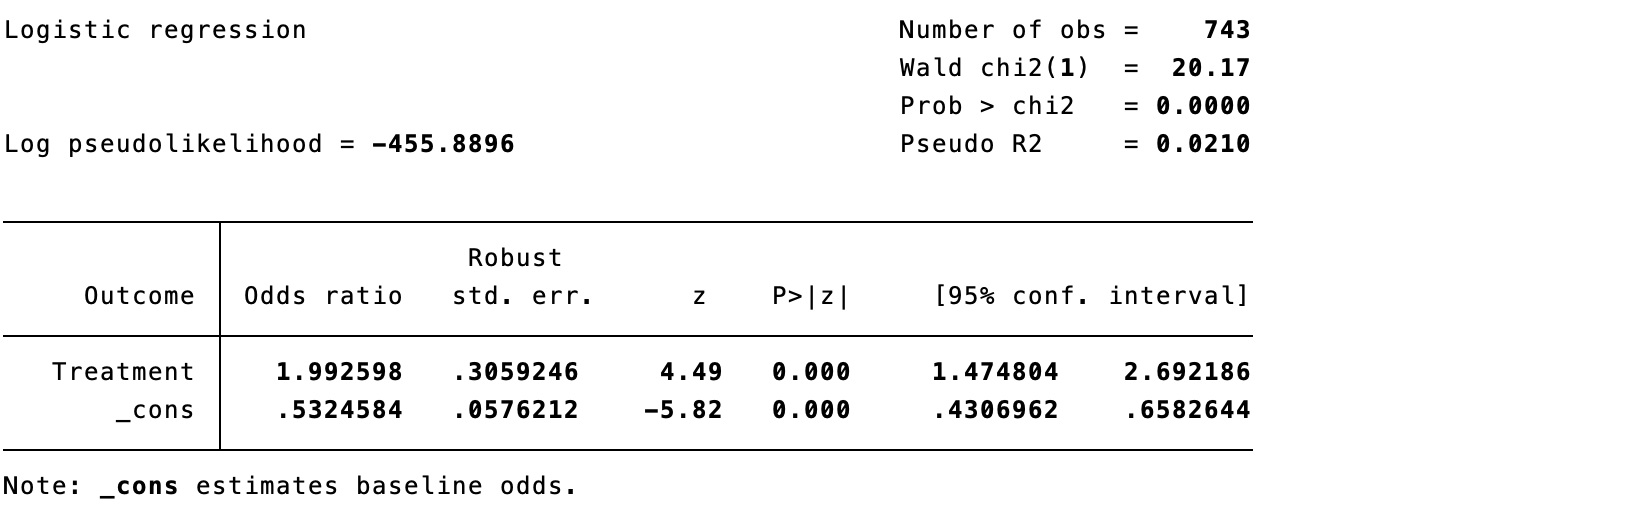
\includegraphics[width=1\linewidth,height=\textheight,keepaspectratio]{chapters/images/ch10-image15.png}

\end{tcolorbox}

\section{以倾向评分为基础的各种方法的选择}\label{ux4ee5ux503eux5411ux8bc4ux5206ux4e3aux57faux7840ux7684ux5404ux79cdux65b9ux6cd5ux7684ux9009ux62e9}

干预组样本倾向性评分在预先指定的范围内（卡尺）将其与固定数量的对照值相匹配，这通常是使用倾向性评分进行混杂调整的首选方法。然而，这种方法有一个重要的局限性，即可能放弃未匹配的样本。在倾向性评分匹配后，协变量的不平衡性可能会增加。匹配并非普遍首选；若旨在整个可比研究样本的
ATE
或希望尽量保留样本，可在重叠和稳定性良好的前提下考虑加权。方法应由目标
estimand、重叠程度、可接受的样本损失及平衡结果共同决定。

对倾向性评分进行加权有几个优点。首先，与匹配不同，加权在分析中保留了大多数样本，因此，在估计治疗效果时可以提供更高的精度。其次，与倾向性评分的回归调整不同，加权很容易使治疗人群和参照人群之间的平衡得到透明的报告。最后，对倾向性评分的加权可以说是在分析中使用倾向性评分的最灵活的方法，有多种可用的变化，可以针对特定人群进行推断。除了使用逆概率治疗加权外，上述新的方法（包括倾向性评分精细分层加权、匹配加权和重叠加权）都可以克服传统加权方法的重要局限性。

推断目标（estimand）是指估计的治疗效果所适用的患者人群。研究者在构思特定研究的推断目标时应考虑以下核心问题------用感兴趣的干预方法治疗研究中所有符合条件的患者是否可行？如果可行，那么推断的目标就可以定义为平均治疗效果（ATE）。如果不可行，即临床上不会给人群中符合条件的每一个人提供治疗，只有具有某些特征的、并实际接受干预的患者才是理想的干预对象，因此推断的目标可定义为治疗人群的平均治疗效果（ATT）。下表总结了每种加权方法的主要特点。

\textbf{表10.1几种不同基于倾向性评分的加权方法}

{\def\LTcaptype{none} % do not increment counter
\begin{longtable}[]{@{}
  >{\raggedright\arraybackslash}p{(\linewidth - 8\tabcolsep) * \real{0.2000}}
  >{\raggedright\arraybackslash}p{(\linewidth - 8\tabcolsep) * \real{0.2000}}
  >{\raggedright\arraybackslash}p{(\linewidth - 8\tabcolsep) * \real{0.2000}}
  >{\raggedright\arraybackslash}p{(\linewidth - 8\tabcolsep) * \real{0.2000}}
  >{\raggedright\arraybackslash}p{(\linewidth - 8\tabcolsep) * \real{0.2000}}@{}}
\toprule\noalign{}
\begin{minipage}[b]{\linewidth}\raggedright
方法
\end{minipage} & \begin{minipage}[b]{\linewidth}\raggedright
干预组
\end{minipage} & \begin{minipage}[b]{\linewidth}\raggedright
对照组
\end{minipage} & \begin{minipage}[b]{\linewidth}\raggedright
推断目标
\end{minipage} & \begin{minipage}[b]{\linewidth}\raggedright
说明
\end{minipage} \\
\midrule\noalign{}
\endhead
\bottomrule\noalign{}
\endlastfoot
逆概率加权 & 1/PS & 1/(1-PS) & ATE &
明确的推断目标，模拟了随机对照试验。然而，因为PS是直接用来创建权重，通常会出现极端的权重，可采用截尾解决极端权重。 \\
标准死亡率加权 & 1 & PS/(1-PS) & ATT &
加权是通过对照组的倾向性评分进行的，可以自然地扩展到有\textgreater2个治疗组的情况。可能需要对权重进行修剪。 \\
重叠加权 & (1-PS) & PS & 重叠人群中的ATE &
避免了极端权重。这种方法的目标人群可以被描述为重叠人群或具有合理临床均衡性人群中的治疗效果估计，而这些人群并不反映在常规护理中接受治疗的整个研究人群。 \\
匹配加权 & Min(PS, 1-PS) / PS & Min(PS, 1-PS) / (1-PS) & 较小组别中的ATT
&
避免了极端权重。可以自然地扩展到有两个以上治疗组的情况。当组别大小相同且PS分布有很好的重叠时，推断目标接近整个人群的ATE；当组别大小不均但PS分布有很好的重叠时，推断目标接近较小组别中的ATT。 \\
\end{longtable}
}

选择倾向性评分加权方法进行混杂调整时有若干考虑：

\subsection{正确规范倾向性评分模型}\label{ux6b63ux786eux89c4ux8303ux503eux5411ux6027ux8bc4ux5206ux6a21ux578b}

在使用倾向性评分进行混杂调整的分析中，第一个关键步骤是避免倾向性评分模型的错误。由于研究者不可能知道治疗分配与所有协变量之间的真正结构性关联，因此，在从简单的逻辑回归模型中估计倾向性评分时，可能会出现模型的错误指定。可采用机器学习方法（参考）作为替代方法。
无论采用哪种方法构建倾向性评分模型，研究人员都应强调将结果风险因素纳入模型，并从模型中排除与结果无关但与治疗相关的强预测因素，以避免倾向性评分接近0或1。基于倾向分数分层的加权方法可能对倾向分数模型的错误指定更为稳健，因为它可以被概念化为倾向分数加权的半参数模型，只使用分数来创建分层，然后使用每个分层中的观察值计数来得出权重。倾向评分模型的优劣应由匹配或加权后的平衡判断，而非
c
统计量或预测精度。对于连续或非线性协变量，可考虑样条、交互项或灵活的机器学习模型，并保持模型选择与结局分析相对独立。

\subsection{评估暴露组和参照组之间的倾向性评分分布重叠情况}\label{ux8bc4ux4f30ux66b4ux9732ux7ec4ux548cux53c2ux7167ux7ec4ux4e4bux95f4ux7684ux503eux5411ux6027ux8bc4ux5206ux5206ux5e03ux91cdux53e0ux60c5ux51b5}

倾向性评分分布的高重叠度通常表明，在比较组之间的治疗选择中存在合理程度的临床等值。在考虑基于倾向评分的加权时，对非重叠区域进行修剪以确保限制在患者接受任何一种治疗的概率不为零的区域尤为重要。接近0或1的概率可能会导致较大的权重，从而过度影响分析，因为非典型情况下的患者肯定会接受这两种治疗中的一种。如果在修剪了非重叠区域后，丢失了很大一部分样本，这可能表明分布之间的重叠度不够。此外，由于不重叠而通过修剪排除观测值，会导致研究人群的构成发生重要变化，因此，可能会改变推断的目标。修剪阈值会改变目标人群，建议同时报告修剪规则、被排除人数与修剪前后的协变量分布，并通过不同合理阈值开展敏感性分析。

\subsection{推断目标的选择}\label{ux63a8ux65adux76eeux6807ux7684ux9009ux62e9}

由于基于倾向性评分的不同加权方法会导致针对不同人群的估计，研究者应密切关注他们的推断目标并选择相应的加权方法。人群平均治疗效应的目的是使治疗组和参照组的协变量分布相互类似，并与整个研究样本的分布类似。受治人群中的平均治疗效果ATT旨在使参考组中协变量的分布与治疗组中观察到的分布相似。具有临床均势子集的平均治疗效果，受倾向性评分分布重叠的影响很大，目标是总体人群中具有临床均势性子集的平均治疗效果（即排除了肯定会予以干预组或者肯定会予以对照组的患者，在这个子集中，临床上病人接受干预或对照有争议）

某些加权方法很容易扩展到两个以上治疗组的情况，包括逆概率加权、匹配权重和标准死亡率加权。所有这些方法都涉及到在多元逻辑回归模型中为三个或更多的治疗产生倾向性分数。逆概率加权是根据实际接受治疗的倾向性的倒数来计算的，无需考虑治疗组的数量如何。对于三组或更多组的匹配权重，分子包括每个病人的所有可用倾向分数的最小值，分母包括实际接受治疗的倾向。对于标准死亡率加权，研究者可以通过将接受目标治疗的病人的权重设置为1，并将其他治疗组的权重计算为目标治疗的倾向与实际接受的治疗的倾向之比，来确定特定治疗组的ATT。

\section{利用倾向性评分进行因果推断的局限性}\label{ux5229ux7528ux503eux5411ux6027ux8bc4ux5206ux8fdbux884cux56e0ux679cux63a8ux65adux7684ux5c40ux9650ux6027}

其局限性源于倾向性评分的方程，若估计错误会导致后续一系列的因果估计的错误。其次，存在未测量的混杂因素，利用倾向性评分也同样遗漏这些未测量的混杂因素，导致因果推断错误。第三、倾向性评分匹配需要考虑普适性问题，因为只有匹配的样本才能够被正确地估计因果效应，没有匹配的样本中的因果效应无法估计。未测量混杂无法由倾向评分修复，应结合领域知识、定量偏倚分析或
E-value
等敏感性分析讨论其潜在影响；外推到未匹配或缺乏重叠的人群时应谨慎。

\section{参考文献}\label{ux53c2ux8003ux6587ux732e-7}

\begin{enumerate}
\def\labelenumi{\arabic{enumi}.}
\tightlist
\item
  Rosenbaum PR, Rubin DB. The central role of the propensity score in
  observational studies for causal effects. \emph{Biometrika}.
  1983;70(1):41-55. doi:10.1093/biomet/70.1.41.
\item
  Brookhart MA, Schneeweiss S, Rothman KJ, et al.~Variable selection for
  propensity score models. \emph{Am J Epidemiol}.
  2006;163(12):1149-1156. doi:10.1093/aje/kwj149. PMID: 16624967.
\item
  Austin PC. Balance diagnostics for comparing the distribution of
  baseline covariates between treatment groups in propensity-score
  matched samples. \emph{Stat Med}. 2009;28(25):3083-3107.
  doi:10.1002/sim.3697. PMID: 19757444.
\item
  Austin PC. Optimal caliper widths for propensity-score matching when
  estimating differences in means and differences in proportions in
  observational studies. \emph{Pharm Stat}. 2011;10(2):150-161.
  doi:10.1002/pst.433. PMID: 20925139.
\item
  Austin PC, Stuart EA. Moving towards best practice when using inverse
  probability of treatment weighting (IPTW) using the propensity score
  to estimate causal treatment effects in observational studies.
  \emph{Stat Med}. 2015;34(28):3661-3679. doi:10.1002/sim.6607. PMID:
  26238958.
\item
  Deb S, Austin PC, Tu JV, et al.~A review of propensity-score methods
  and their use in cardiovascular research. \emph{Can J Cardiol}.
  2016;32(2):259-265. doi:10.1016/j.cjca.2015.05.015. PMID: 26315351.
\item
  Li F, Thomas LE, Li F. Addressing extreme propensity scores via the
  overlap weights. \emph{Am J Epidemiol}. 2019;188(1):250-257.
  doi:10.1093/aje/kwy201. PMID: 30189042.
\item
  Elze MC, Gregson J, Baber U, et al.~Comparison of propensity score
  methods and covariate adjustment: evaluation in 4 cardiovascular
  studies. \emph{J Am Coll Cardiol}. 2017;69(3):345-357.
  doi:10.1016/j.jacc.2016.10.060. PMID: 28104076.
\item
  Garrido MM, Kelley AS, Paris J, et al.~Methods for constructing and
  assessing propensity scores. \emph{Health Serv Res}.
  2014;49(5):1701-1720. doi:10.1111/1475-6773.12182. PMID: 24779867.
\item
  VanderWeele TJ, Ding P. Sensitivity analysis in observational
  research: introducing the E-value. \emph{Ann Intern Med}.
  2017;167(4):268-274. doi:10.7326/M16-2607. PMID: 28693043.
\end{enumerate}

\bookmarksetup{startatroot}

\chapter{工具变量法}\label{ux5de5ux5177ux53d8ux91cfux6cd5}

采用回归以及倾向性评分进行因果推断的最大局限性是存在未观察的混杂因素时，通过这两大类方法无法直接进行。
工具变量并不会自动消除未测量混杂；它把识别任务转化为对工具变量有效性的强假设。若这些假设不可信，IV
估计同样可能有偏。

\section{工具变量法}\label{ux5de5ux5177ux53d8ux91cfux6cd5-1}

这时引入工具变量 Z，借此估计 X 到 Y 的因果关系。工具变量 Z 通过影响 X
而间接影响因变量 Y。如果工具变量 Z 和 X 密切相关，那么，只要工具变量 Z
有了变化，就必然会对 X 产生变化。如果 X 和 Y 之间真的存在因果关系，那么
Z 对 X 带来的冲击也就势必传递到 Y。这样，在一系列的假说之下，只要 Z 对 Y
的间接冲击能够被统计证明是显著的，我们就可以推断出 X 对 Y
有因果关系。利用对 Z 与 X 相关的估算，以及 Z 与 Y
相关的估算，就可以推导出 X 和 Y 之间真实关系的大小。 相关性本身只说明 Z
能预测
X，并不等于工具变量有效；因果解释还取决于独立性和排除限制。对于线性模型，单个有效工具变量的
Wald 比值可理解为 Z 对 Y 的效应除以 Z 对 X
的效应，但二者均需有足够精度。

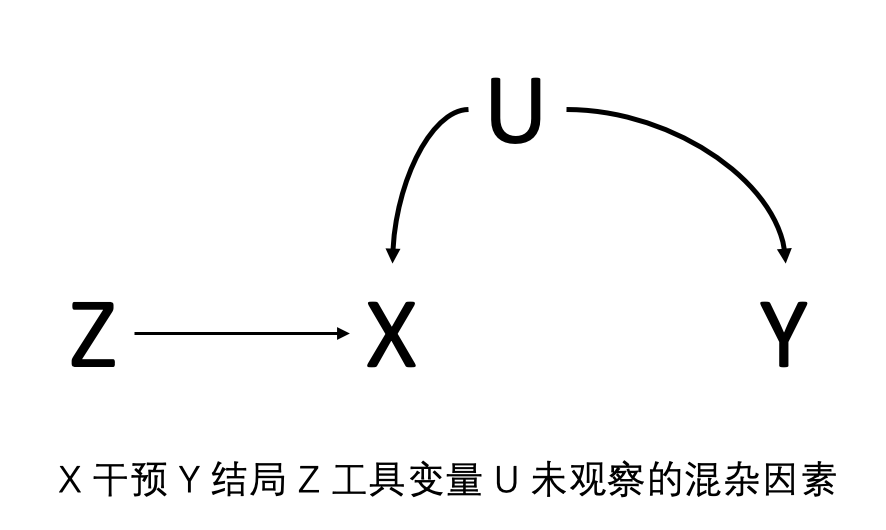
\includegraphics[width=0.42\linewidth,height=\textheight,keepaspectratio]{chapters/images/ch11-image1.png}

\textbf{图11.1 工具变量法示意图}

然而，工具变量的成立需要满足三个统计学假设：

\begin{enumerate}
\def\labelenumi{\arabic{enumi}.}
\tightlist
\item
  工具变量与干预是相关的，即 Z 和 X 相关；
\item
  工具变量对结局的影响只能通过干预来实现，Z 到 Y 的影响只能通过 A
  来实现的，而不能通过其他路径去实现；
\item
  工具变量与结局没有共同的原因，即 Z 和 Y 之间没有混杂因素。
  在二元工具变量和二元处理的常用解释下，若希望把结果解释为``依从者''的局部平均处理效应（LATE），还需加入单调性假设：不存在因工具变量取值改变而总是反向接受处理的个体。Hernán
  与 Robins（2006）及 Baiocchi
  等（2014）强调，这些假设多数不能由数据本身证明。
\end{enumerate}

在随机对照研究中，工具变量可以理解为随机分配。案例9.1假设为随机对照试验，Z
是随机分配为内窥镜组和显微镜组，X 为实际接受内窥镜手术和显微镜手术，Y
是手术后内分泌缓解。随机对照研究中的意向性分析所得意向性效应即是 Z 对 Y
的效应，随机分配后不管受试者是否依从所分配的方案，只考虑随机的结果。而符合方案分析得出的符合方案效应就是
X 到 Y
的效应，如果随机分配后的依从性是100\%，则符合方案效应等于意向性效应。非随机对照研究中的因果效应取决于所采用的工具变量、识别假设与目标
estimand，不能直接等同于随机试验中的符合方案效应。

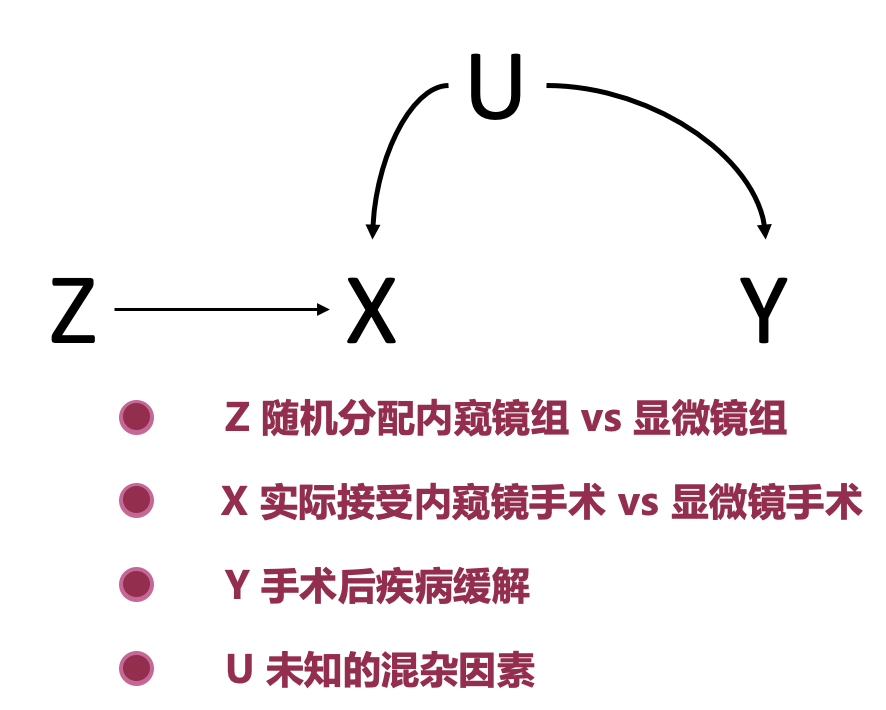
\includegraphics[width=0.42\linewidth,height=\textheight,keepaspectratio]{chapters/images/ch11-image2.png}

\textbf{图11.2 随机分配作为工具变量}

\section{工具变量法的实际应用}\label{ux5de5ux5177ux53d8ux91cfux6cd5ux7684ux5b9eux9645ux5e94ux7528}

研究饮酒是否会导致冠脉综合症？X 是饮酒，Y 是冠脉综合症，U
是未观察到的一些混杂因素，比如说饮酒的人一般都会吸烟，吸烟会导致冠脉综合症。而饮酒本身无法进行随机分配。这时，可以引入工具变量
Z，表示与酒精代谢有关的基因型，如果患者携带酒精代谢差的基因型，一般来说饮酒量会比较少，如果能通过基因表型分析获取
Z 和 X 的关系，获取 Z 和 Y 的关系，就可以估算出 X 与 Y 的关系。
遗传工具变量还须特别讨论水平多效性、群体分层、亲代效应和选择偏倚；任一因素都可能产生
Z 到 Y
的非经由饮酒的路径，因此不能仅凭基因与饮酒相关就断言工具变量有效。

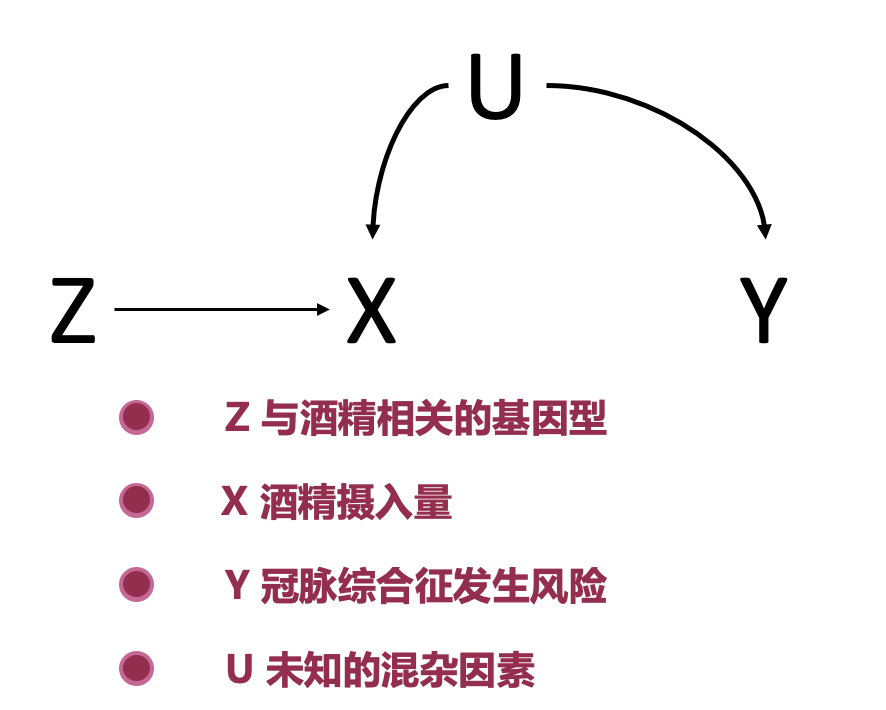
\includegraphics[width=0.42\linewidth,height=\textheight,keepaspectratio]{chapters/images/ch11-image3.png}

\textbf{图11.3 遗传变异作为候选工具变量}

研究HIV感染患者中使用不同的逆转录逆转录抗病毒的疗法，预防AIDS或者死亡的因果关系，利用年历时间作为工具变量。在不同时间窗内采纳的治疗方法不同，借此可以估算对结局的效应。然而，年历时间作为工具变量时，工具变量与结局变量之间可能存在一些混杂因素，如年历可能通过其他医学技术的革新导致死亡率的下降。
年历时间往往尤其容易违反排除限制：诊断技术、围手术期管理、病例构成和随访制度可能同时随时间改变。将其用作工具变量前，应预先画出因果图、说明每一条替代路径，并以敏感性分析检验结论对这些设定的依赖。

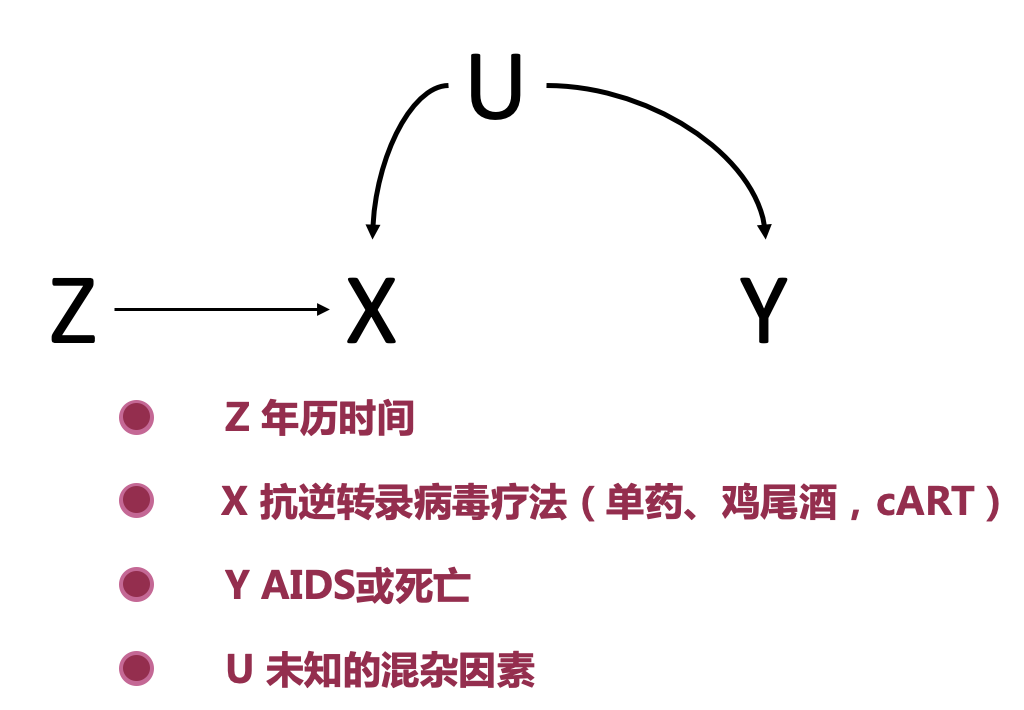
\includegraphics[width=0.48\linewidth,height=\textheight,keepaspectratio]{chapters/images/ch11-image4.png}

\textbf{图11.4 年历时间作为候选工具变量}

看电视过多是否会引发小儿自闭症？电视的普及与小儿自闭症发生率的攀升几乎同步。然而，有自闭倾向的儿童可能更经常看电视，而不喜欢户外活动或与人交往。使用降雨量作为电视观看时间的工具变量。即降雨越多的地区，人们待在室内的时间越长，故看电视时间也长；而降雨量很可能只通过看电视时间而影响被解释变量。
降雨量也未必天然有效：它可能通过户外活动、感染暴露、就医可及性或地区社会经济条件影响结局。所谓``自然工具''仍须针对研究场景逐项论证独立性和排除限制。

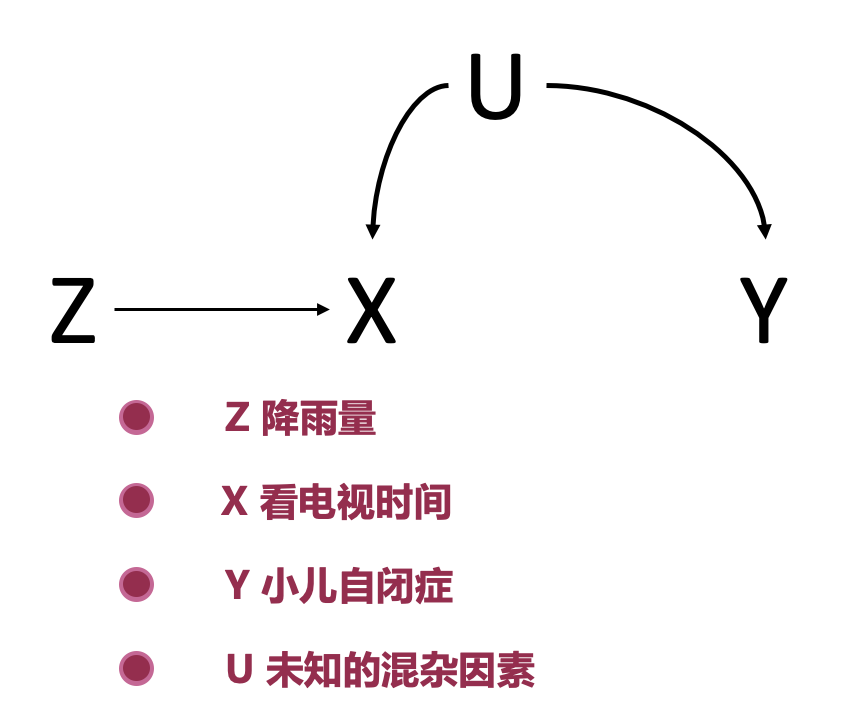
\includegraphics[width=0.42\linewidth,height=\textheight,keepaspectratio]{chapters/images/ch11-image5.png}

\textbf{图11.5 降雨量作为候选工具变量}

\section{工具变量法的分析步骤}\label{ux5de5ux5177ux53d8ux91cfux6cd5ux7684ux5206ux6790ux6b65ux9aa4}

通常采用两阶段的最小二乘法，首先将干预对工具变量做回归，获取干预的预测值，然后将结局对干预的预测值做第二次的回归，所得工具变量估计值为：
两阶段最小二乘的两个阶段应作为一个整体估计，不能把第一阶段的预测值当作普通已观测暴露后再使用常规第二阶段标准误；应采用
IV/2SLS
的联合估计与相应的稳健标准误。估计对象还应在分析前说明是总体效应、依从者效应还是其他局部效应。

\textbf{公式 11.1　Z 为分类变量时的工具变量估计量}

\[
IV = \frac{E\left[Y \middle| Z = 1\right] - E\left[Y \middle| Z = 0\right]}{E\left[X \middle| Z = 1\right] - E\left[X \middle| Z = 0\right]}
\]

Z为分类变量，或：

\textbf{公式 11.2　Z 为连续变量时的工具变量估计量}

\[
IV = \frac{\operatorname{Cov}(Y,Z)}{\operatorname{Cov}(X,Z)}
\]

Z为连续变量

沿用案例9.1中的数据，2016年之前的手术方案大多为显微镜手术，而2016年之后则转变为内镜手术，因此手术的年历时间可能用作工具变量来估算手术方案对疾病缓解的影响。

\begin{tcolorbox}[enhanced jigsaw, arc=.35mm, bottomrule=.15mm, breakable, colback=white, colframe=quarto-callout-note-color-frame, left=2mm, leftrule=.75mm, opacityback=0, rightrule=.15mm, toprule=.15mm]

\vspace{-3mm}\textbf{代码11.1}\vspace{3mm}

\begin{Shaded}
\begin{Highlighting}[]
\KeywordTok{prop}\NormalTok{ Treatment }\KeywordTok{if} \FunctionTok{year}\NormalTok{ \textless{}= 2016}
\KeywordTok{prop}\NormalTok{ Treatment }\KeywordTok{if} \FunctionTok{year}\NormalTok{ \textgreater{} 2016}
\end{Highlighting}
\end{Shaded}

\end{tcolorbox}

\begin{tcolorbox}[enhanced jigsaw, arc=.35mm, bottomrule=.15mm, breakable, colback=white, colframe=quarto-callout-note-color-frame, left=2mm, leftrule=.75mm, opacityback=0, rightrule=.15mm, toprule=.15mm]

\vspace{-3mm}\textbf{代码11.1输出（2016年及以前）}\vspace{3mm}

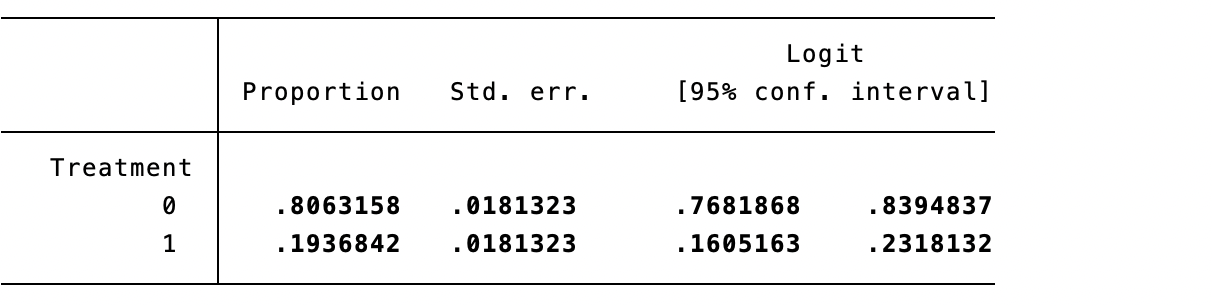
\includegraphics[width=1\linewidth,height=\textheight,keepaspectratio]{chapters/images/ch11-image6.png}

\end{tcolorbox}

\begin{tcolorbox}[enhanced jigsaw, arc=.35mm, bottomrule=.15mm, breakable, colback=white, colframe=quarto-callout-note-color-frame, left=2mm, leftrule=.75mm, opacityback=0, rightrule=.15mm, toprule=.15mm]

\vspace{-3mm}\textbf{代码11.1输出（2017年及以后）}\vspace{3mm}

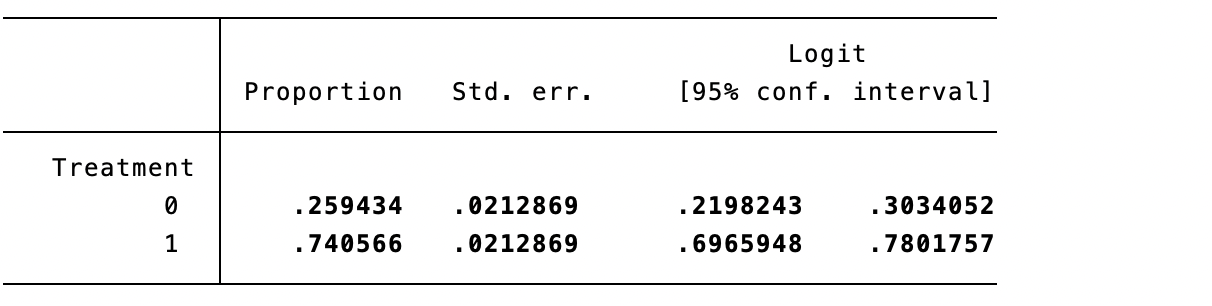
\includegraphics[width=1\linewidth,height=\textheight,keepaspectratio]{chapters/images/ch11-image7.png}

\end{tcolorbox}

2016年以前，显微镜手术的占比是80.6\%，2016年之后，内窥镜手术的占比是74.1\%。因此年历时间与接受何种手术方式存在相关性。

因为感兴趣的结局变量为二分类变量，然而采用逻辑回归进行工具变量分析存在可加性问题。故结局为二分类变量常利用ivprobit命令（即Probit回归，参考第9章），通过两步骤预测替代法进行分类变量结局的工具变量回归。
二分类结局不存在唯一的``标准''IV
模型。ivprobit、两阶段残差纳入法和结构均值模型依赖不同的函数形式与可加性假设；报告时应明确所用模型、效应尺度、第一阶段结果及其识别假设，而不宜将任何一种软件命令视为自动有效。

\begin{tcolorbox}[enhanced jigsaw, arc=.35mm, bottomrule=.15mm, breakable, colback=white, colframe=quarto-callout-note-color-frame, left=2mm, leftrule=.75mm, opacityback=0, rightrule=.15mm, toprule=.15mm]

\vspace{-3mm}\textbf{代码11.2}\vspace{3mm}

\begin{Shaded}
\begin{Highlighting}[]
\KeywordTok{gen}\NormalTok{ year\_iv = (}\FunctionTok{year}\NormalTok{ \textless{}= 2016)}
\KeywordTok{ivprobit}\NormalTok{ Outcome (Treatment = year\_iv)}
\end{Highlighting}
\end{Shaded}

\end{tcolorbox}

\begin{tcolorbox}[enhanced jigsaw, arc=.35mm, bottomrule=.15mm, breakable, colback=white, colframe=quarto-callout-note-color-frame, left=2mm, leftrule=.75mm, opacityback=0, rightrule=.15mm, toprule=.15mm]

\vspace{-3mm}\textbf{代码11.2输出}\vspace{3mm}

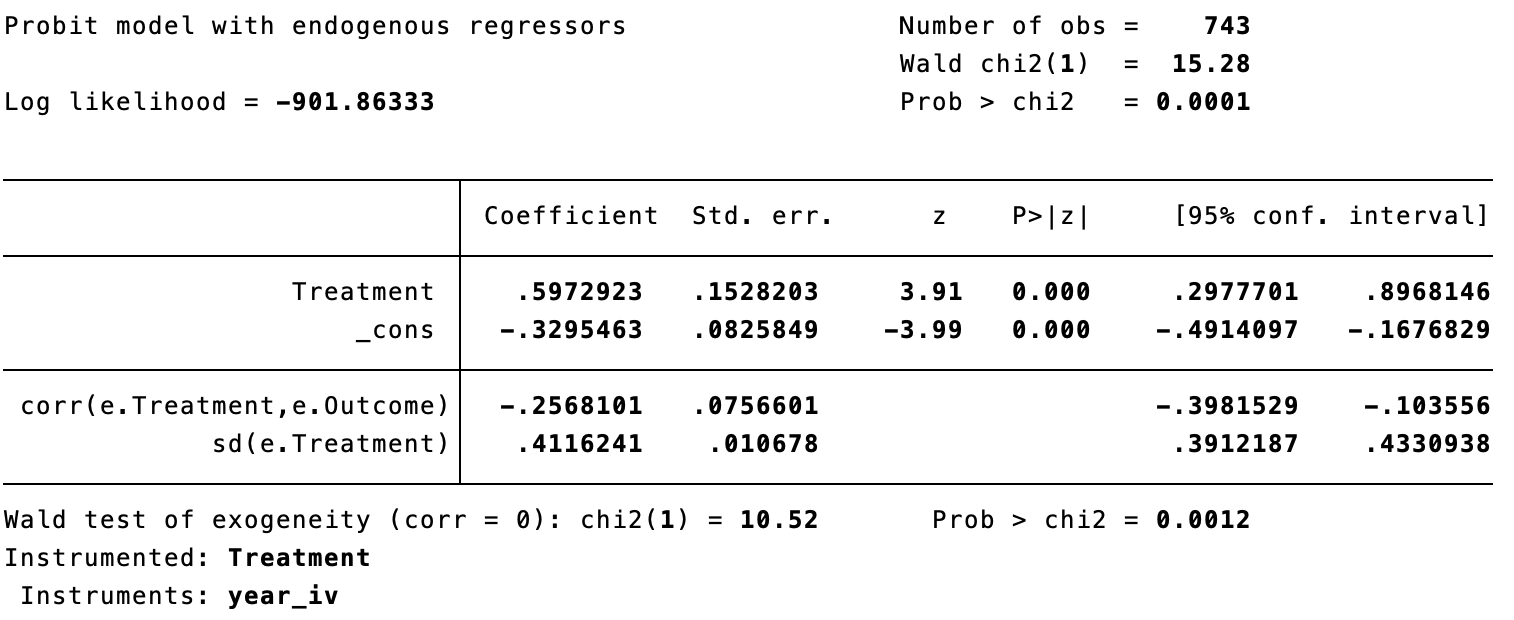
\includegraphics[width=1\linewidth,height=\textheight,keepaspectratio]{chapters/images/ch11-image8.png}

\end{tcolorbox}

模型截距-0.330，表示显微镜组的概率单元值，β1 =
0.597表示内窥镜组与显微镜组的概率单元值差值，内窥镜组的概率单元值为-0.330+0.597=0.267。分别计算累积分布函数值，后代入比值比计算公式得出OR为2.60。同样，此处利用年历时间作为工具变量，需要讨论年历时间可能通过其他医学技术的革新（影像检查的普及导致患者能早期诊断）导致手术效果的提升。
因此，本例的数值结果应理解为在年历时间工具变量及其排除限制可信时的模型估计，而不是对手术方式总体因果效应的无条件证明。

此外，研究手术方式对住院时长的影响，亦可采用工具变量法，此时结局变量为连续变量，可采用两步骤最小二乘法回归。此时回归系数直接表示结局变量的变化幅度，即内窥镜组比显微镜组的住院时长少1.52天。

\begin{tcolorbox}[enhanced jigsaw, arc=.35mm, bottomrule=.15mm, breakable, colback=white, colframe=quarto-callout-note-color-frame, left=2mm, leftrule=.75mm, opacityback=0, rightrule=.15mm, toprule=.15mm]

\vspace{-3mm}\textbf{代码11.3}\vspace{3mm}

\begin{Shaded}
\begin{Highlighting}[]
\NormalTok{ivregress 2sls los (Treatment = year\_iv)}
\end{Highlighting}
\end{Shaded}

\end{tcolorbox}

\begin{tcolorbox}[enhanced jigsaw, arc=.35mm, bottomrule=.15mm, breakable, colback=white, colframe=quarto-callout-note-color-frame, left=2mm, leftrule=.75mm, opacityback=0, rightrule=.15mm, toprule=.15mm]

\vspace{-3mm}\textbf{代码11.3输出}\vspace{3mm}

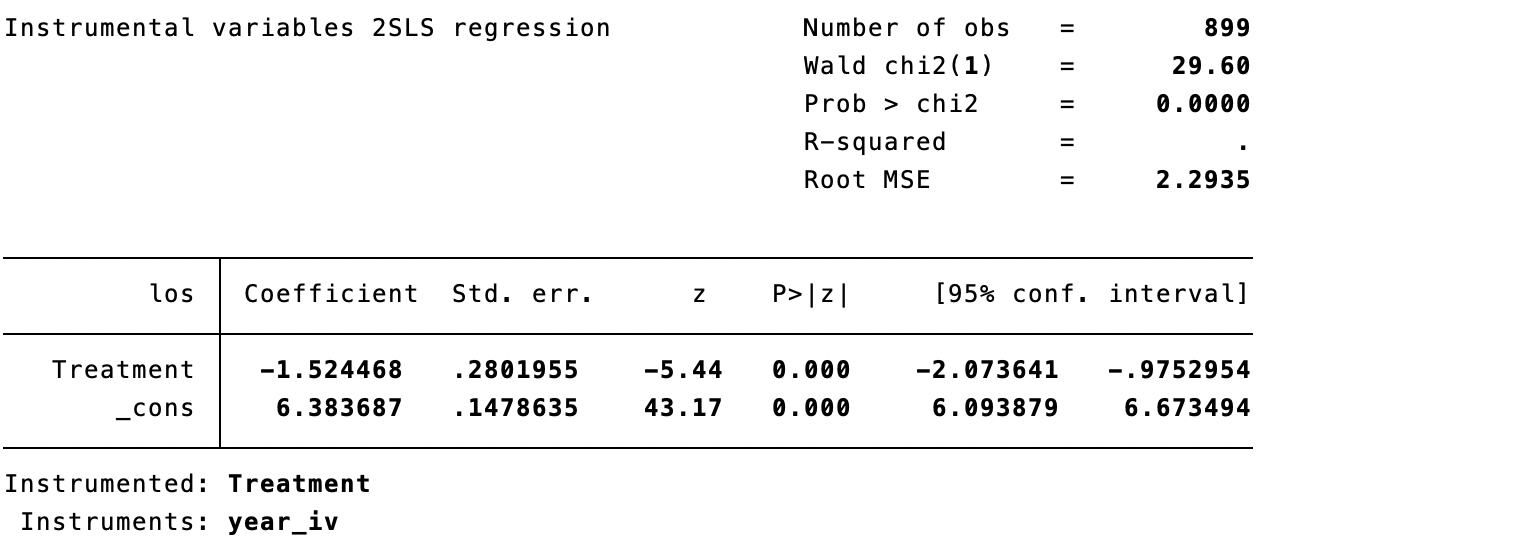
\includegraphics[width=1\linewidth,height=\textheight,keepaspectratio]{chapters/images/ch11-image9.png}

\end{tcolorbox}

\section{工具变量法的统计学检验}\label{ux5de5ux5177ux53d8ux91cfux6cd5ux7684ux7edfux8ba1ux5b66ux68c0ux9a8c}

工具变量的使用受到诸多因素限制，因此需要进行统计学检验与假设：

\begin{enumerate}
\def\labelenumi{\arabic{enumi}.}
\item
  工具变量使用的第一个原则即工具变量与干预相关。工具变量与干预变量的相关性如很小存在弱工具变量问题，弱工具变量会导致因果推断稳定性差。检验弱工具变量的方法：
  弱工具变量会使估计偏向常规回归并造成置信区间失真；应同时报告第一阶段效应、部分
  R²、工具变量数量和弱工具诊断，而不只报告第二阶段 P 值。

  \begin{enumerate}
  \def\labelenumii{\arabic{enumii}.}
  \tightlist
  \item
    第一阶段回归结果中工具变量的显著程度，是否与干预足够相关。
  \item
    第一阶段回归的F值，用来检验工具变量是否显著，如果此检验的F统计量大于10，则可拒绝弱工具变量的原假设（本例F统计量为29.5）。亦可采用Cragg-Donald
    Wald F统计量以及Kleibergen-Paaprk Wald F统计量（可通过Stata
    ivreg2实现）。 F\textgreater10
    是单一内生变量、同方差情形下常见的经验规则，并非普适阈值。在异方差、聚类或多个工具变量时，应优先报告
    Kleibergen-Paap 统计量并参考适用的临界值；必要时采用 Anderson-Rubin
    等对弱工具更稳健的检验与区间。
  \end{enumerate}
\end{enumerate}

\begin{tcolorbox}[enhanced jigsaw, arc=.35mm, bottomrule=.15mm, breakable, colback=white, colframe=quarto-callout-note-color-frame, left=2mm, leftrule=.75mm, opacityback=0, rightrule=.15mm, toprule=.15mm]

\vspace{-3mm}\textbf{代码11.4}\vspace{3mm}

\begin{Shaded}
\begin{Highlighting}[]
\NormalTok{ivreg2 los (Treatment = year\_iv)}
\end{Highlighting}
\end{Shaded}

\end{tcolorbox}

\begin{tcolorbox}[enhanced jigsaw, arc=.35mm, bottomrule=.15mm, breakable, colback=white, colframe=quarto-callout-note-color-frame, left=2mm, leftrule=.75mm, opacityback=0, rightrule=.15mm, toprule=.15mm]

\vspace{-3mm}\textbf{代码11.4输出}\vspace{3mm}

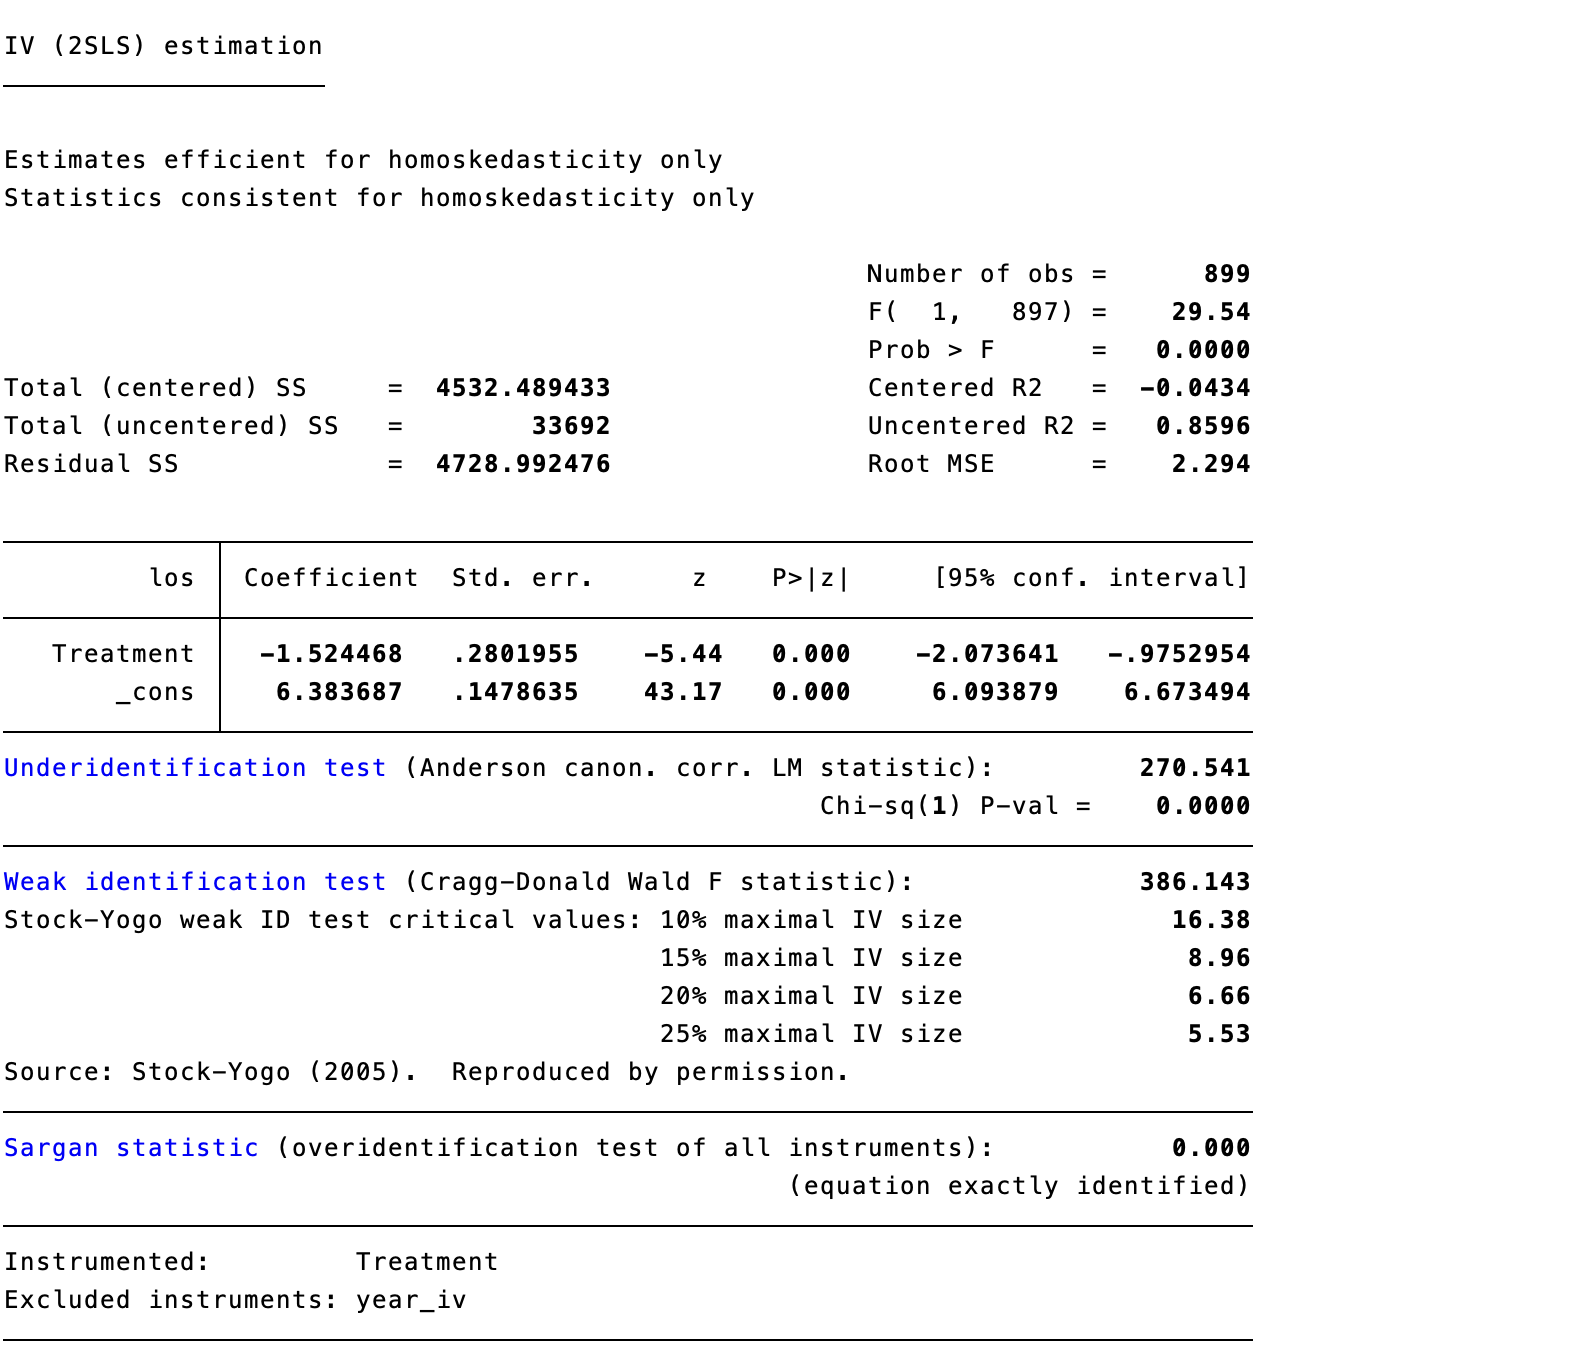
\includegraphics[width=1\linewidth,height=\textheight,keepaspectratio]{chapters/images/ch11-image10.png}

\end{tcolorbox}

\begin{enumerate}
\def\labelenumi{\arabic{enumi}.}
\setcounter{enumi}{1}
\item
  工具变量对结局的影响只能够通过干预，此原则无法通过统计学检验证实，只能通过定性讨论确定，排除其他可能的原因。在案例中年历对疾病缓解的影响可能通过增加内窥镜手术的比例，亦可以通过手术技术的提高，医疗水平的上升等因素，需要分别讨论。研究者所要做的就是找出工具变量影响结局的所有其他可能途径，然后一一反驳。
  排除限制可以被反驳，却不能被数据完全验证。除专家论证外，可报告工具变量与基线协变量的关联、阴性对照结局或暴露、以及针对直接效应的定量敏感性分析；这些检查只能增加或削弱可信度，不能证明假设成立。
\item
  工具变量与结局没有共同的原因，如，可能存在一个L，既导致了年历时间也导致了疾病缓解。本质上也无法检验这个条件，因为可能存在未观察到的工具变量与结局的共同原因，也就无法检验。主要方法都是间接的探讨，主要有两种方法：一种是定性讨论，另一种是过度识别检验。
  过度识别检验只有在工具变量数量多于内生变量时才可进行，且其不显著结果并不证明每一个工具变量有效；若多个工具变量具有相似的违反方式，检验仍可能缺乏识别力。
\item
  此外，工具变量还需要同质性假设，即假设干预对结局的效应在所有的样本中是一致的，即内窥镜的优势在所有个体中是一致的。这个假设通常也是无法证实的，内窥镜的优势可能在侵袭性肿瘤中更大一些，即存在修正效应。在工具变量的研究中，也是无法估算的。
  同质性并非所有 IV
  分析的必要条件。若采用单调性，二元工具变量通常识别的是依从者中的
  LATE；只有在额外的效应同质性或可外推性假设下，才可把该局部效应推广为全体人群的
  ATE。
\end{enumerate}

\section{工具变量的寻觅}\label{ux5de5ux5177ux53d8ux91cfux7684ux5bfbux89c5}

合格的工具变量非常难以寻找。因此，前人对某一类工具变量的使用，在很大程度上对我们今后寻找工具变量能够带来重要启发甚至灵感：严密的逻辑和充分的想象力，是寻找到好的工具变量的必要条件
。

\subsection{来自群体的工具变量}\label{ux6765ux81eaux7fa4ux4f53ux7684ux5de5ux5177ux53d8ux91cf}

个体的干预结局，往往会受到所在集体的某个特征要素的影响。比如，一个人的成绩、收入、社会地位等等，会受到他所在的学校、班级、邻里的特征的影响。为解决这一内生性问题，经济学家和社会学家常常把州、县或大都会地区层面的集聚数据作为学校、班级和邻里等层面解释变量的工具变量。其理由是:
以都会为单位的失业率和贫困率必然和辖区内学校的贫困生比例有关，但又不直接影响学生的怀孕或辍学等行为。

\subsection{来自自然界的工具变量}\label{ux6765ux81eaux81eaux7136ux754cux7684ux5de5ux5177ux53d8ux91cf}

河流、地震、降雨、自然灾害等自然现象在一定地域范围内具有高度的随机，因此可以被假设为与个人和群体的异质性无关，同时，它们又能够影响一些干预过程。例如本章开篇描述的降雨量作为看电视与自闭症的工具变量。

\subsection{来自生理现象的工具变量}\label{ux6765ux81eaux751fux7406ux73b0ux8c61ux7684ux5de5ux5177ux53d8ux91cf}

人类的生老病死既是社会现象，也是生理上的自然现象。出生日期、季度、性别、基因改变等，虽仅仅是有机体的自然历程，但既具有随机性，又往往和特定的经济社会过程相关。饮酒基因型、脂质代谢基因型均可作为干预与冠状动脉综合征结局的工具变量。

\subsection{来自社会空间的工具变量}\label{ux6765ux81eaux793eux4f1aux7a7aux95f4ux7684ux5de5ux5177ux53d8ux91cf}

社会空间的载体，包括具象性的城市、乡村，和非具象性的市场空间等，和人类的行为与结果息息相关，但往往又在特定分析层面上具有独立性、随机性。假设有这样一项研究，一个城市有两家医院提供不同的紧急治疗，位于城市东部的医院专门从事内窥镜手术，西部的医院专门从事显微镜手术。有部分患者将根据家到医院的距离来选择医院，从而选择对应的治疗方法。假设到两家医院的相对距离会影响治疗方法的选择，但是对治疗结局没有直接影响，那么这个相对距离就可以作为工具变量。烟草价格作为研究戒烟与体重增加之间的工具变量。烟草价格高则戒烟概率高，可能会出现体重增加。而烟草价格本身显然和体重没有其他任何的因果逻辑联系。

\section{工具变量的局限性}\label{ux5de5ux5177ux53d8ux91cfux7684ux5c40ux9650ux6027}

第一，找到好的工具变量非常之难。它难寻的原因，恰恰就是它的力量所在:
因为它必须永远置身模型之外。当我们一心关注模型本身之时，注意力自然只会放在模型之内。因此，只要我们变换思维的角度，开始习惯从模型之外寻找解决问题的武器，多从前人巧妙使用工具变量的实例里获得启发，我们就会发现，工具变量虽然难寻，但绝非了无痕迹。

第二，工具变量对于模型不存在未观察的混杂因素无法用统计方法检验的。这一尴尬直接导致的结果就是:
不管熟悉还是不熟悉工具变量方法的读者，面对一篇工具变量分析的论文，其第一反应总是首先质疑其合法性。但凭心而论，和其他一些解决混杂因素的常用模型相比，工具变量分析承受了过多的挑刺和压力。当倾向值匹配模型假设一切偏误都来自可观察的变量，读者们往往能不假思索地接受这些武断的假设。

第三，工具变量估计量往往因工具变量的选取而异，工具变量对样本的影响，往往是非均质的，所以工具变量估计量带有权重性的特征，即局部干预效应。案例中存在一部分患者无论什么年份都会接受内窥镜手术或显微镜手术（比如，某个医生只会一种手术方式），另一部分患者如果在不同年份去医院可能接受不同的手术方式。因此，从工具变量分析里得到的结论，往往只适用于后面那部分患者。不过，与其说这是工具变量方法的不足，倒不如说是一种优势，使样本变得更加具有目标性，结论也更有说服力。
报告时应说明依从者在临床上的含义及其与总体样本的差异；LATE
具有明确目标人群，但不应被不加说明地外推给从不接受或总是接受某种治疗的患者。

第四，工具变量的使用看似难以举一反三，但哪怕是前人使用过的失败的工具变量，都可能具有借鉴和推广意义。案例中以2016年作为分界线，只在单个中心有效，而在其他中心情况就会大有不同。

\section{孟德尔随机化}\label{ux5b5fux5fb7ux5c14ux968fux673aux5316}

孟德尔随机化（Mendelian
randomization，MR）是在观察性数据中使用遗传变异来估计暴露和结局之间的因果关系。暴露可以是生物标志物、人体测量指标或任何其他可能影响结果的风险因素。通常情况下，结局是疾病。之所以称为随机化，是因为基因的形成过程是随机的，随机化的结果形成一种基因型和另一种基因型，从而产生不同的表型。

孟德尔随机化也是一种工具变量法，同样需要满足工具变量的三个假设。基因型要与基因型的表达产物相关，即所感兴趣的干预、生物标志物或者其他风险因素；基因型对结局的影响只能通过此表达产物传递；基因型与结局之间，没有共同的原因。
对 MR
而言，第三项独立性假设还要求控制或评估祖源结构、遗传连锁和家系效应；排除限制则要求警惕横向多效性。垂直多效性若完全位于暴露的下游，通常不违反
IV 假设；横向多效性则会造成偏倚。

\subsection{案例11.1}\label{ux6848ux4f8b11.1}

研究者感兴趣低密度脂蛋白（LDL）与冠脉综合症之间的关系，X 即 LDL，Y
为冠脉综合症，Z 为工具变量为引入的与 LDL
相关的基因型，如单核苷酸多态性（SNPs）。工具变量三个统计学假设中（图11.1），第一点可以被证实，只需计算基因型与LDL的相关性，而第二，第三点是不可证实的，需经过讨论。单个基因型的效应可能有很多，基因型对结局的影响，可能不通过所感兴趣的路径。单核苷酸多态性可以影响LDL的水平高低，亦或影响胆固醇水平高低。基因型与结局之间没有共同原因也无法证实。基因型可能和其他的基因位点形成遗传不平衡，导致多个基因形成遗传连锁，而其他基因型可能和结局相关；亦可能存在某个人群，该人群中基因型的某个等位基因出现高频突变，并且该人群中冠脉综合征发生风险比较低。

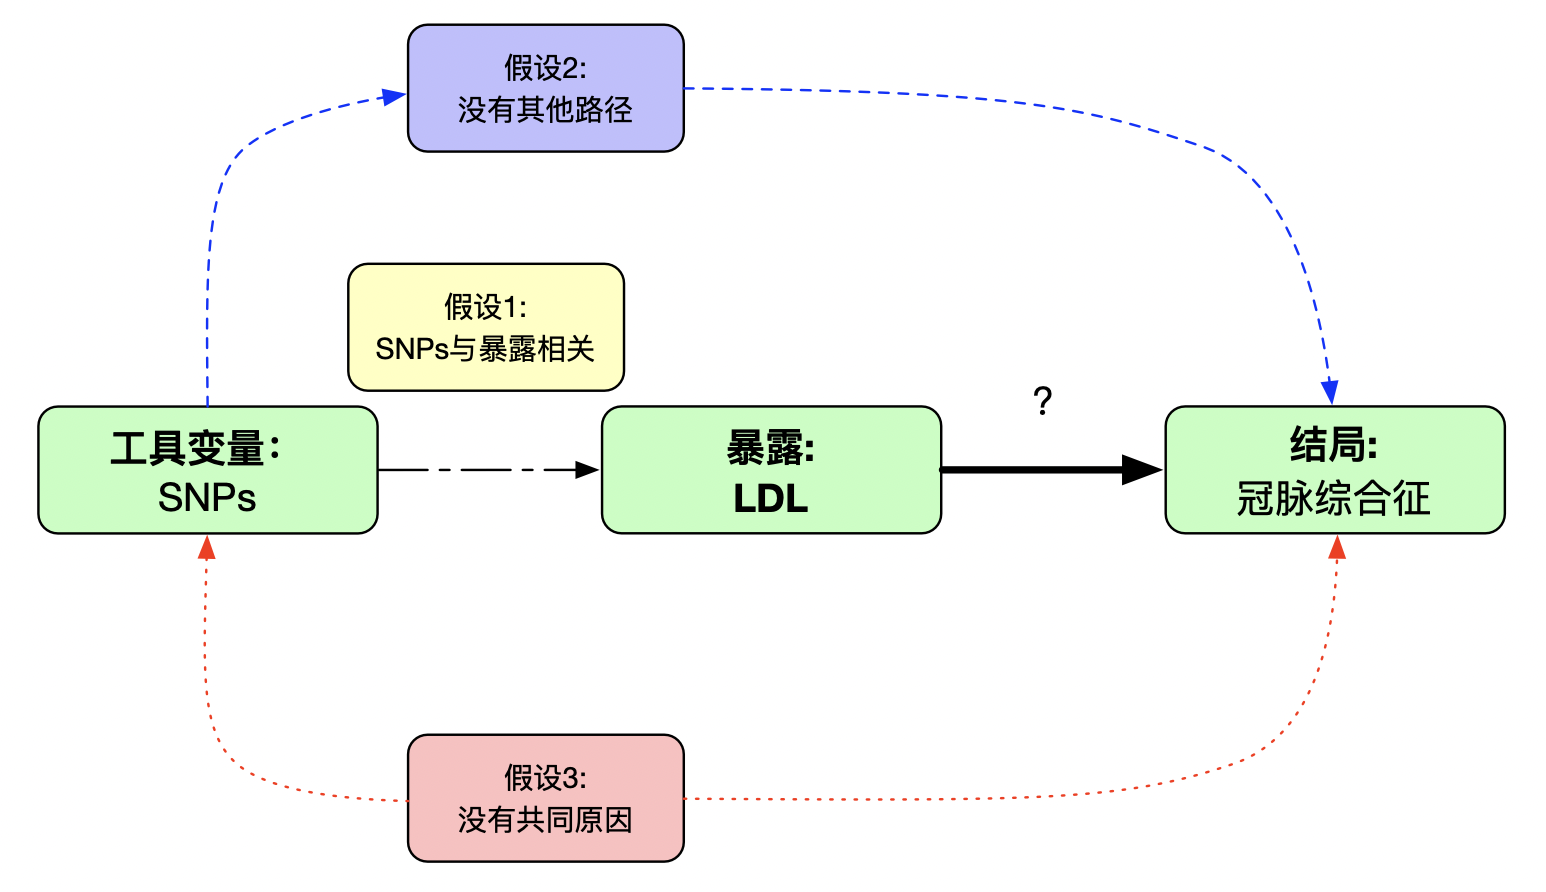
\includegraphics[width=1\linewidth,height=\textheight,keepaspectratio]{chapters/images/ch11-image11.png}

\textbf{图11.6 孟德尔随机化的假设}

孟德尔随机化的研究方法大致有两种：

\textbf{独立样本MR：}该方法利用单一研究样本，通过使用两阶段最小二乘法回归模型，定量估计暴露因素与结局之间的关联效应大小。由于该方法局限于单个样本，把握度较小，工具变量的选择也比较局限，容易受到潜在混杂因素的影响。

\textbf{两样本MR：}基因型与暴露、基因型与结局的关联研究人群来自相同人群的两个独立样本，要求两样本具有相似的年龄、性别和种族分布特征。因为样本量较大，该方法可以获得更大的把握度。两样本MR因为全球大量全基因组关联分析（GWAS）合作组的公共数据而被广泛使用。
两样本 MR 还应说明样本重叠程度、祖源可比性、暴露和结局 GWAS
的测量定义及选择机制。样本重叠在弱工具存在时可使两样本估计向观察性关联偏移。

两样本MR的研究步骤分为四步：

\begin{enumerate}
\def\labelenumi{\arabic{enumi}.}
\tightlist
\item
  在GWAS数据库（https://www.ebi.ac.uk/gwas/）中寻找与研究干预相关的SNPs，获得一系列的已经发表的文章以及文章中的SNPs数据，查询这些SNPs的p值来筛选对应的SNPs（\textless{}
  10-8），剔除有遗传不平衡的SNPs，记录回归系数和标准差。
  常用的全基因组显著性起点是
  P\textless5×10⁻⁸；随后通常进行连锁不平衡剔除（clumping）、等位基因协调（harmonization）和工具强度评估。阈值与
  LD 参数应预先报告，并结合所研究性状的遗传结构解释。
\item
  在数据库中输入结局，查询上述筛选出的SNPs与结局变量的相关性（回归系数和标准差）。
\item
  估算因果效应方法，一般采取逆方差加权法，中位数法和Egger法。
  主分析应预先指定；加权中位数、MR-Egger、加权模式、异质性检验、留一法和
  MR-PRESSO
  等应作为对不同多效性假设的敏感性分析，而非只挑选产生显著结果的方法。
\item
  由于往往暴露会与多个SNPs存在相关性，即存在多个工具变量，需要合并多个SNPs的估算。孟德尔随机化的整合效应图中，点和十字是每一个SNP作为工具变量估算的干预与结局的关系，拟合所有的SNP绘制出了一条斜线，其斜率就是LDL对冠脉综合症发生的风险。
\end{enumerate}

\textbf{案例11.1数据表}

{\def\LTcaptype{none} % do not increment counter
\begin{longtable}[]{@{}crrrrrr@{}}
\toprule\noalign{}
rsid & ldlcbeta & ldlcse & ldlcp2 & acsbeta & acsse & acsp2 \\
\midrule\noalign{}
\endhead
\bottomrule\noalign{}
\endlastfoot
rs1010167 & -0.025 & 0.0039 & 3.00E-10 & -0.028 & 0.01897 & 0.14 \\
rs10102164 & 0.032 & 0.0045 & 3.00E-12 & 0.012 & 0.01661 & 0.47 \\
rs10401969 & 0.12 & 0.0073 & 2.00E-60 & 0.11 & 0.02958 & 0.0002 \\
rs10790162 & 0.076 & 0.0071 & 3.00E-26 & 0.13 & 0.02735 & 2.00E-06 \\
rs10832962 & 0.032 & 0.0040 & 2.00E-15 & 0.044 & 0.01564 & 0.0049 \\
rs10903129 & -0.033 & 0.0036 & 4.00E-19 & -0.012 & 0.01367 & 0.38 \\
\ldots{} & \ldots{} & \ldots{} & \ldots{} & \ldots{} & \ldots{} &
\ldots{} \\
\end{longtable}
}

数据格式如上，每一行为一个工具变量（基因位点rsid标识），ldlcbeta、ldlcse、ldlcp2分别代表该基因位点与LDL的相关系数，标准差以及p值；而acsbeta、acsse、acsp2分别代表该基因位点与结局事件冠脉综合征的相关系数，标准差以及p值。这些数据来源于两个大型GWAS研究，即LDL的GWAS和冠脉综合征的GWAS研究。

\begin{tcolorbox}[enhanced jigsaw, arc=.35mm, bottomrule=.15mm, breakable, colback=white, colframe=quarto-callout-note-color-frame, left=2mm, leftrule=.75mm, opacityback=0, rightrule=.15mm, toprule=.15mm]

\vspace{-3mm}\textbf{代码11.5}\vspace{3mm}

\begin{Shaded}
\begin{Highlighting}[]
\NormalTok{mregger acsbeta ldlcbeta [aw=1/(acsse\^{}2)], ivw }\KeywordTok{fe}
\KeywordTok{lincom}\NormalTok{ ldlcbeta, }\KeywordTok{or}
\end{Highlighting}
\end{Shaded}

\end{tcolorbox}

\begin{tcolorbox}[enhanced jigsaw, arc=.35mm, bottomrule=.15mm, breakable, colback=white, colframe=quarto-callout-note-color-frame, left=2mm, leftrule=.75mm, opacityback=0, rightrule=.15mm, toprule=.15mm]

\vspace{-3mm}\textbf{代码11.5输出}\vspace{3mm}

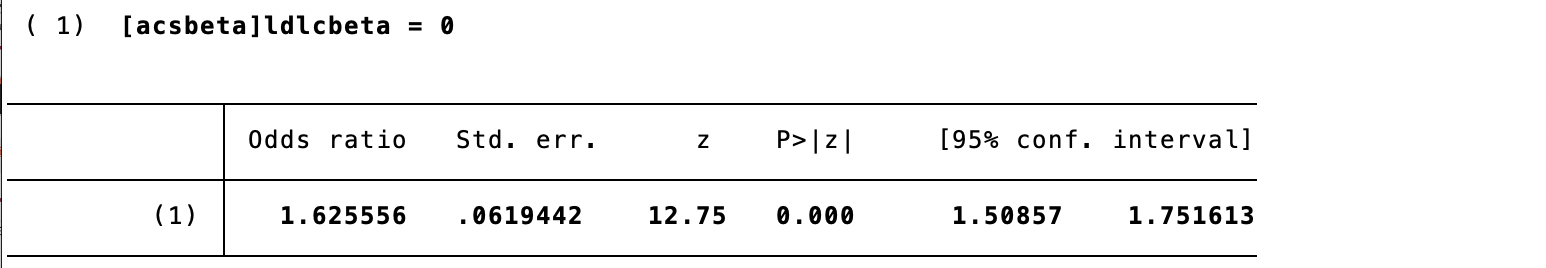
\includegraphics[width=1\linewidth,height=\textheight,keepaspectratio]{chapters/images/ch11-image12.png}

\end{tcolorbox}

结果表明采取逆方差加权法合并多个SNPs分析得出1个单位LDL的增加会导致冠脉综合征风险增加1.63倍。

\begin{tcolorbox}[enhanced jigsaw, arc=.35mm, bottomrule=.15mm, breakable, colback=white, colframe=quarto-callout-note-color-frame, left=2mm, leftrule=.75mm, opacityback=0, rightrule=.15mm, toprule=.15mm]

\vspace{-3mm}\textbf{代码11.6}\vspace{3mm}

\begin{Shaded}
\begin{Highlighting}[]
\NormalTok{mrmedian acsbeta acsse ldlcbeta ldlcse, weighted}
\KeywordTok{lincom}\NormalTok{ beta, }\KeywordTok{or}
\end{Highlighting}
\end{Shaded}

\end{tcolorbox}

\begin{tcolorbox}[enhanced jigsaw, arc=.35mm, bottomrule=.15mm, breakable, colback=white, colframe=quarto-callout-note-color-frame, left=2mm, leftrule=.75mm, opacityback=0, rightrule=.15mm, toprule=.15mm]

\vspace{-3mm}\textbf{代码11.6输出}\vspace{3mm}

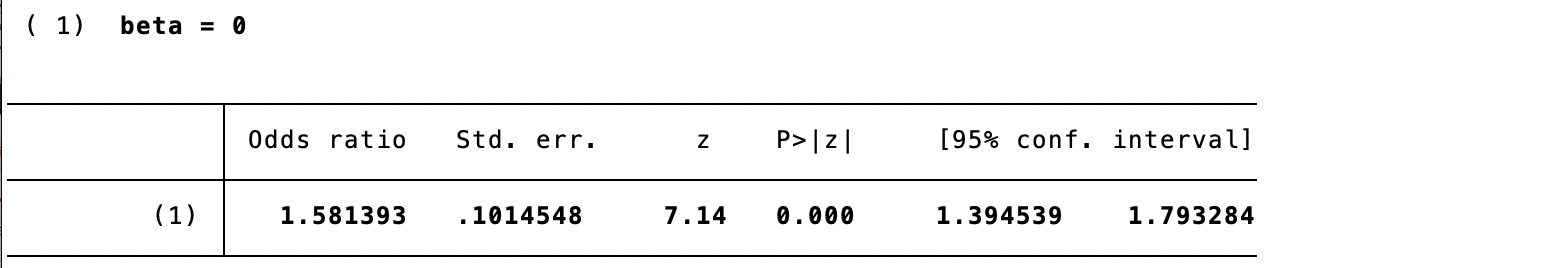
\includegraphics[width=1\linewidth,height=\textheight,keepaspectratio]{chapters/images/ch11-image13.png}

\end{tcolorbox}

\begin{tcolorbox}[enhanced jigsaw, arc=.35mm, bottomrule=.15mm, breakable, colback=white, colframe=quarto-callout-note-color-frame, left=2mm, leftrule=.75mm, opacityback=0, rightrule=.15mm, toprule=.15mm]

\vspace{-3mm}\textbf{代码11.7}\vspace{3mm}

\begin{Shaded}
\begin{Highlighting}[]
\NormalTok{mregger acsbeta ldlcbeta [aw=1/(acsse\^{}2)]}
\KeywordTok{lincom}\NormalTok{ slope, }\KeywordTok{or}
\end{Highlighting}
\end{Shaded}

\end{tcolorbox}

\begin{tcolorbox}[enhanced jigsaw, arc=.35mm, bottomrule=.15mm, breakable, colback=white, colframe=quarto-callout-note-color-frame, left=2mm, leftrule=.75mm, opacityback=0, rightrule=.15mm, toprule=.15mm]

\vspace{-3mm}\textbf{代码11.7输出}\vspace{3mm}

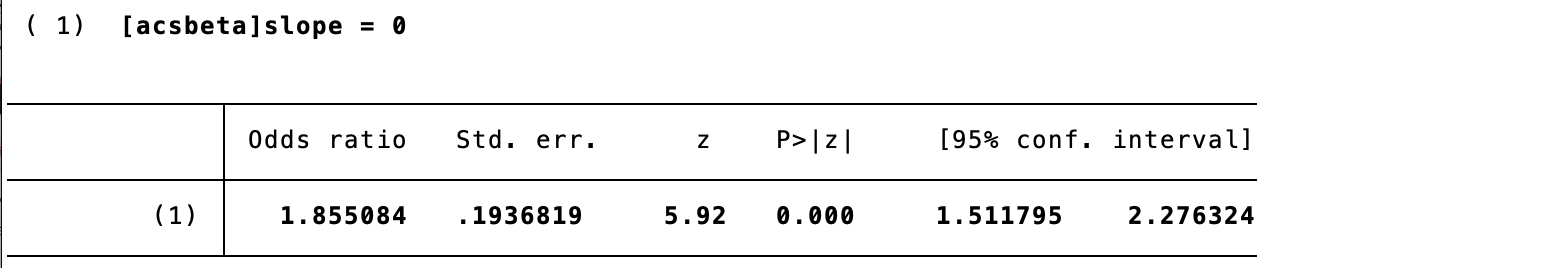
\includegraphics[width=1\linewidth,height=\textheight,keepaspectratio]{chapters/images/ch11-image14.png}

\end{tcolorbox}

几种方法得出的结论基本一致。亦可以绘制出整合效应图和森林图。整合效应图上每一个十字星代表一个SNP作为工具变量，拟合的直线及其95\%置信区间的斜率即代表效应大小。森林图的解读与荟萃分析一致，每个SNP类似荟萃分析中的一项研究。
图形与各 SNP
的效应估计应同时报告置信区间、异质性指标和离群变异的处理规则；不同 MR
方法结果一致只能提供支持性证据，不能替代对工具变量假设的论证。

\begin{tcolorbox}[enhanced jigsaw, arc=.35mm, bottomrule=.15mm, breakable, colback=white, colframe=quarto-callout-note-color-frame, left=2mm, leftrule=.75mm, opacityback=0, rightrule=.15mm, toprule=.15mm]

\vspace{-3mm}\textbf{代码11.8}\vspace{3mm}

\begin{Shaded}
\begin{Highlighting}[]
\NormalTok{mreggerplot acsbeta acsse ldlcbeta ldlcse, gpci}
\NormalTok{mrforest acsbeta acsse ldlcbeta ldlcse, ivid(rsid) models(4)}
\end{Highlighting}
\end{Shaded}

\end{tcolorbox}

\begin{tcolorbox}[enhanced jigsaw, arc=.35mm, bottomrule=.15mm, breakable, colback=white, colframe=quarto-callout-note-color-frame, left=2mm, leftrule=.75mm, opacityback=0, rightrule=.15mm, toprule=.15mm]

\vspace{-3mm}\textbf{代码11.8输出（整合效应图）}\vspace{3mm}

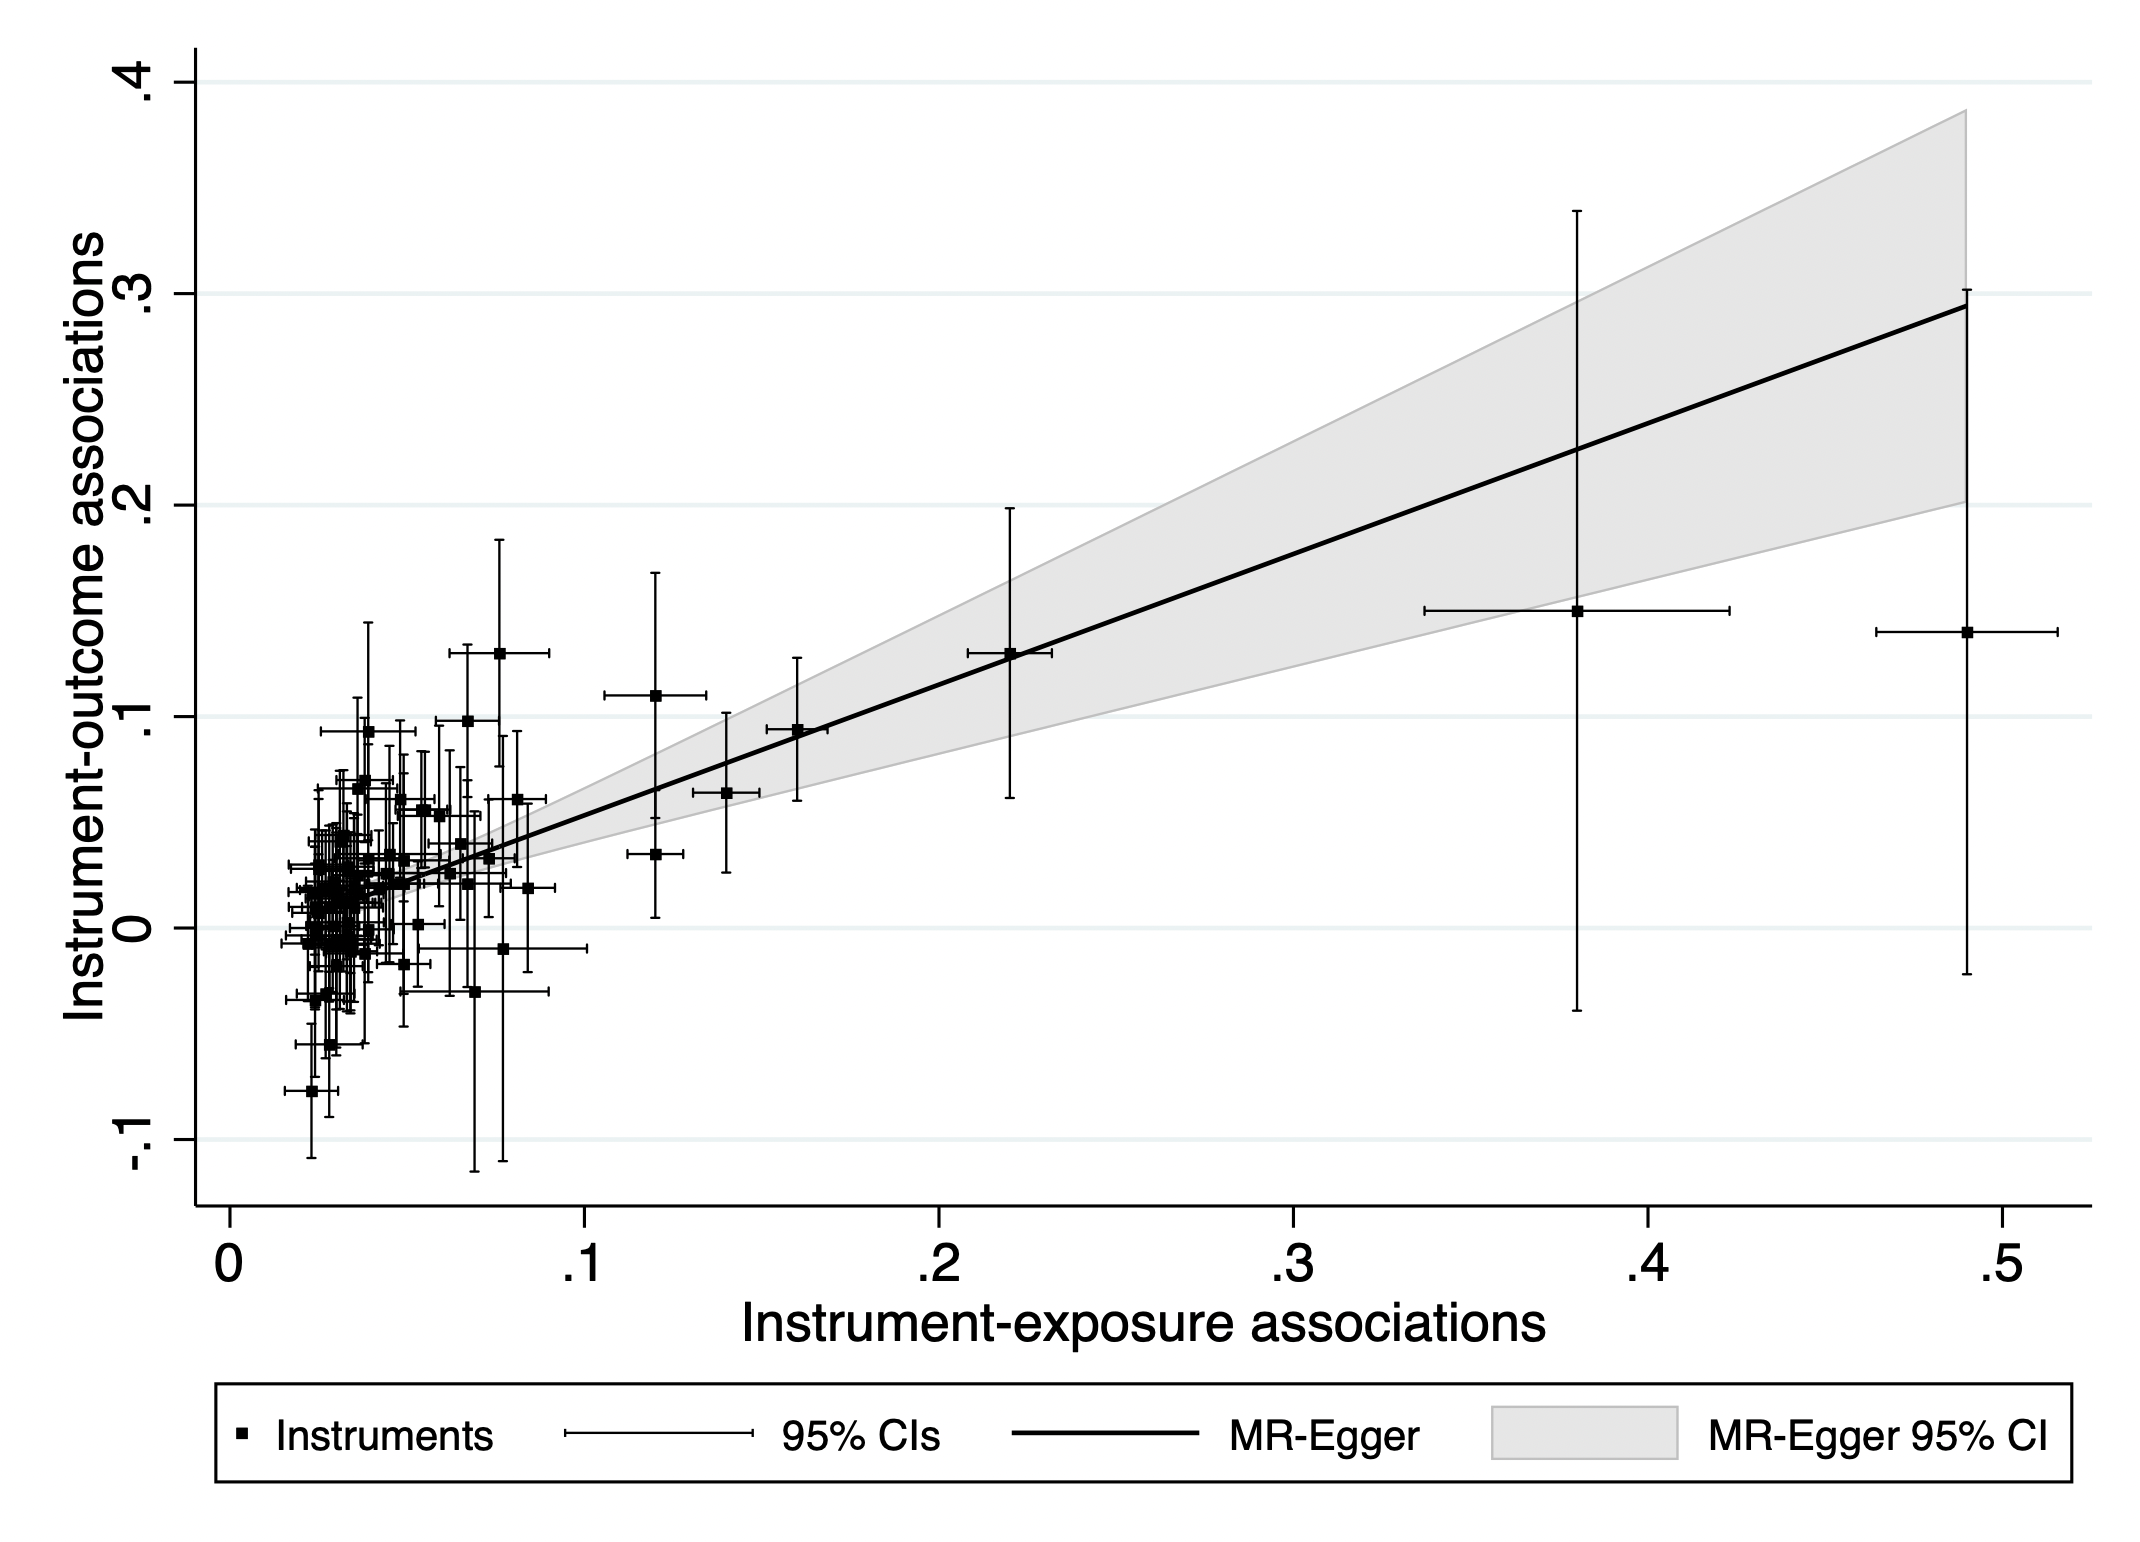
\includegraphics[width=1\linewidth,height=\textheight,keepaspectratio]{chapters/images/ch11-image15.png}

\end{tcolorbox}

\begin{tcolorbox}[enhanced jigsaw, arc=.35mm, bottomrule=.15mm, breakable, colback=white, colframe=quarto-callout-note-color-frame, left=2mm, leftrule=.75mm, opacityback=0, rightrule=.15mm, toprule=.15mm]

\vspace{-3mm}\textbf{代码11.8输出（森林图）}\vspace{3mm}

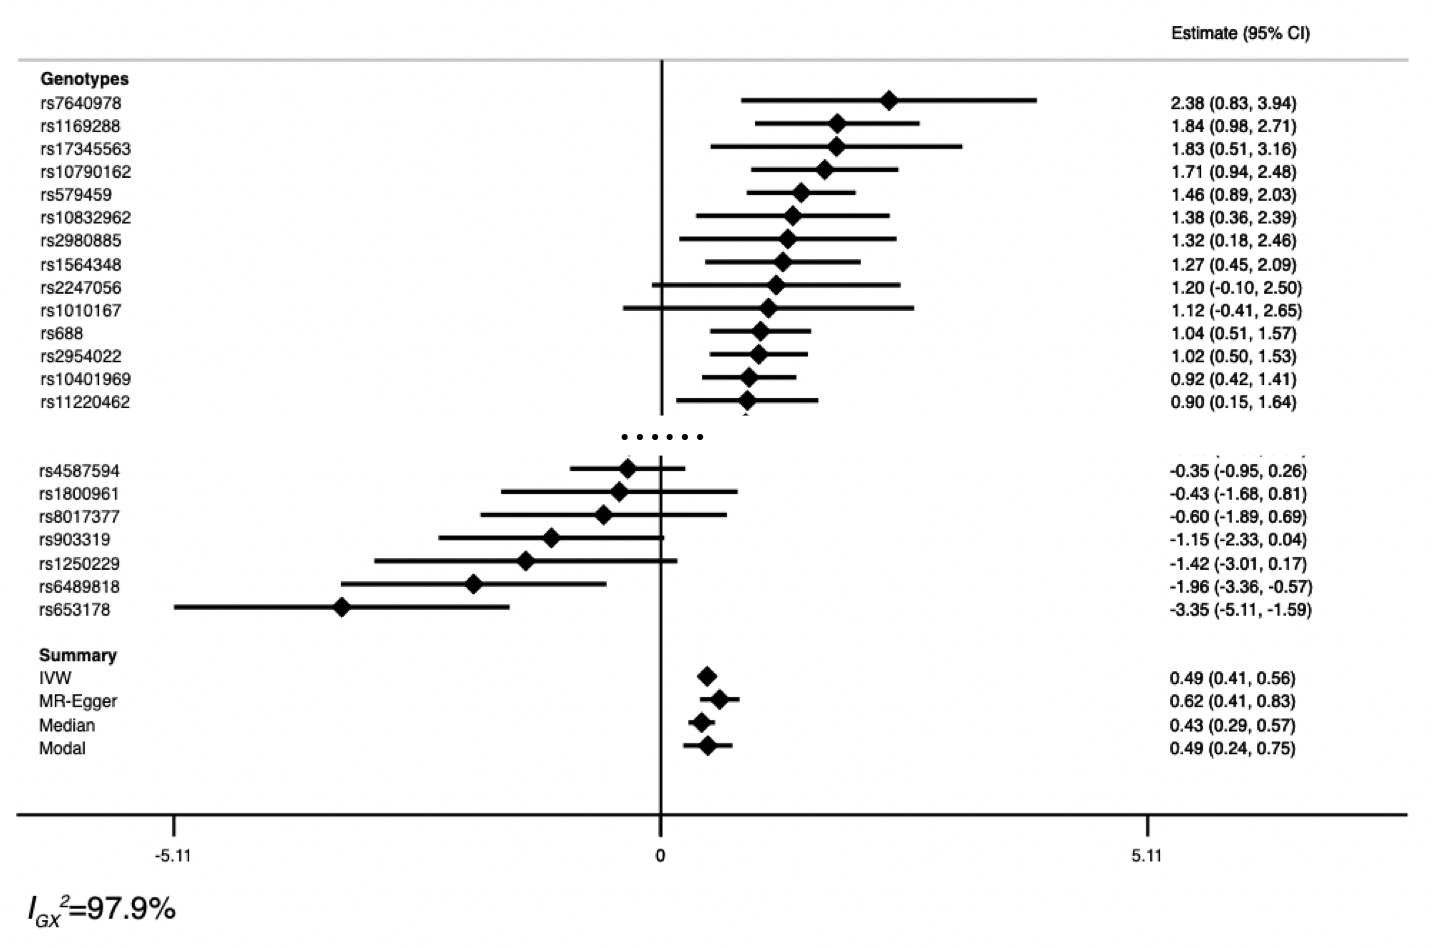
\includegraphics[width=1\linewidth,height=\textheight,keepaspectratio]{chapters/images/ch11-image16.png}

\end{tcolorbox}

虽然MR应用广泛，需了解其优势和局限性。 MR 研究的报告可参考 STROBE-MR
声明：明确因果问题和 estimand，描述数据来源、SNP 选择和协调、三项 IV
假设的依据、主分析与敏感性分析、数据/代码可得性及外推边界（Skrivankova
等，2021）。

MR的优点是一个天然的随机化过程，没有反向的因果。当暴露与结果之间的关联不是由于暴露导致结果变化，而是由于结果导致暴露变化时，则发生反向因果关系。由于个体的基因型是在受孕时确定的，无法更改，因此不会存在因果关系与基因型相关联的反向因果关系，这也是孟德尔随机化的优势。

在某些情况下，许多感兴趣的风险无法可靠地衡量，亦或无法通过随机化方法实现干预，如腰围，体重等。在这种情况下，可以将遗传变异用作暴露的代理，并且可以追溯这些风险与结果的关联。

此外，工具变量估计值不会因暴露中的经典测量误差（包括个体内部差异）而衰减。这与观察性研究相反，在观察性研究中，暴露中的测量误差通常会导致回归系数朝着零值的方向衰减。

当然MR也存在诸多缺点，难以找到合适的SNPs，需要大样本的GWAS研究；单个SNP是一个弱工具，因此需要很多SNPs集合构成一个综合因果估计；MR为工具变量方法，统计学假设中需要考虑第二第三原则违反情况下的因果推断，可以通过估计工具变量和各种特征之间的关系来分析讨论，虽然这些评估不能证明这两个假设的成立，但可以提供有关其合理性的证据；MR无法解释生物学机制，发育过程中的一些代偿可能会导致表型的改变，表型也可能是多样性的。
尤其应避免把 MR 结果称为``天然随机试验的证明''。MR
估计反映遗传预测的、通常是长期的暴露差异；它未必等同于在特定年龄、剂量和持续时间实施临床干预所产生的效果。

\section{附录：孟德尔随机化研究的关键评估清单}\label{ux9644ux5f55ux5b5fux5fb7ux5c14ux968fux673aux5316ux7814ux7a76ux7684ux5173ux952eux8bc4ux4f30ux6e05ux5355}

\subsection{孟德尔随机化的核心假设}\label{ux5b5fux5fb7ux5c14ux968fux673aux5316ux7684ux6838ux5fc3ux5047ux8bbe}

\begin{itemize}
\tightlist
\item
  是否有足够的证据表明遗传变异与所关注的风险因素密切相关？
\item
  遗传变异是否与潜在的混杂因素有关？是否介绍了这种关系？
\item
  遗传变异是否有办法通过其他途径影响结果（横向多变性）？是否介绍了多种孟德尔随机化方法（如MR
  Egger、中位数和模式估计，或使用阴性对照人群），以更全面地调查这一问题？
\end{itemize}

\subsection{方法报告}\label{ux65b9ux6cd5ux62a5ux544a}

\begin{itemize}
\tightlist
\item
  暴露和结果的效应和其他等位基因的编码方向是否相同？
\item
  两样本的研究：两个样本是否取自同一人群？
\item
  两样本是否独立？
\item
  分析是否只限于独立的工具变量（即删除了遗传连锁不平衡的SNPs）或分析是否允许工具变量之间的相关性？
\end{itemize}

\subsection{数据展示}\label{ux6570ux636eux5c55ux793a}

\begin{itemize}
\tightlist
\item
  是否将结果表述为遗传关联、工具变量估计，或两者都是？
\item
  如果提供的是工具变量估计值，是否将其与传统的观察性估计值进行了比较？
\item
  是否提供敏感性分析，如MR
  Egger、加权中位数和模式孟德尔随机化，或使用阴性对照人群？
\item
  是否手动挑选哪些SNPs进入工具变量以解决多态性问题？如果是这样，其方法和理由是否清楚？
\item
  是否在补充材料中提供了使用的数据（特别是在群体水平上进行的孟德尔随机化分析），以便研究人员复制他们的发现？
\end{itemize}

\subsection{解释}\label{ux89e3ux91ca}

\begin{itemize}
\tightlist
\item
  如果孟德尔随机化估计值与观察估计值相似，并提供了支持因果效应的证据，是否是由于单一研究中的弱工具偏倚或通过横向多态性的混杂造成的？
\item
  如果孟德尔随机化估计值与观察性估计值不同，并提供了因果效应的少量证据，是否是由于使用了弱工具造成的偏差或由于多态性造成的负向混杂？
\item
  孟德尔随机化提供了风险因素在群体一生中的影响估计，对特定年龄段的干预措施有同样大小的效果吗？
\item
  孟德尔随机化估计的95\%置信区间是否足够精确，因果效应是否临床意义的差异？
\end{itemize}

\subsection{临床意义}\label{ux4e34ux5e8aux610fux4e49}

\begin{itemize}
\tightlist
\item
  结果是否与其他形式的证据相互印证？能否像PCSK9抑制剂那样进行临床试验以提供明确的证据？
\item
  如果随机临床试验不可行（如饮酒和心脏病风险的情况）或不可能在短期内进行（如降低BMI和心脏病风险的生活方式干预的情况），并且现有的证据来自多个孟德尔随机化研究和其他稳健的研究设计，趋向于一个类似的结果，并显示出关联的一致性，这些信息可以用来指导病人护理；例如，建议减肥以预防心脏病，或建议不要适度饮酒以预防心血管疾病。
  在用于临床建议前，还应结合干预试验、机制研究、观察性研究和不同人群中的
  MR
  结果进行证据三角验证，并清楚区分遗传预测的终生暴露效应与可操作的短期干预效应。
\end{itemize}

\section{本章参考文献}\label{ux672cux7ae0ux53c2ux8003ux6587ux732e}

\begin{enumerate}
\def\labelenumi{\arabic{enumi}.}
\tightlist
\item
  Hernán MA, Robins JM. Instruments for causal inference: an
  epidemiologist's dream? \emph{Epidemiology}. 2006;17:360--372.
  \href{https://pubmed.ncbi.nlm.nih.gov/16755261/}{PMID: 16755261}
\item
  Baiocchi M, Cheng J, Small DS. Instrumental variable methods for
  causal inference. \emph{Statistics in Medicine}. 2014;33:2297--2340.
  \href{https://pubmed.ncbi.nlm.nih.gov/24599889/}{PMID: 24599889}
\item
  Lousdal ML. An introduction to instrumental variable assumptions,
  validation and estimation. \emph{Emerging Themes in Epidemiology}.
  2018;15:1. \href{https://pubmed.ncbi.nlm.nih.gov/29387137/}{PMID:
  29387137}
\item
  Garabedian LF, Chu P, Toh S, et al.~Potential bias of instrumental
  variable analyses for observational comparative effectiveness
  research. \emph{Annals of Internal Medicine}. 2014;161:131--138.
  \href{https://pubmed.ncbi.nlm.nih.gov/25023252/}{PMID: 25023252}
\item
  Bowden J, Davey Smith G, Burgess S. Mendelian randomization with
  invalid instruments: effect estimation and bias detection through
  Egger regression. \emph{International Journal of Epidemiology}.
  2015;44:512--525.
  \href{https://pubmed.ncbi.nlm.nih.gov/26050253/}{PMID: 26050253}
\item
  Bowden J, Davey Smith G, Haycock PC, Burgess S. Consistent estimation
  in Mendelian randomization with some invalid instruments using a
  weighted median estimator. \emph{Genetic Epidemiology}.
  2016;40:304--314.
  \href{https://pubmed.ncbi.nlm.nih.gov/27061298/}{PMID: 27061298}
\item
  Burgess S, Davey Smith G, Davies NM, et al.~Guidelines for performing
  Mendelian randomization investigations. \emph{Wellcome Open Research}.
  2020;4:186. \href{https://pubmed.ncbi.nlm.nih.gov/32760811/}{PMID:
  32760811}
\item
  Skrivankova VW, Richmond RC, Woolf BAR, et al.~Strengthening the
  Reporting of Observational Studies in Epidemiology Using Mendelian
  Randomization: The STROBE-MR Statement. \emph{JAMA}.
  2021;326:1614--1621.
  \href{https://pubmed.ncbi.nlm.nih.gov/34698778/}{PMID: 34698778}
\end{enumerate}

\bookmarksetup{startatroot}

\chapter{断点回归}\label{ux65adux70b9ux56deux5f52}

\begin{tcolorbox}[enhanced jigsaw, arc=.35mm, bottomrule=.15mm, bottomtitle=1mm, breakable, colback=white, colbacktitle=quarto-callout-note-color!10!white, colframe=quarto-callout-note-color-frame, coltitle=black, left=2mm, leftrule=.75mm, opacityback=0, opacitybacktitle=0.6, rightrule=.15mm, title=\textcolor{quarto-callout-note-color}{\faInfo}\hspace{0.5em}{编写说明}, titlerule=0mm, toprule=.15mm, toptitle=1mm]

本章内容整理中。可将已校订的 Word 书稿（\texttt{乔Book/}
目录）正文迁移至此，公式用 \texttt{\$...\$} /
\texttt{\$\$...\$\$}，图片放 \texttt{images/}，代码用
\texttt{\{r\}\ 或}\{python\} 代码块。

\end{tcolorbox}

\section{精确断点与模糊断点}\label{ux7cbeux786eux65adux70b9ux4e0eux6a21ux7ccaux65adux70b9}

\emph{待补充。}

\section{控制变量断点的识别}\label{ux63a7ux5236ux53d8ux91cfux65adux70b9ux7684ux8bc6ux522b}

\emph{待补充。}

\section{断点回归估计方法}\label{ux65adux70b9ux56deux5f52ux4f30ux8ba1ux65b9ux6cd5}

\emph{待补充。}

\section{断点有效性检验}\label{ux65adux70b9ux6709ux6548ux6027ux68c0ux9a8c}

\emph{待补充。}

\section{断点回归的应用}\label{ux65adux70b9ux56deux5f52ux7684ux5e94ux7528}

\emph{待补充。}

\bookmarksetup{startatroot}

\chapter{时间序列分析}\label{ux65f6ux95f4ux5e8fux5217ux5206ux6790}

\begin{tcolorbox}[enhanced jigsaw, arc=.35mm, bottomrule=.15mm, bottomtitle=1mm, breakable, colback=white, colbacktitle=quarto-callout-note-color!10!white, colframe=quarto-callout-note-color-frame, coltitle=black, left=2mm, leftrule=.75mm, opacityback=0, opacitybacktitle=0.6, rightrule=.15mm, title=\textcolor{quarto-callout-note-color}{\faInfo}\hspace{0.5em}{编写说明}, titlerule=0mm, toprule=.15mm, toptitle=1mm]

本章内容整理中。可将已校订的 Word 书稿（\texttt{乔Book/}
目录）正文迁移至此，公式用 \texttt{\$...\$} /
\texttt{\$\$...\$\$}，图片放 \texttt{images/}，代码用
\texttt{\{r\}\ 或}\{python\} 代码块。

\end{tcolorbox}

\section{简单中断时间序列}\label{ux7b80ux5355ux4e2dux65adux65f6ux95f4ux5e8fux5217}

\emph{待补充。}

\section{多时间点中断时间序列分析}\label{ux591aux65f6ux95f4ux70b9ux4e2dux65adux65f6ux95f4ux5e8fux5217ux5206ux6790}

\emph{待补充。}

\section{多组中断时间序列分析}\label{ux591aux7ec4ux4e2dux65adux65f6ux95f4ux5e8fux5217ux5206ux6790}

\emph{待补充。}

\section{中断时间序列分析的注意事项}\label{ux4e2dux65adux65f6ux95f4ux5e8fux5217ux5206ux6790ux7684ux6ce8ux610fux4e8bux9879}

\emph{待补充。}

\bookmarksetup{startatroot}

\chapter{观察性研究的敏感性分析}\label{ux89c2ux5bdfux6027ux7814ux7a76ux7684ux654fux611fux6027ux5206ux6790}

\begin{tcolorbox}[enhanced jigsaw, arc=.35mm, bottomrule=.15mm, bottomtitle=1mm, breakable, colback=white, colbacktitle=quarto-callout-note-color!10!white, colframe=quarto-callout-note-color-frame, coltitle=black, left=2mm, leftrule=.75mm, opacityback=0, opacitybacktitle=0.6, rightrule=.15mm, title=\textcolor{quarto-callout-note-color}{\faInfo}\hspace{0.5em}{编写说明}, titlerule=0mm, toprule=.15mm, toptitle=1mm]

本章内容整理中。可将已校订的 Word 书稿（\texttt{乔Book/}
目录）正文迁移至此，公式用 \texttt{\$...\$} /
\texttt{\$\$...\$\$}，图片放 \texttt{images/}，代码用
\texttt{\{r\}\ 或}\{python\} 代码块。

\end{tcolorbox}

\section{观察性研究的敏感性分析}\label{ux89c2ux5bdfux6027ux7814ux7a76ux7684ux654fux611fux6027ux5206ux6790-1}

\emph{待补充。}

\section{未测量混杂因素}\label{ux672aux6d4bux91cfux6df7ux6742ux56e0ux7d20}

\emph{待补充。}

\section{阴性对照法}\label{ux9634ux6027ux5bf9ux7167ux6cd5}

\emph{待补充。}

\bookmarksetup{startatroot}

\chapter{因果中介分析}\label{ux56e0ux679cux4e2dux4ecbux5206ux6790}

\begin{tcolorbox}[enhanced jigsaw, arc=.35mm, bottomrule=.15mm, bottomtitle=1mm, breakable, colback=white, colbacktitle=quarto-callout-note-color!10!white, colframe=quarto-callout-note-color-frame, coltitle=black, left=2mm, leftrule=.75mm, opacityback=0, opacitybacktitle=0.6, rightrule=.15mm, title=\textcolor{quarto-callout-note-color}{\faInfo}\hspace{0.5em}{编写说明}, titlerule=0mm, toprule=.15mm, toptitle=1mm]

本章内容整理中。可将已校订的 Word 书稿（\texttt{乔Book/}
目录）正文迁移至此，公式用 \texttt{\$...\$} /
\texttt{\$\$...\$\$}，图片放 \texttt{images/}，代码用
\texttt{\{r\}\ 或}\{python\} 代码块。

\end{tcolorbox}

\section{传统中介分析}\label{ux4f20ux7edfux4e2dux4ecbux5206ux6790}

\emph{待补充。}

\section{因果中介效应的定义}\label{ux56e0ux679cux4e2dux4ecbux6548ux5e94ux7684ux5b9aux4e49}

\emph{待补充。}

\section{因果中介效应的统计学假设}\label{ux56e0ux679cux4e2dux4ecbux6548ux5e94ux7684ux7edfux8ba1ux5b66ux5047ux8bbe}

\emph{待补充。}

\section{中介效应的估计}\label{ux4e2dux4ecbux6548ux5e94ux7684ux4f30ux8ba1}

\emph{待补充。}

\section{中介效应报告推荐}\label{ux4e2dux4ecbux6548ux5e94ux62a5ux544aux63a8ux8350}

\emph{待补充。}

\section{中介分析局限性}\label{ux4e2dux4ecbux5206ux6790ux5c40ux9650ux6027}

\emph{待补充。}

\bookmarksetup{startatroot}

\chapter{重复测量数据的统计分析}\label{ux91cdux590dux6d4bux91cfux6570ux636eux7684ux7edfux8ba1ux5206ux6790}

\begin{tcolorbox}[enhanced jigsaw, arc=.35mm, bottomrule=.15mm, bottomtitle=1mm, breakable, colback=white, colbacktitle=quarto-callout-note-color!10!white, colframe=quarto-callout-note-color-frame, coltitle=black, left=2mm, leftrule=.75mm, opacityback=0, opacitybacktitle=0.6, rightrule=.15mm, title=\textcolor{quarto-callout-note-color}{\faInfo}\hspace{0.5em}{编写说明}, titlerule=0mm, toprule=.15mm, toptitle=1mm]

本章内容整理中。可将已校订的 Word 书稿（\texttt{乔Book/}
目录）正文迁移至此，公式用 \texttt{\$...\$} /
\texttt{\$\$...\$\$}，图片放 \texttt{images/}，代码用
\texttt{\{r\}\ 或}\{python\} 代码块。

\end{tcolorbox}

\section{传统方法}\label{ux4f20ux7edfux65b9ux6cd5}

\emph{待补充。}

\section{混合效应模型}\label{ux6df7ux5408ux6548ux5e94ux6a21ux578b}

\emph{待补充。}

\section{广义估计方程}\label{ux5e7fux4e49ux4f30ux8ba1ux65b9ux7a0b}

\emph{待补充。}

\section{潜在类别模型}\label{ux6f5cux5728ux7c7bux522bux6a21ux578b}

\emph{待补充。}

\bookmarksetup{startatroot}

\chapter{缺失数据}\label{ux7f3aux5931ux6570ux636e}

\begin{tcolorbox}[enhanced jigsaw, arc=.35mm, bottomrule=.15mm, bottomtitle=1mm, breakable, colback=white, colbacktitle=quarto-callout-note-color!10!white, colframe=quarto-callout-note-color-frame, coltitle=black, left=2mm, leftrule=.75mm, opacityback=0, opacitybacktitle=0.6, rightrule=.15mm, title=\textcolor{quarto-callout-note-color}{\faInfo}\hspace{0.5em}{编写说明}, titlerule=0mm, toprule=.15mm, toptitle=1mm]

本章内容整理中。可将已校订的 Word 书稿（\texttt{乔Book/}
目录）正文迁移至此，公式用 \texttt{\$...\$} /
\texttt{\$\$...\$\$}，图片放 \texttt{images/}，代码用
\texttt{\{r\}\ 或}\{python\} 代码块。

\end{tcolorbox}

\section{数据缺失的机制}\label{ux6570ux636eux7f3aux5931ux7684ux673aux5236}

\emph{待补充。}

\section{数据缺失的传统统计学方法}\label{ux6570ux636eux7f3aux5931ux7684ux4f20ux7edfux7edfux8ba1ux5b66ux65b9ux6cd5}

\emph{待补充。}

\section{依从性}\label{ux4f9dux4eceux6027-1}

\emph{待补充。}

\section{幸存者偏倚与治疗零点}\label{ux5e78ux5b58ux8005ux504fux501aux4e0eux6cbbux7597ux96f6ux70b9}

\emph{待补充。}

\bookmarksetup{startatroot}

\chapter{因果推断与机器学习的交融}\label{ux56e0ux679cux63a8ux65adux4e0eux673aux5668ux5b66ux4e60ux7684ux4ea4ux878d}

\begin{tcolorbox}[enhanced jigsaw, arc=.35mm, bottomrule=.15mm, bottomtitle=1mm, breakable, colback=white, colbacktitle=quarto-callout-note-color!10!white, colframe=quarto-callout-note-color-frame, coltitle=black, left=2mm, leftrule=.75mm, opacityback=0, opacitybacktitle=0.6, rightrule=.15mm, title=\textcolor{quarto-callout-note-color}{\faInfo}\hspace{0.5em}{编写说明}, titlerule=0mm, toprule=.15mm, toptitle=1mm]

本章内容整理中。可将已校订的 Word 书稿（\texttt{乔Book/}
目录）正文迁移至此，公式用 \texttt{\$...\$} /
\texttt{\$\$...\$\$}，图片放 \texttt{images/}，代码用
\texttt{\{r\}\ 或}\{python\} 代码块。

\end{tcolorbox}

\section{机器学习模型纳入倾向评分的拟合}\label{ux673aux5668ux5b66ux4e60ux6a21ux578bux7eb3ux5165ux503eux5411ux8bc4ux5206ux7684ux62dfux5408}

\emph{待补充。}

\section{双重稳健估计器}\label{ux53ccux91cdux7a33ux5065ux4f30ux8ba1ux5668}

\emph{待补充。}

\section{因果推断中引入交叉验证}\label{ux56e0ux679cux63a8ux65adux4e2dux5f15ux5165ux4ea4ux53c9ux9a8cux8bc1}

\emph{待补充。}

\section{因果森林算法}\label{ux56e0ux679cux68eeux6797ux7b97ux6cd5}

\emph{待补充。}

\section{机器学习引入因果推断的局限性}\label{ux673aux5668ux5b66ux4e60ux5f15ux5165ux56e0ux679cux63a8ux65adux7684ux5c40ux9650ux6027}

\emph{待补充。}

\section{在机器学习中思考因果}\label{ux5728ux673aux5668ux5b66ux4e60ux4e2dux601dux8003ux56e0ux679c}

\emph{待补充。}

\bookmarksetup{startatroot}

\chapter{异质性与个体因果效应}\label{ux5f02ux8d28ux6027ux4e0eux4e2aux4f53ux56e0ux679cux6548ux5e94}

\begin{tcolorbox}[enhanced jigsaw, arc=.35mm, bottomrule=.15mm, bottomtitle=1mm, breakable, colback=white, colbacktitle=quarto-callout-note-color!10!white, colframe=quarto-callout-note-color-frame, coltitle=black, left=2mm, leftrule=.75mm, opacityback=0, opacitybacktitle=0.6, rightrule=.15mm, title=\textcolor{quarto-callout-note-color}{\faInfo}\hspace{0.5em}{编写说明}, titlerule=0mm, toprule=.15mm, toptitle=1mm]

本章内容整理中。可将已校订的 Word 书稿（\texttt{乔Book/}
目录）正文迁移至此，公式用 \texttt{\$...\$} /
\texttt{\$\$...\$\$}，图片放 \texttt{images/}，代码用
\texttt{\{r\}\ 或}\{python\} 代码块。

\end{tcolorbox}

\section{亚组分析}\label{ux4e9aux7ec4ux5206ux6790-1}

\emph{待补充。}

\section{风险建模}\label{ux98ceux9669ux5efaux6a21}

\emph{待补充。}

\section{治疗效果建模（增益建模）}\label{ux6cbbux7597ux6548ux679cux5efaux6a21ux589eux76caux5efaux6a21}

\emph{待补充。}

\section{以回归算法为基础的增益建模}\label{ux4ee5ux56deux5f52ux7b97ux6cd5ux4e3aux57faux7840ux7684ux589eux76caux5efaux6a21}

\emph{待补充。}

\section{以决策树算法为基础的增益建模}\label{ux4ee5ux51b3ux7b56ux6811ux7b97ux6cd5ux4e3aux57faux7840ux7684ux589eux76caux5efaux6a21}

\emph{待补充。}

\section{增益建模的验证}\label{ux589eux76caux5efaux6a21ux7684ux9a8cux8bc1}

\emph{待补充。}

\bookmarksetup{startatroot}

\chapter{序贯决策方案}\label{ux5e8fux8d2fux51b3ux7b56ux65b9ux6848}

\begin{tcolorbox}[enhanced jigsaw, arc=.35mm, bottomrule=.15mm, bottomtitle=1mm, breakable, colback=white, colbacktitle=quarto-callout-note-color!10!white, colframe=quarto-callout-note-color-frame, coltitle=black, left=2mm, leftrule=.75mm, opacityback=0, opacitybacktitle=0.6, rightrule=.15mm, title=\textcolor{quarto-callout-note-color}{\faInfo}\hspace{0.5em}{编写说明}, titlerule=0mm, toprule=.15mm, toptitle=1mm]

本章内容整理中。可将已校订的 Word 书稿（\texttt{乔Book/}
目录）正文迁移至此，公式用 \texttt{\$...\$} /
\texttt{\$\$...\$\$}，图片放 \texttt{images/}，代码用
\texttt{\{r\}\ 或}\{python\} 代码块。

\end{tcolorbox}

\section{强化学习的基本概念}\label{ux5f3aux5316ux5b66ux4e60ux7684ux57faux672cux6982ux5ff5}

\emph{待补充。}

\section{统计性强化学习}\label{ux7edfux8ba1ux6027ux5f3aux5316ux5b66ux4e60}

\emph{待补充。}

\section{随时间变动的治疗和混杂}\label{ux968fux65f6ux95f4ux53d8ux52a8ux7684ux6cbbux7597ux548cux6df7ux6742}

\emph{待补充。}

\section{计算性强化学习}\label{ux8ba1ux7b97ux6027ux5f3aux5316ux5b66ux4e60}

\emph{待补充。}

\section{因果强化学习}\label{ux56e0ux679cux5f3aux5316ux5b66ux4e60}

\emph{待补充。}

\section{强化学习的策略评估}\label{ux5f3aux5316ux5b66ux4e60ux7684ux7b56ux7565ux8bc4ux4f30}

\emph{待补充。}

\section{强化学习的局限性}\label{ux5f3aux5316ux5b66ux4e60ux7684ux5c40ux9650ux6027}

\emph{待补充。}

\bookmarksetup{startatroot}

\chapter{因果发现}\label{ux56e0ux679cux53d1ux73b0}

\begin{tcolorbox}[enhanced jigsaw, arc=.35mm, bottomrule=.15mm, bottomtitle=1mm, breakable, colback=white, colbacktitle=quarto-callout-note-color!10!white, colframe=quarto-callout-note-color-frame, coltitle=black, left=2mm, leftrule=.75mm, opacityback=0, opacitybacktitle=0.6, rightrule=.15mm, title=\textcolor{quarto-callout-note-color}{\faInfo}\hspace{0.5em}{编写说明}, titlerule=0mm, toprule=.15mm, toptitle=1mm]

本章内容整理中。可将已校订的 Word 书稿（\texttt{乔Book/}
目录）正文迁移至此，公式用 \texttt{\$...\$} /
\texttt{\$\$...\$\$}，图片放 \texttt{images/}，代码用
\texttt{\{r\}\ 或}\{python\} 代码块。

\end{tcolorbox}

\section{因果发现算法及其假设}\label{ux56e0ux679cux53d1ux73b0ux7b97ux6cd5ux53caux5176ux5047ux8bbe}

\emph{待补充。}

\section{基于条件约束的因果发现算法}\label{ux57faux4e8eux6761ux4ef6ux7ea6ux675fux7684ux56e0ux679cux53d1ux73b0ux7b97ux6cd5}

\emph{待补充。}

\section{基于模型的因果发现算法}\label{ux57faux4e8eux6a21ux578bux7684ux56e0ux679cux53d1ux73b0ux7b97ux6cd5}

\emph{待补充。}

\section{基于约束和基于函数混合型方法}\label{ux57faux4e8eux7ea6ux675fux548cux57faux4e8eux51fdux6570ux6df7ux5408ux578bux65b9ux6cd5}

\emph{待补充。}

\section{实例}\label{ux5b9eux4f8b}

\emph{待补充。}

\bookmarksetup{startatroot}

\chapter*{参考文献}\label{ux53c2ux8003ux6587ux732e-8}
\addcontentsline{toc}{chapter}{参考文献}

\markboth{参考文献}{参考文献}

\protect\phantomsection\label{refs}




\end{document}
